% ======================================================================
%  Квантовая физика (МФТИ, V семестр): подробные ответы на 20 вопросов
%  Сборка:  latexmk   (настройки в .latexmkrc; движок LuaLaTeX)
% ======================================================================
\documentclass[11pt,a4paper,oneside,openany]{report}
% ======================================================================
%  preamble.tex — оформление пособия «Квантовая физика: ответы на билеты»
%  Компиляция: XeLaTeX (см. README.md)
% ======================================================================

% ---------- Геометрия страницы ----------
\usepackage[a4paper,top=22mm,bottom=24mm,inner=24mm,outer=22mm,
            headheight=14pt,headsep=8mm,footskip=11mm]{geometry}

% ---------- Математика (до unicode-math) ----------
\usepackage{amsmath}
\usepackage{amssymb}
\usepackage{mathtools}

% ---------- Шрифты и язык ----------
\usepackage{fontspec}
\usepackage{unicode-math}
\usepackage{polyglossia}
\setdefaultlanguage{russian}
\setotherlanguage{english}

% Computer Modern Unicode — полноценная кириллица, гармонирует с Latin Modern Math.
% Файлы шрифтов лежат в каталоге fonts/ проекта (компилировать из корня проекта).
\setmainfont{cmu-serif}[
  Path           = fonts/,
  Extension      = .ttf,
  UprightFont    = *-500-roman,
  ItalicFont     = *-500-italic,
  BoldFont       = *-700-roman,
  BoldItalicFont = *-700-italic,
  Ligatures      = TeX]
\setsansfont{cmu-sans-serif}[
  Path           = fonts/,
  Extension      = .ttf,
  UprightFont    = *-500-roman,
  ItalicFont     = *-500-italic,
  BoldFont       = *-700-roman,
  BoldItalicFont = *-700-italic,
  Ligatures      = TeX]
\setmonofont{cmu-typewriter-text-500-roman}[Path=fonts/, Extension=.ttf]
\newfontfamily\cyrillicfont{cmu-serif}[
  Path=fonts/, Extension=.ttf, UprightFont=*-500-roman, ItalicFont=*-500-italic,
  BoldFont=*-700-roman, BoldItalicFont=*-700-italic, Ligatures=TeX]
\newfontfamily\cyrillicfontsf{cmu-sans-serif}[
  Path=fonts/, Extension=.ttf, UprightFont=*-500-roman, ItalicFont=*-500-italic,
  BoldFont=*-700-roman, BoldItalicFont=*-700-italic, Ligatures=TeX]
\newfontfamily\cyrillicfonttt{cmu-typewriter-text-500-roman}[Path=fonts/, Extension=.ttf]

\setmathfont{latinmodern-math.otf}

\usepackage{icomma}           % десятичная запятая в формулах: 0,529
\linespread{1.06}
\setlength{\parindent}{1.25em}
\setlength{\parskip}{0.25em plus 0.15em}
\setlength{\emergencystretch}{2.5em}
\clubpenalty=10000
\widowpenalty=10000
\displaywidowpenalty=10000

% ---------- Цвета ----------
\usepackage{xcolor}
\definecolor{accent}{HTML}{1F4E79}
\definecolor{accentlight}{HTML}{EAF1F8}
\definecolor{defcol}{HTML}{2E6DA4}
\definecolor{defbg}{HTML}{F2F7FB}
\definecolor{keycol}{HTML}{8A3B12}
\definecolor{keybg}{HTML}{FBF4EE}
\definecolor{dercol}{HTML}{4F6B2E}
\definecolor{derbg}{HTML}{F5F8F0}
\definecolor{remcol}{HTML}{6B6B6B}
\definecolor{examcol}{HTML}{6A1B5A}
\definecolor{exambg}{HTML}{F8F0F6}
\definecolor{qbg}{HTML}{F1F1F1}

% ---------- Графика ----------
\usepackage{graphicx}
\usepackage{tikz}
\usetikzlibrary{arrows.meta,calc,decorations.pathmorphing,decorations.markings,
                patterns,positioning,shapes.geometric,angles,quotes}
\usepackage{pgfplots}
\pgfplotsset{compat=1.18,
  every axis/.append style={font=\small, line width=0.6pt,
     tick style={line width=0.5pt}},
  every axis label/.append style={font=\small}}
\usepgfplotslibrary{fillbetween}
\tikzset{>={Stealth[length=2.2mm]}}

% ---------- Таблицы, списки, подписи ----------
\usepackage{booktabs}
\usepackage{array}
\usepackage{multirow}
\usepackage{tabularx}
\usepackage{enumitem}
\setlist{itemsep=1pt, topsep=3pt, parsep=1pt, leftmargin=1.6em}
\usepackage[font=small,labelfont=bf,labelsep=period,
            figurename=Рис.,tablename=Таблица,skip=4pt]{caption}
\usepackage{float}
\usepackage{needspace}

% ---------- Заголовки ----------
\usepackage{titlesec}
\titleformat{\chapter}[display]
  {\normalfont\sffamily\color{accent}}
  {\large\MakeUppercase{Билет}~\thechapter}
  {4pt}
  {\LARGE\bfseries\raggedright}
  [\vspace{3pt}{\color{accent}\titlerule[0.8pt]}]
\titlespacing*{\chapter}{0pt}{-6pt}{10pt}
\titleformat{name=\chapter,numberless}[display]
  {\normalfont\sffamily\color{accent}}{}{0pt}
  {\LARGE\bfseries\raggedright}[\vspace{3pt}{\color{accent}\titlerule[0.8pt]}]
\titlespacing*{name=\chapter,numberless}{0pt}{-6pt}{10pt}

\titleformat{\section}
  {\normalfont\sffamily\large\bfseries\color{accent}}{\thesection}{0.7em}{}
\titlespacing*{\section}{0pt}{2.0ex plus 0.6ex minus 0.3ex}{1.0ex plus 0.3ex}
\titleformat{\subsection}
  {\normalfont\sffamily\bfseries}{\thesubsection}{0.6em}{}
\titlespacing*{\subsection}{0pt}{1.6ex plus 0.5ex minus 0.3ex}{0.6ex plus 0.2ex}
\titleformat{\subsubsection}[runin]
  {\normalfont\bfseries}{}{0pt}{}[.]
\titlespacing*{\subsubsection}{0pt}{1.0ex plus 0.3ex}{0.6em}

% Запрет «висячих» заголовков внизу страницы
\usepackage{etoolbox}
\pretocmd{\section}{\needspace{12\baselineskip}}{}{}
\pretocmd{\subsection}{\needspace{10\baselineskip}}{}{}

% ---------- Оглавление ----------
\usepackage{titletoc}
\titlecontents{chapter}[5.4em]
  {\addvspace{3pt}\sffamily}
  {\contentslabel[\textbf{Билет~\thecontentslabel}]{5.4em}}
  {}
  {\titlerule*[0.6pc]{.}\contentspage}
\setcounter{tocdepth}{0}

% ---------- Колонтитулы ----------
\usepackage{fancyhdr}
\pagestyle{fancy}
\fancyhf{}
\renewcommand{\chaptermark}[1]{\markboth{Билет~\thechapter.\ #1}{}}
\fancyhead[L]{\small\sffamily\color{accent}\leftmark}
\fancyhead[R]{}
\fancyfoot[C]{\small\sffamily\thepage}
\renewcommand{\headrulewidth}{0.4pt}
\fancypagestyle{plain}{\fancyhf{}\fancyfoot[C]{\small\sffamily\thepage}
  \renewcommand{\headrulewidth}{0pt}}

% ---------- Цветные блоки ----------
\usepackage[most]{tcolorbox}
\tcbset{
  basebox/.style={enhanced, breakable, boxrule=0pt, arc=1.5pt, outer arc=1.5pt,
     left=7pt, right=7pt, top=4pt, bottom=4pt, before skip=7pt, after skip=7pt,
     fonttitle=\sffamily\bfseries\small, coltitle=black, attach title to upper,
     after title={.\ }, parbox=false}
}
% Формулировка билета
\newtcolorbox{qbox}{enhanced, breakable, colback=qbg, colframe=accent,
  boxrule=0pt, leftrule=3pt, arc=0pt, left=8pt, right=8pt, top=6pt, bottom=6pt,
  before skip=4pt, after skip=10pt, fontupper=\itshape, parbox=false}
% Определение
\newtcolorbox{definition}[1][]{basebox, colback=defbg, colframe=defcol,
  leftrule=2.5pt, title={Определение\ifstrempty{#1}{}{ (#1)}}}
% Закон / постулат / принцип / теорема
\newtcolorbox{principle}[1]{basebox, colback=defbg, colframe=defcol,
  leftrule=2.5pt, title={#1}}
% Ключевой результат
\newtcolorbox{keyresult}[1][Ключевой результат]{basebox, colback=keybg,
  colframe=keycol, boxrule=0.6pt, leftrule=2.5pt, title={#1}}
% Вывод (нумерация внутри билета; метка: \begin{derivation}[label=der:x]{Заголовок})
\newtcolorbox[auto counter, number within=chapter]{derivbox}[2][]{basebox,
  colback=derbg, colframe=dercol, leftrule=2.5pt,
  title={Вывод~\thetcbcounter: #2}, after title={\par\smallskip}, #1}
\newenvironment{derivation}[2][]
  {\par\needspace{9\baselineskip}\begin{derivbox}[#1]{#2}}
  {\end{derivbox}}
% Защита от отрыва заголовка блока от его содержимого
\BeforeBeginEnvironment{definition}{\par\needspace{4\baselineskip}}
\BeforeBeginEnvironment{principle}{\par\needspace{4\baselineskip}}
\BeforeBeginEnvironment{keyresult}{\par\needspace{4\baselineskip}}
\BeforeBeginEnvironment{remark}{\par\needspace{4\baselineskip}}
% Замечание
\newtcolorbox{remark}[1][Замечание]{basebox, colback=white, colframe=remcol,
  leftrule=1.2pt, title={#1}, fontupper=\small}
% Экзаменационный чек-лист
\newtcolorbox{examcheck}{enhanced, breakable, colback=exambg, colframe=examcol,
  boxrule=0.6pt, arc=1.5pt, left=8pt, right=8pt, top=6pt, bottom=6pt,
  before skip=6pt, after skip=6pt, parbox=false}

% ---------- Итоговые формулы ----------
% \keyformula{формула}{обозначения}{условия применимости}{что позволяет найти}
\newcommand{\keyformula}[4]{%
  \par\needspace{6\baselineskip}%
  \begin{tcolorbox}[enhanced, breakable=false, colback=keybg, colframe=keycol,
     boxrule=0.5pt, leftrule=2.5pt, arc=1.5pt, left=7pt, right=7pt,
     top=4pt, bottom=4pt, before skip=5pt, after skip=5pt,
     before upper={\setlength{\parindent}{0pt}\setlength{\parskip}{1pt}}]
  {\centering $\displaystyle #1$\par}\vspace{5pt}
  {\small\textbf{Обозначения:} #2\par
   \textbf{Условия:} #3\par
   \textbf{Смысл:} #4\par}
  \end{tcolorbox}}

% Подзаголовки шаблона внутри «Что необходимо знать на экзамене»
\newcommand{\checkhead}[1]{\par\smallskip\noindent{\sffamily\bfseries\color{examcol}#1}\par\nopagebreak}

% ---------- Макросы обозначений ----------
\newcommand{\vect}[1]{\symbf{#1}}            % вектор
\newcommand{\op}[1]{\hat{#1}}                 % оператор
\newcommand{\vop}[1]{\hat{\symbf{#1}}}        % векторный оператор
\newcommand{\dd}{\mathrm{d}}                  % дифференциал
\newcommand{\ii}{\mathrm{i}}                  % мнимая единица
\newcommand{\ee}{\mathrm{e}}                  % основание экспоненты
\newcommand{\diff}[2]{\frac{\dd #1}{\dd #2}}
\newcommand{\pdiff}[2]{\frac{\partial #1}{\partial #2}}
\DeclarePairedDelimiter{\abs}{\lvert}{\rvert}
\DeclarePairedDelimiter{\norm}{\lVert}{\rVert}
\DeclarePairedDelimiter{\avg}{\langle}{\rangle}
\DeclarePairedDelimiterX{\comm}[2]{[}{]}{#1,#2}
\newcommand{\const}{\mathrm{const}}
\newcommand{\sh}{\operatorname{sh}}
\newcommand{\ch}{\operatorname{ch}}
\renewcommand{\th}{\operatorname{th}}
\newcommand{\tg}{\operatorname{tg}}
\newcommand{\ctg}{\operatorname{ctg}}
\newcommand{\arctg}{\operatorname{arctg}}
\newcommand{\Ry}{\mathrm{Ry}}
\newcommand{\lC}{\lambda_{\mathrm C}}
\newcommand{\aB}{a_{\mathrm B}}
\newcommand{\muB}{\mu_{\mathrm B}}
\newcommand{\mel}{m_e}
\newcommand{\unit}[1]{\,\mathrm{#1}}
\newcommand{\eV}{\,\text{эВ}}
\newcommand{\keV}{\,\text{кэВ}}
\newcommand{\MeV}{\,\text{МэВ}}
\newcommand{\GeV}{\,\text{ГэВ}}
\newcommand{\fm}{\,\text{фм}}
\newcommand{\nm}{\,\text{нм}}
\newcommand{\pmet}{\,\text{пм}}
\newcommand{\Ang}{\,\text{Å}}
\newcommand{\cm}{\,\text{см}}
\newcommand{\m}{\,\text{м}}
\newcommand{\s}{\,\text{с}}
\newcommand{\K}{\,\text{К}}
\newcommand{\Tl}{\,\text{Тл}}
\newcommand{\nuc}[3]{{}^{#2}_{#3}\mathrm{#1}}  % \nuc{U}{238}{92}
\newcommand{\nucl}[2]{{}^{#2}\mathrm{#1}}      % \nucl{U}{238}
\renewcommand{\le}{\leqslant}
\renewcommand{\ge}{\geqslant}
\renewcommand{\leq}{\leqslant}
\renewcommand{\geq}{\geqslant}

% Нумерация формул внутри билета
\numberwithin{equation}{chapter}
\numberwithin{figure}{chapter}
\numberwithin{table}{chapter}

% ---------- Гиперссылки ----------
\usepackage[unicode=true, bookmarksnumbered=true, bookmarksopen=true,
            bookmarksopenlevel=0, pdfpagelabels]{hyperref}
\hypersetup{colorlinks=true, linkcolor=accent, urlcolor=accent, citecolor=accent,
  pdftitle={Квантовая физика: подробные ответы на экзаменационные вопросы},
  pdfsubject={Общая физика: квантовая физика, МФТИ, V семестр},
  pdfkeywords={квантовая физика, МФТИ, экзамен}}
\usepackage{bookmark}
\bookmarksetup{depth=2}

% Подпись «Билет» для \ref на главы
\newcommand{\tref}[1]{билет~\ref{#1}}
\newcommand{\Tref}[1]{Билет~\ref{#1}}


\begin{document}

% ---------------------------- Титульный лист ----------------------------
\begin{titlepage}
\pdfbookmark[0]{Титульный лист}{title}
\sffamily
\vspace*{18mm}
\noindent{\color{accent}\rule{\linewidth}{1.2pt}}\par\vspace{8mm}
{\large Московский физико-технический институт\par
 ПИШ ФАЛТ · Кафедра общей физики\par}
\vspace{22mm}
{\Huge\bfseries\color{accent} Квантовая физика\par}
\vspace{6mm}
{\LARGE Подробные ответы на экзаменационные вопросы\par}
\vspace{10mm}
{\large Курс «Общая физика: Квантовая физика»\par
 Специальность «Прикладная математика и информатика»\par
 III курс, V семестр, 2026--2027 учебный год\par}
\vfill
\begin{tcolorbox}[enhanced, colback=accentlight, colframe=accent, boxrule=0pt,
  leftrule=3pt, arc=0pt, left=8pt, fontupper=\normalfont\small]
Пособие для самостоятельной подготовки к устному экзамену. Каждый из 20~билетов
оформлен по единому шаблону: формулировка вопроса, определения, основная теория,
математические выводы, итоговые формулы, физическая интерпретация и краткий
перечень того, что необходимо знать на экзамене. Формулы записаны в гауссовой
системе единиц (переход к СИ описан на с.~\pageref{sec:units}).
\end{tcolorbox}
\vspace{6mm}
\noindent{\color{accent}\rule{\linewidth}{1.2pt}}\par
\end{titlepage}

% ---------------------------- Оглавление ----------------------------
\pagenumbering{arabic}
\setcounter{page}{2}
\pdfbookmark[0]{Оглавление}{toc}
\tableofcontents
\markboth{Оглавление}{}

% ======================================================================
\chapter*{Обозначения, единицы и физические постоянные}
\addcontentsline{toc}{chapter}{Обозначения, единицы и физические постоянные}
\markboth{Обозначения и постоянные}{}
% ======================================================================

\section*{Система единиц}\label{sec:units}

Во всём пособии используется \textbf{гауссова система единиц (СГС)}, традиционная для курса
общей физики МФТИ. В ней закон Кулона имеет вид $F=q_1q_2/r^2$, а магнитный момент тока
$\mu = IS/c$. Переход к СИ выполняется по правилам
\[
e^2 \;\longrightarrow\; \frac{e^2}{4\pi\varepsilon_0},\qquad
\frac{e}{c}\vect A \;\longrightarrow\; e\vect A,\qquad
\frac{e\hbar}{2\mel c}\;\longrightarrow\;\frac{e\hbar}{2\mel}.
\]
Например, $\aB=\hbar^2/(\mel e^2)$ в СГС соответствует $\aB = 4\pi\varepsilon_0\hbar^2/(\mel e^2)$ в СИ.
Численные значения приводятся в единицах, удобных для атомной и ядерной физики (эВ, Å, фм).
Заряд электрона обозначается $-e$, где $e>0$.

\section*{Основные обозначения}

\begin{center}
\small
\begin{tabularx}{\linewidth}{@{}>{\raggedright\arraybackslash}p{0.26\linewidth}X@{}}
\toprule
Обозначение & Смысл \\
\midrule
$\Psi(\vect r,t)$, $\psi(\vect r)$ & волновая функция; $\psi$ — её координатная часть для стационарного состояния \\
$\op A$ & оператор физической величины $A$ (шляпка отличает оператор от величины) \\
$\op{\vect p}=-\ii\hbar\nabla$ & оператор импульса \\
$\op H$ & гамильтониан (оператор полной энергии) \\
$\avg{A}=\int\Psi^*\op A\Psi\,\dd V$ & среднее значение величины $A$ в состоянии $\Psi$ \\
$\Delta A=\sqrt{\avg{A^2}-\avg{A}^2}$ & неопределённость (среднеквадратичное отклонение) \\
$\comm{\op A}{\op B}=\op A\op B-\op B\op A$ & коммутатор операторов \\
$\vect k$, $k=2\pi/\lambda$ & волновой вектор, волновое число \\
$\omega$, $\nu=\omega/2\pi$ & круговая и обычная частоты \\
$n,\ l,\ m$ ($m_l$), $m_s$ & главное, орбитальное, магнитное и спиновое квантовые числа \\
$\op{\vect L}$, $\op{\vect S}$, $\op{\vect J}$ & операторы орбитального, спинового и полного моментов (в единицах $\hbar$: $l,s,j$) \\
$\mu$ & приведённая масса (в атомной физике) или магнитный момент — смысл ясен из контекста \\
$Z,\ N,\ A$ & зарядовое число, число нейтронов, массовое число ядра \\
$\nucl{X}{A}$, $\nuc{X}{A}{Z}$ & нуклид с массовым числом $A$ и зарядом $Z$ \\
$\sh x,\ \ch x,\ \th x$ & гиперболические синус, косинус, тангенс \\
$D$, $R$ & коэффициенты прохождения и отражения \\
$\lambda$ & длина волны или постоянная распада — смысл ясен из контекста \\
\bottomrule
\end{tabularx}
\end{center}

\section*{Физические постоянные}

\begin{center}
\small
\begin{tabularx}{\linewidth}{@{}>{\raggedright\arraybackslash}p{0.38\linewidth}l>{\raggedright\arraybackslash}X@{}}
\toprule
Величина & Обозначение & Значение \\
\midrule
Скорость света & $c$ & $2{,}998\cdot10^{10}$ см/с \\
Постоянная Планка & $h$ & $6{,}626\cdot10^{-27}$ эрг$\cdot$с $=4{,}136\cdot10^{-15}$ эВ$\cdot$с \\
Приведённая постоянная Планка & $\hbar=h/2\pi$ & $1{,}0546\cdot10^{-27}$ эрг$\cdot$с $=6{,}582\cdot10^{-16}$ эВ$\cdot$с \\
Элементарный заряд & $e$ & $4{,}803\cdot10^{-10}$ ед. СГСЭ $=1{,}602\cdot10^{-19}$ Кл \\
Масса электрона & $\mel$ & $9{,}109\cdot10^{-28}$ г; $\mel c^2=0{,}511$ МэВ \\
Масса протона & $m_p$ & $1{,}6726\cdot10^{-24}$ г; $m_pc^2=938{,}27$ МэВ \\
Масса нейтрона & $m_n$ & $m_nc^2=939{,}57$ МэВ \\
Атомная единица массы & u & $1{,}6605\cdot10^{-24}$ г; $931{,}49$ МэВ$/c^2$ \\
Отношение масс & $m_p/\mel$ & $1836{,}15$ \\
Постоянная тонкой структуры & $\alpha=e^2/\hbar c$ & $1/137{,}036$ \\
Боровский радиус & $\aB=\hbar^2/\mel e^2$ & $0{,}5292\cdot10^{-8}$ см $=0{,}5292$ Å \\
Ридберг (энергия) & $\Ry=\mel e^4/2\hbar^2$ & $13{,}606$ эВ \\
Постоянная Ридберга & $R_\infty=\Ry/hc$ & $1{,}0974\cdot10^{5}$ см$^{-1}$ \\
Комптоновская длина волны электрона & $\lC=h/\mel c$ & $2{,}426\cdot10^{-10}$ см $=2{,}426$ пм \\
Магнетон Бора & $\muB=e\hbar/2\mel c$ & $9{,}274\cdot10^{-21}$ эрг/Гс $=5{,}788\cdot10^{-5}$ эВ/Тл \\
Ядерный магнетон & $\mu_N=e\hbar/2m_pc$ & $5{,}051\cdot10^{-24}$ эрг/Гс \\
Постоянная Больцмана & $k_{\mathrm B}$ & $1{,}381\cdot10^{-16}$ эрг/К $=8{,}617\cdot10^{-5}$ эВ/К \\
Комбинация & $\hbar c$ & $197{,}33$ МэВ$\cdot$фм $=1973{,}3$ эВ$\cdot$Å \\
Комбинация & $e^2$ & $1{,}440$ МэВ$\cdot$фм $=14{,}40$ эВ$\cdot$Å \\
Комбинация & $hc$ & $12\,398$ эВ$\cdot$Å \\
Постоянная Ферми & $G_F/(\hbar c)^3$ & $1{,}166\cdot10^{-5}$ ГэВ$^{-2}$ \\
\bottomrule
\end{tabularx}
\end{center}

\noindent Полезные соотношения: $1\eV = 1{,}602\cdot10^{-12}$ эрг; $1\fm=10^{-13}$ см;
$1\Ang=10^{-8}$ см; $1\,\text{Тл}=10^4$ Гс; энергия $1\eV$ соответствует температуре
$\approx 11\,600$ К и длине волны фотона $\lambda\approx 12\,398$~Å.


% ---------------------------- Билеты ----------------------------
% ======================================================================
\chapter[Фотоны. Фотоэффект. Эффект Комптона]{Фотоны. Фотоэффект. Эффект Комптона}
\label{t:01}
% ======================================================================

\begin{qbox}
\textbf{Билет 1.} Квантовая природа электромагнитного поля (фотоны). Уравнение Эйнштейна
и объяснение фотоэффекта. Эффект Комптона, основные соотношения. Комптоновская длина волны.
\end{qbox}

\section{Содержание билета}

\textbf{Подтемы:}
\begin{enumerate}
  \item фотон как квант электромагнитного поля: энергия, импульс, масса;
  \item экспериментальные закономерности фотоэффекта и их объяснение; уравнение Эйнштейна;
  \item эффект Комптона: опыт, формула для сдвига длины волны, энергия рассеянного фотона и электрона отдачи;
  \item комптоновская длина волны и её физический смысл.
\end{enumerate}

\textbf{Необходимые понятия:} законы сохранения энергии и импульса; релятивистская связь
$E^2=p^2c^2+m^2c^4$; плоская электромагнитная волна, её частота $\omega$ и волновой вектор
$\vect k$ ($k=\omega/c$); интенсивность излучения; работа выхода электрона из металла.

\section{Определения и физические принципы}

\begin{definition}[фотон]
\emph{Фотон} — квант электромагнитного поля: элементарное возбуждение поля, отвечающее
моде (плоской монохроматической волне) с частотой $\omega$ и волновым вектором $\vect k$.
Энергия и импульс фотона
\begin{equation}\label{eq:1:photon}
  E=\hbar\omega=h\nu,\qquad \vect p=\hbar\vect k,\qquad |\vect p|=\frac{\hbar\omega}{c}=\frac{h}{\lambda}.
\end{equation}
Масса покоя фотона равна нулю, он всегда движется со скоростью $c$; спин фотона равен 1,
но из-за поперечности поля возможны лишь два состояния поляризации.
\end{definition}

\emph{Физический смысл.} Энергия электромагнитного поля частоты $\omega$ может меняться только
порциями $\hbar\omega$: поле обменивается энергией и импульсом с веществом дискретно, «поштучно».
Волновые свойства света (интерференция, дифракция) при этом сохраняются: распределение
интенсивности описывает распределение вероятности регистрации фотонов.

\emph{Область применимости.} Корпускулярная картина обязательна, когда существенны отдельные
акты взаимодействия света с атомами и электронами (фотоэффект, эффект Комптона, спектры
излучения, счёт фотонов). Классическая электродинамика справедлива при большом числе фотонов в
каждой моде, когда дискретность $\hbar\omega$ пренебрежимо мала по сравнению с энергией поля.

\begin{definition}[фотоэффект]
\emph{Внешний фотоэффект} — испускание электронов веществом под действием электромагнитного
излучения. \emph{Работа выхода} $A$ — минимальная энергия, которую нужно сообщить электрону,
чтобы удалить его из металла в вакуум. \emph{Красная граница} фотоэффекта — минимальная частота
$\omega_0=A/\hbar$ (максимальная длина волны $\lambda_0=2\pi\hbar c/A$), при которой фотоэффект
ещё возможен. \emph{Задерживающее напряжение} $U_{\text з}$ — наименьшая тормозящая разность
потенциалов, при которой фототок обращается в нуль.
\end{definition}

\begin{definition}[эффект Комптона]
\emph{Эффект Комптона} — увеличение длины волны рентгеновского или гамма-излучения при
рассеянии на свободных (или слабо связанных) электронах. Сдвиг длины волны зависит только
от угла рассеяния $\theta$. \emph{Комптоновская длина волны} частицы массы $m$:
\begin{equation}
  \lambda_{\mathrm C}=\frac{h}{mc},\qquad
  \lambda_{\mathrm C}^{(e)}=\frac{h}{\mel c}=2{,}426\cdot10^{-10}\ \text{см}=2{,}43\pmet .
\end{equation}
Часто используют и приведённую длину $\bar\lambda_{\mathrm C}=\hbar/mc=\lC/2\pi=3{,}86\cdot10^{-11}$~см.
\end{definition}

\emph{Связь понятий.} Фотоэффект доказывает, что энергия поглощается порциями $\hbar\omega$;
эффект Комптона — что фотон несёт также импульс $\hbar\vect k$ и сталкивается с электроном
как частица. Вместе они устанавливают полный набор корпускулярных характеристик~\eqref{eq:1:photon}.

\section{Основная теория}

\subsection{Проблема, приведшая к понятию фотона}

Классическая электродинамика рассматривает свет как непрерывную волну, энергия которой
пропорциональна квадрату амплитуды и может принимать любые значения. К концу XIX века эта
картина столкнулась с двумя трудностями. (1) Теория теплового излучения приводила к
бесконечной полной энергии равновесного излучения («ультрафиолетовая катастрофа»).
М.~Планк (1900) устранил расходимость, предположив, что осциллятор с частотой $\omega$
обменивается энергией с полем порциями $\hbar\omega$. (2) Закономерности фотоэффекта
(Г.~Герц, А.\,Г.~Столетов, Ф.~Ленард) противоречили волновой картине. А.~Эйнштейн (1905)
сделал следующий шаг: квантовано само излучение, свет состоит из квантов с энергией $\hbar\omega$.

\subsection{Энергия, импульс и масса фотона}

Для любой частицы в теории относительности
\begin{equation}\label{eq:1:Ep}
  E^2=p^2c^2+m^2c^4,\qquad \vect v=\frac{\vect pc^2}{E}.
\end{equation}
Частица, движущаяся со скоростью $c$, должна иметь $|\vect p|c=E$, т.\,е. $m=0$. Подставляя
$E=\hbar\omega$, получаем $p=\hbar\omega/c=\hbar k$, а так как направление импульса совпадает с
направлением распространения волны, $\vect p=\hbar\vect k$. Если плотность потока фотонов
равна $j$ (фотонов на единицу площади в единицу времени), то интенсивность $I=j\hbar\omega$, а
давление света при полном поглощении $P=j\hbar\omega/c=I/c$ — тот же результат, что и в
классической теории.

\subsection{Экспериментальные законы фотоэффекта}

Опыт ставится с вакуумным фотоэлементом: освещаемый катод и анод, между которыми задаётся
напряжение $U$. Зависимость фототока $I$ от $U$ (вольт-амперная характеристика) показана на
рис.~\ref{fig:1:photo}. Установлены следующие законы.

\begin{enumerate}
  \item \textbf{Ток насыщения} $I_{\text{нас}}$ (все вылетевшие электроны достигают анода)
        пропорционален интенсивности падающего света при неизменной частоте.
  \item \textbf{Максимальная кинетическая энергия} фотоэлектронов $T_{\max}=eU_{\text з}$
        не зависит от интенсивности света и линейно растёт с частотой.
  \item \textbf{Красная граница:} при $\omega<\omega_0$ фотоэффект отсутствует при сколь угодно
        большой интенсивности; $\omega_0$ определяется материалом катода.
  \item \textbf{Безынерционность:} фототок возникает практически мгновенно
        (запаздывание $<10^{-9}$~с) даже при очень слабом освещении.
\end{enumerate}

\begin{figure}[htbp]
\centering
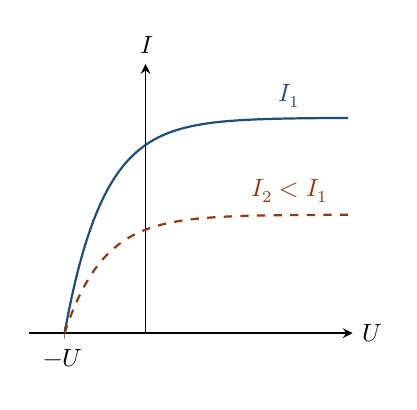
\begin{tikzpicture}
\begin{axis}[width=0.47\linewidth, height=5.0cm, axis lines=middle,
  xlabel={$U$}, ylabel={$I$}, xmin=-2.6, xmax=4.6, ymin=0, ymax=1.25,
  xtick={-1.8}, xticklabels={$-U_{\text з}$}, ytick=\empty,
  xlabel style={at={(ticklabel* cs:1)}, anchor=west},
  ylabel style={at={(ticklabel* cs:1)}, anchor=south}, clip=false]
  \addplot[domain=-1.8:4.5, samples=80, thick, accent]
     {1.0*(1-exp(-1.15*(x+1.8)))};
  \addplot[domain=-1.8:4.5, samples=80, thick, keycol, dashed]
     {0.55*(1-exp(-1.15*(x+1.8)))};
  \node[font=\small, accent] at (axis cs:3.2,1.1) {$I_1$};
  \node[font=\small, keycol] at (axis cs:3.2,0.66) {$I_2<I_1$};
\end{axis}
\end{tikzpicture}\hfill
\begin{tikzpicture}
\begin{axis}[width=0.47\linewidth, height=5.0cm, axis lines=middle,
  xlabel={$\nu$}, ylabel={$U_{\text з}$}, xmin=0, xmax=10, ymin=-2.2, ymax=4.2,
  xtick={4}, xticklabels={$\nu_0$}, ytick=\empty,
  xlabel style={at={(ticklabel* cs:1)}, anchor=west},
  ylabel style={at={(ticklabel* cs:1)}, anchor=south}, clip=false]
  \addplot[domain=4:9.5, thick, accent] {0.65*(x-4)};
  \addplot[domain=0:4, thin, dashed, gray] {0.65*(x-4)};
  \node[font=\small, anchor=west] at (axis cs:6.3,1.1) {$\tg\varphi = h/e$};
  \node[font=\small, anchor=west] at (axis cs:0.2,-2.0) {$-A/e$};
\end{axis}
\end{tikzpicture}
\caption{Слева: вольт-амперные характеристики фотоэлемента при одной и той же частоте и
двух интенсивностях света. Ток насыщения пропорционален интенсивности, задерживающее
напряжение $U_{\text з}$ одинаково. Справа: зависимость $U_{\text з}$ от частоты — прямая с
наклоном $h/e$, отсекающая на оси частот красную границу $\nu_0$ (качественно).}
\label{fig:1:photo}
\end{figure}

\paragraph{Почему не работает волновая картина.} В классической теории энергия, поглощаемая
электроном, пропорциональна интенсивности волны и времени облучения; поэтому $T_{\max}$ должна
расти с интенсивностью, красной границы быть не должно, а при слабом свете электрон должен
долго «накапливать» энергию. Оценка: пусть свет с интенсивностью $I=10^{-6}$~Вт/см$^2$
поглощается площадкой атомного размера $\sigma\sim10^{-15}$~см$^2$. Поглощаемая мощность
$I\sigma\sim10^{-21}$~Вт $\approx 6\cdot10^{-3}$~эВ/с, и для набора энергии $\sim2$~эВ
потребовалось бы $\sim 3\cdot 10^{2}$~с — в противоречии с безынерционностью фотоэффекта.
(Оценка предполагает, что электрон поглощает энергию лишь с площадки атомного размера.)

\subsection{Уравнение Эйнштейна}

\begin{principle}{Уравнение Эйнштейна для фотоэффекта}
Фотон поглощается одним электроном целиком. Энергия фотона расходуется на работу выхода
и сообщение электрону кинетической энергии:
\begin{equation}\label{eq:1:einstein}
  \hbar\omega = A + T_{\max},\qquad T_{\max}=\frac{\mel v_{\max}^2}{2}=eU_{\text з}.
\end{equation}
\end{principle}

Уравнение~\eqref{eq:1:einstein} объясняет все законы фотоэффекта.
(1) Число фотоэлектронов в единицу времени пропорционально числу поглощённых фотонов, т.\,е.
интенсивности — отсюда первый закон. (2) $T_{\max}$ определяется энергией одного фотона, а не
их числом. (3) При $\hbar\omega<A$ ни один фотон не может освободить электрон; многократное
поглощение при обычных интенсивностях маловероятно — отсюда красная граница. (4) Акт
поглощения фотона мгновенный, накапливать энергию не требуется.

Знак «max»: электроны, находящиеся глубже уровня Ферми или теряющие энергию при выходе из
металла, вылетают с меньшей энергией; уравнение~\eqref{eq:1:einstein} описывает электроны
с верхнего заполненного уровня, вылетевшие без потерь. Р.~Милликен (1916) проверил линейную
зависимость $U_{\text з}(\nu)$ и по её наклону $h/e$ определил постоянную Планка с точностью около
0{,}5\,\%. Характерные работы выхода: Cs — около 2~эВ ($\lambda_0\approx 0{,}6$~мкм, видимый
свет), Zn — около 4{,}3~эВ, Pt — около 5{,}6~эВ (ультрафиолет).

\begin{remark}
На опыте измеряется разность потенциалов между электродами, к которой добавляется контактная
разность потенциалов катод--анод. Она сдвигает прямую $U_{\text з}(\nu)$, но не меняет её
наклона $h/e$. При очень больших интенсивностях (лазеры) возможен многофотонный фотоэффект:
$N\hbar\omega=A+T_{\max}$, и красная граница в обычном смысле исчезает.
\end{remark}

\paragraph{Роль связанности электрона.} Свободный электрон не может поглотить фотон
(вывод~\ref{der:1:free}): законы сохранения энергии и импульса несовместимы. В фотоэффекте
избыточный импульс передаётся кристаллической решётке (или ядру атома в атомном фотоэффекте),
масса которых велика, поэтому энергию она практически не уносит. Именно поэтому фотоэффект
на атомах наиболее вероятен для электронов внутренних, сильно связанных оболочек.

\subsection{Эффект Комптона}

\paragraph{Опыт.} А.~Комптон (1923) рассеивал рентгеновское излучение (линия K$_\alpha$ молибдена,
$\lambda=0{,}071$~нм) на графите и измерял спектр рассеянного излучения кристаллическим
спектрометром при разных углах рассеяния $\theta$ (рис.~\ref{fig:1:compton}). Наблюдалось:
\begin{itemize}
 \item в рассеянном излучении присутствуют две линии — несмещённая ($\lambda$) и смещённая
       ($\lambda'>\lambda$);
 \item сдвиг $\Delta\lambda=\lambda'-\lambda$ растёт с углом рассеяния и не зависит ни от
       длины волны падающего излучения, ни от вещества рассеивателя;
 \item с ростом атомного номера рассеивателя интенсивность смещённой линии падает, а
       несмещённой растёт.
\end{itemize}
Классическая теория (томсоновское рассеяние) предсказывает, что электрон колеблется в поле волны
с её частотой и излучает на той же частоте, т.\,е. $\lambda'=\lambda$. Смещённая линия
классически необъяснима.

\paragraph{Объяснение.} Энергия рентгеновского фотона ($\hbar\omega\approx17$~кэВ) много больше
энергии связи внешних электронов лёгких атомов (единицы--десятки эВ), поэтому такие электроны
можно считать свободными и покоящимися. Рассеяние — упругое столкновение двух частиц:
фотона с импульсом $\hbar\vect k$ и электрона. Фотон отдаёт часть энергии электрону отдачи,
его частота уменьшается. Из законов сохранения (вывод~\ref{der:1:compton}):
\begin{equation}\label{eq:1:compton}
  \Delta\lambda=\lambda'-\lambda=\lC\,(1-\cos\theta)=2\lC\sin^2\frac{\theta}{2},\qquad
  \lC=\frac{h}{\mel c}.
\end{equation}
Сдвиг меняется от 0 (рассеяние вперёд) до $2\lC\approx4{,}85$~пм (рассеяние назад).
Для видимого света ($\lambda\sim500$~нм) относительный сдвиг $\Delta\lambda/\lambda\sim10^{-5}$,
поэтому эффект заметен лишь в рентгеновском и гамма-диапазонах.

\paragraph{Несмещённая линия.} Фотон может рассеяться на сильно связанном (внутреннем)
электроне так, что импульс отдачи получает атом как целое. В формулу~\eqref{eq:1:compton}
тогда входит масса атома $M\gg\mel$, и сдвиг $h/Mc$ ничтожен. Чем тяжелее атом, тем больше
доля сильно связанных электронов и тем интенсивнее несмещённая линия.

\begin{figure}[htbp]
\centering
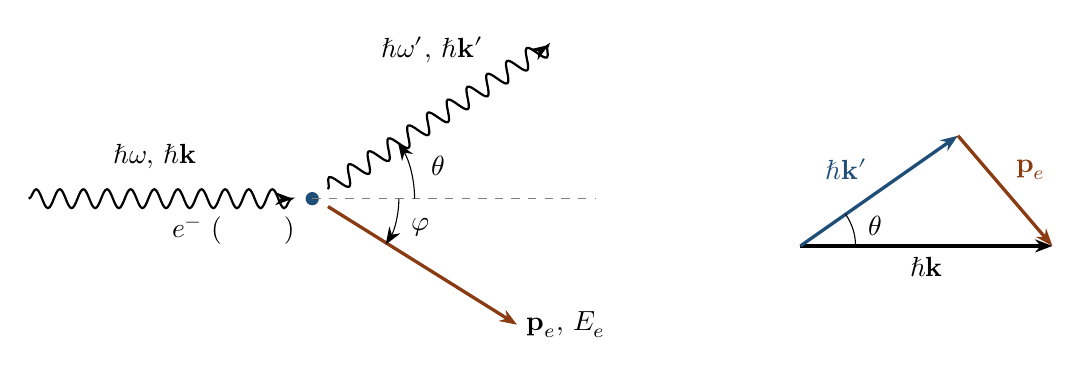
\begin{tikzpicture}[scale=1.0]
  \draw[thick, decorate, decoration={snake, amplitude=1.2mm, segment length=3mm}, ->]
     (-3.6,0) -- (-0.25,0);
  \node[above] at (-2.0,0.25) {$\hbar\omega,\ \hbar\vect k$};
  \fill[accent] (0,0) circle (2.4pt);
  \node[below left] at (-0.1,-0.1) {$e^-$ (покоится)};
  \draw[thick, decorate, decoration={snake, amplitude=1.2mm, segment length=3mm}, ->]
     (0.2,0.12) -- (3.0,1.95);
  \node[above left] at (2.3,1.6) {$\hbar\omega',\ \hbar\vect k'$};
  \draw[very thick, keycol, ->] (0.2,-0.1) -- (2.6,-1.6);
  \node[right] at (2.6,-1.6) {$\vect p_e,\ E_e$};
  \draw[dashed, gray] (0,0) -- (3.6,0);
  \draw[->] (1.3,0) arc[start angle=0, end angle=33, radius=1.3];
  \node at (1.6,0.42) {$\theta$};
  \draw[->] (1.1,0) arc[start angle=0, end angle=-32, radius=1.1];
  \node at (1.38,-0.36) {$\varphi$};
  % треугольник импульсов
  \begin{scope}[xshift=6.2cm, yshift=-0.6cm]
    \draw[very thick, ->] (0,0) -- (3.2,0) node[midway, below] {$\hbar\vect k$};
    \draw[very thick, accent, ->] (0,0) -- (2.0,1.4) node[midway, above left] {$\hbar\vect k'$};
    \draw[very thick, keycol, ->] (2.0,1.4) -- (3.2,0) node[midway, above right] {$\vect p_e$};
    \draw (0.7,0) arc[start angle=0, end angle=35, radius=0.7];
    \node at (0.95,0.25) {$\theta$};
  \end{scope}
\end{tikzpicture}
\caption{Геометрия эффекта Комптона (слева) и треугольник импульсов
$\hbar\vect k=\hbar\vect k'+\vect p_e$ (справа). $\theta$ — угол рассеяния фотона,
$\varphi$ — угол вылета электрона отдачи.}
\label{fig:1:compton}
\end{figure}

\section{Математические выводы}

\begin{derivation}[label=der:1:p]{импульс фотона}
Исходное соотношение — релятивистская связь энергии и импульса~\eqref{eq:1:Ep} и формула
для скорости $\vect v=\vect pc^2/E$. Требование $|\vect v|=c$ даёт $pc^2/E=c$, т.\,е.
$E=pc$. Подставив в~\eqref{eq:1:Ep}, получаем $m^2c^4=E^2-p^2c^2=0$. Тогда при $E=\hbar\omega$
\[
  p=\frac{E}{c}=\frac{\hbar\omega}{c}=\hbar k=\frac{h}{\lambda}.
\]
Размерность: $[\hbar k]=\text{эрг}\cdot\text{с}\cdot\text{см}^{-1}=\text{г}\cdot\text{см}/\text{с}$ —
размерность импульса.
\end{derivation}

\begin{derivation}[label=der:1:einst]{уравнение Эйнштейна и задерживающее напряжение}
\emph{Допущения:} фотон поглощается одним электроном; энергия связи наиболее слабо связанного
электрона металла равна работе выхода $A$; потерь при выходе нет.

Закон сохранения энергии для акта поглощения: $\hbar\omega = A + T_{\max}$.
Электрон, вылетевший с энергией $T_{\max}$, в тормозящем поле между катодом и анодом
теряет энергию $eU$. Ток прекращается, когда даже самые быстрые электроны не достигают анода:
\[
  T_{\max}=eU_{\text з}\quad\Longrightarrow\quad
  U_{\text з}=\frac{\hbar}{e}\,\omega-\frac{A}{e}=\frac{h}{e}\,(\nu-\nu_0),\qquad
  \nu_0=\frac{A}{h}.
\]
Наклон прямой $U_{\text з}(\nu)$ равен $h/e$ и не зависит от материала катода, а точка
пересечения с осью частот даёт красную границу. Длина волны красной границы
$\lambda_0=c/\nu_0=hc/A$; в удобных единицах $\lambda_0[\text{Å}]=12\,398/A[\text{эВ}]$.
\end{derivation}

\begin{derivation}[label=der:1:free]{свободный электрон не может поглотить фотон}
Перейдём в систему отсчёта, где электрон до поглощения покоится. До поглощения: энергия
$\hbar\omega+\mel c^2$, импульс $\hbar k$. После поглощения есть только электрон с энергией $E$ и
импульсом $p$. Законы сохранения:
\[
  \hbar\omega+\mel c^2=E,\qquad \hbar k=\frac{\hbar\omega}{c}=p .
\]
Подставим в релятивистское соотношение $E^2=p^2c^2+\mel^2c^4$:
\begin{align*}
  (\hbar\omega+\mel c^2)^2 &= (\hbar\omega)^2+\mel^2c^4,\\
  (\hbar\omega)^2+2\hbar\omega\,\mel c^2+\mel^2c^4 &= (\hbar\omega)^2+\mel^2c^4,\\
  2\hbar\omega\,\mel c^2 &=0 \quad\Longrightarrow\quad \omega=0 .
\end{align*}
Противоречие означает, что поглощение фотона свободным электроном невозможно.
Для фотоэффекта необходима «третья частица» (решётка, ядро), принимающая импульс.
\end{derivation}

\begin{derivation}[label=der:1:compton]{формула Комптона}
\emph{Допущения:} электрон свободен и до столкновения покоится; столкновение упругое;
используются релятивистские формулы (электрон отдачи может быть релятивистским).

\emph{Законы сохранения} энергии и импульса:
\begin{align}
  \hbar\omega+\mel c^2 &= \hbar\omega'+E_e, \label{eq:1:cE}\\
  \hbar\vect k &= \hbar\vect k'+\vect p_e. \label{eq:1:cp}
\end{align}
\emph{Шаг 1.} Из~\eqref{eq:1:cp} $\vect p_e=\hbar(\vect k-\vect k')$; возведём в квадрат,
учитывая, что угол между $\vect k$ и $\vect k'$ равен $\theta$ и $k=\omega/c$:
\[
  p_e^2c^2=\hbar^2\bigl(\omega^2+\omega'^2-2\omega\omega'\cos\theta\bigr).
\]
\emph{Шаг 2.} Из~\eqref{eq:1:cE} $E_e=\hbar(\omega-\omega')+\mel c^2$; возведём в квадрат:
\[
  E_e^2=\hbar^2(\omega-\omega')^2+2\hbar(\omega-\omega')\mel c^2+\mel^2c^4 .
\]
\emph{Шаг 3.} Подставим оба выражения в $E_e^2=p_e^2c^2+\mel^2c^4$:
\begin{align*}
  \hbar^2(\omega^2-2\omega\omega'+\omega'^2)+2\hbar(\omega-\omega')\mel c^2
     &=\hbar^2(\omega^2+\omega'^2-2\omega\omega'\cos\theta),\\
  2\hbar(\omega-\omega')\mel c^2 &= 2\hbar^2\omega\omega'(1-\cos\theta),\\
  \mel c^2\Bigl(\frac{1}{\omega'}-\frac{1}{\omega}\Bigr) &= \hbar(1-\cos\theta)
  \qquad\bigl(\text{деление на }2\hbar\,\omega\omega'\bigr).
\end{align*}
\emph{Шаг 4.} Переходя к длинам волн, $1/\omega=\lambda/(2\pi c)$:
\[
  \frac{\mel c^2}{2\pi c}(\lambda'-\lambda)=\hbar(1-\cos\theta)
  \quad\Longrightarrow\quad
  \boxed{\;\lambda'-\lambda=\frac{2\pi\hbar}{\mel c}(1-\cos\theta)=\lC(1-\cos\theta)\;}
\]
\emph{Проверка размерности:} $[h/(mc)]=\dfrac{\text{г}\cdot\text{см}^2/\text{с}}{\text{г}\cdot\text{см}/\text{с}}=\text{см}$.
\emph{Предельные случаи:} при $\theta=0$ сдвига нет (фотон не передаёт импульс); при
$\theta=\pi$ сдвиг максимален, $2\lC$.
\end{derivation}

\begin{derivation}[label=der:1:recoil]{энергии рассеянного фотона и электрона отдачи, угол отдачи}
Обозначим $\varepsilon=\hbar\omega/\mel c^2$. Из последней строки шага 3 вывода~\ref{der:1:compton}
$1/\omega'=1/\omega+\hbar(1-\cos\theta)/\mel c^2$, откуда
\begin{equation}\label{eq:1:omegap}
  \hbar\omega'=\frac{\hbar\omega}{1+\varepsilon(1-\cos\theta)} .
\end{equation}
Кинетическая энергия электрона отдачи $T_e=\hbar\omega-\hbar\omega'$:
\begin{equation}\label{eq:1:Te}
  T_e=\hbar\omega\,\frac{\varepsilon(1-\cos\theta)}{1+\varepsilon(1-\cos\theta)},\qquad
  T_e^{\max}=T_e(\theta=\pi)=\hbar\omega\,\frac{2\varepsilon}{1+2\varepsilon}.
\end{equation}
Угол вылета электрона $\varphi$ найдём из проекций~\eqref{eq:1:cp} на направление $\vect k$ и
перпендикулярное ему:
\[
  \hbar k=\hbar k'\cos\theta+p_e\cos\varphi,\qquad 0=\hbar k'\sin\theta-p_e\sin\varphi
  \;\Longrightarrow\;
  \tg\varphi=\frac{k'\sin\theta}{k-k'\cos\theta}.
\]
По~\eqref{eq:1:omegap} $k/k'=1+\varepsilon(1-\cos\theta)$, поэтому
\[
  \tg\varphi=\frac{\sin\theta}{1+\varepsilon(1-\cos\theta)-\cos\theta}
  =\frac{\sin\theta}{(1+\varepsilon)(1-\cos\theta)}
  =\frac{\ctg(\theta/2)}{1+\varepsilon},
\]
т.\,е. $\ctg\varphi=(1+\varepsilon)\tg(\theta/2)$.
Электрон отдачи всегда летит вперёд ($0\le\varphi\le\pi/2$).
\end{derivation}

\section{Итоговые формулы}

\keyformula{E=\hbar\omega,\qquad \vect p=\hbar\vect k,\qquad E=pc}
 {$\omega$ — круговая частота, $\vect k$ — волновой вектор ($k=2\pi/\lambda$), $\hbar=h/2\pi$.}
 {всегда для фотона в вакууме ($m=0$).}
 {связывает волновые характеристики излучения с корпускулярными.}

\keyformula{\hbar\omega=A+\frac{\mel v_{\max}^2}{2},\qquad eU_{\text з}=\hbar\omega-A,\qquad \omega_0=\frac{A}{\hbar}}
 {$A$ — работа выхода, $v_{\max}$ — максимальная скорость фотоэлектронов, $U_{\text з}$ — задерживающее напряжение.}
 {однофотонный фотоэффект, нерелятивистские фотоэлектроны.}
 {найти $T_{\max}$, красную границу, постоянную $h/e$ по наклону $U_{\text з}(\nu)$.}

\keyformula{\Delta\lambda=\lC(1-\cos\theta)=2\lC\sin^2\frac{\theta}{2},\qquad \lC=\frac{h}{\mel c}=2{,}43\pmet}
 {$\theta$ — угол рассеяния фотона, $\mel$ — масса электрона.}
 {рассеяние на свободном покоящемся электроне ($\hbar\omega\gg$ энергии связи).}
 {сдвиг длины волны; не зависит от $\lambda$ и вещества.}

\keyformula{\hbar\omega'=\frac{\hbar\omega}{1+\dfrac{\hbar\omega}{\mel c^2}(1-\cos\theta)},\qquad
  T_e^{\max}=\hbar\omega\frac{2\varepsilon}{1+2\varepsilon},\ \ \varepsilon=\frac{\hbar\omega}{\mel c^2}}
 {$\hbar\omega,\hbar\omega'$ — энергии падающего и рассеянного фотонов; $T_e$ — кинетическая энергия электрона отдачи.}
 {те же, что для формулы Комптона.}
 {энергия рассеянного кванта и максимальная энергия электрона отдачи («комптоновский край»).}

\section{Физическая интерпретация}

\textbf{Предельные случаи.} При $\hbar\omega\ll\mel c^2$ ($\varepsilon\ll1$) энергия фотона
почти не меняется, $\hbar\omega'\approx\hbar\omega$, — рассеяние переходит в классическое
томсоновское. При $\varepsilon\gg1$ фотон, рассеянный назад, имеет энергию $\hbar\omega'\to
\mel c^2/2\approx 0{,}26$~МэВ независимо от исходной: почти вся энергия уходит электрону.

\textbf{Смысл комптоновской длины волны.} $\lC$ — длина волны фотона с энергией $\mel c^2$
($\hbar\omega=\mel c^2\iff\lambda=h/\mel c$). Она задаёт масштаб, на котором проявляются
релятивистские квантовые эффекты: попытка локализовать электрон в области размером
$\Delta x\lesssim\hbar/\mel c$ требует импульсов $\Delta p\gtrsim\mel c$ и энергий $\gtrsim\mel c^2$,
достаточных для рождения электрон-позитронных пар. Иерархия атомных масштабов:
$r_e=\alpha\bar\lambda_{\mathrm C}$ (классический радиус), $\bar\lambda_{\mathrm C}$,
$\aB=\bar\lambda_{\mathrm C}/\alpha$, где $\alpha\approx1/137$.

\textbf{Связь с экспериментом.} Независимость $\Delta\lambda$ от вещества указывает, что
рассеяние идёт на электронах — частицах, одинаковых во всех веществах. Совпадение измеренного
$\Delta\lambda(\theta)$ с~\eqref{eq:1:compton} и регистрация электрона отдачи в совпадении с
рассеянным фотоном (опыты Боте и Гейгера, Комптона и Саймона) подтвердили, что энергия и
импульс сохраняются в каждом элементарном акте, а не только в среднем.

\textbf{Двойственность.} Ни волновая, ни корпускулярная модель по отдельности не описывает свет
полностью: в распространении и интерференции проявляются волновые свойства, а в обмене
энергией и импульсом с веществом — корпускулярные.

\section{Что необходимо знать на экзамене}

\begin{examcheck}
\checkhead{Определения}
\begin{itemize}
 \item фотон: $E=\hbar\omega$, $\vect p=\hbar\vect k$, $m=0$, два состояния поляризации;
 \item работа выхода, красная граница, задерживающее напряжение, ток насыщения;
 \item эффект Комптона; комптоновская длина волны $\lC=h/\mel c\approx2{,}43$~пм.
\end{itemize}
\checkhead{Формулы}
\begin{itemize}
 \item $\hbar\omega=A+T_{\max}$, $eU_{\text з}=\hbar\omega-A$, $\lambda_0=hc/A$;
 \item $\Delta\lambda=\lC(1-\cos\theta)$; $\hbar\omega'=\hbar\omega/[1+\varepsilon(1-\cos\theta)]$.
\end{itemize}
\checkhead{Выводы, которые нужно уметь воспроизвести}
\begin{itemize}
 \item $E=pc$ для частицы с $m=0$;
 \item невозможность поглощения фотона свободным электроном;
 \item формула Комптона из законов сохранения (шаги 1--4 вывода~\ref{der:1:compton}).
\end{itemize}
\checkhead{Интерпретации}
\begin{itemize}
 \item почему волновая теория не объясняет фотоэффект (интенсивность, красная граница, безынерционность);
 \item происхождение несмещённой линии; почему эффект не виден для видимого света;
 \item физический смысл $\lC$ как масштаба релятивистской локализации.
\end{itemize}
\end{examcheck}

% ======================================================================
\chapter[Волны де Бройля. Дифракция электронов. Соотношения неопределённостей]%
        {Волны де Бройля. Дифракция электронов. Соотношения неопределённостей}
\label{t:02}
% ======================================================================

\begin{qbox}
\textbf{Билет 2.} Волновые свойства массивных частиц — корпускулярно-волновой дуализм.
Опыты Девиссона--Джермера и Томсона по дифракции электронов. Длина волны де Бройля
нерелятивистской частицы. Соотношения неопределенностей (координата-импульс; энергия-время).
\end{qbox}

\section{Содержание билета}

\textbf{Подтемы:}
\begin{enumerate}
 \item гипотеза де Бройля и корпускулярно-волновой дуализм;
 \item длина волны де Бройля нерелятивистской частицы; электрон, ускоренный напряжением $U$;
 \item опыт Девиссона--Джермера (отражение от монокристалла) и опыт Томсона (прохождение через поликристаллическую фольгу);
 \item соотношение неопределённостей координата--импульс: формулировка, обоснование, примеры;
 \item соотношение неопределённостей энергия--время и его смысл.
\end{enumerate}

\textbf{Необходимые понятия:} фотон (\tref{t:01}); интерференция и дифракция волн;
условие Брэгга--Вульфа $2d\sin\vartheta=n\lambda$; фурье-разложение волнового пакета;
дисперсия (среднеквадратичное отклонение) случайной величины.

\section{Определения и физические принципы}

\begin{principle}{Гипотеза де Бройля (1924)}
С движением любой частицы с энергией $E$ и импульсом $\vect p$ связан волновой процесс
с частотой и волновым вектором
\begin{equation}\label{eq:2:dB}
 \omega=\frac{E}{\hbar},\qquad \vect k=\frac{\vect p}{\hbar},\qquad
 \lambda=\frac{2\pi}{k}=\frac{h}{p}.
\end{equation}
\end{principle}

\emph{Физический смысл.} Соотношения~\eqref{eq:2:dB} совпадают с соотношениями для фотона, но
применяются к частицам с ненулевой массой. Волна де Бройля — не классическая волна какого-либо
поля: её интенсивность определяет вероятность обнаружить частицу (статистическая трактовка
Борна, \tref{t:04}).

\begin{definition}[корпускулярно-волновой дуализм]
Свойство микрообъектов проявлять как корпускулярные (локализованная регистрация, сохранение
энергии и импульса в отдельном акте), так и волновые (интерференция, дифракция) свойства.
Какое из них проявляется, определяется условиями опыта; полное описание даёт квантовая механика.
\end{definition}

\begin{definition}[неопределённость]
Неопределённость величины $A$ в данном состоянии — среднеквадратичное отклонение результатов
её измерения от среднего по множеству одинаково приготовленных систем:
$\Delta A=\sqrt{\avg{(A-\avg A)^2}}$.
\end{definition}

\emph{Область применимости.} Волновые свойства существенны, когда длина волны де Бройля сравнима
с характерными размерами задачи (межатомные расстояния, размер атома, ширина щели). Для
макроскопических тел $\lambda$ ничтожно мала: пылинка массой $10^{-12}$~г со скоростью 1~см/с
имеет $\lambda=h/mv\approx7\cdot10^{-15}$~см, и волновые эффекты ненаблюдаемы.

\section{Основная теория}

\subsection{От фотона к частицам}

После опытов с фотоэффектом и эффектом Комптона стало ясно, что свет, считавшийся волной,
обладает корпускулярными свойствами. Л.~де Бройль предположил обратное: частицы вещества
обладают волновыми свойствами, причём связь между волновыми и корпускулярными характеристиками
та же, что у фотона. Аргумент: условие квантования Бора (\tref{t:03}) $L=n\hbar$ для круговой
орбиты эквивалентно требованию, чтобы на длине орбиты укладывалось целое число длин волн:
$2\pi r=n\lambda$, $\lambda=h/p$ $\Rightarrow$ $pr=n\hbar$.

\subsection{Длина волны де Бройля}

Для нерелятивистской частицы $p=mv=\sqrt{2mT}$, где $T$ — кинетическая энергия:
\begin{equation}\label{eq:2:lam}
  \lambda=\frac{h}{mv}=\frac{h}{\sqrt{2mT}}.
\end{equation}
Электрон, прошедший ускоряющую разность потенциалов $U$, имеет $T=eU$ и
\begin{equation}\label{eq:2:lamU}
  \lambda=\frac{h}{\sqrt{2\mel eU}}\approx\frac{12{,}26}{\sqrt{U[\text{В}]}}\ \text{Å}.
\end{equation}
При $U=100$~В $\lambda\approx1{,}23$~Å — порядок межатомных расстояний в кристаллах.
Поэтому кристалл служит дифракционной решёткой для электронов, как и для рентгеновских лучей.
Для частиц тепловых энергий $T\sim k_{\mathrm B}T_0$ ($T_0$ — температура) $\lambda\sim h/\sqrt{2mk_{\mathrm B}T_0}$:
для тепловых нейтронов при 300~К это $\approx 1{,}8$~Å, что используется в нейтронографии.

\begin{remark}[Релятивистская поправка]
При $eU\gtrsim0{,}01\,\mel c^2\approx5$~кэВ следует пользоваться точным выражением
$pc=\sqrt{T(T+2\mel c^2)}$, откуда
$\lambda=h\big/\sqrt{2\mel eU\,(1+eU/2\mel c^2)}$. Поправка $\approx eU/4\mel c^2$ к длине волны
важна в электронной микроскопии (100~кэВ — около 5\,\%).
\end{remark}

\subsection{Опыт Девиссона--Джермера (1927)}

Пучок электронов с энергией в десятки--сотни эВ падал нормально на грань монокристалла никеля;
детектор (цилиндр Фарадея) измерял ток отражённых электронов в зависимости от угла
(рис.~\ref{fig:2:dg}). При $U=54$~В под углом $\varphi=50^\circ$ к падающему пучку наблюдался
резкий максимум, который невозможно объяснить рассеянием частиц: он возникает только при
определённом напряжении.

\emph{Объяснение.} Поверхностный слой атомов — двумерная решётка с периодом $d=2{,}15$~Å
(расстояние между атомными рядами). Волны, рассеянные соседними рядами, усиливаются при
\begin{equation}\label{eq:2:grating}
  d\sin\varphi=n\lambda .
\end{equation}
При $n=1$: $\lambda=2{,}15\cdot\sin50^\circ\approx1{,}65$~Å. По формуле~\eqref{eq:2:lamU}
$\lambda=12{,}26/\sqrt{54}\approx1{,}67$~Å. Совпадение подтвердило формулу де Бройля
количественно. (Учёт преломления электронной волны на границе кристалла, где кинетическая энергия
электрона больше на величину внутреннего потенциала, устраняет оставшиеся небольшие расхождения
в положении максимумов высших порядков.)

\begin{figure}[htbp]
\centering
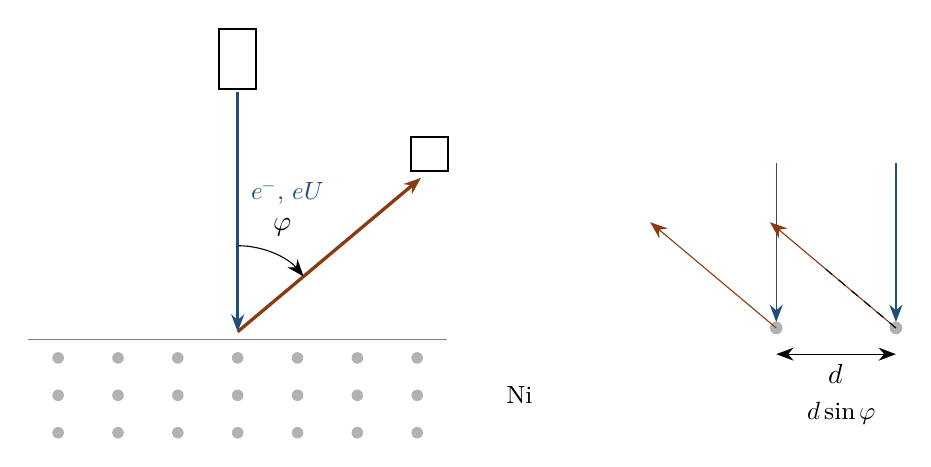
\begin{tikzpicture}[scale=0.95]
  % кристалл
  \foreach \x in {-2.4,-1.6,...,2.4} { \foreach \y in {0,-0.5,-1.0} { \fill[gray!60] (\x,\y) circle (2.2pt); } }
  \draw[gray] (-2.8,0.25) -- (2.8,0.25);
  \node[right, font=\small] at (2.6,-0.5) {кристалл Ni};
  % пушка
  \draw[thick] (-0.25,3.6) rectangle (0.25,4.4);
  \node[left, font=\small] at (-0.3,4.0) {электронная пушка};
  \draw[very thick, accent, ->] (0,3.55) -- (0,0.35);
  \node[right, font=\small, accent] at (0.05,2.2) {$e^-$, $eU$};
  % отражённый пучок
  \draw[very thick, keycol, ->] (0,0.35) -- ({0+3.2*sin(50)},{0.35+3.2*cos(50)});
  \draw[thick] ({3.35*sin(50)-0.25},{0.35+3.35*cos(50)}) rectangle ++(0.5,0.45);
  \node[right, font=\small] at ({3.35*sin(50)+0.3},{0.55+3.35*cos(50)}) {детектор};
  \draw[->] (0,1.5) arc[start angle=90, end angle=40, radius=1.15];
  \node at (0.6,1.75) {$\varphi$};
  % схема двух рядов
  \begin{scope}[xshift=7.2cm, yshift=0.4cm]
    \fill[gray!60] (0,0) circle (2.4pt); \fill[gray!60] (1.6,0) circle (2.4pt);
    \draw[<->] (0,-0.35) -- (1.6,-0.35) node[midway, below] {$d$};
    \draw[accent, ->] (0,2.2) -- (0,0.08); \draw[accent, ->] (1.6,2.2) -- (1.6,0.08);
    \draw[keycol, ->] (0,0) -- ({-2.2*sin(50)},{2.2*cos(50)});
    \draw[keycol, ->] (1.6,0) -- ({1.6-2.2*sin(50)},{2.2*cos(50)});
    \draw[dashed] (1.6,0) -- ({1.6*cos(50)*cos(50)},{1.6*cos(50)*sin(50)});
    \node[font=\small, align=left] at (0.2,-1.15) {разность хода $d\sin\varphi$};
  \end{scope}
\end{tikzpicture}
\caption{Опыт Девиссона--Джермера: схема установки (слева) и разность хода волн,
рассеянных соседними атомными рядами поверхности (справа).}
\label{fig:2:dg}
\end{figure}

\subsection{Опыт Томсона (1927)}

Дж.\,П.~Томсон пропускал пучок быстрых электронов (энергии $\sim$ 10--60~кэВ) через тонкую
($\sim10^{-6}$~см) поликристаллическую металлическую фольгу и регистрировал прошедшие электроны
на фотопластинке на расстоянии $L$ за фольгой. Наблюдалась система концентрических колец —
дебаеграмма, такая же, как при рентгеновской дифракции на поликристалле (метод Дебая--Шеррера).
Среди множества хаотически ориентированных микрокристаллов всегда есть такие, для которых
выполнено условие Брэгга--Вульфа
\begin{equation}\label{eq:2:bragg}
 2d\sin\vartheta=n\lambda ,
\end{equation}
где $d$ — межплоскостное расстояние, $\vartheta$ — угол скольжения. Отражённые лучи отклоняются
на угол $2\vartheta$ и образуют конус, т.\,е. кольцо радиуса $r\approx L\tg2\vartheta\approx2L\vartheta$.
При малых углах $\lambda\approx 2d\vartheta/n=d\,r/(nL)$, т.\,е. $r\propto\lambda\propto1/\sqrt U$, что
и наблюдалось. То, что кольца образованы именно электронами, а не вторичным рентгеновским
излучением, проверялось отклонением картины магнитным полем: кольца смещались целиком.

\paragraph{Дифракция одиночных частиц.} В опытах Л.~Бибермана, Н.~Сушкина и В.~Фабриканта (1949)
интенсивность пучка была столь мала, что электроны проходили прибор поодиночке. При длительной
экспозиции получалась та же дифракционная картина. Следовательно, волновые свойства присущи
каждому отдельному электрону, а не возникают от взаимодействия многих частиц. Аналогичные
результаты получены для нейтронов, атомов и молекул (вплоть до фуллеренов C$_{60}$).

\subsection{Соотношение неопределённостей координата--импульс}

\begin{principle}{Соотношение неопределённостей Гейзенберга}
В любом состоянии частицы неопределённости координаты и соответствующей проекции импульса
удовлетворяют неравенству
\begin{equation}\label{eq:2:HUP}
  \Delta x\,\Delta p_x\ge\frac{\hbar}{2},\qquad
  \Delta y\,\Delta p_y\ge\frac{\hbar}{2},\qquad
  \Delta z\,\Delta p_z\ge\frac{\hbar}{2}.
\end{equation}
Для «разноимённых» пар ($x$ и $p_y$) ограничений нет.
\end{principle}

\emph{Происхождение.} Частица с точно определённым импульсом описывается монохроматической
волной $\ee^{\ii p x/\hbar}$, распределённой по всему пространству, — её координата полностью
неопределённа. Чтобы локализовать частицу в области $\Delta x$, нужно сложить волны с разными
$k$ (волновой пакет). Из теории фурье-разложения известно, что ширины пакета в координатном и
$k$-пространствах связаны: $\Delta x\,\Delta k\gtrsim1$ (точнее, $\ge1/2$ для среднеквадратичных
ширин). С учётом $p=\hbar k$ это и есть~\eqref{eq:2:HUP}. Строгое доказательство для любых
операторов дано в \tref{t:05}; знак равенства достигается на гауссовом пакете
(вывод~\ref{der:2:gauss}).

\emph{Что соотношение НЕ означает.} Оно не связано с несовершенством приборов: это свойство
самого состояния. Частица не имеет одновременно определённых $x$ и $p_x$, поэтому понятие
траектории для микрочастиц теряет смысл. Классическое описание применимо, когда $\Delta x$ и
$\Delta p$, допускаемые~\eqref{eq:2:HUP}, пренебрежимо малы по сравнению с масштабами задачи.

\paragraph{Мысленный эксперимент: дифракция на щели.} Пусть частица с импульсом $p$ проходит
щель ширины $b$. Сразу после щели координата известна с точностью $\Delta x\sim b$. Из-за дифракции
частица отклоняется в пределах центрального максимума: $\sin\theta_1=\lambda/b$, т.\,е. приобретает
поперечный импульс $\Delta p_x\sim p\sin\theta_1=p\lambda/b=h/b$. Отсюда $\Delta x\,\Delta p_x\sim h$:
чем уже щель, тем шире дифракционная картина.

\subsection{Соотношение неопределённостей энергия--время}

\begin{principle}{Соотношение энергия--время}
\begin{equation}\label{eq:2:Et}
 \Delta E\,\Delta t\gtrsim\hbar .
\end{equation}
\end{principle}

Это соотношение имеет иной смысл, чем~\eqref{eq:2:HUP}: время в квантовой механике — параметр,
а не наблюдаемая с оператором. Существуют следующие корректные трактовки.
\begin{enumerate}
 \item \textbf{Время жизни и ширина уровня.} Состояние, существующее время $\tau$ (например,
       возбуждённое состояние атома), не имеет точно определённой энергии: его энергия размыта
       на ширину $\Gamma\approx\hbar/\tau$. Это проявляется как естественная ширина спектральной
       линии.
 \item \textbf{Длительность измерения.} Чтобы измерить энергию с точностью $\Delta E$, требуется
       время $\Delta t\gtrsim\hbar/\Delta E$ (волновой цуг длительности $\Delta t$ имеет ширину спектра
       $\Delta\omega\sim1/\Delta t$).
 \item \textbf{Характерное время изменения состояния.} Если $\Delta t$ — время, за которое средние
       значения величин заметно меняются, то разброс энергии в состоянии $\Delta E\gtrsim\hbar/\Delta t$
       (соотношение Мандельштама--Тамма, вывод опущен). Стационарное состояние ($\Delta E=0$) не
       меняется со временем вовсе.
\end{enumerate}

\section{Математические выводы}

\begin{derivation}[label=der:2:lamU]{длина волны электрона, ускоренного напряжением $U$}
Электрон, ускоренный из состояния покоя, приобретает кинетическую энергию $T=eU$. При
$eU\ll\mel c^2$ импульс $p=\sqrt{2\mel T}=\sqrt{2\mel eU}$, и
\[
 \lambda=\frac{h}{\sqrt{2\mel eU}}.
\]
Численно, используя $hc=12\,398$~эВ$\cdot$Å и $\mel c^2=0{,}511\cdot10^6$~эВ:
\[
 \lambda=\frac{hc}{\sqrt{2\,\mel c^2\,eU}}
 =\frac{12\,398\ \text{эВ}\cdot\text{Å}}{\sqrt{2\cdot0{,}511\cdot10^6\ \text{эВ}\cdot U[\text{В}]\ \text{эВ}}}
 =\frac{12\,398}{1011\sqrt{U[\text{В}]}}\ \text{Å}\approx\frac{12{,}26}{\sqrt{U[\text{В}]}}\ \text{Å}.
\]
Размерность: $[h/\sqrt{mT}]=\dfrac{\text{эрг}\cdot\text{с}}{\sqrt{\text{г}\cdot\text{эрг}}}=\dfrac{\text{г}\,\text{см}^2/\text{с}}{\text{г}\,\text{см}/\text{с}}=\text{см}$.
\end{derivation}

\begin{derivation}[label=der:2:packet]{оценка $\Delta x\,\Delta k\gtrsim 1$ для волнового пакета}
Рассмотрим пакет, составленный из волн с волновыми числами в интервале
$k_0-\Delta k/2<k<k_0+\Delta k/2$ с одинаковой амплитудой (момент $t=0$):
\[
 \psi(x)=\int_{k_0-\Delta k/2}^{k_0+\Delta k/2}\ee^{\ii kx}\,\dd k
 =\ee^{\ii k_0x}\,\frac{\ee^{\ii\Delta k\,x/2}-\ee^{-\ii\Delta k\,x/2}}{\ii x}
 =\ee^{\ii k_0x}\,\Delta k\,\frac{\sin(\Delta k\,x/2)}{\Delta k\,x/2}.
\]
Модуль огибающей максимален при $x=0$ и первый раз обращается в нуль при $\Delta k\,x/2=\pi$,
т.\,е. при $x=2\pi/\Delta k$. Принимая за ширину пакета половину расстояния между нулями,
$\Delta x\approx2\pi/\Delta k$, получаем $\Delta x\,\Delta k\approx2\pi$, а с $p=\hbar k$ —
$\Delta x\,\Delta p_x\approx h$. Конкретное число зависит от определения ширины, но
произведение не может быть сделано сколь угодно малым: сужение пакета в одном пространстве
неизбежно уширяет его в другом.
\end{derivation}

\begin{derivation}[label=der:2:gauss]{гауссов пакет: $\Delta x\,\Delta p_x=\hbar/2$}
Пусть $\psi(x)=(2\pi\sigma^2)^{-1/4}\exp\!\left(-\dfrac{x^2}{4\sigma^2}+\ii k_0x\right)$. Тогда
$|\psi|^2=(2\pi\sigma^2)^{-1/2}\ee^{-x^2/2\sigma^2}$ — нормальное распределение с дисперсией
$\sigma^2$, т.\,е. $\avg{x}=0$, $\Delta x=\sigma$.

Амплитуда распределения по $k$ — фурье-образ:
\[
 a(k)=\frac{1}{\sqrt{2\pi}}\int_{-\infty}^{\infty}\psi(x)\ee^{-\ii kx}\dd x
 =\frac{(2\pi\sigma^2)^{-1/4}}{\sqrt{2\pi}}\int_{-\infty}^{\infty}
   \exp\!\Bigl[-\frac{x^2}{4\sigma^2}-\ii(k-k_0)x\Bigr]\dd x .
\]
Используем интеграл Пуассона $\int_{-\infty}^{\infty}\ee^{-\alpha x^2-\ii\beta x}\dd x=\sqrt{\pi/\alpha}\,\ee^{-\beta^2/4\alpha}$
при $\alpha=1/4\sigma^2$, $\beta=k-k_0$:
\[
 a(k)\propto\exp\bigl[-\sigma^2(k-k_0)^2\bigr],\qquad
 |a(k)|^2\propto\exp\Bigl[-\frac{(k-k_0)^2}{2\,(1/2\sigma)^2}\Bigr].
\]
Это нормальное распределение с дисперсией $(1/2\sigma)^2$: $\Delta k=1/(2\sigma)$. Следовательно,
\[
 \Delta x\,\Delta k=\sigma\cdot\frac{1}{2\sigma}=\frac12,\qquad
 \Delta x\,\Delta p_x=\frac{\hbar}{2}.
\]
Гауссов пакет — состояние с минимально возможным произведением неопределённостей.
\end{derivation}

\begin{derivation}[label=der:2:atom]{оценка размера и энергии атома водорода из соотношения неопределённостей}
Электрон локализован в области размером $r$, поэтому $p\sim\Delta p\sim\hbar/r$. Энергия
\[
 E(r)\approx\frac{p^2}{2\mel}-\frac{e^2}{r}\approx\frac{\hbar^2}{2\mel r^2}-\frac{e^2}{r}.
\]
Минимизируем: $\dfrac{\dd E}{\dd r}=-\dfrac{\hbar^2}{\mel r^3}+\dfrac{e^2}{r^2}=0$
$\Rightarrow$ $r_0=\dfrac{\hbar^2}{\mel e^2}=\aB$, и
$E(r_0)=\dfrac{\hbar^2}{2\mel}\dfrac{\mel^2e^4}{\hbar^4}-\dfrac{\mel e^4}{\hbar^2}=-\dfrac{\mel e^4}{2\hbar^2}=-13{,}6\eV$.
Совпадение с точным результатом (\tref{t:10}) отчасти случайно (оценка верна по порядку
величины), но рассуждение показывает главное: \emph{атом устойчив потому, что сжатие электронного
облака увеличивает кинетическую энергию быстрее, чем уменьшает потенциальную.}
\end{derivation}

\begin{derivation}[label=der:2:nucleus]{почему электрон не может находиться в ядре}
Если бы электрон был локализован в области ядра $\Delta x\sim R\sim5\cdot10^{-13}$~см, то
$p\gtrsim\hbar/R$, и $pc\gtrsim\hbar c/R=197\MeV\cdot\text{фм}/5\fm\approx40$~МэВ $\gg\mel c^2$.
Электрон был бы ультрарелятивистским с энергией $\sim40$~МэВ, тогда как энергии электронов
бета-распада — порядка 1~МэВ, а глубина ядерного потенциала не удерживает электрон (на него
не действуют ядерные силы). Значит, электроны бета-распада рождаются в момент распада
(\tref{t:20}).
\end{derivation}

\section{Итоговые формулы}

\keyformula{\lambda=\frac{h}{p}=\frac{h}{mv},\qquad \vect k=\frac{\vect p}{\hbar},\qquad \omega=\frac{E}{\hbar}}
 {$p$ — импульс частицы, $m$ — масса, $v$ — скорость.}
 {любая частица; $p=mv$ — нерелятивистский случай.}
 {длина волны де Бройля; оценка роли волновых эффектов.}

\keyformula{\lambda=\frac{h}{\sqrt{2\mel eU}}\approx\frac{12{,}26}{\sqrt{U[\text{В}]}}\ \text{Å}}
 {$U$ — ускоряющее напряжение.}
 {электрон, $eU\ll\mel c^2$ (практически до нескольких кэВ).}
 {длина волны в опытах по дифракции электронов.}

\keyformula{d\sin\varphi=n\lambda\ \ \text{(Девиссон--Джермер)},\qquad 2d\sin\vartheta=n\lambda\ \ \text{(Брэгг--Вульф)}}
 {$d$ — период поверхностной решётки / межплоскостное расстояние, $\varphi$ — угол отражения от нормали, $\vartheta$ — угол скольжения, $n$ — порядок.}
 {однократное (кинематическое) рассеяние; без учёта преломления на поверхности.}
 {связь положения дифракционных максимумов с $\lambda$.}

\keyformula{\Delta x\,\Delta p_x\ge\frac{\hbar}{2},\qquad \Delta E\,\Delta t\gtrsim\hbar,\qquad \Gamma\tau\approx\hbar}
 {$\Delta$ — среднеквадратичные отклонения; $\Gamma$ — ширина уровня, $\tau$ — время жизни.}
 {первое — строгое неравенство для любого состояния; второе — оценочное, $t$ — не наблюдаемая.}
 {оценки размеров и энергий связанных состояний, ширины линий, времён жизни.}

\section{Физическая интерпретация}

\textbf{Масштабы.} $\lambda\propto1/\sqrt{mT}$: при одинаковой энергии тяжёлые частицы имеют
меньшую длину волны ($\lambda_p/\lambda_e=\sqrt{\mel/m_p}\approx1/43$). Электроны с энергией
100~эВ и рентгеновские фотоны с энергией $\sim10$~кэВ имеют длины волн порядка ангстрема —
отсюда электронография и рентгеноструктурный анализ. Высокая разрешающая способность электронного
микроскопа обусловлена малостью $\lambda$ при энергиях 100--300~кэВ.

\textbf{Классический предел.} Классическая механика применима, если $\lambda$ мала по сравнению
с масштабом изменения потенциала, а неопределённости, следующие из~\eqref{eq:2:HUP},
пренебрежимы: например, для электрона в кинескопе ($\Delta x\sim10^{-3}$~см) $\Delta v\sim\hbar/(\mel\Delta x)\sim10^3$~см/с
при $v\sim10^9$~см/с — траекторию можно использовать. Для электрона в атоме $\Delta v\sim v$ —
понятие орбиты теряет смысл.

\textbf{Энергия нулевых колебаний.} Частица, запертая в области размера $a$, не может иметь
нулевую кинетическую энергию: $E_{\min}\sim\hbar^2/(ma^2)$. Это объясняет конечную энергию
основного состояния в яме (\tref{t:06}) и осцилляторе (\tref{t:08}).

\textbf{Ширина линий.} Время жизни возбуждённого атома $\tau\sim10^{-8}$~с даёт $\Gamma\sim\hbar/\tau\sim
7\cdot10^{-8}$~эВ — естественная ширина линии. Короткоживущие адроны ($\tau\sim10^{-23}$~с) имеют
ширины $\sim100$~МэВ, и их «масса» определяется лишь с такой точностью (\tref{t:15}).

\section{Что необходимо знать на экзамене}

\begin{examcheck}
\checkhead{Определения}
\begin{itemize}
 \item гипотеза де Бройля: $\lambda=h/p$, $\omega=E/\hbar$; смысл корпускулярно-волнового дуализма;
 \item неопределённость как среднеквадратичное отклонение.
\end{itemize}
\checkhead{Формулы}
\begin{itemize}
 \item $\lambda=h/\sqrt{2mT}$, $\lambda\approx12{,}26/\sqrt{U}$~Å;
 \item $d\sin\varphi=n\lambda$, $2d\sin\vartheta=n\lambda$;
 \item $\Delta x\,\Delta p_x\ge\hbar/2$, $\Delta E\,\Delta t\gtrsim\hbar$.
\end{itemize}
\checkhead{Выводы и оценки}
\begin{itemize}
 \item численная обработка опыта Девиссона--Джермера: 54~В, $50^\circ$, $d=2{,}15$~Å $\Rightarrow$ $\lambda\approx1{,}65$~Å;
 \item оценка $\Delta x\,\Delta k\sim2\pi$ для пакета; дифракция на щели;
 \item оценка размера и энергии атома водорода; невозможность электрона в ядре.
\end{itemize}
\checkhead{Интерпретации}
\begin{itemize}
 \item чем различаются опыты Девиссона--Джермера и Томсона; как доказано, что кольца дают электроны;
 \item дифракция одиночных электронов — волновые свойства присущи каждой частице;
 \item смысл соотношения энергия--время (время жизни и ширина уровня).
\end{itemize}
\end{examcheck}

% ======================================================================
\chapter[Постулаты Бора. Атом водорода. Водородоподобные атомы]%
        {Постулаты Бора. Атом водорода и водородоподобные системы}
\label{t:03}
% ======================================================================

\begin{qbox}
\textbf{Билет 3.} Постулаты Бора для атома водорода. Характерные параметры для атома
водорода: боровский радиус, скорость электрона, уровни энергии. Водородоподобные атомы:
влияние массы ядра (изотопический сдвиг), атомы щелочных металлов, многозарядные ионы, мезоатомы.
\end{qbox}

\section{Содержание билета}

\textbf{Подтемы:}
\begin{enumerate}
 \item постулаты Бора; правило квантования момента импульса;
 \item радиусы орбит, скорости, энергии уровней; боровский радиус, постоянная тонкой структуры;
 \item спектральные серии водорода, формула Ридберга;
 \item учёт конечной массы ядра: приведённая масса, изотопический сдвиг (H и D);
 \item атомы щелочных металлов: квантовый дефект;
 \item многозарядные (водородоподобные) ионы: масштабирование по $Z$;
 \item мезоатомы (мюонные атомы), позитроний.
\end{enumerate}

\textbf{Необходимые понятия:} кулоновское взаимодействие, движение по окружности,
задача двух тел и центр масс, фотон $\hbar\omega$ (\tref{t:01}), волна де Бройля (\tref{t:02}).

\section{Определения и физические принципы}

\begin{principle}{Постулаты Бора (1913)}
\begin{enumerate}[leftmargin=1.4em]
 \item \emph{Постулат стационарных состояний.} Атом может длительно находиться только в
       определённых стационарных состояниях с дискретными энергиями $E_1<E_2<\dots$; находясь
       в них, атом не излучает, несмотря на ускоренное движение электрона.
 \item \emph{Правило частот.} При переходе атома из состояния $n$ в состояние $m$ испускается
       (или поглощается) фотон с частотой
       \begin{equation}\label{eq:3:freq}
          \hbar\omega_{nm}=E_n-E_m .
       \end{equation}
 \item \emph{Правило квантования} (для круговых орбит). В стационарных состояниях момент
       импульса электрона кратен $\hbar$:
       \begin{equation}\label{eq:3:quant}
          L=\mu vr=n\hbar,\qquad n=1,2,3,\dots
       \end{equation}
\end{enumerate}
\end{principle}

\emph{Физический смысл и проблема.} По классической электродинамике электрон, движущийся с
ускорением по орбите, должен излучать и за время $\sim10^{-11}$~с упасть на ядро; спектр
излучения должен быть сплошным. Опыт показывает устойчивость атомов и линейчатые спектры.
Постулаты Бора \emph{вводят} дискретность как новый принцип, не объясняя её. Правило
квантования~\eqref{eq:3:quant} эквивалентно условию, что на орбите укладывается целое число
волн де Бройля: $2\pi r=n\lambda=nh/(\mu v)$.

\begin{definition}[характерные атомные величины]
\begin{align*}
 &\text{боровский радиус}&& \aB=\frac{\hbar^2}{\mel e^2}=0{,}529\ \text{Å},\\
 &\text{постоянная тонкой структуры}&& \alpha=\frac{e^2}{\hbar c}\approx\frac{1}{137},\\
 &\text{энергия Ридберга}&& \Ry=\frac{\mel e^4}{2\hbar^2}=\frac{e^2}{2\aB}=\frac{\alpha^2\mel c^2}{2}=13{,}6\eV .
\end{align*}
\end{definition}

\begin{definition}[водородоподобная система]
Система из одного электрона (или другой отрицательно заряженной частицы) и ядра с зарядом $Ze$,
либо система, в которой один внешний электрон движется в поле, близком к кулоновскому
(атомы щелочных металлов).
\end{definition}

\emph{Область применимости модели Бора.} Модель даёт точные уровни энергии для кулоновской
задачи (совпадающие с решением уравнения Шредингера, \tref{t:10}), если движение
нерелятивистское ($Z\alpha\ll1$). Модель не объясняет интенсивности линий, не применима к
многоэлектронным атомам (уже к He), неверно предсказывает момент импульса основного
состояния ($\hbar$ вместо 0) и противоречит соотношению неопределённостей (точные орбиты).

\section{Основная теория}

\subsection{Уровни энергии атома водорода}

Решение системы «второй закон Ньютона + правило квантования» (вывод~\ref{der:3:bohr})
для частицы с зарядом $-e$ и приведённой массой $\mu$ в поле ядра с зарядом $Ze$:
\begin{equation}\label{eq:3:levels}
  r_n=\frac{\hbar^2}{\mu Ze^2}\,n^2,\qquad
  v_n=\frac{Ze^2}{n\hbar}=\frac{Z\alpha c}{n},\qquad
  E_n=-\frac{\mu Z^2e^4}{2\hbar^2}\frac{1}{n^2}.
\end{equation}
Для водорода ($Z=1$, $\mu\approx\mel$):
\begin{center}
\begin{tabular}{@{}ll@{}}
\toprule
радиус первой орбиты & $r_1=\aB=0{,}529$~Å \\
скорость на первой орбите & $v_1=\alpha c=2{,}19\cdot10^8$~см/с $\approx c/137$ \\
энергия основного состояния & $E_1=-\Ry=-13{,}6$~эВ (энергия ионизации 13{,}6~эВ) \\
период обращения & $T_1=2\pi\aB/v_1\approx1{,}5\cdot10^{-16}$~с \\
напряжённость поля ядра на орбите & $e/\aB^2\approx5\cdot10^9$~В/см \\
\bottomrule
\end{tabular}
\end{center}
Малость $v_1/c=\alpha$ оправдывает нерелятивистское описание; релятивистские поправки к уровням
имеют относительную величину $\sim\alpha^2\sim5\cdot10^{-5}$ (тонкая структура).

\subsection{Спектральные серии}

Из~\eqref{eq:3:freq} и~\eqref{eq:3:levels} (вывод~\ref{der:3:rydberg}):
\begin{equation}\label{eq:3:rydberg}
  \frac{1}{\lambda_{nm}}=R\,Z^2\left(\frac{1}{m^2}-\frac{1}{n^2}\right),\qquad n>m,
\end{equation}
где $R=\mu e^4/(4\pi\hbar^3c)$ — постоянная Ридберга. Линии с общим нижним уровнем $m$
образуют серию (рис.~\ref{fig:3:levels}): $m=1$ — серия Лаймана (УФ, 91--122~нм),
$m=2$ — серия Бальмера (видимая, $\mathrm H_\alpha=656{,}3$~нм, граница 364,6~нм),
$m=3$ — Пашена (ИК), $m=4$ — Брэккета, $m=5$ — Пфунда. При $n\to\infty$ линии сгущаются к
\emph{границе серии}, за которой лежит сплошной спектр (переходы с ионизацией).

\begin{figure}[htbp]
\centering
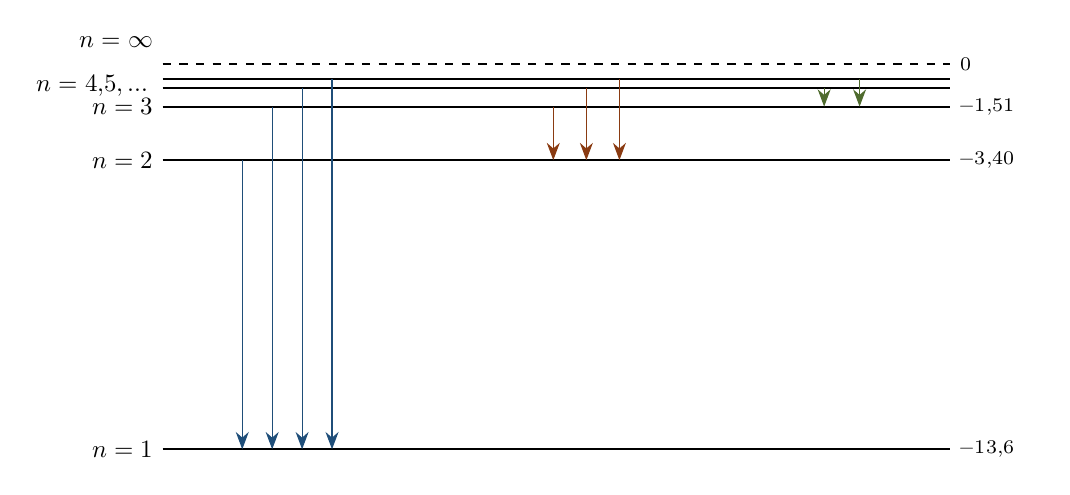
\begin{tikzpicture}[yscale=0.36, xscale=1.0]
  \foreach \n in {1,2,3,4,5} { \draw[thick] (0,{-13.6/(\n*\n)}) -- (10,{-13.6/(\n*\n)}); }
  \foreach \n/\val in {1/{-13,6},2/{-3,40},3/{-1,51}} {
     \node[left, font=\small] at (0,{-13.6/(\n*\n)}) {$n=\n$};
     \node[right, font=\scriptsize] at (10,{-13.6/(\n*\n)}) {$\val$ эВ};
  }
  \node[left, font=\small] at (0,-0.75) {$n=4,5,\dots$};
  \draw[thick, dashed] (0,0) -- (10,0) node[right, font=\scriptsize] {$0$};
  \node[left, font=\small] at (0,0.75) {$n=\infty$};
  \foreach \n in {2,3,4,5} { \draw[accent, ->] ({0.25+0.38*\n},{-13.6/(\n*\n)}) -- ({0.25+0.38*\n},-13.6); }
  \node[accent, font=\small, anchor=east] at (0.95,-8.0) {Лайман};
  \foreach \n in {3,4,5} { \draw[keycol, ->] ({3.7+0.42*\n},{-13.6/(\n*\n)}) -- ({3.7+0.42*\n},-3.4); }
  \node[keycol, font=\small] at (5.4,-4.6) {Бальмер};
  \foreach \n in {4,5} { \draw[dercol, ->] ({6.6+0.45*\n},{-13.6/(\n*\n)}) -- ({6.6+0.45*\n},{-13.6/9}); }
  \node[dercol, font=\small] at (8.6,-2.3) {Пашен};
\end{tikzpicture}
\caption{Уровни энергии атома водорода $E_n=-13{,}6/n^2$~эВ (в масштабе) и переходы,
образующие серии Лаймана, Бальмера и Пашена.}
\label{fig:3:levels}
\end{figure}

\subsection{Влияние массы ядра. Изотопический сдвиг}

Ядро имеет конечную массу $M$, поэтому электрон и ядро вращаются вокруг общего центра масс.
Задача двух тел сводится к движению одной частицы с \emph{приведённой массой}
\begin{equation}
  \mu=\frac{\mel M}{\mel+M}=\frac{\mel}{1+\mel/M}
\end{equation}
по относительной координате (вывод~\ref{der:3:reduced}). Все формулы~\eqref{eq:3:levels}
сохраняются с заменой $\mel\to\mu$; в частности,
\begin{equation}\label{eq:3:RM}
  R_M=\frac{R_\infty}{1+\mel/M},\qquad R_\infty=\frac{\mel e^4}{4\pi\hbar^3c}=109\,737\ \text{см}^{-1}.
\end{equation}
Для водорода $R_{\mathrm H}=109\,678$~см$^{-1}$. Изотопы одного элемента имеют разные $M$, и их
линии сдвинуты: \emph{изотопический сдвиг}. Для водорода и дейтерия ($M_D\approx2M_p$)
(вывод~\ref{der:3:isotope})
\begin{equation}\label{eq:3:shift}
  \frac{\lambda_{\mathrm H}-\lambda_{\mathrm D}}{\lambda_{\mathrm H}}
  \approx\frac{\mel}{M_p}-\frac{\mel}{M_D}\approx\frac{\mel}{2M_p}=2{,}7\cdot10^{-4}.
\end{equation}
Для линии $\mathrm H_\alpha$ ($656{,}3$~нм) сдвиг $\approx0{,}18$~нм — линия дейтерия смещена в
коротковолновую сторону. По такому слабому спутнику линий Бальмера Г.~Юри в 1932~г. открыл
дейтерий. (У тяжёлых атомов изотопический сдвиг определяется в основном не массой, а различием
размеров ядер — «объёмный эффект».)

\subsection{Атомы щелочных металлов}

В атомах Li, Na, K, Rb, Cs один валентный электрон находится вне заполненных оболочек
(«атомного остатка» с зарядом $+e$). Вдали от остатка электрон движется в кулоновском поле
заряда $+e$, но вблизи — в поле не полностью экранированного ядра. Отклонение от кулоновского
поля тем сильнее, чем глубже электрон проникает в остаток, т.\,е. чем меньше его орбитальный
момент $l$ (\tref{t:09}). Эмпирически уровни описываются формулой Ридберга
\begin{equation}\label{eq:3:qd}
  E_{nl}=-\frac{\Ry}{(n-\Delta_l)^2}=-\frac{\Ry}{n^{*2}},
\end{equation}
где $\Delta_l$ — \emph{квантовый дефект}, почти не зависящий от $n$, но зависящий от $l$; $n^*$ —
эффективное главное квантовое число. Для натрия $\Delta_s\approx1{,}37$, $\Delta_p\approx0{,}88$,
$\Delta_d\approx0{,}01$. Отсюда $E_{3s}\approx-13{,}6/(1{,}63)^2\approx-5{,}1$~эВ (потенциал ионизации
Na равен 5,14~эВ), а переход $3p\to3s$ даёт $\approx2{,}1$~эВ — жёлтая D-линия
($\lambda\approx589$~нм). Вырождение по $l$, характерное для чистого кулоновского поля, снимается.
Причины $\Delta_l\neq0$: проникновение электрона в остов и поляризация остова.

\subsection{Многозарядные ионы}

Ионы He$^+$, Li$^{2+}$, Be$^{3+}$,\,\dots, U$^{91+}$ имеют один электрон и ядро с зарядом $Ze$.
По~\eqref{eq:3:levels}
\begin{equation}
  r_n=\frac{\aB n^2}{Z},\qquad v_n=\frac{Z\alpha c}{n},\qquad E_n=-\frac{Z^2\Ry}{n^2}.
\end{equation}
Размеры уменьшаются в $Z$ раз, энергии растут в $Z^2$ раз. Для He$^+$ $E_1=-54{,}4$~эВ; серия
Пикеринга иона He$^+$ (переходы на $n=4$) содержит линии, почти совпадающие с линиями Бальмера,
так как $Z^2/n^2=4/(2k)^2=1/k^2$; небольшое различие обусловлено разными приведёнными массами.
С ростом $Z$ скорость $v_1=Z\alpha c$ становится сравнимой с $c$ (для U$^{91+}$ $v_1\approx0{,}67c$,
$|E_1|\approx115$~кэВ), и необходим релятивистский расчёт. Сходный закон $Z^2$ действует для
рентгеновских K-линий тяжёлых атомов: электрон, переходящий на вакансию в K-оболочке, «видит»
заряд $(Z-1)e$, что даёт закон Мозли $\hbar\omega_{K_\alpha}\approx\frac34\Ry\,(Z-1)^2$.

\subsection{Мезоатомы и экзотические атомы}

Отрицательный мюон ($m_\mu=206{,}8\,\mel$, время жизни 2,2~мкс), захваченный ядром, образует
\emph{мюонный атом}. Мюон каскадно переходит на нижние уровни за время $\sim10^{-13}$~с, много
меньшее времени жизни. В~\eqref{eq:3:levels} масса $\mel$ заменяется приведённой массой
$\mu=m_\mu M/(m_\mu+M)$:
\begin{itemize}
 \item мюонный водород ($\mu p$): $\mu=185{,}8\,\mel$, $r_1=\aB/185{,}8\approx285$~фм,
       $E_1=-185{,}8\cdot13{,}6\eV\approx-2{,}5$~кэВ;
 \item тяжёлые ядра: для свинца ($Z=82$) $r_1\approx\aB\mel/(207\cdot82)\approx3$~фм — меньше
       радиуса ядра ($\approx7$~фм). Мюон значительную часть времени проводит внутри ядра, и
       его уровни чувствительны к распределению заряда в ядре. Измерение рентгеновских линий
       мюонных атомов — один из методов определения размеров ядер (\tref{t:17}).
\end{itemize}
Существуют также пионные, каонные, антипротонные атомы. \emph{Позитроний} ($e^+e^-$) —
водородоподобная система с $\mu=\mel/2$: $E_1=-6{,}8$~эВ, расстояние между частицами в
основном состоянии вдвое больше $\aB$.

\section{Математические выводы}

\begin{derivation}[label=der:3:bohr]{радиусы, скорости и энергии стационарных орбит}
\emph{Допущения:} ядро с зарядом $Ze$; движение нерелятивистское, по окружности; масса
частицы $\mu$ (приведённая, см. вывод~\ref{der:3:reduced}).

\emph{Исходные уравнения:} второй закон Ньютона (кулоновская сила — центростремительная)
и правило квантования:
\begin{equation}\label{eq:3:sys}
  \frac{\mu v^2}{r}=\frac{Ze^2}{r^2},\qquad \mu vr=n\hbar .
\end{equation}
\emph{Шаг 1.} Умножим первое уравнение на $r^2$: $\mu v^2r=Ze^2$. Разделим на второе:
\[
  \frac{\mu v^2 r}{\mu vr}=\frac{Ze^2}{n\hbar}\quad\Longrightarrow\quad v_n=\frac{Ze^2}{n\hbar}
  =\frac{e^2}{\hbar c}\frac{Zc}{n}=\frac{Z\alpha c}{n}.
\]
\emph{Шаг 2.} Из правила квантования
\[
  r_n=\frac{n\hbar}{\mu v_n}=\frac{n\hbar\cdot n\hbar}{\mu Ze^2}=\frac{\hbar^2}{\mu Ze^2}n^2 .
\]
\emph{Шаг 3.} Полная энергия $E=T+U$, $T=\mu v^2/2$, $U=-Ze^2/r$. Из первого уравнения~\eqref{eq:3:sys}
$\mu v^2=Ze^2/r$, поэтому
\[
  T=\frac{Ze^2}{2r}=-\frac{U}{2},\qquad E=T+U=-\frac{Ze^2}{2r}=-T .
\]
(Это частный случай теоремы вириала для кулоновского поля: $2\bar T=-\bar U$.)
\emph{Шаг 4.} Подставим $r_n$:
\[
  E_n=-\frac{Ze^2}{2}\cdot\frac{\mu Ze^2}{\hbar^2n^2}=-\frac{\mu Z^2e^4}{2\hbar^2}\frac{1}{n^2}.
\]
\emph{Проверка размерности:} $[\mu e^4/\hbar^2]=\text{г}\cdot(\text{эрг}\cdot\text{см})^2/(\text{эрг}\cdot\text{с})^2=\text{г}\,\text{см}^2/\text{с}^2=\text{эрг}$;
$[\hbar^2/\mu e^2]=(\text{эрг}\,\text{с})^2/(\text{г}\cdot\text{эрг}\,\text{см})=\text{см}$.
\emph{Численно} ($Z=1$, $\mu=\mel$):
\[
 \aB=\frac{(\hbar c)^2}{\mel c^2\,e^2}=\frac{(1973{,}3\ \text{эВ}\cdot\text{Å})^2}{0{,}511\cdot10^6\ \text{эВ}\cdot14{,}40\ \text{эВ}\cdot\text{Å}}=0{,}529\ \text{Å},
\]
\[
 \Ry=\frac{e^2}{2\aB}=\frac{14{,}40}{2\cdot0{,}529}\ \text{эВ}=13{,}6\ \text{эВ}.
\]
\end{derivation}

\begin{derivation}[label=der:3:rydberg]{формула Ридберга}
По правилу частот~\eqref{eq:3:freq} и формуле~\eqref{eq:3:levels}:
\[
  \hbar\omega_{nm}=E_n-E_m=\frac{\mu Z^2e^4}{2\hbar^2}\Bigl(\frac{1}{m^2}-\frac{1}{n^2}\Bigr).
\]
С учётом $\omega=2\pi c/\lambda$:
\[
  \frac{1}{\lambda}=\frac{\omega}{2\pi c}=\frac{\mu e^4}{4\pi\hbar^3c}\,Z^2\Bigl(\frac{1}{m^2}-\frac{1}{n^2}\Bigr)
  \equiv R\,Z^2\Bigl(\frac{1}{m^2}-\frac{1}{n^2}\Bigr).
\]
Пример: $\mathrm H_\alpha$ ($3\to2$): $1/\lambda=R_{\mathrm H}(1/4-1/9)=R_{\mathrm H}\cdot5/36$,
$\lambda=36/(5\cdot109\,678\ \text{см}^{-1})=6{,}565\cdot10^{-5}$~см (в вакууме; в воздухе 656,3~нм).
\end{derivation}

\begin{derivation}[label=der:3:reduced]{приведённая масса}
Пусть $\vect r_e$, $\vect r_N$ — радиус-векторы электрона и ядра, потенциал зависит только от
$\vect r=\vect r_e-\vect r_N$. Введём центр масс $\vect R=(\mel\vect r_e+M\vect r_N)/(\mel+M)$.
Тогда $\vect r_e=\vect R+\frac{M}{\mel+M}\vect r$, $\vect r_N=\vect R-\frac{\mel}{\mel+M}\vect r$, и
кинетическая энергия
\[
  T=\frac{\mel\dot{\vect r}_e^{\,2}}{2}+\frac{M\dot{\vect r}_N^{\,2}}{2}
   =\frac{(\mel+M)\dot{\vect R}^2}{2}+\frac12\Bigl(\frac{\mel M^2}{(\mel+M)^2}+\frac{M\mel^2}{(\mel+M)^2}\Bigr)\dot{\vect r}^{\,2}
   =\frac{(\mel+M)\dot{\vect R}^2}{2}+\frac{\mu\dot{\vect r}^{\,2}}{2}
\]
(перекрёстные члены $\propto\dot{\vect R}\cdot\dot{\vect r}$ сокращаются). В системе центра масс
($\dot{\vect R}=0$) задача сводится к движению одной частицы массы $\mu=\mel M/(\mel+M)$ в поле
$U(r)$; полный момент импульса равен $\mu r v$, где $v=|\dot{\vect r}|$. Поэтому в~\eqref{eq:3:sys}
стоит $\mu$, а уровни $E_n\propto\mu$.
\end{derivation}

\begin{derivation}[label=der:3:isotope]{изотопический сдвиг H--D}
Для линии одного и того же перехода $\lambda\propto1/R_M\propto1+\mel/M$. Тогда
\begin{align*}
  \frac{\lambda_{\mathrm D}}{\lambda_{\mathrm H}}&=\frac{1+\mel/M_D}{1+\mel/M_p}
  \approx1-\frac{\mel}{M_p}+\frac{\mel}{M_D},\\
  \frac{\lambda_{\mathrm H}-\lambda_{\mathrm D}}{\lambda_{\mathrm H}}&\approx\frac{\mel}{M_p}-\frac{\mel}{M_D}
  \approx\frac{\mel}{M_p}\Bigl(1-\frac12\Bigr)=\frac{1}{2\cdot1836}=2{,}72\cdot10^{-4},
\end{align*}
где отброшены члены порядка $(\mel/M)^2$. Для $\mathrm H_\alpha$: $\Delta\lambda=656{,}3\cdot2{,}72\cdot10^{-4}\approx0{,}18$~нм.
\end{derivation}

\begin{derivation}[label=der:3:corr]{принцип соответствия для больших $n$}
Частота излучения при переходе $n\to n-1$ при $n\gg1$:
\[
  \omega_{n,n-1}=\frac{E_n-E_{n-1}}{\hbar}\approx\frac{1}{\hbar}\frac{\dd E_n}{\dd n}
  =\frac{1}{\hbar}\cdot\frac{\mu Z^2e^4}{\hbar^2n^3}=\frac{\mu Z^2e^4}{\hbar^3n^3}.
\]
Классическая частота обращения по $n$-й орбите:
$\omega_{\text{орб}}=\dfrac{v_n}{r_n}=\dfrac{Ze^2}{n\hbar}\cdot\dfrac{\mu Ze^2}{\hbar^2n^2}=\dfrac{\mu Z^2e^4}{\hbar^3n^3}$.
Частоты совпадают: при больших квантовых числах квантовая теория переходит в классическую
(принцип соответствия Бора).
\end{derivation}

\section{Итоговые формулы}

\keyformula{r_n=\frac{\aB}{Z}\frac{\mel}{\mu}n^2,\qquad v_n=\frac{Z\alpha c}{n},\qquad E_n=-\frac{Z^2}{n^2}\frac{\mu}{\mel}\Ry}
 {$\aB=\hbar^2/\mel e^2=0{,}529$~Å, $\alpha=e^2/\hbar c$, $\Ry=\mel e^4/2\hbar^2=13{,}6$~эВ, $\mu$ — приведённая масса, $n=1,2,\dots$}
 {одна частица в кулоновском поле ядра; $Z\alpha\ll1$.}
 {размеры, скорости и уровни водородоподобных систем (атомы, ионы, мезоатомы, позитроний).}

\keyformula{\frac1\lambda=RZ^2\Bigl(\frac1{m^2}-\frac1{n^2}\Bigr),\qquad R_M=\frac{R_\infty}{1+\mel/M}}
 {$R_\infty=109\,737$~см$^{-1}$; $m$ — номер нижнего уровня серии, $n>m$.}
 {водородоподобные системы.}
 {длины волн спектральных линий и изотопический сдвиг.}

\keyformula{E_{nl}=-\frac{\Ry}{(n-\Delta_l)^2}}
 {$\Delta_l$ — квантовый дефект (зависит от $l$, слабо от $n$).}
 {валентный электрон щелочного атома.}
 {уровни и спектры щелочных металлов; снятие вырождения по $l$.}

\section{Физическая интерпретация}

\textbf{Зависимости от параметров.} $r\propto n^2/(Z\mu)$, $E\propto -Z^2\mu/n^2$: тяжёлая частица
или большой заряд ядра делают систему компактнее и сильнее связанной. Мюонный атом в 207 раз
меньше обычного — он «прощупывает» ядро. Энергии уровней сгущаются к границе ионизации
($E_{n+1}-E_n\approx2\Ry/n^3$), поэтому высоковозбуждённые (ридберговские) атомы имеют огромные
размеры ($r\sim n^2\aB$) и близкие уровни.

\textbf{Связь с экспериментом.} Модель Бора количественно описала серии водорода, объяснила
постоянную Ридберга через фундаментальные константы, предсказала спектр He$^+$ (линии Пикеринга,
ранее приписывавшиеся водороду) и привела к открытию дейтерия по изотопическому сдвигу. Опыт
Франка--Герца (1914) непосредственно подтвердил дискретность энергетических уровней атомов.

\textbf{Ограничения.} Модель — полуклассическая: правило квантования постулировано. Последовательное
описание даёт уравнение Шредингера (\tref{t:10}), которое воспроизводит те же $E_n$, но
вместо орбит даёт распределения вероятности, а в основном состоянии $L=0$.

\section{Что необходимо знать на экзамене}

\begin{examcheck}
\checkhead{Определения}
\begin{itemize}
 \item три постулата Бора; правило квантования $L=n\hbar$ и его связь с волнами де Бройля;
 \item $\aB$, $\alpha$, $\Ry$ — формулы и численные значения; приведённая масса; квантовый дефект.
\end{itemize}
\checkhead{Формулы}
\begin{itemize}
 \item $r_n=\aB n^2/Z$, $v_n=Z\alpha c/n$, $E_n=-Z^2\Ry/n^2$ (с поправкой $\mu/\mel$);
 \item формула Ридберга, серии Лаймана, Бальмера, Пашена;
 \item $\Delta\lambda/\lambda\approx\mel/2M_p$ для H--D; $E_{nl}=-\Ry/(n-\Delta_l)^2$.
\end{itemize}
\checkhead{Выводы}
\begin{itemize}
 \item $r_n$, $v_n$, $E_n$ из закона Ньютона и правила квантования; $E=-T=U/2$;
 \item сведение задачи двух тел к задаче с приведённой массой; изотопический сдвиг;
 \item принцип соответствия при $n\gg1$.
\end{itemize}
\checkhead{Интерпретации}
\begin{itemize}
 \item почему $v\ll c$ (малость $\alpha$) и когда это нарушается ($Z\alpha\sim1$);
 \item физика квантового дефекта (проникновение в остов); масштабирование для ионов и мезоатомов;
 \item почему мезоатомы дают сведения о размерах ядер; недостатки модели Бора.
\end{itemize}
\end{examcheck}

% ======================================================================
\chapter[Волновая функция. Волна де Бройля. Интерпретация Борна]%
        {Волновая функция. Свободная частица. Вероятностная интерпретация}
\label{t:04}
% ======================================================================

\begin{qbox}
\textbf{Билет 4.} Волновая функция. Волновая функция свободной частицы (волна де Бройля).
Вероятностная интерпретация волновой функции по М.~Борну.
\end{qbox}

\section{Содержание билета}

\textbf{Подтемы:}
\begin{enumerate}
 \item понятие волновой функции (состояния) и требования к ней; принцип суперпозиции;
 \item волновая функция свободной частицы: плоская волна де Бройля; фазовая и групповая скорости;
 \item волновой пакет, его движение и расплывание;
 \item вероятностная интерпретация Борна: плотность вероятности, нормировка, средние значения,
       распределение по импульсам; плотность потока вероятности.
\end{enumerate}

\textbf{Необходимые понятия:} гипотеза де Бройля (\tref{t:02}); комплексные числа,
плоская волна $\ee^{\ii(\vect k\vect r-\omega t)}$; интеграл Фурье; плотность распределения
случайной величины.

\section{Определения и физические принципы}

\begin{definition}[волновая функция]
Состояние квантовой частицы в момент $t$ полностью задаётся комплексной функцией координат
$\Psi(\vect r,t)$ — \emph{волновой функцией} (амплитудой вероятности). Всё, что можно узнать о
частице (вероятности результатов любых измерений), вычисляется по $\Psi$.
\end{definition}

\begin{principle}{Вероятностная интерпретация (М.~Борн, 1926)}
Величина
\begin{equation}\label{eq:4:born}
  \dd w=|\Psi(\vect r,t)|^2\,\dd V
\end{equation}
есть вероятность обнаружить частицу в момент $t$ в элементе объёма $\dd V$ около точки $\vect r$.
Функция $\rho(\vect r,t)=|\Psi|^2=\Psi^*\Psi$ — \emph{плотность вероятности}.
\end{principle}

\begin{principle}{Принцип суперпозиции}
Если $\Psi_1$ и $\Psi_2$ — возможные состояния системы, то возможно и состояние
$\Psi=c_1\Psi_1+c_2\Psi_2$ с любыми комплексными $c_1,c_2$. Вероятности при этом не
складываются: $|\Psi|^2=|c_1\Psi_1|^2+|c_2\Psi_2|^2+2\operatorname{Re}(c_1c_2^*\Psi_1\Psi_2^*)$ —
последний член описывает интерференцию.
\end{principle}

\emph{Физический смысл.} Волновая функция — не наблюдаемая величина, а амплитуда; наблюдаемы
лишь квадраты модулей (вероятности) и, косвенно, относительные фазы (через интерференцию).
Умножение $\Psi$ на постоянный фазовый множитель $\ee^{\ii\alpha}$ не меняет физического
состояния. Вероятности относятся к статистическому ансамблю одинаково приготовленных систем:
отдельное измерение даёт случайный результат.

\begin{definition}[стандартные условия]
Физически допустимая волновая функция должна быть: (1) однозначной; (2) непрерывной;
(3) конечной (ограниченной); (4) иметь непрерывные первые производные везде, где
потенциал конечен; (5) для связанных состояний — квадратично интегрируемой и нормированной:
\begin{equation}\label{eq:4:norm}
  \int|\Psi(\vect r,t)|^2\,\dd V=1 .
\end{equation}
\end{definition}

\emph{Область применимости.} Описание волновой функцией $\Psi(\vect r,t)$ относится к
нерелятивистской частице (без учёта спина; спин добавляет дискретную переменную, \tref{t:12}).
Для системы $N$ частиц $\Psi(\vect r_1,\dots,\vect r_N,t)$ — функция в $3N$-мерном
конфигурационном пространстве, а не волна в обычном пространстве.

\section{Основная теория}

\subsection{Почему нужна волновая функция}

Дифракция электронов (\tref{t:02}) показывает, что распределение частиц на экране описывается
законами интерференции волн, а каждая отдельная частица регистрируется в одной точке. Если
закрыть одну из двух щелей, картина меняется не на «половину», а качественно: распределение
при двух открытых щелях не равно сумме распределений от каждой щели. Значит, складываются не
вероятности, а амплитуды. Эту роль выполняет волновая функция: $\Psi=\Psi_1+\Psi_2$, а
вероятность — $|\Psi_1+\Psi_2|^2$. В опытах А.~Тономуры (1989) с поштучным прохождением
электронов через электронную бипризму интерференционная картина складывалась из отдельных
точек — наглядная демонстрация интерпретации Борна.

\subsection{Волновая функция свободной частицы}

Частица с определённым импульсом $\vect p$ и энергией $E=p^2/2m$ описывается плоской волной
де Бройля:
\begin{equation}\label{eq:4:plane}
  \Psi_{\vect p}(\vect r,t)=A\exp\Bigl[\frac{\ii}{\hbar}(\vect p\vect r-Et)\Bigr]
  =A\,\ee^{\ii(\vect k\vect r-\omega t)},\qquad
  \vect k=\frac{\vect p}{\hbar},\quad \omega=\frac{E}{\hbar}=\frac{\hbar k^2}{2m}.
\end{equation}
Выбор комплексной экспоненты, а не $\cos(\vect k\vect r-\omega t)$, существенен: для неё
$|\Psi|^2=|A|^2$ не зависит ни от $\vect r$, ни от $t$, что соответствует однородному
движению (частица равновероятно находится в любой точке), тогда как $\cos^2$ давал бы
«стоячие» узлы вероятности. Кроме того, именно экспонента — собственная функция оператора
импульса (\tref{t:05}).

\paragraph{Закон дисперсии и скорости.} Из $\omega(k)=\hbar k^2/2m$:
\begin{equation}\label{eq:4:vel}
  v_{\text{ф}}=\frac{\omega}{k}=\frac{\hbar k}{2m}=\frac{v}{2},\qquad
  v_{\text{гр}}=\frac{\dd\omega}{\dd k}=\frac{\hbar k}{m}=\frac{p}{m}=v .
\end{equation}
Фазовая скорость не имеет прямого физического смысла (она зависит даже от выбора начала
отсчёта энергии: прибавление $mc^2$ к $E$ меняет $\omega$, но не $\dd\omega/\dd k$). Скорость
частицы равна групповой скорости волнового пакета.

\paragraph{Нормировка плоской волны.} Интеграл $\int|\Psi_{\vect p}|^2\dd V=|A|^2\int\dd V$
расходится: плоская волна — идеализация (частица, которая с равной вероятностью может
находиться где угодно во всём бесконечном пространстве). Применяют два способа.
\begin{enumerate}
 \item \emph{Нормировка в ящике}: частица заключена в куб объёма $V=L^3$ с периодическими
       граничными условиями; тогда $A=1/\sqrt V$, а $\vect k=2\pi\vect n/L$ ($\vect n$ —
       вектор с целыми компонентами).
 \item \emph{Нормировка на $\delta$-функцию}: $A=(2\pi\hbar)^{-3/2}$, тогда
       $\int\Psi_{\vect p'}^*\Psi_{\vect p}\,\dd V=\delta(\vect p-\vect p')$ (вывод~\ref{der:4:delta}).
\end{enumerate}
Плоскую волну можно также трактовать как описание пучка частиц: при $|A|^2=n$ это пучок с
плотностью $n$ частиц на единицу объёма и плотностью потока $j=nv$ (см. ниже).

\subsection{Волновой пакет}

Реальная частица локализована в конечной области, и её состояние — суперпозиция плоских волн:
\begin{equation}\label{eq:4:packet}
  \Psi(x,t)=\frac{1}{\sqrt{2\pi}}\int_{-\infty}^{\infty}a(k)\,\ee^{\ii(kx-\omega(k)t)}\,\dd k ,
\end{equation}
где амплитуда $a(k)$ сосредоточена около $k_0$ в интервале ширины $\Delta k$. Пакет движется
как целое с групповой скоростью $v_{\text{гр}}=\hbar k_0/m$ (вывод~\ref{der:4:group}), т.\,е. со
скоростью классической частицы. Поскольку $\omega(k)$ нелинейна, разные компоненты движутся с
разными скоростями, и пакет \emph{расплывается}. Для гауссова пакета начальной ширины $\sigma_0$
(без вывода)
\begin{equation}\label{eq:4:spread}
  \sigma(t)=\sigma_0\sqrt{1+\Bigl(\frac{\hbar t}{2m\sigma_0^2}\Bigr)^2}.
\end{equation}
При больших $t$ $\sigma\approx\hbar t/(2m\sigma_0)=\Delta v\,t$, где $\Delta v=\Delta p/m=\hbar/(2m\sigma_0)$ —
разброс скоростей, т.\,е. расплывание — следствие соотношения неопределённостей. Оценка:
электрон, локализованный в области $\sigma_0=1$~Å, удваивает ширину пакета за
$t\sim2m\sigma_0^2/\hbar\approx2\cdot10^{-16}$~с; пылинка массой $10^{-12}$~г при
$\sigma_0=1$~мкм — за $\sim2\cdot10^{7}$~с, т.\,е. практически никогда.

\begin{figure}[htbp]
\centering
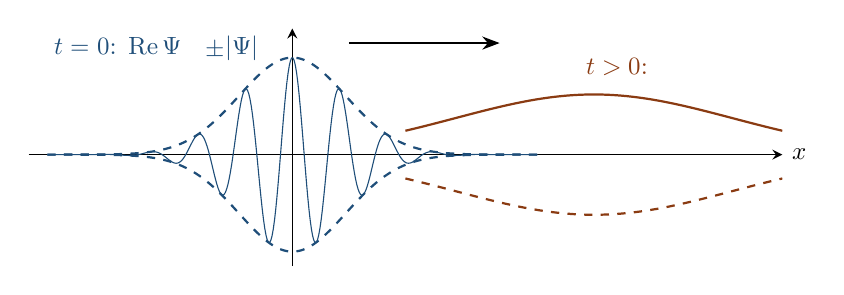
\begin{tikzpicture}
\begin{axis}[width=0.92\linewidth, height=4.6cm, axis lines=middle,
  xlabel={$x$}, ylabel={}, xmin=-7, xmax=13, ymin=-1.15, ymax=1.3,
  xtick=\empty, ytick=\empty, samples=400,
  xlabel style={at={(ticklabel* cs:1)}, anchor=west}]
  \addplot[domain=-6.5:6.5, accent, thin] {exp(-x^2/4)*cos(deg(5*x))};
  \addplot[domain=-6.5:6.5, accent, thick, dashed] {exp(-x^2/4)};
  \addplot[domain=-6.5:6.5, accent, thick, dashed] {-exp(-x^2/4)};
  \addplot[domain=3:13, keycol, thick] {0.62*exp(-(x-8)^2/(4*2.6^2/1))};
  \addplot[domain=3:13, keycol, thick, dashed] {-0.62*exp(-(x-8)^2/(4*2.6^2/1))};
  \node[font=\small, accent] at (axis cs:-3.6,1.1) {$t=0$: $\operatorname{Re}\Psi$ и $\pm|\Psi|$};
  \node[font=\small, keycol] at (axis cs:9.6,0.9) {$t>0$: огибающая};
  \draw[->, thick] (axis cs:1.5,1.15) -- (axis cs:5.5,1.15) node[midway, above, font=\small] {$v_{\text{гр}}$};
\end{axis}
\end{tikzpicture}
\caption{Гауссов волновой пакет: при $t=0$ показаны действительная часть $\Psi$ и огибающая
$\pm|\Psi|$; в более поздний момент пакет смещён на $v_{\text{гр}}t$ и расплылся
(амплитуда уменьшилась, ширина выросла; качественно).}
\label{fig:4:packet}
\end{figure}

\subsection{Вероятностная интерпретация: следствия}

\paragraph{Средние значения координаты.} Поскольку $|\Psi|^2$ — плотность вероятности,
\begin{equation}
  \avg{\vect r}=\int\vect r\,|\Psi|^2\dd V,\qquad \avg{f(\vect r)}=\int f(\vect r)|\Psi|^2\dd V .
\end{equation}

\paragraph{Распределение по импульсам.} Разложим $\Psi$ по плоским волнам (трёхмерное
обобщение~\eqref{eq:4:packet}):
\begin{equation}\label{eq:4:ap}
  \Psi(\vect r,t)=\int a(\vect p,t)\,\frac{\ee^{\ii\vect p\vect r/\hbar}}{(2\pi\hbar)^{3/2}}\,\dd^3p,
  \qquad
  a(\vect p,t)=\int\Psi(\vect r,t)\,\frac{\ee^{-\ii\vect p\vect r/\hbar}}{(2\pi\hbar)^{3/2}}\,\dd V .
\end{equation}
Согласно Борну, $|a(\vect p)|^2\dd^3p$ — вероятность того, что измерение импульса даст значение
в элементе $\dd^3p$ около $\vect p$. Равенство Парсеваля $\int|a|^2\dd^3p=\int|\Psi|^2\dd V=1$
обеспечивает согласованность нормировок. Это частный случай общего правила: коэффициенты
разложения $\Psi$ по собственным функциям оператора величины дают амплитуды вероятностей её
значений (\tref{t:05}).

\paragraph{Сохранение вероятности.} Вероятность найти частицу где-либо должна оставаться
равной 1. Из уравнения Шредингера (\tref{t:06}) следует локальный закон сохранения
\begin{equation}\label{eq:4:cont}
  \pdiff{\rho}{t}+\operatorname{div}\vect j=0,\qquad
  \vect j=\frac{\ii\hbar}{2m}\bigl(\Psi\nabla\Psi^*-\Psi^*\nabla\Psi\bigr)
  =\frac{\hbar}{m}\operatorname{Im}(\Psi^*\nabla\Psi),
\end{equation}
где $\vect j$ — \emph{плотность потока вероятности}. Для плоской волны~\eqref{eq:4:plane}
$\vect j=|A|^2\hbar\vect k/m=|A|^2\vect v$: поток = плотность $\times$ скорость, как для
классического пучка. Эта формула используется при вычислении коэффициентов отражения и
прохождения (\tref{t:07}).

\section{Математические выводы}

\begin{derivation}[label=der:4:group]{скорость движения волнового пакета}
\emph{Допущение:} $a(k)$ заметно отлична от нуля лишь в узкой окрестности $k_0$ ($\Delta k\ll k_0$),
и на рассматриваемых временах можно ограничиться линейным членом разложения
$\omega(k)\approx\omega_0+v_{\text{гр}}(k-k_0)$, где $\omega_0=\omega(k_0)$, $v_{\text{гр}}=(\dd\omega/\dd k)_{k_0}$.

Подставим в~\eqref{eq:4:packet} и вынесем множитель, не зависящий от $k$:
\begin{align*}
  \Psi(x,t)&\approx\frac{1}{\sqrt{2\pi}}\int a(k)\exp\bigl[\ii kx-\ii\omega_0t-\ii v_{\text{гр}}(k-k_0)t\bigr]\dd k\\
  &=\ee^{\ii(k_0v_{\text{гр}}-\omega_0)t}\cdot\frac{1}{\sqrt{2\pi}}\int a(k)\,\ee^{\ii k(x-v_{\text{гр}}t)}\dd k
  =\ee^{\ii(k_0v_{\text{гр}}-\omega_0)t}\,\Psi(x-v_{\text{гр}}t,\,0).
\end{align*}
Следовательно, $|\Psi(x,t)|^2=|\Psi(x-v_{\text{гр}}t,0)|^2$: распределение вероятности переносится
без изменения формы со скоростью $v_{\text{гр}}=\dd\omega/\dd k=\hbar k_0/m=p_0/m$. Учёт квадратичного
члена $\frac12\omega''(k-k_0)^2$, $\omega''=\hbar/m$, приводит к расплыванию~\eqref{eq:4:spread}.
\end{derivation}

\begin{derivation}[label=der:4:delta]{нормировка плоских волн на $\delta$-функцию}
Используем представление $\delta$-функции $\int_{-\infty}^{\infty}\ee^{\ii qx}\dd x=2\pi\,\delta(q)$.
Для одномерных волн $\psi_p(x)=A\ee^{\ii px/\hbar}$:
\[
  \int_{-\infty}^{\infty}\psi_{p'}^*(x)\psi_p(x)\,\dd x=|A|^2\int\ee^{\ii(p-p')x/\hbar}\dd x
  =|A|^2\,2\pi\,\delta\Bigl(\frac{p-p'}{\hbar}\Bigr)=|A|^2\,2\pi\hbar\,\delta(p-p').
\]
Условие $\int\psi_{p'}^*\psi_p\dd x=\delta(p-p')$ даёт $A=(2\pi\hbar)^{-1/2}$; в трёх измерениях
$A=(2\pi\hbar)^{-3/2}$. Волны с разными импульсами ортогональны; «нормировка» означает
полноту системы в смысле разложения~\eqref{eq:4:ap}.
\end{derivation}

\begin{derivation}[label=der:4:box]{нормировка в ящике с периодическими условиями}
Потребуем $\psi(x+L)=\psi(x)$ для $\psi=A\ee^{\ii kx}$: $\ee^{\ii kL}=1$ $\Rightarrow$
$k=2\pi n/L$, $n=0,\pm1,\dots$ Нормировка:
$\int_0^L|A|^2\dd x=|A|^2L=1$ $\Rightarrow$ $A=1/\sqrt L$. В трёх измерениях
$\psi_{\vect k}=V^{-1/2}\ee^{\ii\vect k\vect r}$, $\vect k=\frac{2\pi}{L}(n_x,n_y,n_z)$.
Число состояний в элементе $\dd^3k$ равно $V\dd^3k/(2\pi)^3$ (на одно значение $\vect k$
приходится объём $(2\pi/L)^3$), или $V\dd^3p/(2\pi\hbar)^3$ — это используется в статистике
(газ Ферми, \tref{t:17}; фазовый объём в бета-распаде, \tref{t:20}). При $L\to\infty$
физические результаты не зависят от $L$.
\end{derivation}

\begin{derivation}[label=der:4:current]{плотность потока для плоской волны}
Для $\Psi=A\ee^{\ii(\vect k\vect r-\omega t)}$ имеем $\nabla\Psi=\ii\vect k\Psi$,
$\nabla\Psi^*=-\ii\vect k\Psi^*$. Подставляя в~\eqref{eq:4:cont}:
\[
  \vect j=\frac{\ii\hbar}{2m}\bigl(\Psi(-\ii\vect k)\Psi^*-\Psi^*(\ii\vect k)\Psi\bigr)
  =\frac{\ii\hbar}{2m}(-2\ii\vect k)|A|^2=\frac{\hbar\vect k}{m}|A|^2=\vect v\,|A|^2 .
\]
Размерность при $[|A|^2]=\text{см}^{-3}$: $[\vect j]=\text{см}^{-2}\text{с}^{-1}$ — число частиц через
единичную площадку в единицу времени.
\end{derivation}

\section{Итоговые формулы}

\keyformula{\dd w=|\Psi(\vect r,t)|^2\dd V,\qquad \int|\Psi|^2\dd V=1}
 {$\Psi$ — волновая функция, $\dd w$ — вероятность нахождения в объёме $\dd V$.}
 {нерелятивистская частица, связанное (нормируемое) состояние.}
 {вероятности положения частицы, средние $\avg{f(\vect r)}=\int f|\Psi|^2\dd V$.}

\keyformula{\Psi_{\vect p}=A\exp\Bigl[\frac{\ii}{\hbar}(\vect p\vect r-Et)\Bigr],\qquad E=\frac{p^2}{2m}}
 {$\vect p$ — импульс, $E$ — энергия свободной частицы; $A=V^{-1/2}$ или $(2\pi\hbar)^{-3/2}$.}
 {свободная нерелятивистская частица с точно заданным импульсом.}
 {базис для разложения произвольных состояний; описание пучков частиц.}

\keyformula{v_{\text{ф}}=\frac{\omega}{k}=\frac v2,\qquad v_{\text{гр}}=\frac{\dd\omega}{\dd k}=\frac{p}{m}=v}
 {$\omega=\hbar k^2/2m$ — закон дисперсии волн де Бройля.}
 {свободная нерелятивистская частица; узкий пакет $\Delta k\ll k_0$.}
 {пакет движется со скоростью частицы; фазовая скорость физического смысла не имеет.}

\keyformula{\pdiff{\rho}{t}+\operatorname{div}\vect j=0,\qquad \vect j=\frac{\hbar}{m}\operatorname{Im}(\Psi^*\nabla\Psi)}
 {$\rho=|\Psi|^2$; $\vect j$ — плотность потока вероятности.}
 {действительный потенциал (нет поглощения).}
 {сохранение вероятности; коэффициенты отражения и прохождения.}

\section{Физическая интерпретация}

\textbf{Статистический характер.} Квантовая механика предсказывает не результат отдельного
измерения, а распределения вероятностей. Повторив опыт с одинаково приготовленными частицами
много раз, получаем распределение $|\Psi|^2$; отдельная частица регистрируется в одной точке.

\textbf{Волна и частица.} Интерференция электрона с самим собой (две щели) показывает, что
$\Psi$ описывает состояние одной частицы, а не ансамбля взаимодействующих частиц. Попытка
выяснить, через какую щель прошла частица, разрушает интерференцию: измерение меняет
состояние.

\textbf{Предельные случаи.} Плоская волна ($\Delta p=0$) полностью делокализована ($\Delta x=\infty$);
$\delta$-образный пакет ($\Delta x=0$) содержит все импульсы. Реальные состояния — промежуточные
пакеты, удовлетворяющие $\Delta x\Delta p\ge\hbar/2$. Для макрочастиц расплывание пренебрежимо, и
центр пакета движется по классической траектории.

\section{Что необходимо знать на экзамене}

\begin{examcheck}
\checkhead{Определения}
\begin{itemize}
 \item волновая функция, плотность вероятности, нормировка, стандартные условия;
 \item принцип суперпозиции и интерференционный член; фаза $\Psi$ не наблюдаема.
\end{itemize}
\checkhead{Формулы}
\begin{itemize}
 \item $\dd w=|\Psi|^2\dd V$; $\Psi_{\vect p}=A\,\ee^{\ii(\vect p\vect r-Et)/\hbar}$; $\omega=\hbar k^2/2m$;
 \item $v_{\text{ф}}=v/2$, $v_{\text{гр}}=v$; $\vect j=(\hbar/m)\operatorname{Im}(\Psi^*\nabla\Psi)$; $|a(\vect p)|^2$ — распределение по импульсам.
\end{itemize}
\checkhead{Выводы}
\begin{itemize}
 \item групповая скорость пакета равна скорости частицы;
 \item нормировка плоской волны (в ящике и на $\delta$-функцию); поток для плоской волны.
\end{itemize}
\checkhead{Интерпретации}
\begin{itemize}
 \item почему $\ee^{\ii kx}$, а не $\cos kx$; почему плоская волна не нормируема;
 \item опыт с двумя щелями и поштучной регистрацией; расплывание пакета и его оценки.
\end{itemize}
\end{examcheck}

% ======================================================================
\chapter[Операторы. Собственные функции и собственные значения]%
        {Квантово-механические операторы. Собственные функции и значения}
\label{t:05}
% ======================================================================

\begin{qbox}
\textbf{Билет 5.} Понятие о квантово-механических операторах. Операторы координаты,
импульса, потенциальной и кинетической энергии системы, гамильтониан. Собственные функции и
собственные значения операторов.
\end{qbox}

\section{Содержание билета}

\textbf{Подтемы:}
\begin{enumerate}
 \item оператор, линейность, эрмитовость; связь операторов с наблюдаемыми величинами;
 \item операторы координаты, импульса, кинетической и потенциальной энергии, гамильтониан (для одной частицы и системы);
 \item задача на собственные значения; спектр (дискретный и непрерывный), вырождение;
 \item свойства собственных функций эрмитовых операторов: действительность собственных значений,
       ортогональность, полнота; вероятности результатов измерений и средние;
 \item коммутаторы, одновременная измеримость, соотношение неопределённостей.
\end{enumerate}

\textbf{Необходимые понятия:} волновая функция и интерпретация Борна (\tref{t:04});
скалярное произведение функций; интегрирование по частям; ряд и интеграл Фурье.

\section{Определения и физические принципы}

\begin{definition}[оператор]
\emph{Оператор} $\op A$ — правило, сопоставляющее функции $\psi$ другую функцию $\varphi=\op A\psi$.
Оператор \emph{линеен}, если $\op A(c_1\psi_1+c_2\psi_2)=c_1\op A\psi_1+c_2\op A\psi_2$.
Примеры: умножение на функцию $f(x)$, дифференцирование $\dd/\dd x$.
\end{definition}

\begin{definition}[эрмитов оператор]
Скалярное произведение $\langle\varphi|\psi\rangle=\int\varphi^*\psi\,\dd V$. Оператор $\op A$
\emph{эрмитов} (самосопряжён), если для любых допустимых $\varphi,\psi$
\begin{equation}\label{eq:5:herm}
  \int\varphi^*\,(\op A\psi)\,\dd V=\int(\op A\varphi)^*\,\psi\,\dd V .
\end{equation}
\end{definition}

\begin{definition}[собственные функции и значения]
Если $\op A\psi_a=a\,\psi_a$, где $a$ — число, а $\psi_a$ удовлетворяет стандартным условиям,
то $\psi_a$ — \emph{собственная функция}, $a$ — \emph{собственное значение}. Множество собственных
значений — \emph{спектр} оператора (дискретный, непрерывный или смешанный). Если одному $a$
отвечают $g>1$ линейно независимых собственных функций, значение $a$ \emph{вырождено} с
кратностью $g$.
\end{definition}

\begin{principle}{Постулаты, связывающие операторы с измерениями}
\begin{enumerate}[leftmargin=1.4em]
 \item Каждой физической величине $A$ сопоставляется линейный эрмитов оператор $\op A$.
 \item При измерении $A$ могут получиться только собственные значения $a_n$ оператора $\op A$.
 \item Если $\psi=\sum_nc_n\psi_n$ — разложение состояния по нормированным собственным функциям,
       то вероятность получить $a_n$ равна $|c_n|^2$, где $c_n=\int\psi_n^*\psi\,\dd V$.
 \item Среднее значение величины в состоянии $\psi$:
       \begin{equation}\label{eq:5:mean}
         \avg A=\int\psi^*\op A\psi\,\dd V .
       \end{equation}
 \item После измерения, давшего $a_n$, система оказывается в состоянии $\psi_n$ (для невырожденного $a_n$).
\end{enumerate}
\end{principle}

\emph{Физический смысл.} В состоянии, являющемся собственной функцией $\op A$, величина $A$ имеет
точное значение: разброс результатов $\Delta A=0$. В общем состоянии $A$ не имеет определённого
значения, и квантовая механика даёт лишь распределение вероятностей. Эрмитовость нужна для
того, чтобы результаты измерений (собственные значения) и средние были действительными.

\section{Основная теория}

\subsection{Почему величинам сопоставляются операторы}

В классической механике состояние — точка фазового пространства $(x,p)$, и любая величина —
функция $A(x,p)$. В квантовой механике состояние — волновая функция, и вопрос «каково значение
$p$ в состоянии $\psi$?» в общем случае не имеет ответа (соотношение неопределённостей). Можно
спрашивать лишь о распределении результатов. Оказывается, всю информацию о распределении
величины удобно закодировать оператором: его собственные значения — возможные результаты,
собственные функции — состояния с определённым значением, а формула~\eqref{eq:5:mean} даёт среднее.

\subsection{Основные операторы}

\paragraph{Координата.} Поскольку $|\psi(\vect r)|^2$ — плотность вероятности координаты,
$\avg{\vect r}=\int\psi^*\vect r\psi\,\dd V$, т.\,е. $\op{\vect r}=\vect r$ — оператор умножения на
координату. Аналогично $\op U=U(\vect r)$ — оператор потенциальной энергии (умножение на функцию).

\paragraph{Импульс.} Плоская волна $\ee^{\ii px/\hbar}$ — состояние с определённым импульсом $p$;
она должна быть собственной функцией $\op p_x$ с собственным значением $p$. Этому требованию
удовлетворяет дифференциальный оператор
\begin{equation}\label{eq:5:p}
  \op p_x=-\ii\hbar\pdiff{}{x},\qquad \op{\vect p}=-\ii\hbar\nabla:\qquad
  -\ii\hbar\pdiff{}{x}\ee^{\ii px/\hbar}=p\,\ee^{\ii px/\hbar}.
\end{equation}
Строгое обоснование: среднее импульса, вычисленное через распределение $|a(p)|^2$ (\tref{t:04}),
совпадает с $\int\psi^*(-\ii\hbar\,\dd/\dd x)\psi\,\dd x$ (вывод~\ref{der:5:pmean}).

\paragraph{Кинетическая энергия и гамильтониан.} Операторы функций от импульса строятся
подстановкой $\vect p\to\op{\vect p}$:
\begin{equation}\label{eq:5:T}
  \op T=\frac{\op{\vect p}^{\,2}}{2m}=-\frac{\hbar^2}{2m}\nabla^2=
  -\frac{\hbar^2}{2m}\Bigl(\pdiff{^2}{x^2}+\pdiff{^2}{y^2}+\pdiff{^2}{z^2}\Bigr).
\end{equation}
Гамильтониан — оператор полной энергии:
\begin{equation}\label{eq:5:H}
  \op H=\op T+\op U=-\frac{\hbar^2}{2m}\nabla^2+U(\vect r).
\end{equation}
Для системы $N$ частиц с массами $m_i$, взаимодействующих между собой и находящихся во внешнем поле:
\begin{equation}\label{eq:5:HN}
  \op H=\sum_{i=1}^{N}\Bigl(-\frac{\hbar^2}{2m_i}\nabla_i^2\Bigr)+U(\vect r_1,\dots,\vect r_N),
\end{equation}
где $\nabla_i$ действует на координаты $i$-й частицы. Например, для атома гелия (ядро
неподвижно) $U=-2e^2/r_1-2e^2/r_2+e^2/|\vect r_1-\vect r_2|$.

\begin{remark}[Правило соответствия]
Переход $A(\vect r,\vect p)\to\op A=A(\op{\vect r},\op{\vect p})$ однозначен, если в $A$ нет произведений
некоммутирующих множителей вида $xp_x$. В общем случае требуется симметризация, например
$xp_x\to\frac12(\op x\op p_x+\op p_x\op x)$, чтобы оператор был эрмитовым.
\end{remark}

\subsection{Свойства собственных функций эрмитовых операторов}

\begin{enumerate}
 \item \textbf{Собственные значения действительны} (вывод~\ref{der:5:real}).
 \item \textbf{Собственные функции, отвечающие разным собственным значениям, ортогональны}
       (вывод~\ref{der:5:orth}); в случае вырождения их можно выбрать ортогональными.
 \item \textbf{Полнота:} любую допустимую функцию можно разложить по собственным функциям
       эрмитова оператора (утверждение без доказательства):
       \begin{equation}\label{eq:5:expand}
         \psi=\sum_nc_n\psi_n+\int c(a)\psi_a\,\dd a,\qquad c_n=\int\psi_n^*\psi\,\dd V .
       \end{equation}
       Для нормированного $\psi$ $\sum|c_n|^2+\int|c(a)|^2\dd a=1$ — сумма вероятностей всех исходов.
\end{enumerate}
Из разложения следует, что среднее~\eqref{eq:5:mean} равно $\sum_na_n|c_n|^2$ — обычному
статистическому среднему (вывод~\ref{der:5:avg}).

\subsection{Примеры задач на собственные значения}

\textbf{Импульс} ($-\ii\hbar\psi'=p\psi$): $\psi_p=C\ee^{\ii px/\hbar}$; ограниченность при
$x\to\pm\infty$ требует действительного $p$; спектр непрерывный, $-\infty<p<\infty$; функции
нормируются на $\delta$-функцию (\tref{t:04}).

\textbf{Координата} ($x\psi=x_0\psi$): $\psi_{x_0}=\delta(x-x_0)$ — состояние, локализованное в точке;
спектр непрерывный.

\textbf{Проекция момента импульса} $\op L_z=-\ii\hbar\,\partial/\partial\varphi$: условие однозначности
$\psi(\varphi+2\pi)=\psi(\varphi)$ делает спектр \emph{дискретным}: $L_z=m\hbar$ (\tref{t:09}).
Этот пример показывает, что дискретность возникает из граничных условий.

\textbf{Гамильтониан} ($\op H\psi=E\psi$) — стационарное уравнение Шредингера (\tref{t:06}):
для связанных состояний спектр дискретен (яма, осциллятор, атом), для инфинитного
движения — непрерывен.

\subsection{Коммутаторы и одновременная измеримость}

Коммутатор $[\op A,\op B]=\op A\op B-\op B\op A$. Основное соотношение (вывод~\ref{der:5:comm})
\begin{equation}\label{eq:5:xp}
  [\op x,\op p_x]=\ii\hbar,\qquad [\op x,\op p_y]=0,\qquad [\op p_x,\op p_y]=0 .
\end{equation}
\textbf{Теорема.} Две величины имеют общую полную систему собственных функций (одновременно
измеримы, могут иметь одновременно точные значения) тогда и только тогда, когда их операторы
коммутируют. Если $[\op A,\op B]\neq0$, справедливо обобщённое соотношение неопределённостей
(вывод~\ref{der:5:robertson})
\begin{equation}\label{eq:5:rob}
  \Delta A\,\Delta B\ge\frac12\bigl|\avg{[\op A,\op B]}\bigr| ,
\end{equation}
которое для $x$ и $p_x$ даёт $\Delta x\,\Delta p_x\ge\hbar/2$ (\tref{t:02}).
Величина, оператор которой коммутирует с $\op H$ (и не зависит явно от времени), сохраняется:
её среднее не меняется со временем, а распределение вероятностей стационарно.

\section{Математические выводы}

\begin{derivation}[label=der:5:pherm]{эрмитовость оператора импульса}
Пусть $\varphi,\psi\to0$ при $x\to\pm\infty$ (нормируемые функции). Интегрируя по частям:
\[
  \int_{-\infty}^{\infty}\varphi^*\Bigl(-\ii\hbar\diff{\psi}{x}\Bigr)\dd x
  =-\ii\hbar\bigl[\varphi^*\psi\bigr]_{-\infty}^{\infty}+\ii\hbar\int\diff{\varphi^*}{x}\psi\,\dd x
  =\int\Bigl(-\ii\hbar\diff{\varphi}{x}\Bigr)^{\!*}\psi\,\dd x .
\]
Внеинтегральный член равен нулю, а $\ii\hbar\,\dd\varphi^*/\dd x=(-\ii\hbar\,\dd\varphi/\dd x)^*$.
Условие~\eqref{eq:5:herm} выполнено. Заметим: оператор $\dd/\dd x$ без множителя $\ii$ эрмитовым
не является (он антиэрмитов), поэтому множитель $-\ii$ в $\op p$ необходим. Эрмитовость $\op T$
следует из двукратного интегрирования по частям, $\op U$ — очевидна (умножение на
действительную функцию), следовательно, эрмитов и $\op H$.
\end{derivation}

\begin{derivation}[label=der:5:real]{собственные значения эрмитова оператора действительны}
Пусть $\op A\psi=a\psi$, $\int|\psi|^2\dd V=1$. Положим в~\eqref{eq:5:herm} $\varphi=\psi$:
\[
  \int\psi^*\op A\psi\,\dd V=a\int|\psi|^2\dd V=a,\qquad
  \int(\op A\psi)^*\psi\,\dd V=a^*\int|\psi|^2\dd V=a^* .
\]
Из эрмитовости левые части равны, значит $a=a^*$.
\end{derivation}

\begin{derivation}[label=der:5:orth]{ортогональность собственных функций}
Пусть $\op A\psi_1=a_1\psi_1$, $\op A\psi_2=a_2\psi_2$, $a_1\neq a_2$ (оба действительны).
Из~\eqref{eq:5:herm} с $\varphi=\psi_1$, $\psi=\psi_2$:
\[
  \int\psi_1^*\op A\psi_2\,\dd V=a_2\int\psi_1^*\psi_2\,\dd V,\qquad
  \int(\op A\psi_1)^*\psi_2\,\dd V=a_1\int\psi_1^*\psi_2\,\dd V .
\]
Вычитая: $(a_2-a_1)\int\psi_1^*\psi_2\,\dd V=0$, а так как $a_1\neq a_2$, то $\int\psi_1^*\psi_2\,\dd V=0$.
\end{derivation}

\begin{derivation}[label=der:5:avg]{среднее значение как статистическое среднее}
Подставим $\psi=\sum_nc_n\psi_n$ в~\eqref{eq:5:mean} (дискретный спектр, $\int\psi_m^*\psi_n=\delta_{mn}$):
\[
  \avg A=\int\Bigl(\sum_mc_m^*\psi_m^*\Bigr)\op A\Bigl(\sum_nc_n\psi_n\Bigr)\dd V
  =\sum_{m,n}c_m^*c_n\,a_n\int\psi_m^*\psi_n\,\dd V=\sum_n a_n|c_n|^2 .
\]
Это среднее значение случайной величины, принимающей значения $a_n$ с вероятностями $|c_n|^2$.
Нормировка $\psi$ даёт $\sum|c_n|^2=1$.
\end{derivation}

\begin{derivation}[label=der:5:pmean]{среднее импульса: обоснование $\op p=-\ii\hbar\,\dd/\dd x$}
По Борну, распределение импульса задаётся $|a(p)|^2$, где $\psi(x)=\int a(p)\frac{\ee^{\ii px/\hbar}}{\sqrt{2\pi\hbar}}\dd p$.
Подействуем на $\psi$ оператором $-\ii\hbar\,\dd/\dd x$: дифференцирование под интегралом даёт
множитель $p$:
\[
  -\ii\hbar\diff{\psi}{x}=\int p\,a(p)\frac{\ee^{\ii px/\hbar}}{\sqrt{2\pi\hbar}}\dd p .
\]
Тогда, используя $\int\ee^{\ii(p-p')x/\hbar}\dd x=2\pi\hbar\,\delta(p-p')$,
\[
  \int\psi^*\Bigl(-\ii\hbar\diff{\psi}{x}\Bigr)\dd x
  =\iint a^*(p')\,p\,a(p)\Bigl[\int\frac{\ee^{\ii(p-p')x/\hbar}}{2\pi\hbar}\dd x\Bigr]\dd p\,\dd p'
  =\int p\,|a(p)|^2\dd p=\avg p .
\]
Таким образом, формула~\eqref{eq:5:mean} с $\op p=-\ii\hbar\,\dd/\dd x$ даёт правильное среднее,
вычисляемое непосредственно в координатном представлении.
\end{derivation}

\begin{derivation}[label=der:5:comm]{коммутатор $[\op x,\op p_x]=\ii\hbar$}
Подействуем коммутатором на произвольную функцию $\psi(x)$:
\[
  [\op x,\op p_x]\psi=x\Bigl(-\ii\hbar\diff{\psi}{x}\Bigr)-\Bigl(-\ii\hbar\diff{}{x}\Bigr)(x\psi)
  =-\ii\hbar x\psi'+\ii\hbar(\psi+x\psi')=\ii\hbar\psi .
\]
Так как $\psi$ произвольна, $[\op x,\op p_x]=\ii\hbar$. Для $x$ и $p_y$: $\partial(x\psi)/\partial y=x\,\partial\psi/\partial y$,
поэтому $[\op x,\op p_y]=0$. Производные по разным переменным коммутируют, поэтому $[\op p_x,\op p_y]=0$.
\end{derivation}

\begin{derivation}[label=der:5:robertson]{соотношение неопределённостей $\Delta x\,\Delta p_x\ge\hbar/2$}
\emph{Допущение:} $\psi$ нормирована и убывает на бесконечности. Без ограничения общности
$\avg x=0$, $\avg{p_x}=0$ (иначе сделаем сдвиг $x\to x-\avg x$ и умножим $\psi$ на
$\ee^{-\ii\avg{p}x/\hbar}$; это не меняет $\Delta x$, $\Delta p$). Тогда $(\Delta x)^2=\avg{x^2}$,
$(\Delta p)^2=\avg{p^2}$.

Рассмотрим при действительном $\alpha$ неотрицательный интеграл
\[
  I(\alpha)=\int_{-\infty}^{\infty}\Bigl|\alpha x\psi+\hbar\diff{\psi}{x}\Bigr|^2\dd x\ge0 .
\]
Раскроем модуль:
\[
  I(\alpha)=\alpha^2\int x^2|\psi|^2\dd x+\alpha\hbar\int x\Bigl(\psi^*\diff{\psi}{x}+\psi\diff{\psi^*}{x}\Bigr)\dd x
  +\hbar^2\int\Bigl|\diff{\psi}{x}\Bigr|^2\dd x .
\]
\emph{Первый член:} $\alpha^2\avg{x^2}$.
\emph{Второй:} $\psi^*\psi'+\psi\psi^{*\prime}=\dd|\psi|^2/\dd x$; по частям
$\int x\,\dd|\psi|^2=[x|\psi|^2]-\int|\psi|^2\dd x=-1$. Итого $-\alpha\hbar$.
\emph{Третий:} по частям $\int|\psi'|^2\dd x=-\int\psi^*\psi''\dd x=\avg{p^2}/\hbar^2$, т.\,е.
третий член равен $\avg{p^2}$. Следовательно,
\[
  I(\alpha)=\avg{x^2}\alpha^2-\hbar\alpha+\avg{p^2}\ge0\quad\text{при всех }\alpha .
\]
Квадратный трёхчлен неотрицателен при всех $\alpha$, только если его дискриминант
неположителен: $\hbar^2-4\avg{x^2}\avg{p^2}\le0$, т.\,е.
\[
  \Delta x\,\Delta p_x\ge\frac{\hbar}{2}.
\]
Равенство достигается, если при некотором $\alpha$ $\alpha x\psi+\hbar\psi'=0$, т.\,е. $\psi\propto\ee^{-\alpha x^2/2\hbar}$ —
гауссов пакет. Для произвольных эрмитовых операторов аналогичное рассуждение даёт~\eqref{eq:5:rob}.
\end{derivation}

\section{Итоговые формулы}

\keyformula{\op{\vect r}=\vect r,\qquad \op{\vect p}=-\ii\hbar\nabla,\qquad \op T=-\frac{\hbar^2}{2m}\nabla^2,\qquad \op U=U(\vect r)}
 {$\nabla$ — оператор градиента, $\nabla^2$ — лапласиан.}
 {координатное представление, нерелятивистская частица без спина.}
 {построение операторов любых величин $A(\vect r,\vect p)$.}

\keyformula{\op H=\sum_i\Bigl(-\frac{\hbar^2}{2m_i}\nabla_i^2\Bigr)+U(\vect r_1,\dots,\vect r_N)}
 {$m_i$, $\nabla_i$ — масса и градиент по координатам $i$-й частицы; $U$ — полная потенциальная энергия.}
 {нерелятивистская система без спин-зависящих сил и магнитного поля.}
 {гамильтониан системы — входит в уравнение Шредингера.}

\keyformula{\op A\psi_n=a_n\psi_n,\qquad w_n=|c_n|^2,\ c_n=\int\psi_n^*\psi\,\dd V,\qquad \avg A=\int\psi^*\op A\psi\,\dd V}
 {$a_n$ — собственные значения, $\psi_n$ — ортонормированные собственные функции, $w_n$ — вероятность результата $a_n$.}
 {эрмитов оператор, дискретный спектр (для непрерывного — суммы заменяются интегралами).}
 {возможные результаты измерения и их вероятности; средние значения.}

\keyformula{[\op x,\op p_x]=\ii\hbar,\qquad \Delta A\,\Delta B\ge\tfrac12|\avg{[\op A,\op B]}|}
 {$[\op A,\op B]=\op A\op B-\op B\op A$, $\Delta$ — среднеквадратичные отклонения.}
 {любое состояние, для которого определены средние.}
 {критерий одновременной измеримости; соотношения неопределённостей.}

\section{Физическая интерпретация}

\textbf{Дискретность — следствие граничных условий.} Сами по себе дифференциальные уравнения на
собственные значения имеют решения при любых $a$; требование однозначности, конечности,
нормируемости отбирает дискретный набор (момент импульса, связанные состояния). Непрерывный
спектр соответствует инфинитному движению.

\textbf{Измерение.} Если состояние — собственная функция $\op A$, измерение $A$ даёт заведомо
одно значение. В суперпозиции результат случаен; повторное немедленное измерение даёт тот же
результат (состояние после измерения — собственная функция).

\textbf{Некоммутирующие величины.} Пары $x$ и $p_x$, $L_x$ и $L_y$ (\tref{t:09}) не могут иметь
одновременно точных значений. Коммутирующие наборы ($\op H,\op L^2,\op L_z$ для атома водорода)
дают квантовые числа, классифицирующие состояния (\tref{t:10}).

\section{Что необходимо знать на экзамене}

\begin{examcheck}
\checkhead{Определения}
\begin{itemize}
 \item линейный и эрмитов оператор; собственные функции и значения; спектр; вырождение;
 \item постулаты: результаты измерений — собственные значения; вероятности $|c_n|^2$; среднее $\int\psi^*\op A\psi$.
\end{itemize}
\checkhead{Формулы}
\begin{itemize}
 \item $\op x=x$, $\op p_x=-\ii\hbar\,\partial_x$, $\op T=-\hbar^2\nabla^2/2m$, $\op H=\op T+U$; гамильтониан системы;
 \item $[\op x,\op p_x]=\ii\hbar$; $\Delta A\Delta B\ge\frac12|\avg{[\op A,\op B]}|$.
\end{itemize}
\checkhead{Выводы}
\begin{itemize}
 \item эрмитовость $\op p$; действительность собственных значений; ортогональность собственных функций;
 \item $\avg A=\sum a_n|c_n|^2$; коммутатор $[x,p]$; доказательство $\Delta x\Delta p\ge\hbar/2$.
\end{itemize}
\checkhead{Интерпретации}
\begin{itemize}
 \item почему наблюдаемым соответствуют эрмитовы операторы; откуда берётся дискретность спектра;
 \item физический смысл коммутации; сохраняющиеся величины ($[\op A,\op H]=0$).
\end{itemize}
\end{examcheck}

% ======================================================================
\chapter[Уравнение Шредингера. Бесконечно глубокая яма]%
        {Уравнение Шредингера. Бесконечно глубокая потенциальная яма}
\label{t:06}
% ======================================================================

\begin{qbox}
\textbf{Билет 6.} Уравнение Шредингера. Волновые функции и уровни энергии стационарных
состояний одномерной потенциальной ямы бесконечной глубины.
\end{qbox}

\section{Содержание билета}

\textbf{Подтемы:}
\begin{enumerate}
 \item временно́е уравнение Шредингера: обоснование, свойства (линейность, первый порядок по времени, сохранение нормировки);
 \item стационарные состояния; стационарное уравнение Шредингера как задача на собственные значения $\op H$;
 \item граничные условия для волновой функции;
 \item одномерная бесконечно глубокая яма: уровни энергии, нормированные волновые функции, их свойства;
 \item обобщение на трёхмерный ящик, вырождение.
\end{enumerate}

\textbf{Необходимые понятия:} волновая функция и плотность вероятности (\tref{t:04});
операторы $\op{\vect p}$, $\op H$ и задача на собственные значения (\tref{t:05}); решение
линейного ОДУ с постоянными коэффициентами.

\section{Определения и физические принципы}

\begin{principle}{Уравнение Шредингера (1926)}
Эволюция волновой функции во времени определяется уравнением
\begin{equation}\label{eq:6:tdse}
  \ii\hbar\pdiff{\Psi(\vect r,t)}{t}=\op H\Psi(\vect r,t),\qquad
  \op H=-\frac{\hbar^2}{2m}\nabla^2+U(\vect r,t).
\end{equation}
\end{principle}

\emph{Статус.} Уравнение Шредингера — постулат квантовой механики; его нельзя вывести из
классической физики, но можно обосновать (см. ниже) и проверить опытом. Его роль аналогична
роли уравнений Ньютона в механике или уравнений Максвелла в электродинамике.

\begin{definition}[стационарное состояние]
Состояние с определённым значением энергии $E$. Его волновая функция имеет вид
\begin{equation}\label{eq:6:stat}
  \Psi(\vect r,t)=\psi(\vect r)\,\ee^{-\ii Et/\hbar},
\end{equation}
а $\psi$ удовлетворяет \emph{стационарному уравнению Шредингера}
\begin{equation}\label{eq:6:sse}
  \op H\psi=E\psi,\qquad -\frac{\hbar^2}{2m}\nabla^2\psi+U(\vect r)\psi=E\psi .
\end{equation}
\end{definition}

\emph{Физический смысл.} В стационарном состоянии плотность вероятности $|\Psi|^2=|\psi|^2$ и
средние всех величин, не зависящих явно от времени, постоянны. Именно такие состояния —
«стационарные орбиты» Бора — дают дискретные уровни энергии атомов.

\begin{definition}[потенциальная яма бесконечной глубины]
Одномерная модель частицы, запертой между непроницаемыми стенками:
$U(x)=0$ при $0<x<a$, $U(x)=+\infty$ при $x\le0$ и $x\ge a$.
\end{definition}

\emph{Область применимости модели:} электрон в тонкой плёнке, квантовой яме полупроводниковой
гетероструктуры, в длинной сопряжённой молекуле; нуклон в ядре (грубо). Модель годится,
когда энергия частицы много меньше высоты реальных стенок.

\section{Основная теория}

\subsection{Обоснование уравнения Шредингера}

Требуется линейное уравнение (чтобы выполнялся принцип суперпозиции), первого порядка по
времени (чтобы состояние в момент $t$ определялось только $\Psi(\vect r,0)$), решением которого
для свободной частицы является волна де Бройля $\Psi=A\ee^{\ii(\vect p\vect r-Et)/\hbar}$ с
$E=p^2/2m$. Для неё
\[
  \ii\hbar\pdiff{\Psi}{t}=E\Psi,\qquad -\ii\hbar\nabla\Psi=\vect p\Psi,\qquad
  -\hbar^2\nabla^2\Psi=p^2\Psi .
\]
Соотношение $E=p^2/2m$ превращается в уравнение $\ii\hbar\,\partial_t\Psi=-\frac{\hbar^2}{2m}\nabla^2\Psi$.
Обобщение на частицу в поле получается заменой $E=p^2/2m+U$, что даёт~\eqref{eq:6:tdse}.
Итак, уравнение Шредингера — операторная запись закона сохранения энергии
$E=p^2/2m+U$ с заменами $E\to\ii\hbar\,\partial_t$, $\vect p\to-\ii\hbar\nabla$.

\subsection{Свойства уравнения}

\begin{enumerate}
 \item \textbf{Линейность и однородность} — сумма решений есть решение (принцип суперпозиции).
 \item \textbf{Первый порядок по $t$} — задание $\Psi(\vect r,0)$ однозначно определяет $\Psi(\vect r,t)$:
       квантовая механика детерминистична на уровне волновой функции; случайны лишь результаты измерений.
 \item \textbf{Комплексность} — уравнение содержит $\ii$, поэтому $\Psi$ обязательно комплексна
       (действительное решение не может описывать движение).
 \item \textbf{Сохранение нормировки:} при действительном $U$ выполняется уравнение непрерывности
       $\partial_t|\Psi|^2+\operatorname{div}\vect j=0$ (вывод~\ref{der:6:cont}), и
       $\int|\Psi|^2\dd V$ не зависит от $t$.
\end{enumerate}

\subsection{Стационарные состояния и общее решение}

Если $U$ не зависит от времени, переменные разделяются (вывод~\ref{der:6:sep}), и решения
вида~\eqref{eq:6:stat} существуют для собственных значений $E_n$ оператора $\op H$. Общее
решение — суперпозиция стационарных:
\begin{equation}\label{eq:6:gen}
  \Psi(\vect r,t)=\sum_nc_n\psi_n(\vect r)\,\ee^{-\ii E_nt/\hbar},\qquad
  c_n=\int\psi_n^*(\vect r)\Psi(\vect r,0)\,\dd V .
\end{equation}
Коэффициенты $|c_n|^2$ — вероятности значений энергии $E_n$ — не меняются со временем
(энергия сохраняется), а $|\Psi|^2$ содержит интерференционные члены, осциллирующие с
частотами $(E_n-E_m)/\hbar$ — «боровскими частотами» переходов.

\subsection{Граничные условия}

Стационарное уравнение~\eqref{eq:6:sse} — уравнение второго порядка. Если $U(x)$ имеет конечный
скачок в точке $x_0$, то, интегрируя~\eqref{eq:6:sse} по малому интервалу $(x_0-\varepsilon,x_0+\varepsilon)$, получаем
\[
  \psi'(x_0+\varepsilon)-\psi'(x_0-\varepsilon)=\frac{2m}{\hbar^2}\int_{x_0-\varepsilon}^{x_0+\varepsilon}(U-E)\psi\,\dd x\xrightarrow[\varepsilon\to0]{}0 ,
\]
поскольку подынтегральная функция ограничена. Следовательно, на конечном скачке потенциала
\emph{непрерывны $\psi$ и $\psi'$}. Если же $U=+\infty$ в некоторой области, частица туда
проникнуть не может: $\psi=0$ в этой области, а на её границе $\psi=0$; производная $\psi'$
при этом испытывает скачок (интеграл от $U\psi$ не стремится к нулю).

\subsection{Бесконечно глубокая яма}

Внутри ямы ($0<x<a$) $U=0$, и уравнение~\eqref{eq:6:sse} принимает вид $\psi''+k^2\psi=0$, где
$k^2=2mE/\hbar^2$. С граничными условиями $\psi(0)=\psi(a)=0$ получаем (вывод~\ref{der:6:well})
\begin{equation}\label{eq:6:wellres}
  E_n=\frac{\pi^2\hbar^2}{2ma^2}\,n^2,\qquad
  \psi_n(x)=\sqrt{\frac{2}{a}}\sin\frac{\pi nx}{a},\qquad n=1,2,3,\dots
\end{equation}
Уровни, волновые функции и плотности вероятности для $n=1,2,3$ показаны на рис.~\ref{fig:6:well}.

\begin{figure}[htbp]
\centering
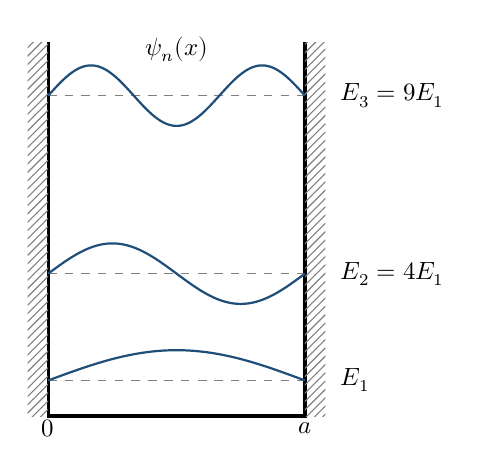
\begin{tikzpicture}
\begin{axis}[width=0.48\linewidth, height=6.6cm, axis lines=none,
  xmin=-0.15, xmax=1.15, ymin=-0.3, ymax=10.8, samples=120, clip=false]
  \addplot[very thick] coordinates {(0,10.5) (0,0) (1,0) (1,10.5)};
  \fill[pattern=north east lines, pattern color=gray] (axis cs:-0.08,0) rectangle (axis cs:0,10.5);
  \fill[pattern=north east lines, pattern color=gray] (axis cs:1,0) rectangle (axis cs:1.08,10.5);
  \foreach \n in {1,2,3} {
     \addplot[gray, dashed, domain=0:1] {\n*\n};
     \addplot[accent, thick, domain=0:1] {\n*\n + 0.85*sin(deg(pi*\n*x))};
  }
  \node[font=\small, anchor=west] at (axis cs:1.1,1) {$E_1$};
  \node[font=\small, anchor=west] at (axis cs:1.1,4) {$E_2=4E_1$};
  \node[font=\small, anchor=west] at (axis cs:1.1,9) {$E_3=9E_1$};
  \node[font=\small] at (axis cs:0,-0.35) {$0$};
  \node[font=\small] at (axis cs:1,-0.35) {$a$};
  \node[font=\small] at (axis cs:0.5,10.3) {$\psi_n(x)$};
\end{axis}
\end{tikzpicture}\hfill
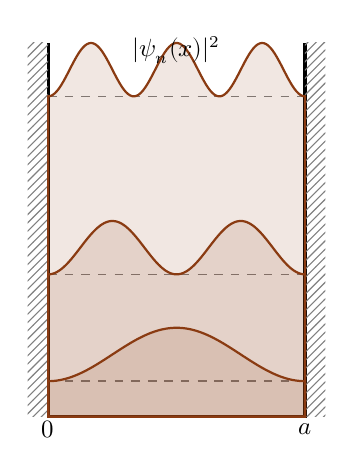
\begin{tikzpicture}
\begin{axis}[width=0.48\linewidth, height=6.6cm, axis lines=none,
  xmin=-0.15, xmax=1.15, ymin=-0.3, ymax=10.8, samples=120, clip=false]
  \addplot[very thick] coordinates {(0,10.5) (0,0) (1,0) (1,10.5)};
  \fill[pattern=north east lines, pattern color=gray] (axis cs:-0.08,0) rectangle (axis cs:0,10.5);
  \fill[pattern=north east lines, pattern color=gray] (axis cs:1,0) rectangle (axis cs:1.08,10.5);
  \foreach \n in {1,2,3} {
     \addplot[gray, dashed, domain=0:1] {\n*\n};
     \addplot[keycol, thick, domain=0:1, fill=keycol, fill opacity=0.12] {\n*\n + 1.5*(sin(deg(pi*\n*x)))^2} \closedcycle;
  }
  \node[font=\small] at (axis cs:0,-0.35) {$0$};
  \node[font=\small] at (axis cs:1,-0.35) {$a$};
  \node[font=\small] at (axis cs:0.5,10.3) {$|\psi_n(x)|^2$};
\end{axis}
\end{tikzpicture}
\caption{Бесконечно глубокая яма: уровни энергии $E_n\propto n^2$ (штриховые линии),
волновые функции $\psi_n$ (слева) и плотности вероятности $|\psi_n|^2$ (справа) для $n=1,2,3$.
Функция $\psi_n$ имеет $n-1$ узел внутри ямы.}
\label{fig:6:well}
\end{figure}

\paragraph{Свойства решения.}
\begin{enumerate}
 \item \textbf{Дискретность} спектра — следствие условия обращения $\psi$ в нуль на обеих стенках:
       на ширине ямы должно укладываться целое число полуволн де Бройля, $a=n\lambda_n/2$.
 \item \textbf{Энергия нулевых колебаний.} Наименьшая энергия $E_1=\pi^2\hbar^2/2ma^2>0$:
       состояние с $E=0$ ($\psi\equiv0$) не нормируемо. Согласие с соотношением
       неопределённостей: $\Delta x\sim a$, $p\gtrsim\hbar/a$, $E\gtrsim\hbar^2/ma^2$.
 \item \textbf{Узлы.} $\psi_n$ имеет $n-1$ нулей внутри ямы (осцилляционная теорема: $n$-е по
       порядку состояние одномерной задачи имеет $n-1$ узлов).
 \item \textbf{Чётность.} Относительно центра ямы $x=a/2$ функции с нечётными $n$ чётны, с
       чётными $n$ — нечётны (следствие симметрии $U(x)$).
 \item \textbf{Ортонормированность:} $\int_0^a\psi_n\psi_m\dd x=\delta_{nm}$.
 \item \textbf{Импульс.} $\psi_n=\frac{1}{\ii\sqrt{2a}}(\ee^{\ii k_nx}-\ee^{-\ii k_nx})$ — суперпозиция волн с
       импульсами $\pm\hbar k_n$; энергия определена, а импульс — нет (его модуль $\hbar k_n$ наиболее
       вероятен, но распределение по $p$ имеет конечную ширину).
\end{enumerate}

\paragraph{Численные оценки.} Для электрона в яме шириной $a=1$~нм:
$E_1=\dfrac{\pi^2(\hbar c)^2}{2\mel c^2a^2}=\dfrac{9{,}87\cdot(197{,}3\ \text{эВ}\cdot\text{нм})^2}{2\cdot0{,}511\cdot10^6\ \text{эВ}\cdot1\ \text{нм}^2}\approx0{,}38$~эВ —
дискретность существенна (сравни $k_{\mathrm B}T\approx0{,}026$~эВ при комнатной температуре).
Для нуклона в ядре ($a\sim10$~фм): $E_1\approx\dfrac{9{,}87\cdot(197{,}3)^2}{2\cdot939\cdot100}\approx2$~МэВ — масштаб
ядерных энергий. Для молекулы газа в сосуде ($a=1$~см) расстояния между уровнями ничтожны — спектр
практически непрерывен.

\paragraph{Трёхмерный ящик.} Для ящика $a\times b\times c$ с непроницаемыми стенками переменные
разделяются, $\psi=\psi_{n_1}(x)\psi_{n_2}(y)\psi_{n_3}(z)$:
\begin{equation}\label{eq:6:box}
  E_{n_1n_2n_3}=\frac{\pi^2\hbar^2}{2m}\Bigl(\frac{n_1^2}{a^2}+\frac{n_2^2}{b^2}+\frac{n_3^2}{c^2}\Bigr),\qquad n_i=1,2,\dots
\end{equation}
Для куба ($a=b=c$) уровни \emph{вырождены}: например, состояния $(2,1,1)$, $(1,2,1)$, $(1,1,2)$
имеют одну энергию $6E_1^{(1D)}$; кратность 3. Вырождение — следствие симметрии куба;
при $a\neq b\neq c$ оно снимается.

\section{Математические выводы}

\begin{derivation}[label=der:6:sep]{разделение переменных; стационарное уравнение}
\emph{Допущение:} $U=U(\vect r)$ не зависит от $t$. Ищем решение~\eqref{eq:6:tdse} в виде
$\Psi(\vect r,t)=\psi(\vect r)f(t)$. Подставляя и деля на $\psi f$:
\[
  \ii\hbar\,\psi\,\diff{f}{t}=f\,\op H\psi
  \quad\Longrightarrow\quad
  \frac{\ii\hbar}{f}\diff{f}{t}=\frac{\op H\psi}{\psi}.
\]
Левая часть зависит только от $t$, правая — только от $\vect r$; значит, обе равны константе $E$:
\[
  \ii\hbar\diff{f}{t}=Ef\ \Rightarrow\ f(t)=\ee^{-\ii Et/\hbar};\qquad \op H\psi=E\psi .
\]
Константа $E$ — энергия: в состоянии $\Psi=\psi\ee^{-\ii Et/\hbar}$ собственное значение оператора
$\op H$ равно $E$, $\Delta E=0$. Плотность вероятности $|\Psi|^2=|\psi|^2|\ee^{-\ii Et/\hbar}|^2=|\psi|^2$
от времени не зависит. Из эрмитовости $\op H$ следует, что $E$ действительна; при комплексном $E$
множитель $|f|^2=\ee^{2\operatorname{Im}E\,t/\hbar}$ нарушал бы сохранение нормировки.
\end{derivation}

\begin{derivation}[label=der:6:cont]{уравнение непрерывности}
Запишем уравнение Шредингера и комплексно сопряжённое к нему ($U$ действительно):
\[
  \ii\hbar\,\partial_t\Psi=-\frac{\hbar^2}{2m}\nabla^2\Psi+U\Psi,\qquad
  -\ii\hbar\,\partial_t\Psi^*=-\frac{\hbar^2}{2m}\nabla^2\Psi^*+U\Psi^* .
\]
Умножим первое на $\Psi^*$, второе на $\Psi$ и вычтем; члены с $U$ сокращаются:
\[
  \ii\hbar\bigl(\Psi^*\partial_t\Psi+\Psi\partial_t\Psi^*\bigr)
  =-\frac{\hbar^2}{2m}\bigl(\Psi^*\nabla^2\Psi-\Psi\nabla^2\Psi^*\bigr).
\]
Слева $\ii\hbar\,\partial_t|\Psi|^2$; справа используем тождество
$\Psi^*\nabla^2\Psi-\Psi\nabla^2\Psi^*=\operatorname{div}(\Psi^*\nabla\Psi-\Psi\nabla\Psi^*)$. Деля на $\ii\hbar$:
\[
  \pdiff{|\Psi|^2}{t}+\operatorname{div}\Bigl[\frac{\hbar}{2m\ii}\bigl(\Psi^*\nabla\Psi-\Psi\nabla\Psi^*\bigr)\Bigr]=0,
  \qquad \vect j=\frac{\hbar}{2m\ii}\bigl(\Psi^*\nabla\Psi-\Psi\nabla\Psi^*\bigr).
\]
Интегрируя по всему пространству и применяя теорему Гаусса (поток через бесконечно удалённую
поверхность равен нулю для нормируемой $\Psi$), получаем $\frac{\dd}{\dd t}\int|\Psi|^2\dd V=0$.
\end{derivation}

\begin{derivation}[label=der:6:well]{уровни и волновые функции бесконечно глубокой ямы}
\emph{Шаг 1 (уравнение).} При $0<x<a$: $-\dfrac{\hbar^2}{2m}\psi''=E\psi$, или
$\psi''+k^2\psi=0$, $k=\sqrt{2mE}/\hbar$. Вне ямы $\psi\equiv0$.

\emph{Шаг 2 (знак энергии).} При $E<0$ решение $\psi=A\ee^{\varkappa x}+B\ee^{-\varkappa x}$ не может обратиться
в нуль в двух точках, кроме тривиального $\psi\equiv0$; при $E=0$ $\psi=A+Bx$ — то же самое.
Следовательно, $E>0$.

\emph{Шаг 3 (общее решение и граничные условия).} $\psi(x)=A\sin kx+B\cos kx$.
\[
  \psi(0)=0\ \Rightarrow\ B=0;\qquad \psi(a)=A\sin ka=0\ \Rightarrow\ ka=\pi n,\ n=1,2,\dots
\]
($A\neq0$, иначе решение тривиально; $n=0$ даёт $\psi\equiv0$; отрицательные $n$ дают те же
функции с обратным знаком, т.\,е. те же состояния).

\emph{Шаг 4 (энергия).}
\[
  k_n=\frac{\pi n}{a}\quad\Longrightarrow\quad E_n=\frac{\hbar^2k_n^2}{2m}=\frac{\pi^2\hbar^2}{2ma^2}n^2 .
\]
\emph{Шаг 5 (нормировка).}
\[
  \int_0^a|A|^2\sin^2\frac{\pi nx}{a}\dd x=|A|^2\int_0^a\frac{1-\cos(2\pi nx/a)}{2}\dd x=|A|^2\frac a2=1
  \ \Rightarrow\ A=\sqrt{\frac2a}.
\]
\emph{Шаг 6 (ортогональность).} При $n\neq m$:
$\frac2a\int_0^a\sin\frac{\pi nx}{a}\sin\frac{\pi mx}{a}\dd x=\frac1a\int_0^a\Bigl[\cos\frac{\pi(n-m)x}{a}-\cos\frac{\pi(n+m)x}{a}\Bigr]\dd x=0$.

\emph{Проверка размерности:} $[\hbar^2/ma^2]=(\text{эрг}\,\text{с})^2/(\text{г}\,\text{см}^2)=\text{эрг}$; $[\psi]=\text{см}^{-1/2}$,
так что $|\psi|^2\dd x$ безразмерна.
\end{derivation}

\begin{derivation}[label=der:6:means]{средние значения в состоянии $\psi_n$}
$\avg x=\frac2a\int_0^ax\sin^2\frac{\pi nx}{a}\dd x=\frac a2$ (симметрия $|\psi_n|^2$ относительно центра).
$\avg{p}=\int\psi_n(-\ii\hbar\psi_n')\dd x=-\ii\hbar\bigl[\psi_n^2/2\bigr]_0^a=0$.
$\avg{p^2}=2mE_n=\pi^2\hbar^2n^2/a^2$, т.\,е. $\Delta p=\pi\hbar n/a$.
$\avg{x^2}=\frac2a\int_0^ax^2\sin^2\frac{\pi nx}{a}\dd x=a^2\Bigl(\frac13-\frac{1}{2\pi^2n^2}\Bigr)$, откуда
\[
  (\Delta x)^2=\avg{x^2}-\frac{a^2}{4}=a^2\Bigl(\frac{1}{12}-\frac{1}{2\pi^2n^2}\Bigr),\qquad
  \Delta x\,\Delta p\big|_{n=1}=\hbar\pi\sqrt{\frac1{12}-\frac1{2\pi^2}}\approx0{,}57\hbar>\frac\hbar2 .
\]
Соотношение неопределённостей выполнено. При $n\to\infty$ $(\Delta x)^2\to a^2/12$ — значение для
равномерного распределения на отрезке, как у классической частицы.
\end{derivation}

\section{Итоговые формулы}

\keyformula{\ii\hbar\pdiff{\Psi}{t}=\op H\Psi,\qquad \op H=-\frac{\hbar^2}{2m}\nabla^2+U}
 {$\Psi(\vect r,t)$ — волновая функция, $\op H$ — гамильтониан.}
 {нерелятивистская частица (без спина).}
 {эволюция состояния во времени по заданному начальному $\Psi(\vect r,0)$.}

\keyformula{\Psi=\psi(\vect r)\ee^{-\ii Et/\hbar},\qquad \op H\psi=E\psi}
 {$E$ — энергия стационарного состояния, $\psi$ — его координатная часть.}
 {$U$ не зависит от времени.}
 {уровни энергии и стационарные волновые функции.}

\keyformula{E_n=\frac{\pi^2\hbar^2}{2ma^2}n^2,\qquad \psi_n=\sqrt{\frac2a}\sin\frac{\pi nx}{a},\quad n=1,2,\dots}
 {$a$ — ширина ямы, $m$ — масса частицы, $n$ — квантовое число.}
 {одномерная яма с бесконечно высокими стенками.}
 {спектр частицы в ограниченной области; энергия нулевых колебаний.}

\keyformula{\psi,\ \psi'\ \text{непрерывны на конечном скачке }U;\qquad \psi=0\ \text{на границе области }U=\infty}
 {$\psi'$ — производная по координате, перпендикулярной границе.}
 {стационарное уравнение Шредингера, кусочно-непрерывный потенциал.}
 {сшивание решений в задачах с кусочно-постоянным потенциалом.}

\section{Физическая интерпретация}

\textbf{Зависимость от параметров.} $E_n\propto n^2/(ma^2)$: чем уже яма и легче частица, тем
больше расстояние между уровнями. Отношение $(E_{n+1}-E_n)/E_n=(2n+1)/n^2\to0$ при $n\to\infty$ —
при больших квантовых числах спектр становится квазинепрерывным (принцип соответствия), а
$|\psi_n|^2$, усреднённая по быстрым осцилляциям, стремится к классическому равномерному
распределению $1/a$.

\textbf{Эксперимент.} Квантование в ямах наблюдается в оптических спектрах полупроводниковых
квантовых ям (GaAs/AlGaAs) и квантовых точек: цвет излучения квантовых точек одного материала
зависит от их размера ($E\propto1/a^2$). Модель «частица в ящике» объясняет также окраску
красителей с длинными сопряжёнными цепями.

\textbf{Сравнение с конечной ямой.} В яме конечной глубины $U_0$ волновая функция проникает под
стенки на глубину $\sim\hbar/\sqrt{2m(U_0-E)}$, эффективная ширина больше $a$, и уровни лежат ниже
значений~\eqref{eq:6:wellres}; число уровней конечно, но хотя бы один уровень в одномерной
симметричной яме существует всегда.

\section{Что необходимо знать на экзамене}

\begin{examcheck}
\checkhead{Определения}
\begin{itemize}
 \item уравнение Шредингера и его свойства; стационарное состояние; граничные условия.
\end{itemize}
\checkhead{Формулы}
\begin{itemize}
 \item $\ii\hbar\,\partial_t\Psi=\op H\Psi$; $\Psi=\psi\ee^{-\ii Et/\hbar}$, $\op H\psi=E\psi$; $\Psi=\sum c_n\psi_n\ee^{-\ii E_nt/\hbar}$;
 \item $E_n=\pi^2\hbar^2n^2/2ma^2$, $\psi_n=\sqrt{2/a}\sin(\pi nx/a)$; трёхмерный ящик и вырождение.
\end{itemize}
\checkhead{Выводы}
\begin{itemize}
 \item «обоснование» уравнения Шредингера из волны де Бройля;
 \item разделение переменных; уравнение непрерывности и сохранение нормировки;
 \item полное решение задачи о бесконечной яме (шаги 1--6), включая нормировку.
\end{itemize}
\checkhead{Интерпретации}
\begin{itemize}
 \item происхождение дискретности (целое число полуволн); $E_1>0$ и соотношение неопределённостей;
 \item узлы и чётность $\psi_n$; переход к классике при $n\to\infty$; численные оценки (электрон в 1~нм — доли эВ).
\end{itemize}
\end{examcheck}

% ======================================================================
\chapter[Потенциальная ступенька. Туннельный эффект]%
        {Потенциальная ступенька. Прямоугольный барьер. Туннельный эффект}
\label{t:07}
% ======================================================================

\begin{qbox}
\textbf{Билет 7.} Рассеяние частиц на потенциальной ступеньке конечной высоты. Прохождение
частицы через прямоугольный потенциальный барьер конечной ширины (туннельный эффект).
Коэффициент прохождения для барьера произвольной формы.
\end{qbox}

\section{Содержание билета}

\textbf{Подтемы:}
\begin{enumerate}
 \item постановка одномерной задачи рассеяния; коэффициенты отражения и прохождения через потоки;
 \item ступенька: случаи $E>U_0$ (надбарьерное отражение) и $E<U_0$ (полное отражение, проникновение под ступеньку);
 \item прямоугольный барьер: точный коэффициент прохождения, туннельный эффект, предел широкого барьера, резонансное прохождение при $E>U_0$;
 \item квазиклассическая формула для барьера произвольной формы; примеры (холодная эмиссия, альфа-распад).
\end{enumerate}

\textbf{Необходимые понятия:} стационарное уравнение Шредингера и условия сшивания
(\tref{t:06}); плотность потока вероятности $\vect j$ (\tref{t:04}); гиперболические функции.

\section{Определения и физические принципы}

\begin{definition}[задача рассеяния]
Частица с энергией $E$ налетает из $x=-\infty$ на область, где потенциал $U(x)$ меняется.
Ищется стационарное решение, которое слева содержит падающую и отражённую волны, справа —
только прошедшую (уходящую на $+\infty$) волну. Спектр энергии непрерывный.
\end{definition}

\begin{definition}[коэффициенты отражения и прохождения]
\begin{equation}\label{eq:7:RD}
  R=\frac{|j_{\text{отр}}|}{j_{\text{пад}}},\qquad D=\frac{j_{\text{пр}}}{j_{\text{пад}}},\qquad R+D=1,
\end{equation}
где $j=\frac{\hbar}{m}\operatorname{Im}(\psi^*\psi')$ — плотности потоков вероятности в падающей,
отражённой и прошедшей волнах. $R$ и $D$ — вероятности отражения и прохождения для одной частицы.
\end{definition}

\begin{definition}[туннельный эффект]
Прохождение частицы через область, где её полная энергия меньше потенциальной ($E<U$),
т.\,е. через классически запрещённую область, где кинетическая энергия была бы отрицательной.
\end{definition}

\emph{Физический смысл.} Классическая частица при $E>U_0$ проходит над ступенькой всегда, при
$E<U_0$ — всегда отражается. Квантовая частица описывается волной, а для волны на любом
резком изменении свойств среды возможны и отражение, и (через тонкий слой) проникновение —
как при полном внутреннем отражении света, когда через узкий зазор свет частично проходит
(«нарушенное полное внутреннее отражение»).

\emph{Область применимости.} Одномерная стационарная задача; потенциал кусочно-постоянный
(точные формулы) или плавный (квазиклассика). Взаимодействие с окружением, поглощение и
спин не учитываются.

\section{Основная теория}

\subsection{Ступенька при $E>U_0$}

Пусть $U(x)=0$ при $x<0$ и $U(x)=U_0$ при $x>0$ (рис.~\ref{fig:7:step}). Введём
\[
  k_1=\frac{\sqrt{2mE}}{\hbar},\qquad k_2=\frac{\sqrt{2m(E-U_0)}}{\hbar}.
\]
Решение: $\psi_1=\ee^{\ii k_1x}+r\,\ee^{-\ii k_1x}$ при $x<0$, $\psi_2=t\,\ee^{\ii k_2x}$ при $x>0$.
Из непрерывности $\psi$ и $\psi'$ (вывод~\ref{der:7:step}):
\begin{equation}\label{eq:7:stepRD}
  R=\Bigl(\frac{k_1-k_2}{k_1+k_2}\Bigr)^2,\qquad D=\frac{4k_1k_2}{(k_1+k_2)^2}.
\end{equation}
Отражение есть даже при $E>U_0$ — чисто волновой эффект (\emph{надбарьерное отражение}),
аналог отражения света от границы двух сред с показателями преломления $n_1/n_2=k_1/k_2$.
При $E\to U_0$ ($k_2\to0$) $R\to1$; при $E\gg U_0$ $R\approx(U_0/4E)^2\to0$. Формулы симметричны
относительно $k_1\leftrightarrow k_2$: отражение одинаково при движении «на ступеньку» и «со ступеньки» —
классически невозможное отражение частицы, скатывающейся с обрыва.

\subsection{Ступенька при $E<U_0$}

При $x>0$ теперь $\psi''=\varkappa^2\psi$, $\varkappa=\sqrt{2m(U_0-E)}/\hbar$; ограниченное решение
$\psi_2=t\,\ee^{-\varkappa x}$. Сшивание даёт $r=(k-\ii\varkappa)/(k+\ii\varkappa)$, $|r|=1$, т.\,е.
\begin{equation}
  R=1,\qquad D=0 .
\end{equation}
Отражение полное, но волновая функция проникает под ступеньку: $|\psi|^2\propto\ee^{-2\varkappa x}$.
Глубина проникновения (по плотности вероятности)
\begin{equation}\label{eq:7:depth}
  \delta=\frac{1}{2\varkappa}=\frac{\hbar}{2\sqrt{2m(U_0-E)}} .
\end{equation}
Поток в затухающей волне равен нулю (функция $\ee^{-\varkappa x}$ действительна с точностью до постоянного
множителя), поэтому частица не уходит на $+\infty$. Для электрона с $U_0-E=1$~эВ $\delta\approx1$~Å.
Если бы при $x>0$ частицу обнаружили, это сопровождалось бы передачей ей энергии
$\gtrsim\hbar^2/(m\delta^2)\sim U_0-E$ при локализации — противоречия с законом сохранения энергии нет.

\begin{figure}[htbp]
\centering
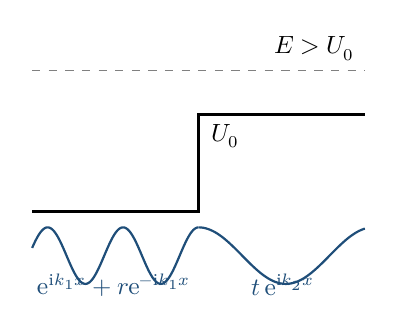
\begin{tikzpicture}
\begin{axis}[width=0.49\linewidth, height=4.8cm, axis lines=none, xmin=-6.5, xmax=6.5, ymin=-1.6, ymax=3.6, samples=300, clip=false]
  \addplot[very thick] coordinates {(-6.3,0) (0,0) (0,2.0) (6.3,2.0)};
  \addplot[gray, dashed] coordinates {(-6.3,2.9) (6.3,2.9)};
  \node[font=\small, anchor=south east] at (axis cs:6.3,2.9) {$E>U_0$};
  \node[font=\small, anchor=north west] at (axis cs:0.1,2.0) {$U_0$};
  \addplot[accent, thick, domain=-6.3:0] {-0.9+0.45*cos(deg(2.2*x))+0.13*cos(deg(-2.2*x))};
  \addplot[accent, thick, domain=0:6.3] {-0.9+0.58*cos(deg(0.95*x))};
  \node[font=\small, accent] at (axis cs:-3.2,-1.5) {$\ee^{\ii k_1x}+r\ee^{-\ii k_1x}$};
  \node[font=\small, accent] at (axis cs:3.2,-1.5) {$t\,\ee^{\ii k_2x}$};
  \node[font=\small] at (axis cs:0,-0.15) {};
\end{axis}
\end{tikzpicture}\hfill
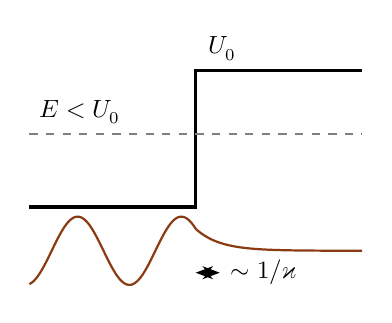
\begin{tikzpicture}
\begin{axis}[width=0.49\linewidth, height=4.8cm, axis lines=none, xmin=-6.5, xmax=6.5, ymin=-1.6, ymax=3.6, samples=300, clip=false]
  \addplot[very thick] coordinates {(-6.3,0) (0,0) (0,2.8) (6.3,2.8)};
  \addplot[gray, dashed] coordinates {(-6.3,1.5) (6.3,1.5)};
  \node[font=\small, anchor=south west] at (axis cs:-6.3,1.5) {$E<U_0$};
  \node[font=\small, anchor=south west] at (axis cs:0.1,2.8) {$U_0$};
  \addplot[keycol, thick, domain=-6.3:0] {-0.9+0.7*cos(deg(1.6*x)+50)};
  \addplot[keycol, thick, domain=0:6.3] {-0.9+0.7*cos(50)*exp(-1.1*x)};
  \draw[<->] (axis cs:0,-1.35) -- (axis cs:0.91,-1.35);
  \node[font=\small, anchor=west] at (axis cs:0.95,-1.35) {$\sim1/\varkappa$};
\end{axis}
\end{tikzpicture}
\caption{Потенциальная ступенька. Слева: $E>U_0$ — частичное отражение, прошедшая волна
имеет бо́льшую длину волны. Справа: $E<U_0$ — полное отражение (стоячая волна) и затухающая
волна под ступенькой. Показан ход $\operatorname{Re}\psi$ (качественно).}
\label{fig:7:step}
\end{figure}

\begin{figure}[htbp]
\centering
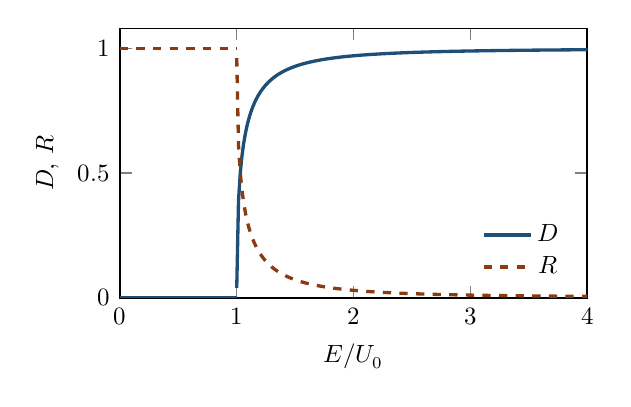
\begin{tikzpicture}
\begin{axis}[width=0.62\linewidth, height=5.0cm, xlabel={$E/U_0$}, ylabel={$D$, $R$},
   xmin=0, xmax=4, ymin=0, ymax=1.08, samples=200, legend pos=south east, legend style={font=\small, draw=none}]
  \addplot[accent, very thick, domain=1.0001:4] {4*sqrt(1-1/x)/(1+sqrt(1-1/x))^2};
  \addlegendentry{$D$}
  \addplot[keycol, very thick, dashed, domain=1.0001:4] {((1-sqrt(1-1/x))/(1+sqrt(1-1/x)))^2};
  \addlegendentry{$R$}
  \addplot[keycol, very thick, dashed, forget plot] coordinates {(0,1) (1,1)};
  \addplot[accent, very thick, forget plot] coordinates {(0,0) (1,0)};
\end{axis}
\end{tikzpicture}
\caption{Коэффициенты прохождения и отражения для ступеньки в зависимости от $E/U_0$
(расчёт по~\eqref{eq:7:stepRD}). При $E<U_0$ отражение полное.}
\label{fig:7:stepD}
\end{figure}

\subsection{Прямоугольный барьер}

Пусть $U(x)=U_0$ при $0<x<a$ и $U=0$ вне этого отрезка; $E<U_0$. В трёх областях:
\[
  \psi_{\mathrm I}=A\ee^{\ii kx}+B\ee^{-\ii kx},\quad
  \psi_{\mathrm{II}}=C\ee^{\varkappa x}+D'\ee^{-\varkappa x},\quad
  \psi_{\mathrm{III}}=F\ee^{\ii kx},
\]
$k=\sqrt{2mE}/\hbar$, $\varkappa=\sqrt{2m(U_0-E)}/\hbar$. Четыре условия сшивания при $x=0$ и $x=a$
дают (вывод~\ref{der:7:barrier}) точный коэффициент прохождения
\begin{equation}\label{eq:7:Dexact}
  D=\frac{|F|^2}{|A|^2}=\left[1+\frac{U_0^2\,\sh^2(\varkappa a)}{4E(U_0-E)}\right]^{-1}.
\end{equation}
$D>0$ при любых $a$ и $E$ — частица с конечной вероятностью проходит сквозь классически
непреодолимый барьер. Это \emph{туннельный эффект}. При $\varkappa a\gg1$ ($\sh\varkappa a\approx\frac12\ee^{\varkappa a}$):
\begin{equation}\label{eq:7:Dthick}
  D\approx\frac{16E(U_0-E)}{U_0^2}\,\ee^{-2\varkappa a}=D_0\exp\Bigl[-\frac2\hbar\sqrt{2m(U_0-E)}\,a\Bigr],
\end{equation}
где предэкспоненциальный множитель $D_0=16\frac{E}{U_0}\bigl(1-\frac{E}{U_0}\bigr)\le4$ — порядка единицы.
Определяющей является экспонента: $D$ экспоненциально мал и чрезвычайно чувствителен к ширине
барьера, его высоте и массе частицы.

\paragraph{Надбарьерное прохождение ($E>U_0$).} Замена $\varkappa\to\ii k'$, $k'=\sqrt{2m(E-U_0)}/\hbar$,
$\sh(\varkappa a)\to\ii\sin(k'a)$, $U_0-E\to-(E-U_0)$ даёт
\begin{equation}\label{eq:7:Dabove}
  D=\left[1+\frac{U_0^2\sin^2(k'a)}{4E(E-U_0)}\right]^{-1}.
\end{equation}
Даже над барьером $D<1$; но при $k'a=\pi n$ (на ширине барьера укладывается целое число
полуволн) $D=1$ — \emph{резонансное прохождение}: волны, отражённые от двух границ, гасят
друг друга. Аналог — просветление оптики. Для потенциальной ямы ($U_0<0$) этот эффект
объясняет аномально малое рассеяние медленных электронов на атомах благородных газов
(эффект Рамзауэра--Таунсенда).

\paragraph{Численные примеры.} Электрон, $E=1$~эВ, $U_0=2$~эВ:
$\varkappa=\sqrt{2\mel c^2(U_0-E)}/\hbar c=\sqrt{2\cdot0{,}511\cdot10^6\cdot1}/1973\ \text{Å}^{-1}=0{,}51\ \text{Å}^{-1}$.
При $a=5$~Å: $\varkappa a=2{,}6$, $D\approx16\cdot0{,}25\cdot\ee^{-5{,}1}\approx0{,}024$. Протон с теми же $E$, $U_0$, $a$:
$\varkappa$ больше в $\sqrt{1836}\approx43$ раза, $2\varkappa a\approx220$, $D\sim\ee^{-220}\sim10^{-96}$ —
практически нуль. Туннелирование — явление для лёгких частиц и тонких барьеров (или для очень
большого числа попыток, как в альфа-распаде).

\begin{figure}[htbp]
\centering
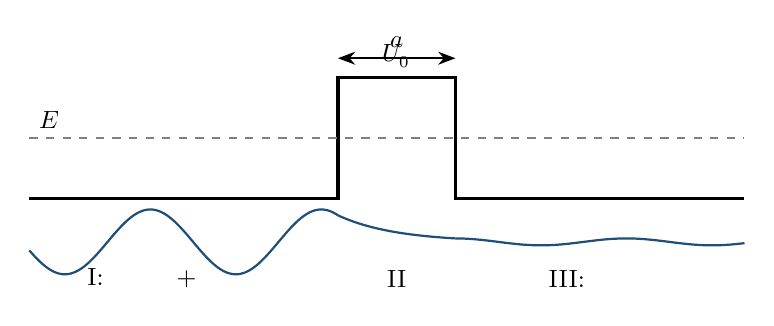
\begin{tikzpicture}
\begin{axis}[width=0.9\linewidth, height=4.6cm, axis lines=none, xmin=-6.5, xmax=8.5, ymin=-1.9, ymax=3.6, samples=300, clip=false]
  \addplot[very thick] coordinates {(-6.3,0) (0,0) (0,2.8) (2.4,2.8) (2.4,0) (8.3,0)};
  \addplot[gray, dashed] coordinates {(-6.3,1.4) (8.3,1.4)};
  \node[font=\small, anchor=south west] at (axis cs:-6.3,1.4) {$E$};
  \node[font=\small, anchor=south] at (axis cs:1.2,2.8) {$U_0$};
  \draw[<->] (axis cs:0,3.25) -- (axis cs:2.4,3.25) node[midway, above, font=\small] {$a$};
  \addplot[accent, thick, domain=-6.3:0] {-1.0+0.75*cos(deg(1.8*x)+35)};
  \addplot[accent, thick, domain=0:2.4] {-1.0+0.75*cos(35)*exp(-0.85*x)};
  \addplot[accent, thick, domain=2.4:8.3] {-1.0+0.75*cos(35)*exp(-0.85*2.4)*cos(deg(1.8*(x-2.4)))};
  \node[font=\small] at (axis cs:-3.2,-1.85) {I: падающая + отражённая};
  \node[font=\small] at (axis cs:1.2,-1.85) {II};
  \node[font=\small] at (axis cs:5.4,-1.85) {III: прошедшая};
\end{axis}
\end{tikzpicture}
\caption{Туннелирование через прямоугольный барьер ($E<U_0$): под барьером волновая функция
экспоненциально спадает, за барьером — бегущая волна малой амплитуды (качественно).}
\label{fig:7:barrier}
\end{figure}

\subsection{Барьер произвольной формы}

Для плавного барьера $U(x)$ и энергии $E$ ниже его вершины (рис.~\ref{fig:7:wkb}) в
квазиклассическом приближении (вывод~\ref{der:7:wkb})
\begin{equation}\label{eq:7:wkb}
  D\approx\exp\left[-\frac{2}{\hbar}\int_{x_1}^{x_2}\sqrt{2m\bigl(U(x)-E\bigr)}\,\dd x\right],
\end{equation}
где $x_1$, $x_2$ — точки поворота ($U(x_{1,2})=E$). \emph{Условия применимости:} показатель
экспоненты велик ($D\ll1$), и потенциал меняется плавно — мало меняется на длине
$1/\varkappa(x)$ (квазиклассичность: $|\dd\lambda/\dd x|\ll1$), кроме окрестностей точек поворота.
Предэкспоненциальный множитель порядка единицы при этом опускается.

\begin{figure}[htbp]
\centering
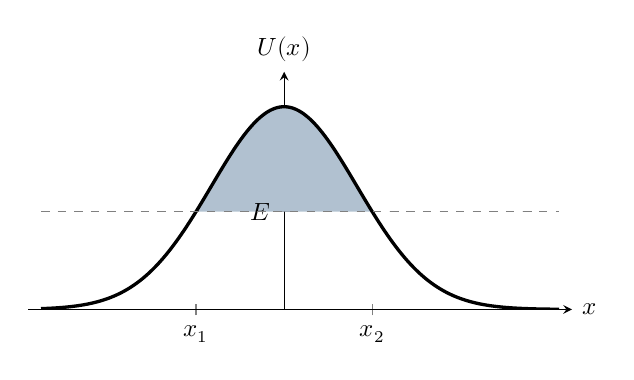
\begin{tikzpicture}
\begin{axis}[width=0.7\linewidth, height=4.6cm, axis lines=middle, xlabel={$x$}, ylabel={$U(x)$},
   xmin=-4, xmax=4.5, ymin=0, ymax=3.4, xtick={-1.38,1.38}, xticklabels={$x_1$,$x_2$}, ytick={1.4},
   yticklabels={$E$}, samples=200,
   xlabel style={at={(ticklabel* cs:1)}, anchor=west}, ylabel style={at={(ticklabel* cs:1)}, anchor=south}]
  \addplot[very thick, domain=-3.8:4.3, name path=U] {2.9*exp(-x^2/2.6)};
  \addplot[gray, dashed, domain=-3.8:4.3, name path=E] {1.4};
  \addplot[accent!35] fill between[of=U and E, soft clip={domain=-1.38:1.38}];
\end{axis}
\end{tikzpicture}
\caption{Барьер произвольной формы. Закрашена область $x_1<x<x_2$, где $U>E$; именно
интеграл по ней входит в показатель~\eqref{eq:7:wkb}.}
\label{fig:7:wkb}
\end{figure}

\paragraph{Пример 1: холодная (автоэлектронная) эмиссия.} В сильном поле $\mathcal E$ у
поверхности металла потенциальная энергия электрона вне металла $U(x)=E+A-e\mathcal Ex$ ($A$ —
работа выхода, $E$ — энергия электрона на уровне Ферми). Барьер треугольный, точки поворота
$x_1=0$, $x_2=A/e\mathcal E$:
\[
  \int_0^{A/e\mathcal E}\sqrt{2m(A-e\mathcal Ex)}\,\dd x=\sqrt{2m}\,\frac{2}{3}\frac{A^{3/2}}{e\mathcal E}
  \quad\Longrightarrow\quad
  D\approx\exp\Bigl(-\frac{4\sqrt{2m}\,A^{3/2}}{3\hbar e\mathcal E}\Bigr).
\]
Ток $\propto D$ резко растёт с полем (закон Фаулера--Нордгейма); заметная эмиссия начинается при
$\mathcal E\sim10^7$--$10^8$~В/см. На туннелировании основаны также сканирующий туннельный
микроскоп (ток экспоненциально зависит от зазора: изменение зазора на 1~Å меняет ток примерно на
порядок) и туннельный диод.

\paragraph{Пример 2: альфа-распад.} Альфа-частица в ядре туннелирует сквозь кулоновский барьер;
вычисление интеграла~\eqref{eq:7:wkb} приводит к формуле Гамова и закону Гейгера--Нэттола (\tref{t:19}).

\section{Математические выводы}

\begin{derivation}[label=der:7:step]{ступенька при $E>U_0$}
\emph{Решения.} При $x<0$: $\psi_1=\ee^{\ii k_1x}+r\ee^{-\ii k_1x}$ (амплитуда падающей волны
принята равной 1). При $x>0$: $\psi_2=t\ee^{\ii k_2x}$ (волны, идущей из $+\infty$, нет).

\emph{Сшивание при $x=0$:}
\[
  \psi_1(0)=\psi_2(0):\ 1+r=t;\qquad \psi_1'(0)=\psi_2'(0):\ \ii k_1(1-r)=\ii k_2t .
\]
Подставляя $t=1+r$ во второе: $k_1-k_1r=k_2+k_2r$, откуда
\[
  r=\frac{k_1-k_2}{k_1+k_2},\qquad t=1+r=\frac{2k_1}{k_1+k_2}.
\]
\emph{Потоки.} Для волны $c\,\ee^{\ii kx}$ поток $j=\hbar k|c|^2/m$. Поэтому
\[
  R=\frac{\hbar k_1|r|^2/m}{\hbar k_1/m}=\Bigl(\frac{k_1-k_2}{k_1+k_2}\Bigr)^2,\qquad
  D=\frac{\hbar k_2|t|^2/m}{\hbar k_1/m}=\frac{k_2}{k_1}\frac{4k_1^2}{(k_1+k_2)^2}=\frac{4k_1k_2}{(k_1+k_2)^2}.
\]
\emph{Проверка:} $R+D=\dfrac{k_1^2-2k_1k_2+k_2^2+4k_1k_2}{(k_1+k_2)^2}=1$. Важно: $D\neq|t|^2$, так как
скорости частиц по разные стороны ступеньки различны; коэффициенты определяются через потоки.
\end{derivation}

\begin{derivation}[label=der:7:stepbelow]{ступенька при $E<U_0$}
При $x>0$: $\psi_2=t\ee^{-\varkappa x}$ (растущее решение $\ee^{+\varkappa x}$ отброшено как неограниченное).
Сшивание: $1+r=t$, $\ii k(1-r)=-\varkappa t$. Отсюда $\ii k-\ii kr=-\varkappa-\varkappa r$ и
\[
  r=\frac{\ii k+\varkappa}{\ii k-\varkappa}=\frac{k-\ii\varkappa}{k+\ii\varkappa},\qquad
  |r|^2=\frac{k^2+\varkappa^2}{k^2+\varkappa^2}=1 .
\]
Таким образом $R=1$. Отражённая волна сдвинута по фазе: $r=\ee^{-2\ii\phi}$, $\tg\phi=\varkappa/k$.
Ток при $x>0$: $j=\frac{\hbar}{m}\operatorname{Im}(\psi_2^*\psi_2')=\frac{\hbar}{m}\operatorname{Im}(-\varkappa|t|^2\ee^{-2\varkappa x})=0$.
\end{derivation}

\begin{derivation}[label=der:7:barrier]{коэффициент прохождения прямоугольного барьера}
\emph{Шаг 1 (сшивание при $x=a$).}
\[
  C\ee^{\varkappa a}+D'\ee^{-\varkappa a}=F\ee^{\ii ka},\qquad
  \varkappa\bigl(C\ee^{\varkappa a}-D'\ee^{-\varkappa a}\bigr)=\ii kF\ee^{\ii ka}.
\]
Складывая и вычитая (после деления второго на $\varkappa$):
\[
  C=\frac{F\ee^{\ii ka}}{2}\Bigl(1+\frac{\ii k}{\varkappa}\Bigr)\ee^{-\varkappa a},\qquad
  D'=\frac{F\ee^{\ii ka}}{2}\Bigl(1-\frac{\ii k}{\varkappa}\Bigr)\ee^{\varkappa a}.
\]
\emph{Шаг 2 (сшивание при $x=0$).} $A+B=C+D'$, $\ii k(A-B)=\varkappa(C-D')$. Исключая $B$:
\[
  2A=(C+D')+\frac{\varkappa}{\ii k}(C-D')=C\Bigl(1-\frac{\ii\varkappa}{k}\Bigr)+D'\Bigl(1+\frac{\ii\varkappa}{k}\Bigr).
\]
\emph{Шаг 3 (подстановка).} Вычислим произведения:
\[
  \Bigl(1+\frac{\ii k}{\varkappa}\Bigr)\Bigl(1-\frac{\ii\varkappa}{k}\Bigr)=2+\ii\Bigl(\frac k\varkappa-\frac\varkappa k\Bigr),\qquad
  \Bigl(1-\frac{\ii k}{\varkappa}\Bigr)\Bigl(1+\frac{\ii\varkappa}{k}\Bigr)=2-\ii\Bigl(\frac k\varkappa-\frac\varkappa k\Bigr).
\]
Тогда
\begin{align*}
  2A&=\frac{F\ee^{\ii ka}}{2}\Bigl[2\bigl(\ee^{\varkappa a}+\ee^{-\varkappa a}\bigr)
     -\ii\Bigl(\frac k\varkappa-\frac\varkappa k\Bigr)\bigl(\ee^{\varkappa a}-\ee^{-\varkappa a}\bigr)\Bigr],\\
  A&=F\ee^{\ii ka}\Bigl[\ch\varkappa a+\ii\,\frac{\varkappa^2-k^2}{2k\varkappa}\,\sh\varkappa a\Bigr].
\end{align*}
\emph{Шаг 4 (коэффициент прохождения).} Скорости слева и справа одинаковы, поэтому $D=|F/A|^2$:
\[
  D^{-1}=\ch^2\varkappa a+\Bigl(\frac{\varkappa^2-k^2}{2k\varkappa}\Bigr)^2\sh^2\varkappa a
  =1+\Bigl[1+\frac{(\varkappa^2-k^2)^2}{4k^2\varkappa^2}\Bigr]\sh^2\varkappa a
  =1+\frac{(k^2+\varkappa^2)^2}{4k^2\varkappa^2}\sh^2\varkappa a ,
\]
где использовано $\ch^2=1+\sh^2$ и $4k^2\varkappa^2+(\varkappa^2-k^2)^2=(k^2+\varkappa^2)^2$.
\emph{Шаг 5.} Так как $k^2+\varkappa^2=2mU_0/\hbar^2$, $k^2\varkappa^2=(2m/\hbar^2)^2E(U_0-E)$:
\[
  \frac{(k^2+\varkappa^2)^2}{4k^2\varkappa^2}=\frac{U_0^2}{4E(U_0-E)}
  \quad\Longrightarrow\quad
  D=\Bigl[1+\frac{U_0^2\sh^2\varkappa a}{4E(U_0-E)}\Bigr]^{-1}.
\]
\emph{Предел $\varkappa a\gg1$:} $\sh^2\varkappa a\approx\frac14\ee^{2\varkappa a}\gg1$, единицей можно пренебречь:
$D\approx\dfrac{16E(U_0-E)}{U_0^2}\ee^{-2\varkappa a}$. \emph{Предел $a\to0$:} $D\to1$.
\end{derivation}

\begin{derivation}[label=der:7:wkb]{барьер произвольной формы (приближённый вывод)}
\emph{Допущения:} $D\ll1$; $U(x)$ меняется плавно; отражения на внутренних границах и
предэкспоненциальные множители не учитываются (их вклад — множитель порядка единицы).

Разобьём область $x_1<x<x_2$ на узкие прямоугольные барьеры шириной $\dd x_i$ с высотой
$U(x_i)$. Для каждого по~\eqref{eq:7:Dthick} $D_i\approx\exp[-2\varkappa(x_i)\,\dd x_i]$,
$\varkappa(x)=\sqrt{2m(U(x)-E)}/\hbar$. Прохождение через последовательность барьеров — последовательные
независимые события (при сделанных допущениях), поэтому
\[
  D\approx\prod_iD_i=\exp\Bigl[-2\sum_i\varkappa(x_i)\dd x_i\Bigr]\xrightarrow[\dd x_i\to0]{}
  \exp\Bigl[-\frac2\hbar\int_{x_1}^{x_2}\sqrt{2m(U(x)-E)}\,\dd x\Bigr].
\]
Строгий вывод использует квазиклассическое (ВКБ) решение уравнения Шредингера
$\psi\approx\frac{C}{\sqrt{\varkappa(x)}}\exp\bigl(\pm\int\varkappa\,\dd x\bigr)$ под барьером и сшивание вблизи
точек поворота; он подтверждает показатель экспоненты. Для прямоугольного барьера формула
воспроизводит~\eqref{eq:7:Dthick} с точностью до множителя $D_0$.
\end{derivation}

\section{Итоговые формулы}

\keyformula{R=\Bigl(\frac{k_1-k_2}{k_1+k_2}\Bigr)^2,\quad D=\frac{4k_1k_2}{(k_1+k_2)^2}\ (E>U_0);\qquad R=1\ (E<U_0)}
 {$k_1=\sqrt{2mE}/\hbar$, $k_2=\sqrt{2m(E-U_0)}/\hbar$.}
 {одномерная ступенька высоты $U_0$, стационарный поток частиц.}
 {вероятности отражения и прохождения; надбарьерное отражение.}

\keyformula{D=\Bigl[1+\frac{U_0^2\sh^2\varkappa a}{4E(U_0-E)}\Bigr]^{-1}\approx\frac{16E(U_0-E)}{U_0^2}\ee^{-2\varkappa a}}
 {$\varkappa=\sqrt{2m(U_0-E)}/\hbar$, $a$ — ширина, $U_0$ — высота барьера.}
 {прямоугольный барьер, $E<U_0$; приближение — при $\varkappa a\gg1$.}
 {вероятность туннелирования.}

\keyformula{D\approx\exp\Bigl[-\frac2\hbar\int_{x_1}^{x_2}\sqrt{2m(U(x)-E)}\,\dd x\Bigr]}
 {$x_1,x_2$ — точки поворота, $U(x_{1,2})=E$.}
 {квазиклассика: показатель $\gg1$, потенциал плавный; точность — до множителя порядка 1.}
 {туннелирование через барьер любой формы (эмиссия, альфа-распад, реакции синтеза).}

\keyformula{\delta=\frac{1}{2\varkappa}=\frac{\hbar}{2\sqrt{2m(U_0-E)}}}
 {$\delta$ — глубина проникновения под ступеньку (по плотности вероятности).}
 {$E<U_0$.}
 {масштаб области, куда частица «заходит» в классически запрещённую зону.}

\section{Физическая интерпретация}

\textbf{Зависимости.} Показатель туннельной экспоненты $\propto a\sqrt{m(U_0-E)}$: увеличение массы в
4 раза или ширины вдвое возводит $D$ в квадрат. Поэтому туннелирование электронов —
повседневное явление (контакты, СТМ, флеш-память), протонов — заметно в химии и термоядерном
синтезе в звёздах, а макротела не туннелируют.

\textbf{Предельные случаи.} $E\to U_0$: для ступеньки $R\to1$; $E\gg U_0$: $R\to0$, классический предел.
$\hbar\to0$: $D\to0$ при $E<U_0$ и $D\to1$ при $E>U_0$ — классическое поведение.

\textbf{Время и энергия.} Под барьером «кинетическая энергия отрицательна», но это не парадокс:
кинетическая энергия и координата не измеримы одновременно точно. Обнаружить частицу под барьером
на глубине $\delta$ можно, лишь сообщив ей энергию $\sim\hbar^2/m\delta^2\gtrsim U_0-E$.

\textbf{Эксперимент.} Туннельный эффект подтверждается холодной эмиссией, работой туннельного
диода (Эсаки, 1957), эффектом Джозефсона, СТМ (Бинниг и Рорер, 1981), законом Гейгера--Нэттола.

\section{Что необходимо знать на экзамене}

\begin{examcheck}
\checkhead{Определения}
\begin{itemize}
 \item задача рассеяния; коэффициенты $R$, $D$ через потоки; туннельный эффект.
\end{itemize}
\checkhead{Формулы}
\begin{itemize}
 \item ступенька: $R=((k_1-k_2)/(k_1+k_2))^2$, $D=4k_1k_2/(k_1+k_2)^2$; при $E<U_0$ $R=1$, $\delta=1/2\varkappa$;
 \item барьер: точная формула для $D$ и её предел $D\approx D_0\ee^{-2\varkappa a}$; резонанс при $k'a=\pi n$;
 \item квазиклассическая формула $D\approx\exp(-\frac2\hbar\int\sqrt{2m(U-E)}\dd x)$.
\end{itemize}
\checkhead{Выводы}
\begin{itemize}
 \item сшивание для ступеньки (оба случая), проверка $R+D=1$;
 \item коэффициент прохождения прямоугольного барьера (шаги 1--5);
 \item квазиклассическая формула как произведение коэффициентов тонких барьеров; треугольный барьер.
\end{itemize}
\checkhead{Интерпретации}
\begin{itemize}
 \item почему $D\neq|t|^2$; надбарьерное отражение; оптические аналогии;
 \item экспоненциальная чувствительность к массе и ширине (электрон vs протон); применения.
\end{itemize}
\end{examcheck}

% ======================================================================
\chapter[Гармонический осциллятор]%
        {Одномерный гармонический осциллятор}
\label{t:08}
% ======================================================================

\begin{qbox}
\textbf{Билет 8.} Уровни энергии одномерного гармонического осциллятора (без вывода).
Волновая функция основного состояния одномерного осциллятора.
\end{qbox}

\section{Содержание билета}

\textbf{Подтемы:}
\begin{enumerate}
 \item постановка задачи: гамильтониан и стационарное уравнение Шредингера для осциллятора;
 \item спектр $E_n=\hbar\omega(n+\frac12)$ — формулировка и обсуждение \emph{(без вывода, по программе)};
 \item волновая функция основного состояния: получение, нормировка, проверка подстановкой;
 \item энергия нулевых колебаний, её оценка из соотношения неопределённостей и экспериментальные проявления;
 \item возбуждённые состояния (качественно), правила отбора, применения.
\end{enumerate}

\textbf{Необходимые понятия:} стационарное уравнение Шредингера (\tref{t:06});
соотношение неопределённостей (\tref{t:02}, \tref{t:05}); гауссовы интегралы; классический
осциллятор $x=x_0\cos\omega t$.

\section{Определения и физические принципы}

\begin{definition}[гармонический осциллятор]
Частица массы $m$ в потенциале $U(x)=\dfrac{m\omega^2x^2}{2}=\dfrac{kx^2}{2}$, где $\omega=\sqrt{k/m}$ —
классическая частота колебаний. Гамильтониан
\begin{equation}\label{eq:8:H}
  \op H=\frac{\op p^2}{2m}+\frac{m\omega^2x^2}{2}=-\frac{\hbar^2}{2m}\diff{^2}{x^2}+\frac{m\omega^2x^2}{2}.
\end{equation}
\end{definition}

\emph{Почему осциллятор важен.} Любой гладкий потенциал вблизи минимума $x_0$ приближённо
квадратичен: $U(x)\approx U(x_0)+\frac12U''(x_0)(x-x_0)^2$. Поэтому малые колебания атомов в
молекулах и кристаллах, колебания мод электромагнитного поля (фотоны), фононы — всё это
осцилляторы. \emph{Область применимости модели:} амплитуда колебаний мала по сравнению с масштабом,
на котором потенциал отклоняется от параболы (ангармонизм).

\begin{definition}[естественные масштабы]
Параметры $m,\omega,\hbar$ задают единственные масштабы длины и энергии:
\begin{equation}\label{eq:8:scales}
  x_0=\sqrt{\frac{\hbar}{m\omega}},\qquad \hbar\omega,\qquad \xi=\frac{x}{x_0}.
\end{equation}
$x_0$ — амплитуда классических колебаний с энергией $\hbar\omega/2$.
\end{definition}

\section{Основная теория}

\subsection{Уравнение и спектр}

Стационарное уравнение Шредингера
\begin{equation}\label{eq:8:sse}
  -\frac{\hbar^2}{2m}\psi''+\frac{m\omega^2x^2}{2}\psi=E\psi
\end{equation}
в безразмерных переменных $\xi=x/x_0$, $\varepsilon=2E/\hbar\omega$ принимает вид
\begin{equation}\label{eq:8:dimless}
  \diff{^2\psi}{\xi^2}+(\varepsilon-\xi^2)\psi=0 .
\end{equation}
Потенциал неограниченно растёт, движение финитно при любой энергии — спектр целиком дискретный.

\begin{principle}{Уровни энергии осциллятора (без вывода)}
Решения~\eqref{eq:8:dimless}, удовлетворяющие условию $\psi\to0$ при $|\xi|\to\infty$, существуют
только при $\varepsilon=2n+1$, т.\,е.
\begin{equation}\label{eq:8:En}
  E_n=\hbar\omega\Bigl(n+\frac12\Bigr),\qquad n=0,1,2,\dots
\end{equation}
Соответствующие волновые функции
$\psi_n(\xi)=\dfrac{1}{\sqrt{2^nn!\sqrt\pi\,x_0}}\,H_n(\xi)\,\ee^{-\xi^2/2}$,
где $H_n$ — полиномы Эрмита: $H_0=1$, $H_1=2\xi$, $H_2=4\xi^2-2$, $H_3=8\xi^3-12\xi$.
\end{principle}

\emph{Комментарий к «выводу».} Вывод основан на том, что при больших $|\xi|$ решение ведёт себя как
$\ee^{\pm\xi^2/2}$; подстановка $\psi=h(\xi)\ee^{-\xi^2/2}$ даёт уравнение для $h$, решение которого
в виде степенного ряда растёт как $\ee^{\xi^2}$, если ряд не обрывается. Обрыв ряда на $n$-м члене
и даёт условие $\varepsilon=2n+1$. Альтернативный вывод — алгебраический метод
операторов рождения и уничтожения. По программе вывод не требуется.

\paragraph{Свойства спектра.}
\begin{enumerate}
 \item \textbf{Эквидистантность:} $E_{n+1}-E_n=\hbar\omega$ для всех $n$. Это совпадает с гипотезой
       Планка об обмене энергией порциями $\hbar\omega$, но в квантовой механике она \emph{следует} из
       уравнения Шредингера.
 \item \textbf{Энергия нулевых колебаний} $E_0=\hbar\omega/2>0$: осциллятор не может покоиться в минимуме
       потенциала (вывод~\ref{der:8:uncert}).
 \item \textbf{Невырожденность:} каждому уровню отвечает одна функция (общее свойство связанных
       состояний одномерного движения).
 \item \textbf{Чётность:} $\psi_n(-x)=(-1)^n\psi_n(x)$ — следствие чётности $U(x)$.
 \item \textbf{Узлы:} $\psi_n$ имеет $n$ нулей.
 \item \textbf{Правило отбора} для дипольных переходов: $\Delta n=\pm1$ (матричный элемент
       $\int\psi_{n'}x\psi_n\dd x\neq0$ лишь при $n'=n\pm1$). Поэтому излучение осциллятора имеет
       единственную частоту $\omega$, как и в классике.
\end{enumerate}

\subsection{Основное состояние}

Основное состояние ($n=0$) — гауссова функция (вывод~\ref{der:8:ground}):
\begin{equation}\label{eq:8:psi0}
  \psi_0(x)=\Bigl(\frac{m\omega}{\pi\hbar}\Bigr)^{1/4}\exp\Bigl(-\frac{m\omega x^2}{2\hbar}\Bigr)
  =\frac{1}{\pi^{1/4}\sqrt{x_0}}\,\ee^{-x^2/2x_0^2},\qquad E_0=\frac{\hbar\omega}{2}.
\end{equation}
Свойства: $\avg x=0$, $\avg{x^2}=x_0^2/2$, $\avg{p^2}=\hbar^2/(2x_0^2)$ (вывод~\ref{der:8:means}),
\[
  \Delta x\,\Delta p=\frac{x_0}{\sqrt2}\cdot\frac{\hbar}{\sqrt2x_0}=\frac\hbar2,\qquad
  \avg T=\avg U=\frac{\hbar\omega}{4}.
\]
Основное состояние осциллятора — состояние с минимальной неопределённостью; средние кинетическая
и потенциальная энергии равны (теорема вириала для квадратичного потенциала).

\paragraph{Выход за классические точки поворота.} Классически частица с энергией $\hbar\omega/2$
колеблется между $\pm x_0$. Квантовая плотность $|\psi_0|^2$ отлична от нуля и при $|x|>x_0$.
Вероятность обнаружить частицу в классически запрещённой области
\[
  w=2\int_{x_0}^{\infty}|\psi_0|^2\dd x=\frac{2}{\sqrt\pi}\int_1^\infty\ee^{-\xi^2}\dd\xi=\operatorname{erfc}(1)\approx0{,}16 .
\]

\begin{figure}[htbp]
\centering
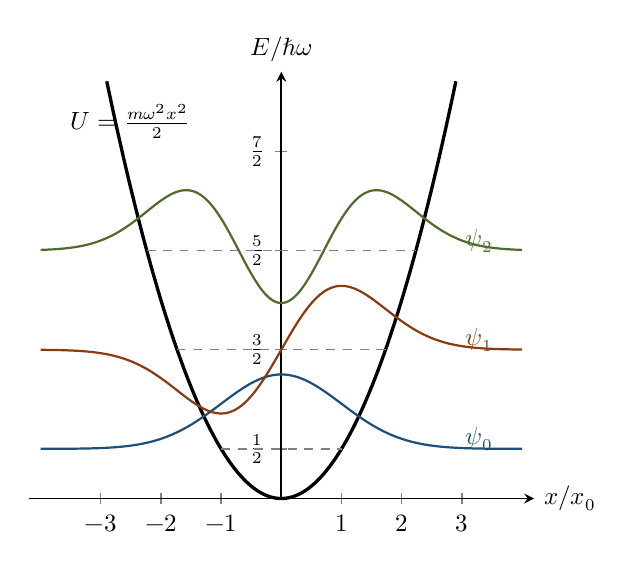
\begin{tikzpicture}
\begin{axis}[width=0.66\linewidth, height=7.0cm, axis lines=middle,
   xlabel={$x/x_0$}, ylabel={$E/\hbar\omega$}, xmin=-4.2, xmax=4.2, ymin=0, ymax=4.3,
   xtick={-3,-2,-1,1,2,3}, ytick={0.5,1.5,2.5,3.5},
   yticklabels={$\tfrac12$,$\tfrac32$,$\tfrac52$,$\tfrac72$},
   samples=200, clip=false,
   xlabel style={at={(ticklabel* cs:1)}, anchor=west},
   ylabel style={at={(ticklabel* cs:1)}, anchor=south}]
  \addplot[very thick, domain=-2.9:2.9] {x^2/2};
  \foreach \n in {0,1,2} {
    \pgfmathsetmacro{\En}{\n+0.5}
    \pgfmathsetmacro{\xt}{sqrt(2*\n+1)}
    \addplot[gray, dashed, domain=-\xt:\xt] {\En};
  }
  \addplot[accent, thick, domain=-4:4] {0.5 + 0.75*exp(-x^2/2)};
  \addplot[keycol, thick, domain=-4:4] {1.5 + 0.75*1.414*x*exp(-x^2/2)};
  \addplot[dercol, thick, domain=-4:4] {2.5 + 0.75*0.707*(2*x^2-1)*exp(-x^2/2)};
  \node[font=\small, accent, anchor=west] at (axis cs:2.9,0.6) {$\psi_0$};
  \node[font=\small, keycol, anchor=west] at (axis cs:2.9,1.6) {$\psi_1$};
  \node[font=\small, dercol, anchor=west] at (axis cs:2.9,2.6) {$\psi_2$};
  \node[font=\small] at (axis cs:-2.5,3.8) {$U=\frac{m\omega^2x^2}{2}$};
\end{axis}
\end{tikzpicture}
\caption{Потенциал осциллятора, эквидистантные уровни $E_n=\hbar\omega(n+\frac12)$ и волновые
функции трёх нижних состояний (смещены на уровень соответствующей энергии; масштаб по
вертикали для $\psi_n$ произвольный). Штриховые отрезки ограничены классическими точками
поворота $\pm\sqrt{2n+1}\,x_0$; волновые функции заходят за них.}
\label{fig:8:osc}
\end{figure}

\subsection{Энергия нулевых колебаний: проявления}

\begin{itemize}
 \item \textbf{Гелий} не затвердевает при нормальном давлении вплоть до $T\to0$: энергия нулевых
       колебаний лёгких атомов в «решётке» превышает выигрыш от слабого ван-дер-ваальсова притяжения.
 \item \textbf{Изотопический эффект в молекулах:} энергия диссоциации $D_0=D_e-\hbar\omega/2$ зависит
       от массы ядер через $\omega\propto1/\sqrt\mu$; у D$_2$ нулевая энергия меньше, и молекула связана
       сильнее, чем H$_2$.
 \item \textbf{Рассеяние рентгеновских лучей кристаллами} не исчезает полностью при $T\to0$: атомы
       колеблются около узлов и при абсолютном нуле (фактор Дебая--Уоллера остаётся меньше единицы).
 \item \textbf{Нулевые колебания электромагнитного поля} (энергия $\hbar\omega/2$ на моду) проявляются
       в эффекте Казимира и лэмбовском сдвиге.
\end{itemize}

\subsection{Применения}

Каждая мода электромагнитного поля в полости — осциллятор; состояние с $n$ квантами — $n$ фотонов
моды, $E=\hbar\omega(n+\frac12)$. Колебательные уровни двухатомной молекулы $E_v=\hbar\omega(v+\frac12)$
(\tref{t:11}); фононы в кристалле — кванты нормальных колебаний решётки.

\section{Математические выводы}

\begin{derivation}[label=der:8:uncert]{оценка энергии основного состояния из соотношения неопределённостей}
В основном состоянии из-за симметрии $\avg x=\avg p=0$, поэтому $\avg{x^2}=(\Delta x)^2$,
$\avg{p^2}=(\Delta p)^2$, и
\[
  E=\frac{(\Delta p)^2}{2m}+\frac{m\omega^2(\Delta x)^2}{2}\ge\frac{\hbar^2}{8m(\Delta x)^2}+\frac{m\omega^2(\Delta x)^2}{2},
\]
где использовано $\Delta p\ge\hbar/(2\Delta x)$. Минимизируем по $u=(\Delta x)^2$:
$\dfrac{\dd}{\dd u}\Bigl(\dfrac{\hbar^2}{8mu}+\dfrac{m\omega^2u}{2}\Bigr)=-\dfrac{\hbar^2}{8mu^2}+\dfrac{m\omega^2}{2}=0$
$\Rightarrow$ $u=\dfrac{\hbar}{2m\omega}$. Подставляя: $E_{\min}=\dfrac{\hbar\omega}{4}+\dfrac{\hbar\omega}{4}=\dfrac{\hbar\omega}{2}$.

Оценка совпадает с точным значением, потому что основное состояние осциллятора — гауссово,
для которого соотношение неопределённостей обращается в равенство. Физический смысл: сжатие волновой
функции уменьшает $\avg U$, но увеличивает $\avg T$; минимум суммы достигается при $\Delta x=x_0/\sqrt2$.
\end{derivation}

\begin{derivation}[label=der:8:ground]{волновая функция основного состояния}
\emph{Способ 1 (подбор вида решения).} Основное состояние не имеет узлов, чётно и должно убывать
на бесконечности быстрее любой степени. Попробуем $\psi_0=C\ee^{-\beta x^2}$, $\beta>0$. Вычислим
производные:
\[
  \psi_0'=-2\beta x\,\psi_0,\qquad \psi_0''=(-2\beta+4\beta^2x^2)\psi_0 .
\]
Подставим в~\eqref{eq:8:sse} и разделим на $\psi_0$:
\[
  -\frac{\hbar^2}{2m}\bigl(4\beta^2x^2-2\beta\bigr)+\frac{m\omega^2x^2}{2}=E .
\]
Равенство должно выполняться при всех $x$, поэтому коэффициент при $x^2$ равен нулю, а
свободные члены совпадают:
\[
  -\frac{2\hbar^2\beta^2}{m}+\frac{m\omega^2}{2}=0\ \Rightarrow\ \beta=\frac{m\omega}{2\hbar};\qquad
  E=\frac{\hbar^2\beta}{m}=\frac{\hbar\omega}{2}.
\]
(Корень $\beta=-m\omega/2\hbar$ отброшен — функция была бы ненормируемой.)

\emph{Способ 2 (факторизация).} Гамильтониан можно записать как
$\op H=\hbar\omega\bigl(\op a^\dagger\op a+\frac12\bigr)$, где
$\op a=\frac{1}{\sqrt2}\bigl(\xi+\diff{}{\xi}\bigr)$. Поскольку $\avg{\op a^\dagger\op a}=\int|\op a\psi|^2\ge0$,
энергия не меньше $\hbar\omega/2$, и минимум достигается при $\op a\psi_0=0$:
\[
  \xi\psi_0+\diff{\psi_0}{\xi}=0\quad\Longrightarrow\quad\frac{\dd\psi_0}{\psi_0}=-\xi\,\dd\xi
  \quad\Longrightarrow\quad\psi_0=C\ee^{-\xi^2/2}=C\ee^{-m\omega x^2/2\hbar}.
\]

\emph{Нормировка.} С интегралом Пуассона $\int_{-\infty}^\infty\ee^{-\alpha x^2}\dd x=\sqrt{\pi/\alpha}$ при
$\alpha=m\omega/\hbar$:
\[
  |C|^2\int_{-\infty}^{\infty}\ee^{-m\omega x^2/\hbar}\dd x=|C|^2\sqrt{\frac{\pi\hbar}{m\omega}}=1
  \quad\Longrightarrow\quad C=\Bigl(\frac{m\omega}{\pi\hbar}\Bigr)^{1/4}.
\]
\emph{Проверка размерности:} $[m\omega x^2/\hbar]=\text{г}\cdot\text{с}^{-1}\text{см}^2/(\text{эрг}\cdot\text{с})=1$;
$[C^2]=\text{см}^{-1}$, как и положено одномерной плотности вероятности.
\end{derivation}

\begin{derivation}[label=der:8:means]{средние значения в основном состоянии}
$|\psi_0|^2=\dfrac{1}{\sqrt\pi x_0}\ee^{-x^2/x_0^2}$ — нормальное распределение с дисперсией $\sigma^2=x_0^2/2$.
Поэтому $\avg x=0$, $\avg{x^2}=x_0^2/2=\hbar/(2m\omega)$, и
\[
  \avg U=\frac{m\omega^2}{2}\cdot\frac{\hbar}{2m\omega}=\frac{\hbar\omega}{4}.
\]
Кинетическая энергия: $\avg T=E_0-\avg U=\hbar\omega/4$; непосредственно —
$\avg{p^2}=\hbar^2\int|\psi_0'|^2\dd x=\hbar^2\int\frac{x^2}{x_0^4}|\psi_0|^2\dd x=\frac{\hbar^2}{x_0^4}\cdot\frac{x_0^2}{2}=\frac{\hbar^2}{2x_0^2}=\frac{m\hbar\omega}{2}$,
$\avg T=\avg{p^2}/2m=\hbar\omega/4$. Результаты согласуются.
\end{derivation}

\begin{derivation}[label=der:8:psi1]{проверка первого возбуждённого состояния}
Пусть $\psi_1=Cx\,\ee^{-\beta x^2}$, $\beta=m\omega/2\hbar$. Тогда
$\psi_1'=C(1-2\beta x^2)\ee^{-\beta x^2}$,
$\psi_1''=C(-6\beta x+4\beta^2x^3)\ee^{-\beta x^2}=(-6\beta+4\beta^2x^2)\psi_1$.
Подставляя в~\eqref{eq:8:sse}: $-\frac{\hbar^2}{2m}(4\beta^2x^2-6\beta)+\frac{m\omega^2x^2}{2}=E$. Члены с
$x^2$ сокращаются при том же $\beta$, а $E=3\hbar^2\beta/m=\frac32\hbar\omega$ — в согласии с~\eqref{eq:8:En}
при $n=1$. Функция нечётна и имеет один узел.
\end{derivation}

\section{Итоговые формулы}

\keyformula{E_n=\hbar\omega\Bigl(n+\frac12\Bigr),\qquad n=0,1,2,\dots}
 {$\omega=\sqrt{k/m}$ — классическая частота, $n$ — колебательное квантовое число.}
 {строго параболический потенциал (малые колебания); вывод не требуется.}
 {уровни энергии, частоты переходов ($\Delta n=\pm1$ $\Rightarrow$ $\omega$), нулевая энергия.}

\keyformula{\psi_0(x)=\Bigl(\frac{m\omega}{\pi\hbar}\Bigr)^{1/4}\exp\Bigl(-\frac{m\omega x^2}{2\hbar}\Bigr),\qquad E_0=\frac{\hbar\omega}{2}}
 {$x_0=\sqrt{\hbar/m\omega}$ — характерная длина; $|\psi_0|^2$ — гауссово распределение с $\sigma^2=x_0^2/2$.}
 {основное состояние.}
 {распределение координаты, средние энергии, вероятность выхода за точки поворота ($\approx16\,\%$).}

\keyformula{\Delta x=\frac{x_0}{\sqrt2},\quad \Delta p=\frac{\hbar}{\sqrt2x_0},\quad \Delta x\Delta p=\frac\hbar2,\quad \avg T=\avg U=\frac{\hbar\omega}{4}}
 {$x_0=\sqrt{\hbar/m\omega}$.}
 {основное состояние.}
 {основное состояние — состояние минимальной неопределённости.}

\section{Физическая интерпретация}

\textbf{Предельные случаи и соответствие.} При больших $n$ плотность $|\psi_n|^2$, усреднённая по
осцилляциям, приближается к классической плотности $w_{\text{кл}}(x)=1/(\pi\sqrt{A^2-x^2})$, которая
максимальна вблизи точек поворота (там частица движется медленно). Основное состояние, наоборот,
имеет максимум в центре — сугубо квантовое поведение.

\textbf{Зависимость от параметров.} $\hbar\omega=\hbar\sqrt{k/m}$: лёгкие частицы и жёсткие связи дают
большие кванты. Для молекулы H$_2$ $\hbar\omega\approx0{,}55$~эВ $\gg k_{\mathrm B}T_{\text{комн}}\approx0{,}026$~эВ —
колебания при комнатной температуре «заморожены» в основном состоянии; это объясняет
теплоёмкость двухатомных газов $C_V=\frac52R$ вместо $\frac72R$.

\textbf{Сравнение с ямой.} В бесконечной яме $E_n\propto n^2$ (уровни расходятся), в осцилляторе
$E_n\propto n$ (эквидистантны), в кулоновском поле $E_n\propto-1/n^2$ (сгущаются). Характер спектра
определяется тем, как быстро потенциал растёт с расстоянием.

\section{Что необходимо знать на экзамене}

\begin{examcheck}
\checkhead{Определения}
\begin{itemize}
 \item гамильтониан осциллятора; масштаб $x_0=\sqrt{\hbar/m\omega}$; энергия нулевых колебаний.
\end{itemize}
\checkhead{Формулы}
\begin{itemize}
 \item $E_n=\hbar\omega(n+\frac12)$ (без вывода); $\psi_0=(m\omega/\pi\hbar)^{1/4}\ee^{-m\omega x^2/2\hbar}$;
 \item $\avg{x^2}=\hbar/2m\omega$, $\avg T=\avg U=\hbar\omega/4$, $\Delta x\Delta p=\hbar/2$.
\end{itemize}
\checkhead{Выводы}
\begin{itemize}
 \item получение $\psi_0$ и $E_0$ подстановкой гауссовой функции; нормировка;
 \item оценка $E_0=\hbar\omega/2$ из соотношения неопределённостей;
 \item (желательно) проверка $\psi_1\propto x\ee^{-\beta x^2}$ и $E_1=\frac32\hbar\omega$.
\end{itemize}
\checkhead{Интерпретации}
\begin{itemize}
 \item эквидистантность и правило отбора $\Delta n=\pm1$; чётность и узлы $\psi_n$;
 \item проникновение за классические точки поворота; проявления нулевых колебаний (He, изотопы, Казимир).
\end{itemize}
\end{examcheck}

% ======================================================================
\chapter[Оператор момента импульса]%
        {Оператор момента импульса. Собственные значения \texorpdfstring{$L_z$ и $L^2$}{Lz и L²}}
\label{t:09}
% ======================================================================

\begin{qbox}
\textbf{Билет 9.} Оператор момента импульса. Собственные функции и собственные значения
оператора $L_z$ ($z$-компоненты момента импульса) в сферических координатах. Собственные значения
оператора квадрата момента импульса $L^2$ (без вывода).
\end{qbox}

\section{Содержание билета}

\textbf{Подтемы:}
\begin{enumerate}
 \item оператор момента импульса $\op{\vect L}=\vect r\times\op{\vect p}$, его компоненты в декартовых координатах;
 \item коммутационные соотношения и их следствие: одновременно измеримы лишь $L^2$ и одна проекция;
 \item $\op L_z=-\ii\hbar\,\partial/\partial\varphi$ в сферических координатах; собственные функции $\ee^{\ii m\varphi}$ и значения $m\hbar$;
 \item собственные значения $L^2=\hbar^2l(l+1)$ \emph{(без вывода)}; сферические функции; векторная модель.
\end{enumerate}

\textbf{Необходимые понятия:} операторы, коммутаторы, собственные функции (\tref{t:05});
сферические координаты $(r,\theta,\varphi)$; классический момент импульса.

\section{Определения и физические принципы}

\begin{definition}[оператор момента импульса]
По правилу соответствия $\vect L=\vect r\times\vect p\to\op{\vect L}=\vect r\times\op{\vect p}=-\ii\hbar\,\vect r\times\nabla$:
\begin{equation}\label{eq:9:L}
  \op L_x=-\ii\hbar\Bigl(y\pdiff{}{z}-z\pdiff{}{y}\Bigr),\quad
  \op L_y=-\ii\hbar\Bigl(z\pdiff{}{x}-x\pdiff{}{z}\Bigr),\quad
  \op L_z=-\ii\hbar\Bigl(x\pdiff{}{y}-y\pdiff{}{x}\Bigr),
\end{equation}
$\op L^2=\op L_x^2+\op L_y^2+\op L_z^2$. Порядок сомножителей несуществен: $y$ и $\op p_z$ коммутируют.
\end{definition}

\begin{definition}[квантовые числа момента]
$l=0,1,2,\dots$ — \emph{орбитальное} (азимутальное) квантовое число, определяющее $L^2=\hbar^2l(l+1)$;
$m=-l,\dots,l$ — \emph{магнитное} квантовое число, $L_z=m\hbar$. Состояния с $l=0,1,2,3,4$
обозначают буквами $s,p,d,f,g$.
\end{definition}

\emph{Физический смысл.} Момент импульса сохраняется в центрально-симметричном поле
($\op L^2$ и $\op L_z$ коммутируют с гамильтонианом); поэтому квантовые числа $l,m$ классифицируют
состояния атомов, ядер, молекул. Квантование момента — следствие однозначности волновой функции
при повороте на $2\pi$, а не постулат, как у Бора.

\emph{Область применимости.} Речь идёт об \emph{орбитальном} моменте частицы, связанном с её
движением в пространстве. Собственный момент (спин, \tref{t:12}) описывается теми же коммутационными
соотношениями, но может принимать и полуцелые значения; орбитальный — только целые.

\section{Основная теория}

\subsection{Коммутационные соотношения}

Из $[\op x,\op p_x]=\ii\hbar$ следует (вывод~\ref{der:9:comm})
\begin{equation}\label{eq:9:comm}
  [\op L_x,\op L_y]=\ii\hbar\op L_z,\qquad [\op L_y,\op L_z]=\ii\hbar\op L_x,\qquad [\op L_z,\op L_x]=\ii\hbar\op L_y,
\end{equation}
\begin{equation}\label{eq:9:L2comm}
  [\op L^2,\op L_x]=[\op L^2,\op L_y]=[\op L^2,\op L_z]=0 .
\end{equation}
\textbf{Следствия.} (1) Разные проекции момента не измеримы одновременно: если $L_z$ определена,
то $L_x$ и $L_y$ не имеют определённых значений (исключение — состояние $l=0$, где все проекции нули).
(2) Квадрат момента и одна (любая) проекция измеримы одновременно. Принято выбирать ось $z$;
состояние задаётся парой $(l,m)$. (3) Вектор $\vect L$ не может быть определён полностью — нельзя
сказать, «куда он направлен».

\subsection{Оператор $\op L_z$ в сферических координатах}

В сферических координатах $x=r\sin\theta\cos\varphi$, $y=r\sin\theta\sin\varphi$, $z=r\cos\theta$
(вывод~\ref{der:9:Lz}):
\begin{equation}\label{eq:9:Lzsph}
  \op L_z=-\ii\hbar\pdiff{}{\varphi}.
\end{equation}
$\op L_z$ действует только на азимутальный угол — это генератор поворотов вокруг оси $z$, подобно тому
как $\op p_x=-\ii\hbar\,\partial/\partial x$ — генератор сдвигов вдоль $x$.

\subsection{Собственные функции и значения $\op L_z$}

Уравнение $\op L_z\Phi=L_z\Phi$ решается элементарно (вывод~\ref{der:9:eig}):
\begin{equation}\label{eq:9:Phim}
  \Phi_m(\varphi)=\frac{1}{\sqrt{2\pi}}\ee^{\ii m\varphi},\qquad L_z=m\hbar,\qquad m=0,\pm1,\pm2,\dots
\end{equation}
Дискретность — следствие требования однозначности: точкам $\varphi$ и $\varphi+2\pi$ отвечает одна и та же
точка пространства. Функции ортонормированы на $[0,2\pi)$:
$\int_0^{2\pi}\Phi_{m'}^*\Phi_m\dd\varphi=\delta_{mm'}$. В состоянии $\Phi_m$ плотность вероятности
$|\Phi_m|^2=1/2\pi$ не зависит от $\varphi$ — азимутальный угол полностью неопределён (аналог
соотношения неопределённостей для пары $\varphi$, $L_z$).

\subsection{Квадрат момента (без вывода)}

В сферических координатах $\op L^2$ действует только на углы:
\begin{equation}\label{eq:9:L2}
  \op L^2=-\hbar^2\Bigl[\frac{1}{\sin\theta}\pdiff{}{\theta}\Bigl(\sin\theta\pdiff{}{\theta}\Bigr)
  +\frac{1}{\sin^2\theta}\pdiff{^2}{\varphi^2}\Bigr]\equiv-\hbar^2\Delta_{\theta,\varphi},
\end{equation}
где $\Delta_{\theta,\varphi}$ — угловая часть лапласиана: $\nabla^2=\frac{1}{r^2}\pdiff{}{r}\bigl(r^2\pdiff{}{r}\bigr)+\frac{1}{r^2}\Delta_{\theta,\varphi}$.

\begin{principle}{Собственные значения $\op L^2$ (без вывода)}
Однозначные и конечные на сфере решения уравнения $\op L^2Y=L^2Y$ существуют только при
\begin{equation}\label{eq:9:L2eig}
  L^2=\hbar^2l(l+1),\qquad l=0,1,2,\dots,
\end{equation}
причём при данном $l$ проекция $L_z=m\hbar$ может принимать $2l+1$ значений $m=-l,-l+1,\dots,l$.
Общие собственные функции $\op L^2$ и $\op L_z$ — \emph{сферические функции}
$Y_{lm}(\theta,\varphi)=\Theta_{lm}(\theta)\,\ee^{\ii m\varphi}$; уровень $L^2$ вырожден с кратностью $2l+1$.
\end{principle}

Примеры нормированных сферических функций ($\int|Y_{lm}|^2\sin\theta\,\dd\theta\,\dd\varphi=1$):
\[
  Y_{00}=\frac{1}{\sqrt{4\pi}},\qquad
  Y_{10}=\sqrt{\frac{3}{4\pi}}\cos\theta,\qquad
  Y_{1,\pm1}=\mp\sqrt{\frac{3}{8\pi}}\sin\theta\,\ee^{\pm\ii\varphi}.
\]
Проверка для $Y_{10}$ дана в выводе~\ref{der:9:Y10}.

\paragraph{Почему $|m|\le l$.} В состоянии с определёнными $l,m$
$\avg{L_x^2}+\avg{L_y^2}=\avg{L^2}-m^2\hbar^2=\hbar^2[l(l+1)-m^2]\ge0$, так как средние квадратов
эрмитовых операторов неотрицательны. Значит, $m^2\le l(l+1)$, т.\,е. $|m|\le l$. При $|m|=l$ всё равно
$\avg{L_x^2}+\avg{L_y^2}=\hbar^2l>0$: момент не может быть направлен точно вдоль оси $z$
(иначе все три проекции были бы определены).

\paragraph{Правдоподобность $l(l+1)$.} Для изотропного (неполяризованного) набора состояний
с данным $l$ все три оси равноправны, поэтому $\avg{L^2}=3\avg{L_z^2}$. Усредняя $m^2$ по $2l+1$
равновероятным значениям:
\[
  \avg{L_z^2}=\frac{\hbar^2}{2l+1}\sum_{m=-l}^{l}m^2=\frac{\hbar^2}{2l+1}\cdot\frac{l(l+1)(2l+1)}{3}=\frac{\hbar^2l(l+1)}{3},
\]
откуда $\avg{L^2}=\hbar^2l(l+1)$. Это не вывод~\eqref{eq:9:L2eig}, но наглядное объяснение,
почему $L^2$ больше $(l\hbar)^2$.

\subsection{Векторная модель}

Наглядно вектор $\vect L$ длины $\hbar\sqrt{l(l+1)}$ прецессирует вокруг оси $z$ по конусу так, что
проекция $L_z=m\hbar$ фиксирована, а $L_x$, $L_y$ не определены (рис.~\ref{fig:9:vector}). Угол
конуса $\cos\theta_m=m/\sqrt{l(l+1)}$ никогда не равен 0 или $\pi$. При $l\gg1$
$\sqrt{l(l+1)}\approx l+\frac12$, относительная неопределённость направления $\sim1/\sqrt l\to0$ —
классический предел.

\begin{figure}[htbp]
\centering
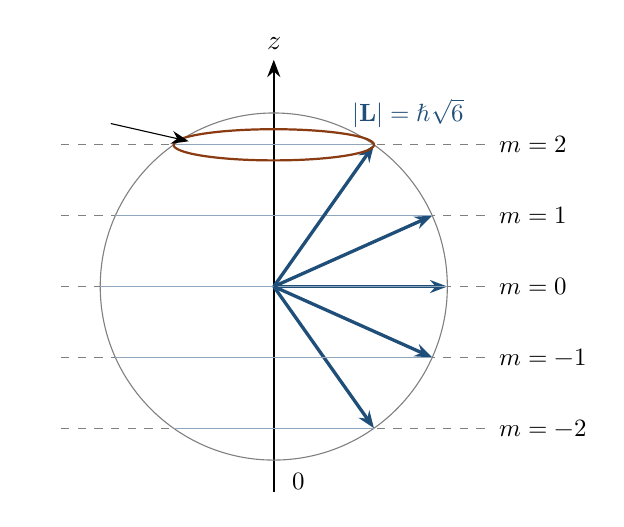
\begin{tikzpicture}[scale=0.9]
  \def\R{2.449} % sqrt(6) for l=2
  \draw[->, thick] (0,-2.9) -- (0,3.2) node[above] {$z$};
  \draw[gray] (0,0) circle (\R);
  \foreach \m in {-2,-1,0,1,2} {
     \draw[dashed, gray] (-3.0,\m) -- (3.0,\m);
     \node[right, font=\small] at (3.05,\m) {$m=\m$};
     \pgfmathsetmacro{\x}{sqrt(6-\m*\m)}
     \draw[very thick, accent, ->] (0,0) -- (\x,\m);
     \draw[accent!50] (-\x,\m) -- (\x,\m);
  }
  \node[font=\small, accent] at (1.9,2.45) {$|\vect L|=\hbar\sqrt6$};
  \draw[keycol, thick] (0,2) ellipse ({sqrt(2)} and 0.22);
  \node[font=\small, align=left] at (-2.9,2.6) {конус\\прецессии};
  \draw[->, thin] (-2.3,2.3) -- (-1.2,2.05);
  \node[font=\small] at (0.35,-2.75) {$0$};
\end{tikzpicture}
\caption{Векторная модель для $l=2$: длина вектора момента $\hbar\sqrt{l(l+1)}=\hbar\sqrt6\approx2{,}45\hbar$,
возможные проекции $L_z=m\hbar$, $m=-2,\dots,2$ (единица по оси $z$ — $\hbar$). Для $m=2$ показан конус,
по которому «распределены» неопределённые компоненты $L_x$, $L_y$.}
\label{fig:9:vector}
\end{figure}

\section{Математические выводы}

\begin{derivation}[label=der:9:comm]{коммутатор $[\op L_x,\op L_y]=\ii\hbar\op L_z$}
Используем $[\op x_i,\op p_j]=\ii\hbar\delta_{ij}$, $[\op x_i,\op x_j]=[\op p_i,\op p_j]=0$ и тождество
$[\op A,\op B\op C]=[\op A,\op B]\op C+\op B[\op A,\op C]$.
\[
  [\op L_x,\op L_y]=[\,y\op p_z-z\op p_y,\ z\op p_x-x\op p_z\,]
  =[y\op p_z,z\op p_x]-[y\op p_z,x\op p_z]-[z\op p_y,z\op p_x]+[z\op p_y,x\op p_z].
\]
Второй и третий коммутаторы равны нулю (в них нет сопряжённых пар). В первом не коммутируют
только $\op p_z$ и $z$: $[y\op p_z,z\op p_x]=y\op p_x[\op p_z,z]=-\ii\hbar\,y\op p_x$. В четвёртом:
$[z\op p_y,x\op p_z]=x\op p_y[z,\op p_z]=\ii\hbar\,x\op p_y$. Итого
\[
  [\op L_x,\op L_y]=\ii\hbar(x\op p_y-y\op p_x)=\ii\hbar\op L_z .
\]
Остальные соотношения~\eqref{eq:9:comm} получаются циклической перестановкой $x\to y\to z\to x$.

\emph{Коммутатор с $\op L^2$.} Например,
\begin{align*}
 [\op L^2,\op L_z]&=[\op L_x^2,\op L_z]+[\op L_y^2,\op L_z]
 =\op L_x[\op L_x,\op L_z]+[\op L_x,\op L_z]\op L_x+\op L_y[\op L_y,\op L_z]+[\op L_y,\op L_z]\op L_y\\
 &=-\ii\hbar(\op L_x\op L_y+\op L_y\op L_x)+\ii\hbar(\op L_y\op L_x+\op L_x\op L_y)=0 .
\end{align*}
\end{derivation}

\begin{derivation}[label=der:9:Lz]{$\op L_z=-\ii\hbar\,\partial/\partial\varphi$}
Рассмотрим функцию $\psi(x,y,z)$ как функцию сферических координат. По правилу дифференцирования
сложной функции
\[
  \pdiff{\psi}{\varphi}=\pdiff{\psi}{x}\pdiff{x}{\varphi}+\pdiff{\psi}{y}\pdiff{y}{\varphi}+\pdiff{\psi}{z}\pdiff{z}{\varphi}.
\]
Из $x=r\sin\theta\cos\varphi$, $y=r\sin\theta\sin\varphi$, $z=r\cos\theta$:
$\pdiff{x}{\varphi}=-r\sin\theta\sin\varphi=-y$, $\pdiff{y}{\varphi}=r\sin\theta\cos\varphi=x$, $\pdiff{z}{\varphi}=0$. Следовательно,
\[
  \pdiff{}{\varphi}=x\pdiff{}{y}-y\pdiff{}{x}\quad\Longrightarrow\quad
  \op L_z=-\ii\hbar\Bigl(x\pdiff{}{y}-y\pdiff{}{x}\Bigr)=-\ii\hbar\pdiff{}{\varphi}.
\]
\end{derivation}

\begin{derivation}[label=der:9:eig]{собственные функции и собственные значения $\op L_z$}
Уравнение $-\ii\hbar\,\dd\Phi/\dd\varphi=L_z\Phi$ — линейное первого порядка:
\[
  \frac{\dd\Phi}{\Phi}=\frac{\ii L_z}{\hbar}\dd\varphi\quad\Longrightarrow\quad\Phi(\varphi)=C\,\ee^{\ii L_z\varphi/\hbar}.
\]
\emph{Условие однозначности:} $\Phi(\varphi+2\pi)=\Phi(\varphi)$ $\Rightarrow$ $\ee^{2\pi\ii L_z/\hbar}=1$ $\Rightarrow$
$L_z/\hbar=m$, $m\in\mathbb Z$. Итак, $L_z=m\hbar$.

\emph{Нормировка:} $\int_0^{2\pi}|C|^2\dd\varphi=2\pi|C|^2=1$ $\Rightarrow$ $C=1/\sqrt{2\pi}$.

\emph{Ортогональность:} $\frac{1}{2\pi}\int_0^{2\pi}\ee^{\ii(m-m')\varphi}\dd\varphi=\delta_{mm'}$.

\emph{Эрмитовость} $\op L_z$ на периодических функциях проверяется интегрированием по частям:
внеинтегральный член $[\Phi_1^*\Phi_2]_0^{2\pi}=0$ из-за периодичности. Поэтому собственные значения
действительны, что согласуется с полученным результатом.
\end{derivation}

\begin{derivation}[label=der:9:Y10]{проверка: $Y_{10}\propto\cos\theta$ — собственная функция $\op L^2$ с $l=1$}
$Y_{10}$ не зависит от $\varphi$, поэтому в~\eqref{eq:9:L2} остаётся только $\theta$-часть:
\[
  \frac{1}{\sin\theta}\diff{}{\theta}\Bigl(\sin\theta\diff{\cos\theta}{\theta}\Bigr)
  =\frac{1}{\sin\theta}\diff{}{\theta}\bigl(-\sin^2\theta\bigr)=\frac{-2\sin\theta\cos\theta}{\sin\theta}=-2\cos\theta .
\]
Значит, $\op L^2Y_{10}=-\hbar^2(-2)Y_{10}=2\hbar^2Y_{10}=\hbar^2\cdot1\cdot(1+1)\,Y_{10}$, т.\,е. $l=1$; и
$\op L_zY_{10}=0$, т.\,е. $m=0$. Аналогично для $Y_{11}\propto\sin\theta\,\ee^{\ii\varphi}$:
$\frac{1}{\sin\theta}\frac{\dd}{\dd\theta}(\sin\theta\cos\theta)-\frac{\sin\theta}{\sin^2\theta}=\frac{\cos2\theta-1}{\sin\theta}=-2\sin\theta$ —
снова $L^2=2\hbar^2$, а $L_z=\hbar$.
\end{derivation}

\begin{derivation}[label=der:9:sum]{сумма $\sum_{m=-l}^{l}m^2$}
$\sum_{m=-l}^{l}m^2=2\sum_{m=1}^{l}m^2=2\cdot\frac{l(l+1)(2l+1)}{6}=\frac{l(l+1)(2l+1)}{3}$ — используется в оценке
$\avg{L_z^2}=\hbar^2l(l+1)/3$ выше.
\end{derivation}

\section{Итоговые формулы}

\keyformula{\op{\vect L}=-\ii\hbar\,\vect r\times\nabla,\qquad [\op L_x,\op L_y]=\ii\hbar\op L_z,\qquad [\op L^2,\op L_i]=0}
 {$\op L_i$ — проекции, $\op L^2$ — квадрат момента; циклические перестановки $x\to y\to z$.}
 {орбитальный момент частицы (те же коммутаторы — для любого момента, включая спин).}
 {какие величины одновременно измеримы ($L^2$ и одна проекция).}

\keyformula{\op L_z=-\ii\hbar\pdiff{}{\varphi},\qquad \Phi_m=\frac{\ee^{\ii m\varphi}}{\sqrt{2\pi}},\qquad L_z=m\hbar,\ m\in\mathbb Z}
 {$\varphi$ — азимутальный угол, $m$ — магнитное квантовое число.}
 {однозначная волновая функция (орбитальный момент).}
 {спектр и собственные функции проекции момента.}

\keyformula{L^2=\hbar^2l(l+1),\qquad l=0,1,2,\dots;\qquad m=-l,\dots,l\ \ (2l+1\ \text{значений})}
 {$l$ — орбитальное квантовое число; $Y_{lm}(\theta,\varphi)$ — сферические функции.}
 {без вывода; орбитальный момент.}
 {классификация состояний в центральном поле ($s,p,d,f$); кратность вырождения.}

\section{Физическая интерпретация}

\textbf{Почему квантуется момент.} Требование однозначности $\Psi$ при повороте на $2\pi$ приводит
к $L_z=m\hbar$; дискретность $L^2$ — следствие условий конечности на сфере. Бор постулировал
$L=n\hbar$; квантовая механика даёт другое: $|\vect L|=\hbar\sqrt{l(l+1)}$, причём $l=0$ возможно
(основное состояние водорода имеет нулевой момент).

\textbf{Сохранение момента.} В центральном поле $U(r)$ операторы $\op L^2$ и $\op L_z$ коммутируют с
$\op H$, поэтому их собственные значения — «хорошие» квантовые числа. Энергия не зависит от $m$
(нет выделенного направления) — вырождение кратности $2l+1$. Магнитное поле выделяет ось $z$ и
снимает это вырождение (эффект Зеемана, \tref{t:12}) — отсюда название «магнитное» число.

\textbf{Связь с экспериментом.} Пространственное квантование проекции момента наблюдается в опыте
Штерна--Герлаха и в расщеплении спектральных линий в магнитном поле на $2l+1$ (или $2j+1$) компонент.

\section{Что необходимо знать на экзамене}

\begin{examcheck}
\checkhead{Определения}
\begin{itemize}
 \item $\op{\vect L}=\vect r\times\op{\vect p}$, компоненты в декартовых координатах; квантовые числа $l$, $m$; обозначения $s,p,d,f$.
\end{itemize}
\checkhead{Формулы}
\begin{itemize}
 \item $[\op L_x,\op L_y]=\ii\hbar\op L_z$ (и циклические), $[\op L^2,\op L_i]=0$;
 \item $\op L_z=-\ii\hbar\,\partial_\varphi$, $\Phi_m=\ee^{\ii m\varphi}/\sqrt{2\pi}$, $L_z=m\hbar$;
 \item $L^2=\hbar^2l(l+1)$, $|m|\le l$, кратность $2l+1$ (без вывода); $Y_{00}$, $Y_{10}$.
\end{itemize}
\checkhead{Выводы}
\begin{itemize}
 \item коммутатор $[\op L_x,\op L_y]$; переход к $\op L_z=-\ii\hbar\,\partial_\varphi$;
 \item решение задачи на собственные значения $\op L_z$ с условием однозначности и нормировкой.
\end{itemize}
\checkhead{Интерпретации}
\begin{itemize}
 \item почему одновременно измеримы лишь $L^2$ и одна проекция; почему $|m|\le l$ и $L>l\hbar$;
 \item векторная модель; классический предел $l\gg1$; связь с сохранением момента и вырождением по $m$.
\end{itemize}
\end{examcheck}

% ======================================================================
\chapter[Уравнение Шредингера для атома водорода]%
        {Уравнение Шредингера для атома водорода}
\label{t:10}
% ======================================================================

\begin{qbox}
\textbf{Билет 10.} Уравнение Шредингера для атома водорода. Волновая функция основного
состояния. Классификация электронных состояний атома водорода (без вывода).
\end{qbox}

\section{Содержание билета}

\textbf{Подтемы:}
\begin{enumerate}
 \item гамильтониан и уравнение Шредингера для электрона в кулоновском поле; приведённая масса;
 \item разделение переменных в сферических координатах; радиальное уравнение, эффективный потенциал;
 \item волновая функция и энергия основного состояния (вывод подстановкой), нормировка,
       радиальное распределение, средние значения;
 \item классификация состояний: квантовые числа $n,l,m$ (и $m_s$), уровни $E_n$, вырождение $n^2$
       \emph{(без вывода)}; обозначения $1s,2p,\dots$
\end{enumerate}

\textbf{Необходимые понятия:} стационарное уравнение Шредингера (\tref{t:06}); оператор
момента импульса и сферические функции (\tref{t:09}); модель Бора (\tref{t:03}); лапласиан
в сферических координатах.

\section{Определения и физические принципы}

\begin{definition}[гамильтониан водородоподобного атома]
В системе центра масс (ядро заряда $Ze$, электрон; приведённая масса $\mu\approx\mel$):
\begin{equation}\label{eq:10:H}
  \op H=-\frac{\hbar^2}{2\mu}\nabla^2-\frac{Ze^2}{r}.
\end{equation}
Учитывается только кулоновское притяжение; спин, релятивистские эффекты и размер ядра не учтены.
\end{definition}

\begin{definition}[квантовые числа атома водорода]
\emph{Главное} $n=1,2,\dots$ (определяет энергию); \emph{орбитальное} $l=0,\dots,n-1$ (квадрат момента
$\hbar^2l(l+1)$); \emph{магнитное} $m=-l,\dots,l$ (проекция $L_z=m\hbar$); \emph{спиновое} $m_s=\pm\frac12$.
\emph{Радиальное} квантовое число $n_r=n-l-1$ — число узлов радиальной функции.
\end{definition}

\emph{Физический смысл.} В центральном поле сохраняются энергия, $L^2$ и $L_z$; их операторы попарно
коммутируют, поэтому стационарные состояния можно нумеровать одновременно значениями $E$, $l$, $m$.
Электрон описывается не орбитой, а распределением плотности вероятности («электронным облаком»).

\emph{Область применимости.} Нерелятивистское приближение: поправки порядка $(Z\alpha)^2$ (тонкая
структура), радиационные поправки (лэмбовский сдвиг), сверхтонкая структура (взаимодействие с
магнитным моментом ядра) — малы и здесь не рассматриваются.

\section{Основная теория}

\subsection{Уравнение Шредингера и разделение переменных}

Стационарное уравнение
\begin{equation}\label{eq:10:sse}
  -\frac{\hbar^2}{2\mu}\nabla^2\psi-\frac{Ze^2}{r}\psi=E\psi .
\end{equation}
Лапласиан в сферических координатах выражается через $\op L^2$ (\tref{t:09}):
\begin{equation}\label{eq:10:lap}
  \nabla^2=\frac{1}{r^2}\pdiff{}{r}\Bigl(r^2\pdiff{}{r}\Bigr)-\frac{\op L^2}{\hbar^2r^2}.
\end{equation}
Поэтому
\(
  \op H=-\frac{\hbar^2}{2\mu}\frac{1}{r^2}\pdiff{}{r}\bigl(r^2\pdiff{}{r}\bigr)+\frac{\op L^2}{2\mu r^2}-\frac{Ze^2}{r}
\)
и решение ищется в виде
\begin{equation}\label{eq:10:sep}
  \psi_{nlm}(r,\theta,\varphi)=R_{nl}(r)\,Y_{lm}(\theta,\varphi).
\end{equation}
Подставив и использовав $\op L^2Y_{lm}=\hbar^2l(l+1)Y_{lm}$, получаем \emph{радиальное уравнение}
\begin{equation}\label{eq:10:radial}
  -\frac{\hbar^2}{2\mu}\frac{1}{r^2}\diff{}{r}\Bigl(r^2\diff{R}{r}\Bigr)
  +\Bigl[\frac{\hbar^2l(l+1)}{2\mu r^2}-\frac{Ze^2}{r}\Bigr]R=ER .
\end{equation}
С подстановкой $R=u/r$ оно сводится к одномерному уравнению
$-\frac{\hbar^2}{2\mu}u''+U_{\text{эфф}}(r)u=Eu$ с граничным условием $u(0)=0$ и
\begin{equation}\label{eq:10:Ueff}
  U_{\text{эфф}}(r)=-\frac{Ze^2}{r}+\frac{\hbar^2l(l+1)}{2\mu r^2}.
\end{equation}
Второй член — \emph{центробежная энергия}: при $l\neq0$ она отталкивает электрон от ядра (рис.~\ref{fig:10:Ueff}).
Связанные состояния существуют при $E<0$.

\begin{figure}[htbp]
\centering
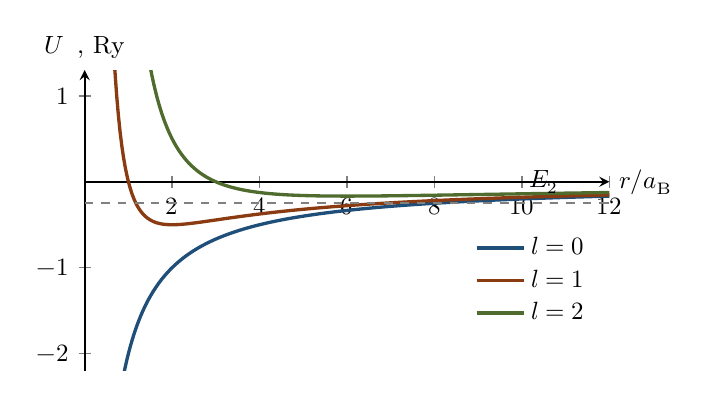
\begin{tikzpicture}
\begin{axis}[width=0.68\linewidth, height=5.4cm, axis lines=middle, xlabel={$r/\aB$}, ylabel={$U_{\text{эфф}}$, Ry},
   xmin=0, xmax=12, ymin=-2.2, ymax=1.3, samples=300, restrict y to domain=-3:2,
   xlabel style={at={(ticklabel* cs:1)}, anchor=west}, ylabel style={at={(ticklabel* cs:1)}, anchor=south},
   legend style={font=\small, draw=none, at={(0.98,0.30)}, anchor=east}]
  \addplot[very thick, accent, domain=0.3:12] {-2/x};
  \addlegendentry{$l=0$}
  \addplot[very thick, keycol, domain=0.3:12] {-2/x + 2/x^2};
  \addlegendentry{$l=1$}
  \addplot[very thick, dercol, domain=0.5:12] {-2/x + 6/x^2};
  \addlegendentry{$l=2$}
  \addplot[gray, dashed, domain=0:12] {-1/4};
  \node[font=\small, anchor=south] at (axis cs:10.5,-0.25) {$E_2$};
\end{axis}
\end{tikzpicture}
\caption{Эффективный потенциал~\eqref{eq:10:Ueff} для $Z=1$ в единицах $\Ry=e^2/2\aB$
($U_{\text{эфф}}/\Ry=-2/\rho+l(l+1)/\rho^2$, $\rho=r/\aB$). Центробежный барьер при $l\neq0$
выталкивает электрон от ядра.}
\label{fig:10:Ueff}
\end{figure}

\subsection{Основное состояние}

Основное состояние сферически симметрично ($l=m=0$) и не имеет узлов. Подстановка $\psi=C\ee^{-r/a}$
(вывод~\ref{der:10:ground}) даёт
\begin{equation}\label{eq:10:psi100}
  \psi_{100}(r)=\frac{1}{\sqrt{\pi a^3}}\,\ee^{-r/a},\qquad
  a=\frac{\hbar^2}{\mu Ze^2},\qquad E_1=-\frac{\mu Z^2e^4}{2\hbar^2}.
\end{equation}
При $Z=1$, $\mu=\mel$: $a=\aB=0{,}529$~Å, $E_1=-13{,}6$~эВ — те же значения, что в модели Бора.
\emph{Радиальная плотность вероятности} (вероятность найти электрон в сферическом слое $(r,r+\dd r)$):
\begin{equation}\label{eq:10:wr}
  w(r)\,\dd r=|\psi_{100}|^2\,4\pi r^2\dd r=\frac{4r^2}{a^3}\ee^{-2r/a}\dd r ,
\end{equation}
максимальна при $r=a$ — наиболее вероятное расстояние совпадает с боровским радиусом. При
этом $\avg r=\frac32a$, а сама плотность $|\psi|^2$ максимальна в центре ($r=0$). Средние энергии:
$\avg U=-Ze^2/a=2E_1$, $\avg T=-E_1$ (вывод~\ref{der:10:means}) — теорема вириала для кулоновского поля.

\subsection{Классификация состояний (без вывода)}

\begin{principle}{Спектр атома водорода (без вывода)}
Решение радиального уравнения~\eqref{eq:10:radial}, конечное при $r=0$ и убывающее при $r\to\infty$,
существует при
\begin{equation}\label{eq:10:En}
  E_n=-\frac{\mu Z^2e^4}{2\hbar^2n^2}=-\frac{Z^2\Ry}{n^2}\frac{\mu}{\mel},\qquad n=n_r+l+1=1,2,\dots,
\end{equation}
где $n_r=0,1,\dots$ — число узлов $R_{nl}$. При данном $n$: $l=0,1,\dots,n-1$; при данном $l$: $m=-l,\dots,l$.
\end{principle}

\paragraph{Вырождение.} Энергия зависит только от $n$. Число состояний с данным $n$:
\begin{equation}\label{eq:10:deg}
  g_n=\sum_{l=0}^{n-1}(2l+1)=n^2\qquad(2n^2\ \text{с учётом спина}).
\end{equation}
Вырождение по $m$ — следствие сферической симметрии (общее для любого центрального поля).
Вырождение по $l$ — особенность кулоновского поля $1/r$ («случайное» вырождение, связанное с
дополнительной сохраняющейся величиной — вектором Рунге--Ленца). В некулоновском поле, например
для валентного электрона щелочного атома, уровни с разными $l$ расщепляются (квантовый дефект,
\tref{t:03}).

\paragraph{Спектроскопические обозначения.} Состояние записывают как $n$ и букву для $l$:
\begin{center}
\begin{tabular}{@{}lccccc@{}}
\toprule
$n$ & $l=0$ & $l=1$ & $l=2$ & $l=3$ & $g_n$ (без спина)\\
\midrule
1 & $1s$ & & & & 1\\
2 & $2s$ & $2p$ & & & 4\\
3 & $3s$ & $3p$ & $3d$ & & 9\\
4 & $4s$ & $4p$ & $4d$ & $4f$ & 16\\
\bottomrule
\end{tabular}
\end{center}

\paragraph{Радиальные функции нижних состояний} ($Z=1$, $\rho=r/a$, нормировка $\int_0^\infty R^2r^2\dd r=1$):
\[
  R_{10}=\frac{2}{a^{3/2}}\ee^{-\rho},\qquad
  R_{20}=\frac{1}{\sqrt2\,a^{3/2}}\Bigl(1-\frac\rho2\Bigr)\ee^{-\rho/2},\qquad
  R_{21}=\frac{1}{2\sqrt6\,a^{3/2}}\,\rho\,\ee^{-\rho/2}.
\]
Общие свойства: $R_{nl}\propto r^l$ при $r\to0$ (центробежный барьер вытесняет электрон из центра,
поэтому лишь $s$-электроны имеют ненулевую плотность в ядре); $R_{nl}\propto\ee^{-Zr/na}$ при $r\to\infty$;
характерный размер растёт как $n^2a/Z$ (рис.~\ref{fig:10:radial}).

\begin{figure}[htbp]
\centering
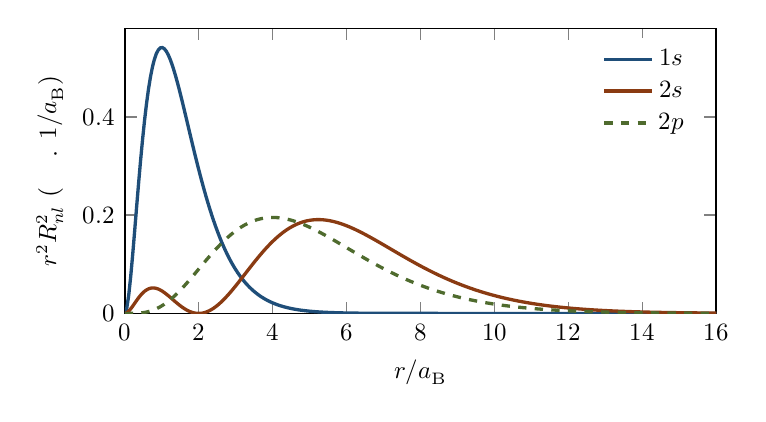
\begin{tikzpicture}
\begin{axis}[width=0.75\linewidth, height=5.2cm, xlabel={$r/\aB$}, ylabel={$r^2R_{nl}^2$ (в ед. $1/\aB$)},
   xmin=0, xmax=16, ymin=0, ymax=0.58, samples=300,
   legend style={font=\small, draw=none}, legend pos=north east]
  \addplot[very thick, accent, domain=0:16] {4*x^2*exp(-2*x)};
  \addlegendentry{$1s$}
  \addplot[very thick, keycol, domain=0:16] {0.5*x^2*(1-x/2)^2*exp(-x)};
  \addlegendentry{$2s$}
  \addplot[very thick, dercol, dashed, domain=0:16] {(1/24)*x^4*exp(-x)};
  \addlegendentry{$2p$}
\end{axis}
\end{tikzpicture}
\caption{Радиальные плотности вероятности $w(r)=r^2R_{nl}^2$ для состояний $1s$, $2s$, $2p$ атома водорода
(расчёт по приведённым формулам). Максимум $1s$ — при $r=\aB$, максимум $2p$ — при $r=4\aB$ (как радиус
второй боровской орбиты); у $2s$ — один радиальный узел при $r=2\aB$.}
\label{fig:10:radial}
\end{figure}

\paragraph{Правила отбора и спектр.} Для электрических дипольных переходов $\Delta l=\pm1$,
$\Delta m=0,\pm1$; $\Delta n$ — любое. Частоты переходов даются той же формулой Ридберга, что и в
модели Бора. Состояние $2s$ не может распасться в $1s$ с испусканием одного фотона
($\Delta l=0$) — оно метастабильно (время жизни $\approx0{,}12$~с, распад с испусканием двух фотонов).

\section{Математические выводы}

\begin{derivation}[label=der:10:ground]{энергия и волновая функция основного состояния}
\emph{Шаг 1.} Для $l=0$ функция зависит только от $r$, и по~\eqref{eq:10:lap}
$\nabla^2\psi=\psi''+\frac2r\psi'$. Уравнение~\eqref{eq:10:sse}:
\[
  -\frac{\hbar^2}{2\mu}\Bigl(\psi''+\frac2r\psi'\Bigr)-\frac{Ze^2}{r}\psi=E\psi .
\]
\emph{Шаг 2 (асимптотика).} При $r\to\infty$ остаётся $\psi''\approx-\frac{2\mu E}{\hbar^2}\psi$; при $E<0$
убывающее решение $\psi\sim\ee^{-\varkappa r}$, $\varkappa=\sqrt{-2\mu E}/\hbar$. Пробуем $\psi=C\ee^{-r/a}$.

\emph{Шаг 3 (подстановка).} $\psi'=-\psi/a$, $\psi''=\psi/a^2$:
\[
  -\frac{\hbar^2}{2\mu}\Bigl(\frac{1}{a^2}-\frac{2}{ar}\Bigr)-\frac{Ze^2}{r}=E
  \quad\Longleftrightarrow\quad
  \Bigl(\frac{\hbar^2}{\mu a}-Ze^2\Bigr)\frac1r=E+\frac{\hbar^2}{2\mu a^2}.
\]
\emph{Шаг 4.} Равенство при всех $r$ возможно, только если обе части равны нулю:
\[
  \frac{\hbar^2}{\mu a}=Ze^2\ \Rightarrow\ a=\frac{\hbar^2}{\mu Ze^2};\qquad
  E=-\frac{\hbar^2}{2\mu a^2}=-\frac{\hbar^2}{2\mu}\cdot\frac{\mu^2Z^2e^4}{\hbar^4}=-\frac{\mu Z^2e^4}{2\hbar^2}.
\]
\emph{Шаг 5 (нормировка).} С интегралом $\int_0^\infty r^n\ee^{-\beta r}\dd r=n!/\beta^{n+1}$:
\[
  \int|\psi|^2\dd V=|C|^2\int_0^\infty\ee^{-2r/a}4\pi r^2\dd r=4\pi|C|^2\frac{2!}{(2/a)^3}=\pi a^3|C|^2=1
  \ \Rightarrow\ C=\frac{1}{\sqrt{\pi a^3}}.
\]
Функция не имеет узлов, поэтому это действительно основное состояние.
\end{derivation}

\begin{derivation}[label=der:10:means]{наиболее вероятное расстояние, $\avg r$, средние энергии}
\emph{Наиболее вероятное $r$.} $w(r)\propto r^2\ee^{-2r/a}$; $\dfrac{\dd w}{\dd r}\propto\bigl(2r-\dfrac{2r^2}{a}\bigr)\ee^{-2r/a}=0$ $\Rightarrow$ $r=a$.

\emph{Среднее расстояние.}
$\avg r=\dfrac{4}{a^3}\displaystyle\int_0^\infty r^3\ee^{-2r/a}\dd r=\dfrac{4}{a^3}\cdot\dfrac{3!}{(2/a)^4}=\dfrac{4\cdot6\,a^4}{16\,a^3}=\dfrac32a .$

\emph{Средняя потенциальная энергия.}
$\avg{1/r}=\dfrac{4}{a^3}\displaystyle\int_0^\infty r\,\ee^{-2r/a}\dd r=\dfrac{4}{a^3}\cdot\dfrac{a^2}{4}=\dfrac1a$, поэтому
$\avg U=-Ze^2\avg{1/r}=-\dfrac{Ze^2}{a}=-\dfrac{\mu Z^2e^4}{\hbar^2}=2E_1$.

\emph{Средняя кинетическая энергия.} $\avg T=E_1-\avg U=-E_1=\dfrac{\mu Z^2e^4}{2\hbar^2}>0$. Соотношение
$2\avg T=-\avg U$ — квантовая теорема вириала для потенциала $\propto1/r$.

\emph{Вероятность найти электрон дальше $r=2a$} (оценка «размытости» облака):
$\int_{2a}^\infty w\,\dd r=\ee^{-4}(1+4+8)=13\ee^{-4}\approx0{,}24$.
\end{derivation}

\begin{derivation}[label=der:10:deg]{кратность вырождения $n^2$}
$g_n=\sum_{l=0}^{n-1}(2l+1)=2\cdot\frac{(n-1)n}{2}+n=n^2-n+n=n^2$. С учётом двух проекций спина — $2n^2$:
это ёмкость электронной оболочки с данным $n$ (2, 8, 18, 32), важная для периодической системы (\tref{t:13}).
\end{derivation}

\begin{derivation}[label=der:10:2p]{проверка: $R_{21}\propto r\ee^{-r/2a}$ даёт $E_2=E_1/4$}
Для $l=1$ в уравнении~\eqref{eq:10:radial} ($Z=1$) положим $R=r\ee^{-r/b}$. Тогда
$R'=(1-r/b)\ee^{-r/b}$, $\frac{1}{r^2}(r^2R')'=\bigl(\frac2r-\frac4b+\frac{r}{b^2}\bigr)\ee^{-r/b}$. Подстановка и деление на $\ee^{-r/b}$:
\[
  -\frac{\hbar^2}{2\mu}\Bigl(\frac2r-\frac4b+\frac{r}{b^2}\Bigr)+\frac{\hbar^2}{\mu r}-e^2=Er .
\]
Члены $\propto1/r$ сокращаются автоматически (в этом роль центробежного слагаемого). Члены без $r$:
$\frac{2\hbar^2}{\mu b}=e^2$ $\Rightarrow$ $b=2\aB$. Члены $\propto r$: $E=-\frac{\hbar^2}{2\mu b^2}=-\frac{\hbar^2}{8\mu\aB^2}=\frac{E_1}{4}$ — в согласии с $E_n=E_1/n^2$
при $n=2$. Максимум $w=r^2R^2\propto r^4\ee^{-r/\aB}$ — при $r=4\aB$.
\end{derivation}

\section{Итоговые формулы}

\keyformula{\op H=-\frac{\hbar^2}{2\mu}\nabla^2-\frac{Ze^2}{r},\qquad \psi_{nlm}=R_{nl}(r)Y_{lm}(\theta,\varphi)}
 {$\mu$ — приведённая масса, $Ze$ — заряд ядра, $Y_{lm}$ — сферические функции.}
 {нерелятивистское приближение, точечное ядро, без спина.}
 {постановка задачи; разделение на радиальную и угловую части.}

\keyformula{\psi_{100}=\frac{\ee^{-r/a}}{\sqrt{\pi a^3}},\quad a=\frac{\hbar^2}{\mu Ze^2},\quad E_1=-\frac{\mu Z^2e^4}{2\hbar^2},\quad r_{\text{вер}}=a,\ \avg r=\tfrac32a}
 {$a$ — боровский радиус (для $Z=1$, $\mu=\mel$: $0{,}529$~Å), $E_1=-13{,}6$~эВ.}
 {основное состояние ($n=1$, $l=m=0$).}
 {распределение электрона, размер атома, энергия ионизации.}

\keyformula{E_n=-\frac{Z^2\Ry}{n^2},\quad n=n_r+l+1,\quad l\le n-1,\quad |m|\le l,\quad g_n=n^2\ (2n^2)}
 {$n$, $l$, $m$ — главное, орбитальное, магнитное квантовые числа; $n_r$ — число радиальных узлов.}
 {кулоновское поле (без вывода).}
 {классификация состояний, кратность вырождения, ёмкость оболочек.}

\section{Физическая интерпретация}

\textbf{Сравнение с моделью Бора.} Уровни $E_n$ совпадают, но физическая картина иная: вместо
орбит — распределения вероятности; основное состояние имеет $L=0$ (у Бора $L=\hbar$); боровский
радиус — наиболее вероятное, а не точное расстояние. Совпадение радиусов $n^2\aB$ с максимумами
$w(r)$ имеет место только для состояний с $l=n-1$ (без радиальных узлов).

\textbf{Предельные случаи и масштабы.} Размер $\propto n^2/Z$, энергия связи $\propto Z^2/n^2$. Электроны
$s$-состояний имеют конечную плотность в ядре $|\psi(0)|^2=Z^3/(\pi n^3a^3)$ — это определяет
сверхтонкое расщепление, вероятность электронного захвата (\tref{t:20}) и изотопический «объёмный» сдвиг.

\textbf{Эксперимент.} Спектр водорода — один из наиболее точно измеренных: формула~\eqref{eq:10:En}
выполняется до $\sim10^{-5}$; оставшиеся расхождения (тонкая структура, лэмбовский сдвиг) объясняются
релятивистской теорией и квантовой электродинамикой.

\section{Что необходимо знать на экзамене}

\begin{examcheck}
\checkhead{Определения}
\begin{itemize}
 \item гамильтониан атома водорода, приведённая масса; квантовые числа $n,l,m,m_s$ и их допустимые значения;
 \item эффективный потенциал и центробежный барьер; радиальная плотность вероятности.
\end{itemize}
\checkhead{Формулы}
\begin{itemize}
 \item $\psi_{100}=\ee^{-r/a}/\sqrt{\pi a^3}$, $a=\hbar^2/\mu Ze^2$, $E_1=-\mu Z^2e^4/2\hbar^2$;
 \item $E_n=-Z^2\Ry/n^2$, $n=n_r+l+1$, вырождение $n^2$ ($2n^2$) — без вывода; обозначения $1s$, $2p$, \ldots
\end{itemize}
\checkhead{Выводы}
\begin{itemize}
 \item подстановка $C\ee^{-r/a}$ в уравнение Шредингера (шаги 1--4), нормировка;
 \item $r_{\text{вер}}=a$, $\avg r=\frac32a$, $\avg U=2E$, $\avg T=-E$; сумма $\sum(2l+1)=n^2$.
\end{itemize}
\checkhead{Интерпретации}
\begin{itemize}
 \item происхождение вырождения по $m$ и по $l$; почему у щелочных атомов вырождение по $l$ снято;
 \item отличия от модели Бора; плотность $s$-электронов в ядре; правила отбора и метастабильность $2s$.
\end{itemize}
\end{examcheck}

% ======================================================================
\chapter[Ротатор. Вращательные и колебательные уровни молекул]%
        {Ротатор. Вращательные и колебательные уровни молекул}
\label{t:11}
% ======================================================================

\begin{qbox}
\textbf{Билет 11.} Уровни энергии плоского и пространственного ротатора. Вращательные и
колебательные уровни молекул.
\end{qbox}

\section{Содержание билета}

\textbf{Подтемы:}
\begin{enumerate}
 \item плоский ротатор: гамильтониан, уровни, волновые функции, вырождение;
 \item пространственный ротатор: уровни $E_J=\hbar^2J(J+1)/2I$, вырождение;
 \item двухатомная молекула: разделение электронного, колебательного и вращательного движений; оценки масштабов энергий;
 \item вращательный спектр (правило отбора, эквидистантные линии), колебательные уровни, ангармонизм, энергия диссоциации;
 \item колебательно-вращательный спектр (P- и R-ветви); проявления в теплоёмкости газов.
\end{enumerate}

\textbf{Необходимые понятия:} оператор момента импульса и его собственные значения
(\tref{t:09}); гармонический осциллятор (\tref{t:08}); приведённая масса (\tref{t:03}).

\section{Определения и физические принципы}

\begin{definition}[ротатор]
\emph{Ротатор} — система, способная только вращаться вокруг неподвижной точки (центра масс) с
фиксированным моментом инерции $I$. \emph{Плоский} ротатор вращается в фиксированной плоскости
(одна угловая координата $\varphi$); \emph{пространственный} — вращается произвольно (углы $\theta,\varphi$).
Модель «жёсткой гантели»: две массы $m_1$, $m_2$ на расстоянии $r_0$, $I=\mu r_0^2$, $\mu=m_1m_2/(m_1+m_2)$.
\end{definition}

\begin{definition}[вращательная постоянная]
\begin{equation}
  B=\frac{\hbar^2}{2I}\qquad\Bigl(\text{в спектроскопии также } \tilde B=\frac{B}{hc}=\frac{\hbar}{4\pi cI}\ \text{в см}^{-1}\Bigr).
\end{equation}
\end{definition}

\emph{Физический смысл.} Классически энергия вращения $E=L^2/2I$ непрерывна. В квантовой
механике $L^2$ квантуется, поэтому квантуется и энергия вращения. \emph{Область применимости:}
модель жёсткого ротатора справедлива, когда центробежное растяжение связи мало
($BJ(J+1)\ll\hbar\omega_{\text{кол}}$) и вращение не возбуждает электронные переходы.

\section{Основная теория}

\subsection{Плоский ротатор}

Кинетическая энергия вращения в плоскости $E=L_z^2/2I$, поэтому гамильтониан
\begin{equation}\label{eq:11:Hplane}
  \op H=\frac{\op L_z^2}{2I}=-\frac{\hbar^2}{2I}\diff{^2}{\varphi^2}.
\end{equation}
Собственные функции $\op L_z$ (\tref{t:09}) — одновременно собственные функции $\op H$
(вывод~\ref{der:11:plane}):
\begin{equation}\label{eq:11:Eplane}
  \Phi_m=\frac{\ee^{\ii m\varphi}}{\sqrt{2\pi}},\qquad E_m=\frac{\hbar^2m^2}{2I},\qquad m=0,\pm1,\pm2,\dots
\end{equation}
Уровни с $m\neq0$ \emph{двукратно вырождены} ($\pm m$ — вращение в противоположных направлениях с одинаковой
энергией); основное состояние $m=0$ невырождено и имеет $E=0$ — нулевых «вращательных колебаний» нет,
поскольку координата $\varphi$ циклическая и ограничения на неё нет (в отличие от ямы или осциллятора).

\subsection{Пространственный ротатор}

\begin{equation}\label{eq:11:Hsph}
  \op H=\frac{\op L^2}{2I}\quad\Longrightarrow\quad
  E_J=\frac{\hbar^2}{2I}J(J+1)=BJ(J+1),\qquad J=0,1,2,\dots,
\end{equation}
волновые функции — сферические функции $Y_{JM}(\theta,\varphi)$, кратность вырождения $g_J=2J+1$
($M=-J,\dots,J$) — энергия не зависит от ориентации оси вращения. Для молекул вращательное квантовое
число обозначают $J$. Расстояние между соседними уровнями растёт линейно:
\begin{equation}\label{eq:11:dE}
  E_{J+1}-E_J=2B(J+1).
\end{equation}

\subsection{Двухатомная молекула: иерархия движений}

Молекула — система из ядер (масса $M$) и электронов (масса $\mel\ll M$). Лёгкие электроны движутся
быстро, ядра — медленно; поэтому в нулевом приближении (приближение Борна--Оппенгеймера) электронная
задача решается при неподвижных ядрах, а её энергия $U(r)$ как функция межъядерного расстояния
служит потенциалом для движения ядер (рис.~\ref{fig:11:morse}). Полная энергия
\begin{equation}\label{eq:11:Etot}
  E=E_{\text{эл}}+E_{\text{кол}}+E_{\text{вр}},\qquad
  E_{\text{эл}}:E_{\text{кол}}:E_{\text{вр}}\sim1:\sqrt{\frac{\mel}{M}}:\frac{\mel}{M}
\end{equation}
(вывод~\ref{der:11:scales}). Численно: $E_{\text{эл}}\sim$ единицы эВ (видимый и УФ диапазоны),
$E_{\text{кол}}\sim0{,}1$--$0{,}5$~эВ (инфракрасный), $E_{\text{вр}}\sim10^{-4}$--$10^{-2}$~эВ (далёкий ИК и микроволновый).

\subsection{Колебательные уровни}

Вблизи минимума $r_0$ потенциальной кривой $U(r)\approx U(r_0)+\frac12k(r-r_0)^2$. Относительное движение ядер
вдоль оси молекулы — осциллятор с приведённой массой $\mu$:
\begin{equation}\label{eq:11:vib}
  E_v=\hbar\omega\Bigl(v+\frac12\Bigr),\qquad \omega=\sqrt{\frac{k}{\mu}},\qquad v=0,1,2,\dots
\end{equation}
Реальный потенциал ангармоничен (например, потенциал Морзе $U=D_e(1-\ee^{-\beta(r-r_0)})^2$): с ростом $v$
уровни сгущаются,
\begin{equation}\label{eq:11:anh}
  E_v=\hbar\omega\Bigl(v+\frac12\Bigr)-\hbar\omega x_e\Bigl(v+\frac12\Bigr)^2,\qquad x_e\ll1,
\end{equation}
и сходятся к границе диссоциации. \emph{Энергия диссоциации} из основного состояния
$D_0=D_e-\hbar\omega/2$ меньше глубины ямы $D_e$ на энергию нулевых колебаний. Правило отбора для гармонических
колебаний $\Delta v=\pm1$; ангармонизм допускает слабые обертоны $\Delta v=\pm2,\pm3,\dots$ Колебательный
дипольный спектр есть только у полярных молекул (HCl, CO); у гомоядерных (H$_2$, N$_2$) дипольный момент не
меняется при колебаниях, и ИК-поглощения нет (колебания наблюдаются в комбинационном рассеянии).

\begin{figure}[htbp]
\centering
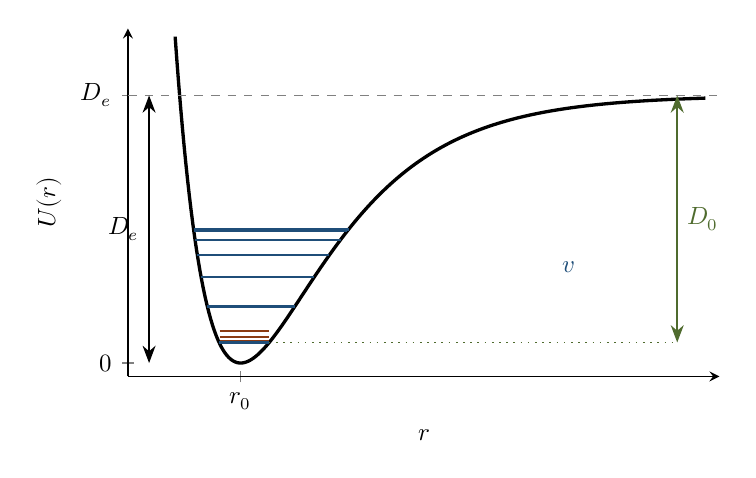
\begin{tikzpicture}
\begin{axis}[width=0.75\linewidth, height=6.0cm, axis lines=left, xlabel={$r$}, ylabel={$U(r)$},
   xmin=0.4, xmax=4.6, ymin=-0.05, ymax=1.25, xtick={1.2}, xticklabels={$r_0$}, ytick={0,1},
   yticklabels={$0$,$D_e$}, samples=300, clip=false]
  \addplot[very thick, domain=0.735:4.5] {(1-exp(-1.6*(x-1.2)))^2};
  \addplot[gray, dashed, domain=0.4:4.6] {1};
  \foreach \v in {0,1,2,3,4,5,6} {
    \pgfmathsetmacro{\Ev}{0.16*(\v+0.5)-0.0128*(\v+0.5)^2}
    \pgfmathsetmacro{\xl}{1.2-ln(1+sqrt(\Ev))/1.6}
    \pgfmathsetmacro{\xr}{1.2-ln(1-sqrt(\Ev))/1.6}
    \edef\tmp{\noexpand\draw[accent, thick] (axis cs:\xl,\Ev) -- (axis cs:\xr,\Ev);}\tmp
  }
  % вращательные подуровни для v=0 (схематично)
  \foreach \J in {1,2,3} { \pgfmathsetmacro{\EJ}{0.0768+0.0035*\J*(\J+1)}
     \edef\tmp{\noexpand\draw[keycol] (axis cs:1.05,\EJ) -- (axis cs:1.40,\EJ);}\tmp }
  \node[font=\small, accent, anchor=west] at (axis cs:2.35,0.36) {колебательные уровни $v$};
  \node[font=\small, anchor=west] at (axis cs:2.6,0.9) {граница диссоциации};
  \draw[<->] (axis cs:0.55,0) -- (axis cs:0.55,1) node[midway, left, font=\small] {$D_e$};
  \draw[<->, dercol] (axis cs:4.3,0.0768) -- (axis cs:4.3,1) node[midway, right, font=\small] {$D_0$};
  \draw[dercol, dotted] (axis cs:1.4,0.0768) -- (axis cs:4.3,0.0768);
\end{axis}
\end{tikzpicture}
\caption{Потенциальная кривая двухатомной молекулы (потенциал Морзе, схема): колебательные уровни
сгущаются к границе диссоциации; $D_0=D_e-\hbar\omega/2$. Около уровня $v=0$ условно показаны вращательные
подуровни (в реальных молекулах они значительно гуще).}
\label{fig:11:morse}
\end{figure}

\subsection{Вращательный спектр}

Переходы между вращательными уровнями одного колебательного состояния возможны для молекул с
постоянным дипольным моментом; правило отбора $\Delta J=\pm1$. Частоты поглощения $J\to J+1$:
\begin{equation}\label{eq:11:rotspec}
  \hbar\omega_J=E_{J+1}-E_J=2B(J+1),\qquad J=0,1,2,\dots
\end{equation}
— эквидистантная последовательность линий с интервалом $2B$ (рис.~\ref{fig:11:spec}). По интервалу
определяют $I$ и межъядерное расстояние $r_0=\sqrt{I/\mu}$. Интенсивности линий определяются
заселённостями $N_J\propto(2J+1)\ee^{-BJ(J+1)/k_{\mathrm B}T}$ — максимум при $J\approx\sqrt{k_{\mathrm B}T/2B}$.

\begin{figure}[htbp]
\centering
\begin{tikzpicture}[xscale=1.25]
  \draw[->] (0,0) -- (9.8,0) node[right] {$\omega$};
  \foreach \J/\h in {0/0.9,1/1.6,2/2.0,3/2.05,4/1.8,5/1.4,6/0.95,7/0.55} {
     \draw[very thick, accent] ({1.1*(\J+1)},0) -- ({1.1*(\J+1)},\h);
  }
  \draw[<->] (1.1,-0.35) -- (2.2,-0.35) node[midway, below, font=\small] {$2B/\hbar$};
  \node[font=\small] at (1.1,2.4) {$0\!\to\!1$};
  \node[font=\small] at (3.3,2.4) {$2\!\to\!3$};
\end{tikzpicture}
\caption{Вращательный спектр поглощения полярной двухатомной молекулы: эквидистантные линии
$\hbar\omega=2B(J+1)$; огибающая интенсивностей определяется больцмановской заселённостью
уровней (схема).}
\label{fig:11:spec}
\end{figure}

\subsection{Колебательно-вращательный спектр}

При переходе $v=0\to1$ одновременно меняется $J$ ($\Delta J=\pm1$ для двухатомных молекул в электронном состоянии $^1\Sigma$,
к которому относится основное состояние большинства двухатомных молекул). При одинаковой $B$ в обоих колебательных состояниях:
\begin{align}
  \text{R-ветвь }(J\to J+1):\quad &\hbar\omega=\hbar\omega_0+2B(J+1),\quad J=0,1,\dots\\
  \text{P-ветвь }(J\to J-1):\quad &\hbar\omega=\hbar\omega_0-2BJ,\quad J=1,2,\dots
\end{align}
Спектр — две серии линий с интервалом $2B$ по обе стороны от $\omega_0$, а на месте $\omega_0$ — провал
(переход $\Delta J=0$ запрещён). Из-за того что во втором колебательном состоянии $r$ в среднем больше,
$B_1<B_0$ — линии R-ветви сгущаются, P-ветви — разрежаются. Изотопический эффект: у H$^{35}$Cl и H$^{37}$Cl
различаются $\mu$, поэтому линии раздвоены ($\omega\propto\mu^{-1/2}$).

\paragraph{Характерные значения.}
\begin{center}
\small
\begin{tabular}{@{}lccc@{}}
\toprule
Молекула & $r_0$, Å & $B$, мэВ & $\hbar\omega$, эВ \\
\midrule
H$_2$ & 0{,}74 & 7{,}5 & 0{,}55 \\
HCl & 1{,}27 & 1{,}3 & 0{,}37 \\
CO & 1{,}13 & 0{,}24 & 0{,}27 \\
\bottomrule
\end{tabular}
\end{center}

\subsection{Теплоёмкость двухатомного газа}

Степени свободы «включаются», когда $k_{\mathrm B}T$ становится сравнимой с расстоянием между уровнями. Для H$_2$
характерные температуры $\Theta_{\text{вр}}=B/k_{\mathrm B}\approx88$~К, $\Theta_{\text{кол}}=\hbar\omega/k_{\mathrm B}\approx6300$~К.
Поэтому при $T\ll\Theta_{\text{вр}}$ $C_V=\frac32R$ (только поступательное движение), при
$\Theta_{\text{вр}}\ll T\ll\Theta_{\text{кол}}$ $C_V=\frac52R$, и лишь при $T\gtrsim\Theta_{\text{кол}}$ $C_V\to\frac72R$.
Классическая теория (равнораспределение) не могла объяснить «вымерзание» степеней свободы.

\section{Математические выводы}

\begin{derivation}[label=der:11:plane]{уровни плоского ротатора}
Стационарное уравнение: $-\dfrac{\hbar^2}{2I}\dfrac{\dd^2\Phi}{\dd\varphi^2}=E\Phi$, т.\,е. $\Phi''+\dfrac{2IE}{\hbar^2}\Phi=0$.
Общее решение $\Phi=A\ee^{\ii\kappa\varphi}+B\ee^{-\ii\kappa\varphi}$, $\kappa=\sqrt{2IE}/\hbar$. Условие однозначности
$\Phi(\varphi+2\pi)=\Phi(\varphi)$ даёт $\ee^{2\pi\ii\kappa}=1$, т.\,е. $\kappa=|m|$, $m$ — целое. Отсюда
\[
  E_m=\frac{\hbar^2m^2}{2I},\qquad \Phi_m=\frac{1}{\sqrt{2\pi}}\ee^{\ii m\varphi}.
\]
Тот же результат сразу следует из $\op H=\op L_z^2/2I$ и $L_z=m\hbar$: собственная функция $\op L_z$ — собственная
функция $\op L_z^2$ с собственным значением $m^2\hbar^2$. Каждому $E_m$ ($m\neq0$) отвечают две независимые функции
$\ee^{\pm\ii|m|\varphi}$ — двукратное вырождение.
\end{derivation}

\begin{derivation}[label=der:11:rigid]{ротатор как частица на сфере}
Пусть частица массы $\mu$ движется по сфере радиуса $r_0$ (жёсткая гантель после отделения центра масс).
Гамильтониан $\op H=-\frac{\hbar^2}{2\mu}\nabla^2$ при фиксированном $r=r_0$ содержит лишь угловую часть лапласиана:
\[
  \op H=-\frac{\hbar^2}{2\mu r_0^2}\Delta_{\theta,\varphi}=\frac{\op L^2}{2\mu r_0^2}=\frac{\op L^2}{2I}.
\]
Собственные значения $\op L^2$ равны $\hbar^2J(J+1)$ (\tref{t:09}), откуда $E_J=\hbar^2J(J+1)/2I$, $g_J=2J+1$.
Классический предел: при $J\gg1$ $E\approx\hbar^2J^2/2I=L^2/2I$ с $L\approx\hbar J$.
\end{derivation}

\begin{derivation}[label=der:11:scales]{оценка соотношения электронных, колебательных и вращательных энергий}
\emph{Электронная энергия.} Электрон локализован в области размера $a\sim\aB$:
$E_{\text{эл}}\sim\hbar^2/(\mel a^2)\sim$ несколько эВ.

\emph{Колебательная энергия.} Сдвиг ядер на расстояние $\sim a$ меняет электронную энергию на величину
порядка $E_{\text{эл}}$, поэтому жёсткость связи $k\sim E_{\text{эл}}/a^2$. Частота колебаний ядер массы $M$:
\[
  \hbar\omega=\hbar\sqrt{\frac kM}\sim\hbar\sqrt{\frac{E_{\text{эл}}}{Ma^2}}
  =\hbar\sqrt{\frac{\hbar^2}{\mel a^2}\cdot\frac{1}{Ma^2}}=\frac{\hbar^2}{\mel a^2}\sqrt{\frac{\mel}{M}}
  =E_{\text{эл}}\sqrt{\frac{\mel}{M}} .
\]
\emph{Вращательная энергия.} $I\sim Ma^2$, $E_{\text{вр}}\sim\dfrac{\hbar^2}{Ma^2}=\dfrac{\hbar^2}{\mel a^2}\dfrac{\mel}{M}=E_{\text{эл}}\dfrac{\mel}{M}$.

При $\mel/M\sim10^{-4}$ (лёгкие молекулы): $E_{\text{эл}}:E_{\text{кол}}:E_{\text{вр}}\sim1:10^{-2}:10^{-4}$.
Эта иерархия оправдывает раздельное рассмотрение трёх типов движения. Попутно: амплитуда нулевых
колебаний $\delta r\sim\sqrt{\hbar/M\omega}\sim a(\mel/M)^{1/4}\sim0{,}1a$ — ядра действительно локализованы.
\end{derivation}

\begin{derivation}[label=der:11:H2]{вращательная постоянная H$_2$}
$\mu=m_p/2$, $r_0=0{,}741$~Å. $I=\mu r_0^2$; в энергетических единицах
\[
  B=\frac{\hbar^2}{2\mu r_0^2}=\frac{(\hbar c)^2}{2\mu c^2r_0^2}=\frac{(1973\ \text{эВ}\cdot\text{Å})^2}{2\cdot469\cdot10^6\ \text{эВ}\cdot(0{,}741\ \text{Å})^2}
  =\frac{3{,}89\cdot10^6}{5{,}15\cdot10^8}\ \text{эВ}\approx7{,}6\cdot10^{-3}\ \text{эВ}.
\]
Интервал между линиями вращательного спектра $2B\approx15$~мэВ соответствует $\lambda=hc/2B\approx0{,}08$~мм
(далёкий ИК). Температура $\Theta_{\text{вр}}=B/k_{\mathrm B}=7{,}6\cdot10^{-3}/8{,}62\cdot10^{-5}\approx88$~К.
\end{derivation}

\begin{derivation}[label=der:11:PR]{P- и R-ветви}
Энергия состояния $E(v,J)=\hbar\omega_0(v+\frac12)+BJ(J+1)$. Переход $(0,J)\to(1,J')$:
\[
  \Delta E=\hbar\omega_0+B\bigl[J'(J'+1)-J(J+1)\bigr].
\]
При $J'=J+1$: $J'(J'+1)-J(J+1)=(J+1)(J+2)-J(J+1)=2(J+1)$ — R-ветвь.
При $J'=J-1$: $(J-1)J-J(J+1)=-2J$ — P-ветвь. При $J'=J$ было бы $\Delta E=\hbar\omega_0$, но такой
переход запрещён правилом отбора $\Delta J=\pm1$ (фотон уносит момент $\hbar$), поэтому в центре спектра — провал.
\end{derivation}

\section{Итоговые формулы}

\keyformula{E_m=\frac{\hbar^2m^2}{2I},\ \ m=0,\pm1,\dots;\qquad E_J=\frac{\hbar^2}{2I}J(J+1),\ \ g_J=2J+1}
 {$I=\mu r_0^2$ — момент инерции, $m$ — проекция момента (плоский ротатор), $J$ — вращательное квантовое число.}
 {жёсткий ротатор (плоский / пространственный).}
 {вращательные уровни молекул.}

\keyformula{\hbar\omega=2B(J+1),\qquad B=\frac{\hbar^2}{2I},\qquad \Delta J=\pm1}
 {$B$ — вращательная постоянная.}
 {полярные молекулы, переходы внутри одного колебательного состояния.}
 {по интервалу $2B$ между линиями — момент инерции и межъядерное расстояние.}

\keyformula{E_v=\hbar\omega\Bigl(v+\frac12\Bigr)-\hbar\omega x_e\Bigl(v+\frac12\Bigr)^2,\qquad \omega=\sqrt{k/\mu},\qquad D_0=D_e-\frac{\hbar\omega}{2}}
 {$v$ — колебательное число, $x_e$ — постоянная ангармонизма, $D_e$ — глубина ямы, $D_0$ — энергия диссоциации.}
 {малый ангармонизм.}
 {колебательный спектр, энергия диссоциации, изотопические эффекты.}

\keyformula{E_{\text{эл}}:E_{\text{кол}}:E_{\text{вр}}\sim1:\sqrt{\mel/M}:\mel/M}
 {$\mel$ — масса электрона, $M$ — масса ядер.}
 {оценка по порядку величины.}
 {обоснование разделения движений; спектральные диапазоны (УФ-видимый, ИК, микроволновый).}

\section{Физическая интерпретация}

\textbf{Структура молекулярных спектров.} Каждый электронный уровень содержит систему колебательных,
а каждый колебательный — систему вращательных подуровней. Поэтому электронные переходы в молекулах
дают не линии, а \emph{полосы} (полосатые спектры), а ИК-переходы — колебательно-вращательные полосы.

\textbf{Зависимость от параметров.} $B\propto1/(\mu r_0^2)$ — тяжёлые молекулы имеют гуще расположенные
уровни; $\omega\propto\sqrt{k/\mu}$ — изотопическое замещение (H$\to$D) уменьшает $\omega$ в $\approx\sqrt2$ раз
и $B$ — в 2 раза (для H$_2$/D$_2$).

\textbf{Связь с термодинамикой.} Квантование объясняет вымерзание вращательных и колебательных
степеней свободы и температурную зависимость теплоёмкости газов — одно из ранних подтверждений
квантовой теории.

\section{Что необходимо знать на экзамене}

\begin{examcheck}
\checkhead{Определения}
\begin{itemize}
 \item плоский и пространственный ротатор, момент инерции, вращательная постоянная; приближение Борна--Оппенгеймера.
\end{itemize}
\checkhead{Формулы}
\begin{itemize}
 \item $E_m=\hbar^2m^2/2I$ (вырождение 2); $E_J=BJ(J+1)$ (вырождение $2J+1$);
 \item $\hbar\omega=2B(J+1)$, $\Delta J=\pm1$; $E_v=\hbar\omega(v+\frac12)$ (+ангармонизм); $D_0=D_e-\hbar\omega/2$;
 \item P- и R-ветви; $E_{\text{эл}}:E_{\text{кол}}:E_{\text{вр}}\sim1:\sqrt{m/M}:m/M$.
\end{itemize}
\checkhead{Выводы}
\begin{itemize}
 \item уровни плоского ротатора из условия однозначности; пространственный ротатор через $\op L^2$;
 \item оценки масштабов энергий; численная оценка $B$ для H$_2$; ветви колебательно-вращательного спектра.
\end{itemize}
\checkhead{Интерпретации}
\begin{itemize}
 \item почему у ротатора нет нулевой энергии, а у осциллятора есть;
 \item спектральные диапазоны; полосатые спектры; вымерзание степеней свободы и теплоёмкость.
\end{itemize}
\end{examcheck}

% ======================================================================
\chapter[Магнитный момент. Опыт Штерна--Герлаха. Спин]%
        {Магнитный момент электрона. Опыт Штерна--Герлаха. Спин}
\label{t:12}
% ======================================================================

\begin{qbox}
\textbf{Билет 12.} Магнитный орбитальный момент электронов, гиромагнитное отношение, $g$-фактор,
магнетон Бора. Опыт Штерна--Герлаха. Спин электрона, спиновый $g$-фактор.
\end{qbox}

\section{Содержание билета}

\textbf{Подтемы:}
\begin{enumerate}
 \item орбитальный магнитный момент: классический вывод, связь с механическим моментом;
 \item гиромагнитное отношение, $g$-фактор, магнетон Бора; квантование проекции магнитного момента;
 \item атом в магнитном поле: энергия, ларморова прецессия, эффект Зеемана (кратко);
 \item опыт Штерна--Герлаха: идея, расчёт отклонения, результат и его интерпретация;
 \item спин электрона: собственный момент, $s=\frac12$, спиновый магнитный момент, $g_s\approx2$; полный момент.
\end{enumerate}

\textbf{Необходимые понятия:} магнитный момент тока $\mu=IS/c$; энергия и сила для диполя в
поле; оператор момента импульса и его собственные значения (\tref{t:09}).

\section{Определения и физические принципы}

\begin{definition}[магнитный момент и гиромагнитное отношение]
Магнитный момент $\vect\mu$ — величина, определяющая энергию $U=-\vect\mu\cdot\vect B$ и момент сил
$\vect M=\vect\mu\times\vect B$, действующие на систему во внешнем магнитном поле. \emph{Гиромагнитное
отношение} $\gamma$ — коэффициент пропорциональности между магнитным и механическим моментами:
$\vect\mu=\gamma\vect L$.
\end{definition}

\begin{definition}[$g$-фактор и магнетон Бора]
Для электрона магнитный момент записывают в виде
\begin{equation}\label{eq:12:g}
  \vect\mu=-g\,\muB\,\frac{\vect J}{\hbar},\qquad
  \muB=\frac{e\hbar}{2\mel c}=9{,}274\cdot10^{-21}\ \frac{\text{эрг}}{\text{Гс}}=5{,}788\cdot10^{-5}\ \frac{\text{эВ}}{\text{Тл}},
\end{equation}
где $\vect J$ — соответствующий механический момент, $g$ — безразмерный $g$-фактор (фактор Ланде).
Для орбитального движения $g_l=1$, для спина $g_s\approx2$. \emph{Магнетон Бора} $\muB$ — естественная единица
магнитного момента электронной оболочки (в СИ $\muB=e\hbar/2\mel$).
\end{definition}

\begin{definition}[спин]
\emph{Спин} — собственный (внутренний) момент импульса частицы, не связанный с её движением в
пространстве. Оператор спина $\op{\vect S}$ подчиняется тем же коммутационным соотношениям, что и $\op{\vect L}$;
$S^2=\hbar^2s(s+1)$, $S_z=m_s\hbar$, $m_s=-s,\dots,s$. Для электрона $s=\frac12$: $|\vect S|=\frac{\sqrt3}{2}\hbar$, $S_z=\pm\frac\hbar2$.
\end{definition}

\emph{Физический смысл.} Магнитные свойства атомов определяются механическими моментами электронов.
Квантование проекции момента ведёт к квантованию проекции магнитного момента — «пространственному
квантованию», непосредственно наблюдаемому в опыте Штерна--Герлаха. Спин — релятивистское по
происхождению (следует из уравнения Дирака) квантовое свойство без классического аналога: модель
«вращающегося шарика» приводит к линейным скоростям поверхности, много большим $c$.

\section{Основная теория}

\subsection{Орбитальный магнитный момент}

Электрон, движущийся по круговой орбите, — ток $I=e/T=ev/2\pi r$. Его магнитный момент
$\mu=IS/c=evr/2c$, а механический момент $L=\mel vr$. Поскольку заряд электрона отрицателен, векторы
направлены противоположно (вывод~\ref{der:12:orb}):
\begin{equation}\label{eq:12:orb}
  \vect\mu_l=-\frac{e}{2\mel c}\vect L,\qquad \gamma_l=-\frac{e}{2\mel c},\qquad g_l=1 .
\end{equation}
Соотношение не зависит от формы орбиты и скорости — оно выполняется для любого движения заряда при
постоянном отношении $e/m$. В квантовой механике~\eqref{eq:12:orb} остаётся верным как операторное
равенство $\op{\vect\mu}_l=-\frac{e}{2\mel c}\op{\vect L}$. Следовательно,
\begin{equation}\label{eq:12:muz}
  \mu_{lz}=-\frac{e}{2\mel c}m\hbar=-\muB m,\quad m=-l,\dots,l;\qquad
  |\vect\mu_l|=\muB\sqrt{l(l+1)} .
\end{equation}
Проекция орбитального магнитного момента принимает $2l+1$ значений, кратных $\muB$.

\subsection{Атом в магнитном поле}

\paragraph{Энергия.} В однородном поле $\vect B\parallel z$ энергия $U=-\vect\mu\cdot\vect B=-\mu_zB=\muB Bm$. Уровень
с данным $l$ расщепляется на $2l+1$ равноотстоящих подуровней с интервалом $\muB B$ (\emph{нормальный эффект
Зеемана}). При $B=1$~Тл интервал $\approx5{,}8\cdot10^{-5}$~эВ — много меньше расстояний между уровнями атома.

\paragraph{Ларморова прецессия.} Момент сил $\vect\mu\times\vect B$ вызывает прецессию $\vect L$ вокруг $\vect B$ с частотой
(вывод~\ref{der:12:larmor})
\begin{equation}\label{eq:12:larmor}
  \omega_L=\frac{eB}{2\mel c},\qquad \hbar\omega_L=\muB B .
\end{equation}
Квантовое расщепление уровней на $\hbar\omega_L$ — квантовый аналог классической прецессии.

\paragraph{Сила в неоднородном поле.} В однородном поле на диполь действует только момент сил, в
неоднородном — ещё и сила
\begin{equation}\label{eq:12:force}
  \vect F=\nabla(\vect\mu\cdot\vect B)\quad\Longrightarrow\quad F_z\approx\mu_z\pdiff{B_z}{z}
\end{equation}
(когда поле направлено в основном вдоль $z$, а поперечные компоненты $\vect\mu$ из-за быстрой ларморовой
прецессии усредняются до нуля). Сила пропорциональна проекции $\mu_z$ — это и использовано в опыте
Штерна--Герлаха.

\subsection{Опыт Штерна--Герлаха (1922)}

\paragraph{Схема.} Пучок атомов серебра, испарявшихся в печи ($T\approx1300$~К), коллимировался щелями
и проходил между полюсами магнита специальной формы (один полюс — клин, другой — с желобом),
создающего сильно неоднородное поле с градиентом $\partial B_z/\partial z$ поперёк пучка (рис.~\ref{fig:12:sg}).
За магнитом атомы осаждались на стеклянной пластинке.

\paragraph{Ожидания.} Если ориентации магнитного момента распределены непрерывно (классика), $\mu_z$
принимает любые значения от $-\mu$ до $+\mu$, и след пучка должен размыться в сплошную полосу. Если проекция
квантуется, пучок должен расщепиться на конечное число компонент — по числу значений $\mu_z$.

\paragraph{Результат.} Пучок расщепился на \emph{две} компоненты, симметрично смещённые на расстояния,
соответствующие $\mu_z=\pm\muB$ (вывод~\ref{der:12:sg}). Без поля — одна полоса.

\paragraph{Интерпретация.}
\begin{enumerate}
 \item Опыт прямо доказал \emph{пространственное квантование} — дискретность проекции момента.
 \item Две компоненты невозможно объяснить орбитальным моментом: для него число компонент $2l+1$ нечётно.
       Более того, в основном состоянии серебра (конфигурация $[\mathrm{Kr}]4d^{10}5s^1$) единственный
       внешний электрон находится в $s$-состоянии, $l=0$, и орбитального момента нет вовсе.
 \item Вывод: электрон обладает собственным моментом с $2s+1=2$, т.\,е. $s=\frac12$, и магнитным моментом с
       проекцией $\pm\muB$. Отсюда $g_s=\mu_z/(\muB m_s)=2$. (В 1922~г. результат трактовали в рамках
       модели Бора; правильная интерпретация через спин появилась после 1925~г.)
\end{enumerate}
Аналогичные опыты с атомами водорода в основном состоянии (Фиппс и Тейлор, 1927; $l=0$) также дали две
компоненты, что исключает объяснение особенностями серебра.

\begin{figure}[htbp]
\centering
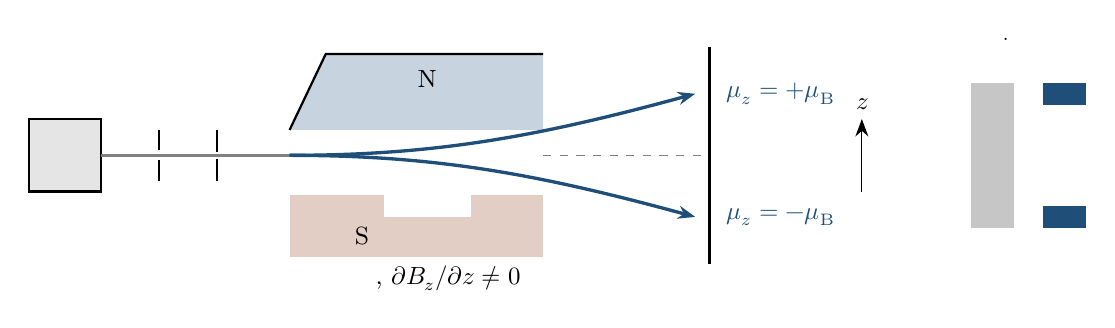
\begin{tikzpicture}[scale=0.92]
  % печь и щели
  \draw[thick, fill=gray!20] (-0.6,-0.5) rectangle (0.4,0.5); \node[below, font=\small] at (-0.1,-0.55) {печь};
  \draw[thick] (1.2,0.35) -- (1.2,0.07); \draw[thick] (1.2,-0.07) -- (1.2,-0.35);
  \draw[thick] (2.0,0.35) -- (2.0,0.05); \draw[thick] (2.0,-0.05) -- (2.0,-0.35);
  \node[below, font=\small] at (1.6,-0.4) {щели};
  % магнит
  \fill[accent!25] (3.0,0.35) -- (3.5,1.4) -- (6.5,1.4) -- (6.5,0.35) -- (6.1,0.35)-- (5.0,0.35) -- cycle;
  \draw[thick] (3.0,0.35) -- (3.5,1.4) -- (6.5,1.4);
  \node[font=\small] at (4.9,1.05) {N};
  \fill[keycol!25] (3.0,-1.4) rectangle (6.5,-0.55);
  \fill[white] (4.3,-0.85) rectangle (5.5,-0.55);
  \node[font=\small] at (4.0,-1.12) {S};
  \node[font=\small] at (4.9,-1.7) {магнит, $\partial B_z/\partial z\neq0$};
  % пучок
  \draw[very thick, gray] (0.4,0) -- (3.0,0);
  \draw[very thick, accent, ->] (3.0,0) .. controls (5.0,0) and (6.4,0.25) .. (8.6,0.85);
  \draw[very thick, accent, ->] (3.0,0) .. controls (5.0,0) and (6.4,-0.25) .. (8.6,-0.85);
  \draw[thin, dashed, gray] (6.5,0) -- (8.7,0);
  % экран
  \draw[very thick] (8.8,-1.5) -- (8.8,1.5); \node[above, font=\small] at (8.8,1.5) {пластинка};
  \node[right, font=\small, accent] at (8.9,0.85) {$\mu_z=+\muB$};
  \node[right, font=\small, accent] at (8.9,-0.85) {$\mu_z=-\muB$};
  \draw[->] (10.9,-0.5) -- (10.9,0.5) node[above, font=\small] {$z$};
  % ожидаемая картина
  \begin{scope}[xshift=12.4cm]
    \node[font=\scriptsize, align=center] at (0.3,1.6) {класс.};
    \fill[gray!45] (0.0,-1.0) rectangle (0.6,1.0);
    \node[font=\scriptsize, align=center] at (1.3,1.6) {опыт};
    \fill[accent] (1.0,0.7) rectangle (1.6,1.0);
    \fill[accent] (1.0,-1.0) rectangle (1.6,-0.7);
  \end{scope}
\end{tikzpicture}
\caption{Схема опыта Штерна--Герлаха. Справа: след пучка при классически непрерывной ориентации
моментов (сплошная полоса) и наблюдаемая картина (две полосы).}
\label{fig:12:sg}
\end{figure}

\subsection{Спин электрона}

Гипотезу спина выдвинули С.~Гаудсмит и Дж.~Уленбек (1925) для объяснения дублетной структуры
спектров щелочных металлов (жёлтая линия натрия — дублет $589{,}0$ и $589{,}6$~нм) и аномального эффекта
Зеемана. Свойства спина электрона:
\begin{align}
  &S^2=\hbar^2s(s+1)=\tfrac34\hbar^2,\qquad S_z=m_s\hbar=\pm\tfrac12\hbar, \label{eq:12:S}\\
  &\vect\mu_s=-g_s\frac{e}{2\mel c}\vect S=-g_s\muB\frac{\vect S}{\hbar},\qquad \mu_{sz}=-g_s\muB m_s\approx\mp\muB,\qquad g_s\approx2 . \label{eq:12:mus}
\end{align}
\emph{Гиромагнитное отношение для спина вдвое больше орбитального}: $\gamma_s=-g_se/2\mel c\approx-e/\mel c$.
Это было подтверждено опытами Эйнштейна--де Гааза (поворот намагничиваемого железного стержня),
давшими для ферромагнетиков $g\approx2$: ферромагнетизм обусловлен спинами, а не орбитальным движением.

Значение $g_s=2$ следует из релятивистского уравнения Дирака (1928). Квантовая электродинамика даёт
поправку: $g_s=2(1+\frac{\alpha}{2\pi}+\dots)=2{,}002\,319\dots$ — одно из наиболее точно проверенных
предсказаний физики.

\paragraph{Описание спина.} Волновая функция электрона зависит не только от $\vect r$, но и от спиновой
переменной $\sigma=\pm\frac12$: $\Psi(\vect r,\sigma)$, или двухкомпонентный столбец (спинор)
$\binom{\psi_+(\vect r)}{\psi_-(\vect r)}$, где $|\psi_\pm|^2$ — плотности вероятности для $S_z=\pm\hbar/2$. Операторы
проекций спина: $\op S_i=\frac\hbar2\sigma_i$ с матрицами Паули
\[
  \sigma_x=\begin{pmatrix}0&1\\1&0\end{pmatrix},\quad
  \sigma_y=\begin{pmatrix}0&-\ii\\\ii&0\end{pmatrix},\quad
  \sigma_z=\begin{pmatrix}1&0\\0&-1\end{pmatrix}.
\]

\paragraph{Полный момент и фактор Ланде.} Полный момент электрона $\vect J=\vect L+\vect S$, $j=l\pm\frac12$
(при $l=0$ только $j=\frac12$). Из-за различия $g_l$ и $g_s$ магнитный момент не коллинеарен $\vect J$; его
проекция на $\vect J$ определяется фактором Ланде (без вывода)
\begin{equation}\label{eq:12:lande}
  g_J=1+\frac{J(J+1)+S(S+1)-L(L+1)}{2J(J+1)},\qquad \mu_{Jz}=-g_J\muB M_J .
\end{equation}
Проверка: при $S=0$ $g_J=1$; при $L=0$ $g_J=2$. Расщепление уровня в слабом поле $\Delta E=g_J\muB BM_J$ —
\emph{аномальный эффект Зеемана}. Спин-орбитальное взаимодействие (энергия магнитного момента спина в
магнитном поле, возникающем в системе покоя электрона из-за его движения относительно ядра) расщепляет
уровни с $l\neq0$ на два ($j=l\pm\frac12$) — тонкая структура, например дублет натрия.

\section{Математические выводы}

\begin{derivation}[label=der:12:orb]{орбитальный магнитный момент}
\emph{Допущения:} электрон (заряд $-e$, масса $\mel$) движется равномерно по окружности радиуса $r$ со
скоростью $v$; гауссова система.

Сила тока — заряд, проходящий через сечение орбиты в единицу времени: $I=e/T=ev/(2\pi r)$.
Магнитный момент плоского витка: $\mu=IS/c=\dfrac{ev}{2\pi r}\cdot\dfrac{\pi r^2}{c}=\dfrac{evr}{2c}$.
Механический момент: $L=\mel vr$. Отношение
\[
  \frac{\mu}{L}=\frac{evr/2c}{\mel vr}=\frac{e}{2\mel c}.
\]
Ток электрона направлен против его скорости, поэтому $\vect\mu$ антипараллелен $\vect L$:
$\vect\mu_l=-\dfrac{e}{2\mel c}\vect L$. Для $L=\hbar$ получаем единицу магнитного момента — магнетон Бора
$\muB=e\hbar/2\mel c$.

\emph{Общность:} для произвольного движения $\vect\mu=\frac{1}{2c}\sum q\,\vect r\times\vect v$, а $\vect L=\sum m\,\vect r\times\vect v$;
при одинаковом $q/m$ для всех частиц $\vect\mu=\frac{q}{2mc}\vect L$.

\emph{Численно:} $\muB=\dfrac{4{,}803\cdot10^{-10}\cdot1{,}0546\cdot10^{-27}}{2\cdot9{,}109\cdot10^{-28}\cdot2{,}998\cdot10^{10}}=9{,}27\cdot10^{-21}$~эрг/Гс.
\end{derivation}

\begin{derivation}[label=der:12:larmor]{ларморова частота}
Уравнение моментов: $\dfrac{\dd\vect L}{\dd t}=\vect\mu\times\vect B=-\dfrac{e}{2\mel c}\vect L\times\vect B=\vect\omega_L\times\vect L$,
где $\vect\omega_L=\dfrac{e\vect B}{2\mel c}$. Уравнение вида $\dot{\vect L}=\vect\omega\times\vect L$ описывает вращение вектора $\vect L$ с
угловой скоростью $\vect\omega$ без изменения его длины и проекции на $\vect\omega$. Следовательно, $\vect L$ прецессирует
вокруг $\vect B$ с частотой $\omega_L=eB/2\mel c$. Энергия $\hbar\omega_L=\frac{e\hbar}{2\mel c}B=\muB B$ совпадает с
расстоянием между зеемановскими подуровнями $\Delta E=\muB B\,\Delta m$ при $\Delta m=1$.
\end{derivation}

\begin{derivation}[label=der:12:sg]{отклонение атомов в опыте Штерна--Герлаха}
\emph{Допущения:} атом движется вдоль $x$ со скоростью $v$; на участке длины $l_1$ внутри магнита действует
постоянная сила $F_z=\mu_z\,\partial B_z/\partial z$; далее — свободный пролёт длины $l_2$ до пластинки.

Внутри магнита (время $t_1=l_1/v$): ускорение $a=F_z/M$,
\[
  z_1=\frac{a t_1^2}{2}=\frac{\mu_z}{2M}\pdiff{B_z}{z}\frac{l_1^2}{v^2},\qquad v_z=at_1 .
\]
На пролёте: $z_2=v_z\frac{l_2}{v}=\frac{\mu_z}{M}\pdiff{B_z}{z}\frac{l_1l_2}{v^2}$. Полное смещение
\[
  z=\frac{\mu_z}{Mv^2}\pdiff{B_z}{z}\Bigl(\frac{l_1^2}{2}+l_1l_2\Bigr).
\]
Смещение пропорционально $\mu_z$: каждой проекции соответствует своя полоса. Для теплового пучка $Mv^2\sim3k_{\mathrm B}T$, поэтому смещение обратно пропорционально температуре печи; разброс скоростей в пучке размывает полосы, но не сливает их.

\emph{Оценка} (только магнит, $l_2=0$): $\partial B/\partial z\approx10^5$~Гс/см ($10^3$~Тл/м), $l_1=3{,}5$~см,
$v\approx5\cdot10^4$~см/с, $M=108\cdot1{,}66\cdot10^{-24}$~г$=1{,}8\cdot10^{-22}$~г, $\mu_z=\muB$:
\[
  z=\frac{9{,}27\cdot10^{-21}\cdot10^5\cdot(3{,}5)^2}{2\cdot1{,}8\cdot10^{-22}\cdot(5\cdot10^4)^2}\ \text{см}
  \approx1{,}3\cdot10^{-2}\ \text{см}=0{,}13\ \text{мм}.
\]
Расстояние между полосами $\sim0{,}2$--$0{,}3$~мм — порядок величины, наблюдавшийся в опыте. Из измеренного
смещения и известных $\partial B/\partial z$, $T$ найдено $|\mu_z|\approx\muB$.
\end{derivation}

\begin{derivation}[label=der:12:gs]{спиновый $g$-фактор из опыта}
Для атома серебра $L=0$, поэтому $\vect\mu=\vect\mu_s$. Наблюдаемые проекции $\mu_z=\pm\muB$, а $S_z=m_s\hbar$, $m_s=\pm\frac12$.
Из $\mu_z=-g_s\muB m_s$: $\muB=g_s\muB\cdot\frac12$ $\Rightarrow$ $g_s=2$. Гиромагнитное отношение
$|\mu_z/S_z|=\muB/(\hbar/2)=e/\mel c$ — вдвое больше орбитального.
\end{derivation}

\section{Итоговые формулы}

\keyformula{\vect\mu_l=-\frac{e}{2\mel c}\vect L,\qquad \mu_{lz}=-\muB m,\qquad \muB=\frac{e\hbar}{2\mel c}}
 {$\vect L$ — орбитальный момент, $m$ — магнитное квантовое число; $g_l=1$.}
 {орбитальное движение электрона (нерелятивистское).}
 {магнитный момент атома, зеемановское расщепление, отклонение в неоднородном поле.}

\keyformula{\vect\mu_s=-g_s\muB\frac{\vect S}{\hbar},\quad g_s\approx2{,}0023,\quad S_z=\pm\frac\hbar2,\quad \mu_{sz}\approx\mp\muB}
 {$\vect S$ — спин, $s=\frac12$.}
 {электрон; $g_s=2$ — по Дираку, поправка $\alpha/\pi$ — КЭД.}
 {спиновый магнетизм, опыт Штерна--Герлаха, ферромагнетизм.}

\keyformula{U=-\vect\mu\cdot\vect B,\qquad F_z=\mu_z\pdiff{B_z}{z},\qquad \omega_L=\frac{eB}{2\mel c}}
 {$\vect B$ — индукция поля, $\omega_L$ — ларморова частота.}
 {сила — в неоднородном поле; поперечные компоненты $\vect\mu$ усреднены прецессией.}
 {энергия в поле, расщепление пучков, прецессия момента.}

\keyformula{g_J=1+\frac{J(J+1)+S(S+1)-L(L+1)}{2J(J+1)},\qquad \Delta E=g_J\muB BM_J}
 {$L,S,J$ — орбитальное, спиновое и полное квантовые числа; $M_J$ — проекция $\vect J$.}
 {$LS$-связь, слабое поле (без вывода).}
 {аномальный эффект Зеемана.}

\section{Физическая интерпретация}

\textbf{Масштабы.} Магнитная энергия $\muB B\approx6\cdot10^{-5}$~эВ при 1~Тл мала по сравнению с
атомными энергиями (эВ) и тепловой энергией при комнатной температуре ($0{,}026$~эВ) — поэтому
парамагнетизм слаб, а ориентационная поляризация моментов требует низких температур или сильных полей.

\textbf{Ядерные моменты.} Для протона вместо $\mel$ стоит $m_p$: ядерный магнетон $\mu_N=e\hbar/2m_pc\approx\muB/1836$.
Магнитные моменты ядер малы, что объясняет малость сверхтонкого расщепления. Аномальные значения
моментов протона ($2{,}79\mu_N$) и нейтрона ($-1{,}91\mu_N$) указывают на их составную (кварковую) структуру.

\textbf{Значение опыта Штерна--Герлаха:} первое прямое доказательство квантования проекции момента и прототип
квантового измерения — каждый атом попадает лишь в одну из полос.

\section{Что необходимо знать на экзамене}

\begin{examcheck}
\checkhead{Определения}
\begin{itemize}
 \item магнитный момент, гиромагнитное отношение, $g$-фактор, магнетон Бора (формула и значение);
 \item спин: $s=\frac12$, $S^2=\frac34\hbar^2$, $S_z=\pm\frac\hbar2$; полный момент $\vect J=\vect L+\vect S$.
\end{itemize}
\checkhead{Формулы}
\begin{itemize}
 \item $\vect\mu_l=-\frac{e}{2\mel c}\vect L$, $g_l=1$; $\vect\mu_s=-g_s\muB\vect S/\hbar$, $g_s\approx2$;
 \item $U=-\vect\mu\vect B$, $F_z=\mu_z\partial B_z/\partial z$, $\omega_L=eB/2\mel c$; формула Ланде (для справки).
\end{itemize}
\checkhead{Выводы}
\begin{itemize}
 \item $\mu/L=e/2\mel c$ для круговой орбиты; ларморова прецессия;
 \item смещение атома в опыте Штерна--Герлаха; $g_s=2$ из наблюдения $\mu_z=\pm\muB$ при $L=0$.
\end{itemize}
\checkhead{Интерпретации}
\begin{itemize}
 \item почему две компоненты доказывают существование спина ($2s+1$ чётно, $l=0$ у Ag и H); опыт Эйнштейна--де Гааза.
\end{itemize}
\end{examcheck}

% ======================================================================
\chapter[Тождественные частицы. Принцип Паули. Сложные атомы. Термы]%
        {Тождественные частицы. Принцип Паули. Сложные атомы и атомные термы}
\label{t:13}
% ======================================================================

\begin{qbox}
\textbf{Билет 13.} Тождественность частиц, бозоны и фермионы, принцип Паули. Сложные атомы.
Электронная конфигурация атома. Атомные термы, спектроскопическая запись состояния атома.
\end{qbox}

\section{Содержание билета}

\textbf{Подтемы:}
\begin{enumerate}
 \item принцип неразличимости тождественных частиц; оператор перестановки; симметричные и антисимметричные состояния;
 \item бозоны и фермионы, связь спина со статистикой;
 \item принцип Паули (из антисимметрии), детерминант Слэтера; обменные эффекты;
 \item многоэлектронный атом: приближение самосогласованного поля, оболочки и подоболочки, порядок заполнения;
 \item электронная конфигурация; периодическая система;
 \item $LS$-связь, атомный терм $^{2S+1}L_J$, правила Хунда; примеры.
\end{enumerate}

\textbf{Необходимые понятия:} спин (\tref{t:12}); квантовые числа атома водорода (\tref{t:10});
сложение моментов; квантовый дефект (\tref{t:03}).

\section{Определения и физические принципы}

\begin{principle}{Принцип тождественности (неразличимости)}
Частицы одного сорта (электроны, протоны, фотоны\,\dots) принципиально неразличимы: перестановка двух
тождественных частиц не меняет физического состояния системы. Все наблюдаемые величины симметричны
относительно перестановок.
\end{principle}

\emph{Физическая причина.} В классике одинаковые частицы можно «пометить» по их траекториям. В квантовой
механике траекторий нет: когда волновые пакеты двух электронов перекрываются, невозможно сказать,
какой из них куда попал после взаимодействия.

\begin{definition}[бозоны и фермионы]
\emph{Бозоны} — частицы с целым спином ($0,1,2,\dots$: фотон, $\pi$-мезон, $W^\pm$, $Z^0$, глюон, бозон Хиггса,
ядро $^4$He); волновая функция системы тождественных бозонов \emph{симметрична} относительно перестановки любых
двух частиц. \emph{Фермионы} — частицы с полуцелым спином ($\frac12,\frac32,\dots$: электрон, протон, нейтрон,
нейтрино, кварки, ядро $^3$He); волновая функция \emph{антисимметрична}.
\end{definition}

\begin{principle}{Принцип Паули (1925)}
В системе тождественных фермионов никакие два фермиона не могут находиться в одном и том же
одночастичном квантовом состоянии. Для электронов в атоме: никакие два электрона не могут иметь
одинаковый набор четырёх квантовых чисел $(n,l,m_l,m_s)$.
\end{principle}

\begin{definition}[конфигурация и терм]
\emph{Электронная конфигурация} — распределение электронов по подоболочкам $nl$ (например, $1s^22s^22p^2$).
\emph{Терм} — состояние атома с определёнными полным орбитальным $L$, полным спиновым $S$ (и, после учёта
спин-орбитального взаимодействия, полным $J$) моментами; записывается как $^{2S+1}L_J$, где $L$ обозначается
буквами $S,P,D,F,G,\dots$ для $L=0,1,2,3,4,\dots$; $2S+1$ — \emph{мультиплетность}.
\end{definition}

\emph{Область применимости.} Одночастичное описание (конфигурации) — приближение независимых электронов в
самосогласованном центральном поле. Схема $LS$-связи справедлива для лёгких и средних атомов, где
электростатическое взаимодействие электронов много сильнее спин-орбитального; для тяжёлых атомов
применяется $jj$-связь.

\section{Основная теория}

\subsection{Симметрия волновой функции}

Пусть $\Psi(1,2)$ — волновая функция двух тождественных частиц, где $1\equiv(\vect r_1,\sigma_1)$. Оператор
перестановки $\op P_{12}\Psi(1,2)=\Psi(2,1)$. Из неразличимости $|\Psi(2,1)|^2=|\Psi(1,2)|^2$, т.\,е.
$\Psi(2,1)=\ee^{\ii\alpha}\Psi(1,2)$. Повторная перестановка возвращает исходное состояние:
$\ee^{2\ii\alpha}=1$, $\ee^{\ii\alpha}=\pm1$ (вывод~\ref{der:13:perm}). Итак, возможны лишь два типа состояний:
\begin{equation}\label{eq:13:sym}
  \Psi(2,1)=+\Psi(1,2)\ \ (\text{симметричные}),\qquad \Psi(2,1)=-\Psi(1,2)\ \ (\text{антисимметричные}).
\end{equation}
Гамильтониан тождественных частиц симметричен, поэтому $\op P_{12}$ коммутирует с $\op H$: тип симметрии
сохраняется во времени. Какой тип реализуется, определяет природа частиц.

\begin{principle}{Теорема о связи спина со статистикой (Паули, 1940; без доказательства)}
Частицы с целым спином описываются симметричными волновыми функциями (подчиняются статистике
Бозе--Эйнштейна), с полуцелым — антисимметричными (статистика Ферми--Дирака). Теорема следует из
релятивистской квантовой теории поля; в нерелятивистской квантовой механике она принимается как постулат.
\end{principle}

Составная частица ведёт себя как бозон, если содержит чётное число фермионов, и как фермион — если нечётное
(при условии, что внутренняя структура не возбуждается): $^4$He (2p+2n+2e) — бозон, $^3$He (2p+1n+2e) — фермион.
Это объясняет различие их свойств при низких температурах (сверхтекучесть $^4$He при 2,17~К, у $^3$He — лишь
при $\sim$мК за счёт образования пар).

\subsection{Принцип Паули как следствие антисимметрии}

Для двух невзаимодействующих частиц в одночастичных состояниях $a$ и $b$ (вывод~\ref{der:13:slater})
\begin{equation}\label{eq:13:2p}
  \Psi_{S,A}(1,2)=\frac{1}{\sqrt2}\bigl[\psi_a(1)\psi_b(2)\pm\psi_a(2)\psi_b(1)\bigr].
\end{equation}
При $a=b$ антисимметричная функция тождественно равна нулю — такое состояние невозможно. Это и есть
принцип Паули. Для $N$ фермионов антисимметричная функция — \emph{детерминант Слэтера}
\begin{equation}\label{eq:13:slater}
  \Psi(1,\dots,N)=\frac{1}{\sqrt{N!}}
  \begin{vmatrix}
   \psi_{a_1}(1)&\psi_{a_1}(2)&\cdots&\psi_{a_1}(N)\\
   \vdots&\vdots&&\vdots\\
   \psi_{a_N}(1)&\psi_{a_N}(2)&\cdots&\psi_{a_N}(N)
  \end{vmatrix},
\end{equation}
обращающийся в нуль при совпадении любых двух строк (одинаковые состояния) или столбцов (одинаковые
координаты и спины: два электрона с одинаковым спином не могут оказаться в одной точке).

\paragraph{Обменные эффекты.} Симметрия волновой функции влияет на пространственное распределение даже без
сил между частицами: при $\vect r_1\to\vect r_2$ пространственно-антисимметричная функция обращается в нуль
(частицы «избегают» друг друга), симметричная — усиливается (бозоны «группируются»). Для электронов
полная функция = координатная $\times$ спиновая, и антисимметрична в целом. Если спины параллельны ($S=1$,
симметричная спиновая часть), координатная часть антисимметрична, электроны в среднем дальше друг от друга,
и кулоновское отталкивание меньше. Поэтому энергия зависит от суммарного спина, хотя гамильтониан спина не
содержит, — \emph{обменное взаимодействие}. Оно объясняет первое правило Хунда, расщепление пара- и
ортогелия (у ортогелия, $S=1$, уровни ниже, чем у парагелия с той же конфигурацией) и ферромагнетизм.

\subsection{Сложные атомы: приближение самосогласованного поля}

Гамильтониан атома с $Z$ электронами (ядро неподвижно)
\[
  \op H=\sum_{i=1}^Z\Bigl(-\frac{\hbar^2}{2\mel}\nabla_i^2-\frac{Ze^2}{r_i}\Bigr)+\sum_{i<j}\frac{e^2}{|\vect r_i-\vect r_j|}
\]
не допускает точного решения. В \emph{приближении центрального (самосогласованного) поля} (Хартри--Фок) каждый
электрон движется в усреднённом сферически симметричном поле ядра и остальных электронов $U(r)$: вблизи
ядра $U\approx-Ze^2/r$, вдали $U\approx-e^2/r$ (ядро экранировано $Z-1$ электронами). Одноэлектронные
состояния характеризуются теми же квантовыми числами $n,l,m_l,m_s$, что и в водороде, но поле некулоновское, поэтому
\emph{энергия зависит от $n$ и $l$}: при данном $n$ состояния с меньшим $l$ глубже проникают к ядру, хуже
экранированы и лежат ниже ($E_{ns}<E_{np}<E_{nd}$).

\paragraph{Оболочки и подоболочки.} Совокупность состояний с данным $n$ — \emph{оболочка} ($K,L,M,N,\dots$ для
$n=1,2,3,4,\dots$), с данными $n,l$ — \emph{подоболочка}. По принципу Паули ёмкость подоболочки $2(2l+1)$
($s$ — 2, $p$ — 6, $d$ — 10, $f$ — 14), оболочки — $2n^2$.

\paragraph{Порядок заполнения} (правило Клечковского) — по возрастанию $n+l$, а при равных $n+l$ — по
возрастанию $n$:
\[
  1s\ \ 2s\ \ 2p\ \ 3s\ \ 3p\ \ 4s\ \ 3d\ \ 4p\ \ 5s\ \ 4d\ \ 5p\ \ 6s\ \ 4f\ \ 5d\ \ 6p\ \ 7s\ \ 5f\ \ 6d\ \ 7p .
\]
Например, $4s$ ($n+l=4$) заполняется раньше $3d$ ($n+l=5$): $s$-электрон сильнее проникает к ядру. Правило
эмпирическое и имеет исключения (Cr: $3d^54s^1$, Cu: $3d^{10}4s^1$ — выгодность наполовину или полностью
заполненной $d$-подоболочки).

\paragraph{Электронные конфигурации (примеры).}
\begin{center}
\small
\begin{tabular}{@{}llll@{}}
\toprule
Атом & Конфигурация & Атом & Конфигурация \\
\midrule
H & $1s$ & Na & $1s^22s^22p^63s=[\mathrm{Ne}]3s$ \\
He & $1s^2$ & Cl & $[\mathrm{Ne}]3s^23p^5$ \\
Li & $1s^22s$ & Ar & $[\mathrm{Ne}]3s^23p^6$ \\
C & $1s^22s^22p^2$ & K & $[\mathrm{Ar}]4s$ \\
N & $1s^22s^22p^3$ & Fe & $[\mathrm{Ar}]3d^64s^2$ \\
O & $1s^22s^22p^4$ & Cu & $[\mathrm{Ar}]3d^{10}4s$ \\
Ne & $1s^22s^22p^6$ & Ag & $[\mathrm{Kr}]4d^{10}5s$ \\
\bottomrule
\end{tabular}
\end{center}

\paragraph{Периодичность.} Химические свойства определяются внешними (валентными) электронами. Атомы с
одинаковой структурой внешней подоболочки имеют сходные свойства: щелочные металлы ($ns^1$, легко
отдают электрон, энергия ионизации 4--5~эВ), галогены ($np^5$), инертные газы (заполненные $np^6$, энергия
ионизации максимальна: 21,6~эВ у Ne, 24,6~эВ у He). Длины периодов 2, 8, 8, 18, 18, 32 — следствие порядка
заполнения подоболочек.

\subsection{Атомные термы и $LS$-связь}

Конфигурация не определяет энергию однозначно: остаточное (нецентральное) взаимодействие электронов
расщепляет её на \emph{термы} с разными $L$ и $S$. В схеме \emph{$LS$-связи} (Рассел--Саундерс) складываются отдельно
орбитальные и спиновые моменты:
\begin{equation}\label{eq:13:LS}
  \vect L=\sum_i\vect l_i,\qquad \vect S=\sum_i\vect s_i,\qquad \vect J=\vect L+\vect S,\qquad
  J=|L-S|,\dots,L+S .
\end{equation}
Спин-орбитальное взаимодействие расщепляет терм на компоненты с разными $J$ — \emph{тонкая структура};
при $L\ge S$ число компонент равно мультиплетности $2S+1$ (отсюда название). \textbf{Запись:}
\[
  ^{2S+1}L_J,\qquad\text{например } ^2S_{1/2},\ ^3P_0,\ ^4S_{3/2},\ ^5D_4 .
\]
\textbf{Заполненные подоболочки} имеют $L=0$, $S=0$ (сумма $m_l$ и сумма $m_s$ равны нулю), т.\,е. терм $^1S_0$.
Поэтому терм атома определяется только электронами незаполненных подоболочек.

\begin{principle}{Правила Хунда (для основного терма)}
\begin{enumerate}[leftmargin=1.4em]
 \item Наименьшую энергию имеет терм с максимальным $S$ (при данной конфигурации).
 \item При данном $S$ — терм с максимальным $L$.
 \item Если подоболочка заполнена менее чем наполовину, ниже лежит компонента с $J=|L-S|$; если более чем
       наполовину — с $J=L+S$.
\end{enumerate}
\end{principle}

Первое правило — следствие обменного взаимодействия (параллельные спины $\Rightarrow$ антисимметричная
координатная функция $\Rightarrow$ меньше отталкивание). Второе — электроны, «вращающиеся» в одну сторону,
реже встречаются. Третье — знак константы спин-орбитальной связи для частиц и «дырок».

\paragraph{Основные термы (примеры, см. вывод~\ref{der:13:hund}).}
\begin{center}
\small
\begin{tabular}{@{}llcccl@{}}
\toprule
Атом & Внешняя подоболочка & $S$ & $L$ & $J$ & Терм \\
\midrule
H, Na, Ag & $ns^1$ & $\frac12$ & 0 & $\frac12$ & $^2S_{1/2}$ \\
He, Be & $ns^2$ & 0 & 0 & 0 & $^1S_0$ \\
B & $2p^1$ & $\frac12$ & 1 & $\frac12$ & $^2P_{1/2}$ \\
C & $2p^2$ & 1 & 1 & 0 & $^3P_0$ \\
N & $2p^3$ & $\frac32$ & 0 & $\frac32$ & $^4S_{3/2}$ \\
O & $2p^4$ & 1 & 1 & 2 & $^3P_2$ \\
F & $2p^5$ & $\frac12$ & 1 & $\frac32$ & $^2P_{3/2}$ \\
Fe & $3d^6$ & 2 & 2 & 4 & $^5D_4$ \\
\bottomrule
\end{tabular}
\end{center}

\paragraph{Полная спектроскопическая запись} состояния атома включает конфигурацию и терм, например
основное состояние углерода $1s^22s^22p^2\ ^3P_0$, натрия $[\mathrm{Ne}]3s\ ^2S_{1/2}$, возбуждённое состояние
натрия $[\mathrm{Ne}]3p\ ^2P_{3/2}$. Дублет натрия — переходы $3p\,^2P_{3/2}\to3s\,^2S_{1/2}$ (589,0~нм) и
$3p\,^2P_{1/2}\to3s\,^2S_{1/2}$ (589,6~нм). Правила отбора для дипольных переходов в $LS$-связи: $\Delta S=0$,
$\Delta L=0,\pm1$, $\Delta J=0,\pm1$ (кроме $0\to0$), $\Delta l=\pm1$ для перескакивающего электрона.

\section{Математические выводы}

\begin{derivation}[label=der:13:perm]{собственные значения оператора перестановки}
По определению $\op P_{12}\Psi(1,2)=\Psi(2,1)$. Применив $\op P_{12}$ дважды, получаем исходную функцию:
$\op P_{12}^2=\op 1$. Если $\op P_{12}\Psi=\lambda\Psi$, то $\op P_{12}^2\Psi=\lambda^2\Psi=\Psi$, откуда $\lambda=\pm1$. Состояние
тождественных частиц должно быть собственной функцией $\op P_{12}$ (иначе перестановка давала бы другое,
физически различимое состояние), поэтому оно либо симметрично, либо антисимметрично. Так как
$[\op P_{12},\op H]=0$, тип симметрии сохраняется со временем.
\end{derivation}

\begin{derivation}[label=der:13:slater]{двухчастичные функции и принцип Паули}
Для невзаимодействующих частиц $\op H=\op h(1)+\op h(2)$, и произведение $\psi_a(1)\psi_b(2)$ — решение с энергией
$\varepsilon_a+\varepsilon_b$. Произведение $\psi_a(2)\psi_b(1)$ — тоже решение с той же энергией (обменное вырождение).
Ни одно из произведений не обладает нужной симметрией при $a\neq b$; строим линейные комбинации:
\[
  \Psi_{S,A}=\frac{1}{\sqrt2}\bigl[\psi_a(1)\psi_b(2)\pm\psi_a(2)\psi_b(1)\bigr],\qquad
  \op P_{12}\Psi_{S,A}=\pm\Psi_{S,A}.
\]
Нормировка ($\psi_a\perp\psi_b$): $\int|\Psi|^2=\frac12(1+1\pm2\cdot0)=1$. Антисимметричную функцию можно записать как
определитель $\frac{1}{\sqrt2}\begin{vmatrix}\psi_a(1)&\psi_a(2)\\\psi_b(1)&\psi_b(2)\end{vmatrix}$. При $a=b$ две строки совпадают и $\Psi_A\equiv0$:
\emph{двух фермионов в одном состоянии быть не может}. Для бозонов при $a=b$ $\Psi_S=\psi_a(1)\psi_a(2)$ —
допустимо, и любое число бозонов может находиться в одном состоянии (основа бозе-конденсации, лазеров).
\end{derivation}

\begin{derivation}[label=der:13:hund]{основные термы по правилам Хунда}
\emph{Алгоритм:} размещаем электроны незаполненной подоболочки по ячейкам $m_l=l,l-1,\dots,-l$, сначала по одному
со спином вверх (максимум $S$), начиная с наибольшего $m_l$ (максимум $L$); затем $M_L=\sum m_l=L$,
$M_S=\sum m_s=S$; $J$ — по третьему правилу.

\emph{Углерод $2p^2$:} $m_l=+1\uparrow$, $0\uparrow$. $S=1$, $L=1+0=1$; подоболочка ($6$ мест) заполнена меньше чем наполовину
$\Rightarrow$ $J=|L-S|=0$. Терм $^3P_0$.

\emph{Азот $2p^3$:} $+1\uparrow,0\uparrow,-1\uparrow$. $S=\frac32$, $L=0$, $J=\frac32$. Терм $^4S_{3/2}$.

\emph{Кислород $2p^4$:} $+1\uparrow\downarrow$, $0\uparrow$, $-1\uparrow$. $S=1$, $L=1+1+0-1=1$; больше половины $\Rightarrow$ $J=L+S=2$.
Терм $^3P_2$. (Эквивалентно: две «дырки» в $p$-подоболочке ведут себя как $p^2$ по $L$ и $S$.)

\emph{Железо $3d^6$:} пять электронов $\uparrow$ на $m_l=2,1,0,-1,-2$ (их $\sum m_l=0$) и шестой $\downarrow$ на $m_l=2$.
$S=\frac52-\frac12=2$, $L=2$; больше половины $\Rightarrow$ $J=4$. Терм $^5D_4$.

\emph{Все термы конфигурации $np^2$} (без доказательства полного перебора): из $\binom62=15$ состояний, допускаемых
принципом Паули, образуются термы $^1S$ (1 состояние), $^1D$ (5) и $^3P$ (9): $1+5+9=15$. Терма $^3D$ нет — он потребовал
бы двух электронов с $m_l=1$ и одинаковыми спинами. Для неэквивалентных электронов ($2p3p$) возможны все
комбинации $L=0,1,2$, $S=0,1$.
\end{derivation}

\begin{derivation}[label=der:13:capacity]{ёмкость подоболочки и оболочки}
При данных $n,l$ квантовое число $m_l$ принимает $2l+1$ значений, $m_s$ — два. По принципу Паули каждый набор
$(n,l,m_l,m_s)$ занят не более чем одним электроном, поэтому ёмкость подоболочки $2(2l+1)$, оболочки
$\sum_{l=0}^{n-1}2(2l+1)=2n^2$ (2, 8, 18, 32).
\end{derivation}

\section{Итоговые формулы}

\keyformula{\Psi(\dots,i,\dots,j,\dots)=\pm\Psi(\dots,j,\dots,i,\dots)}
 {$+$ — бозоны (целый спин), $-$ — фермионы (полуцелый спин); $i\equiv(\vect r_i,\sigma_i)$.}
 {любая система тождественных частиц.}
 {симметрия разрешённых состояний; принцип Паули; статистика.}

\keyformula{\Psi_A=\frac{1}{\sqrt{N!}}\det\bigl[\psi_{a_k}(i)\bigr],\qquad N_{nl}^{\max}=2(2l+1),\quad N_n^{\max}=2n^2}
 {$\psi_{a_k}$ — одночастичные спин-орбитали.}
 {невзаимодействующие фермионы (приближение самосогласованного поля).}
 {принцип Паули; ёмкость подоболочек и оболочек.}

\keyformula{^{2S+1}L_J,\qquad \vect L=\sum\vect l_i,\ \ \vect S=\sum\vect s_i,\ \ J=|L-S|,\dots,L+S}
 {$L$ — полный орбитальный момент ($S,P,D,F$ для $0,1,2,3$), $S$ — полный спин, $J$ — полный момент.}
 {$LS$-связь (лёгкие и средние атомы).}
 {классификация состояний атома; основной терм по правилам Хунда.}

\section{Физическая интерпретация}

\textbf{Без принципа Паули} все электроны оказались бы в состоянии $1s$, атомы разных элементов различались бы
лишь размерами, не было бы периодической системы и химии; вещество было бы неустойчиво к сжатию.
Принцип Паули объясняет оболочечную структуру атомов, устойчивость вещества, свойства металлов
(электронный газ Ферми), белых карликов и нейтронных звёзд (давление вырожденного газа).

\textbf{Энергетическая роль спина.} Гамильтониан без спин-орбитальных членов спина не содержит, но
допустимая симметрия координатной части зависит от суммарного спина. Поэтому энергия термов с разными $S$
различается на величину порядка электростатической (эВ) — много больше магнитной энергии взаимодействия спинов.

\textbf{Эксперимент.} Схема термов проверяется по спектрам: мультиплетность линий, правила отбора, расщепление
в магнитном поле с фактором Ланде $g_J$ (\tref{t:12}). Рентгеновские спектры (закон Мозли) подтверждают оболочечную
структуру внутренних электронов.

\section{Что необходимо знать на экзамене}

\begin{examcheck}
\checkhead{Определения}
\begin{itemize}
 \item принцип тождественности; бозоны, фермионы; связь спина со статистикой; принцип Паули;
 \item приближение самосогласованного поля; оболочка, подоболочка, конфигурация; терм, мультиплетность, $LS$-связь.
\end{itemize}
\checkhead{Формулы}
\begin{itemize}
 \item $\Psi_{S,A}=\frac{1}{\sqrt2}[\psi_a(1)\psi_b(2)\pm\psi_a(2)\psi_b(1)]$; детерминант Слэтера;
 \item ёмкости $2(2l+1)$ и $2n^2$; правило $n+l$; $^{2S+1}L_J$, $J=|L-S|..L+S$.
\end{itemize}
\checkhead{Выводы}
\begin{itemize}
 \item собственные значения $\op P_{12}$ равны $\pm1$; принцип Паули из антисимметрии;
 \item основные термы C, N, O, Fe по правилам Хунда; термы $np^2$.
\end{itemize}
\checkhead{Интерпретации}
\begin{itemize}
 \item обменное взаимодействие и первое правило Хунда; орто- и парагелий;
 \item зависимость $E$ от $l$ в сложных атомах (проникновение, экранирование); периодическая система; исключения Cr, Cu.
\end{itemize}
\end{examcheck}

% ======================================================================
\chapter[Фундаментальные частицы и взаимодействия. Стандартная модель]%
        {Фундаментальные частицы и взаимодействия. Стандартная модель}
\label{t:14}
% ======================================================================

\begin{qbox}
\textbf{Билет 14.} Фундаментальные частицы и фундаментальные взаимодействия (Стандартная модель:
лептоны, кварки и переносчики взаимодействий, бозон Хиггса).
\end{qbox}

\section{Содержание билета}

\textbf{Подтемы:}
\begin{enumerate}
 \item понятие фундаментальной частицы; фермионы вещества и бозоны-переносчики;
 \item четыре фундаментальных взаимодействия: интенсивность, радиус действия, переносчики;
 \item обменный механизм взаимодействия и оценка радиуса (Юкава); диаграммы Фейнмана;
 \item лептоны (три поколения), кварки (ароматы, цвет, дробные заряды);
 \item переносчики: фотон, $W^\pm$, $Z^0$, глюоны; бозон Хиггса и механизм генерации масс;
 \item законы сохранения; границы применимости Стандартной модели.
\end{enumerate}

\textbf{Необходимые понятия:} спин, бозоны и фермионы (\tref{t:12}, \tref{t:13}); соотношение
неопределённостей энергия--время (\tref{t:02}); релятивистская связь $E^2=p^2c^2+m^2c^4$; античастицы.

\section{Определения и физические принципы}

\begin{definition}[фундаментальная частица]
Частица, у которой на достигнутых масштабах (до $\sim10^{-19}$~м) не обнаружено внутренней структуры.
В Стандартной модели (СМ) фундаментальны 12 фермионов (6 лептонов и 6 кварков) с их античастицами,
12 калибровочных бозонов (фотон, $W^+$, $W^-$, $Z^0$, 8 глюонов) и бозон Хиггса.
\end{definition}

\begin{definition}[фундаментальное взаимодействие]
Один из четырёх известных типов взаимодействий, к которым сводятся все силы в природе: сильное,
электромагнитное, слабое, гравитационное. В квантовой теории поля взаимодействие осуществляется
обменом квантами поля — частицами-переносчиками (бозонами со спином 1; гравитация — гипотетический
гравитон со спином 2).
\end{definition}

\begin{definition}[античастица]
Частица с той же массой, спином и временем жизни, но противоположными зарядами (электрическим,
барионным, лептонным, цветом). Некоторые нейтральные бозоны ($\gamma$, $Z^0$, $H$, $\pi^0$) совпадают со своими
античастицами.
\end{definition}

\emph{Область применимости СМ.} СМ — квантовая теория поля с калибровочной группой
$SU(3)_C\times SU(2)_L\times U(1)_Y$, описывающая сильное, слабое и электромагнитное взаимодействия.
Гравитация в неё не входит. СМ не объясняет массы нейтрино (в исходной версии нейтрино безмассовы),
тёмную материю, барионную асимметрию Вселенной; значения масс и констант связи — свободные параметры.

\section{Основная теория}

\subsection{Проблема: от «зоопарка» частиц к упорядоченной схеме}

К 1960-м годам было открыто более сотни «элементарных» частиц — адронов. Их классификация
(Гелл-Ман, Цвейг, 1964) показала, что адроны составные — построены из кварков (\tref{t:15}).
Одновременно развивалась калибровочная теория взаимодействий: квантовая электродинамика (КЭД),
объединённая электрослабая теория (Глэшоу, Вайнберг, Салам, 1967--68) и квантовая хромодинамика
(КХД, 1973). Вместе они составили Стандартную модель, все предсказанные частицы которой открыты
(последней — бозон Хиггса, 2012).

\subsection{Фундаментальные взаимодействия}

\begin{center}
\small
\begin{tabularx}{\linewidth}{@{}lccc>{\raggedright\arraybackslash}X@{}}
\toprule
Взаимодействие & Переносчик & Масса переносчика & Радиус & Отн. интенсивность (при $\sim1$~ГэВ) \\
\midrule
Сильное & 8 глюонов $g$ & 0 & $\sim1$~фм (конфайнмент) & $\alpha_s\sim1$ \\
Электромагнитное & фотон $\gamma$ & 0 & $\infty$ & $\alpha=1/137$ \\
Слабое & $W^\pm$, $Z^0$ & 80,4 и 91,2 ГэВ & $\sim2\cdot10^{-3}$~фм & $G_Fm_p^2/(\hbar c)^3\approx10^{-5}$ \\
Гравитационное & (гравитон) & 0 & $\infty$ & $Gm_p^2/\hbar c\approx6\cdot10^{-39}$ \\
\bottomrule
\end{tabularx}
\end{center}

\noindent Безразмерные «константы связи» характеризуют силу взаимодействия: $\alpha=e^2/\hbar c$ для
электромагнитного, $\alpha_s=g_s^2/\hbar c$ для сильного. Для слабого при низких энергиях роль константы
играет $G_F$ (размерная), и интенсивность растёт с энергией как $G_FE^2$; при $E\gtrsim M_Wc^2$ слабое и
электромагнитное взаимодействия сравнимы по силе. Характерные времена распадов: сильные — $10^{-23}$~с,
электромагнитные — $10^{-16}$--$10^{-20}$~с, слабые — $\gtrsim10^{-13}$~с (вплоть до 880~с для нейтрона).

\paragraph{Какие частицы в чём участвуют.} В сильном — только кварки и глюоны (а значит, адроны);
в электромагнитном — заряженные частицы; в слабом — все фермионы (включая нейтрино, которые участвуют
\emph{только} в слабом и гравитационном); в гравитационном — все.

\subsection{Обменный механизм. Радиус взаимодействия}

Взаимодействие двух частиц описывается как испускание виртуального кванта одной частицей и
поглощение другой. Испускание частицы массы $M$ покоящейся частицей нарушает закон сохранения энергии
на $\Delta E\gtrsim Mc^2$; по соотношению неопределённостей такое состояние может существовать время
$\Delta t\sim\hbar/Mc^2$, за которое квант пролетает расстояние (вывод~\ref{der:14:yukawa})
\begin{equation}\label{eq:14:range}
  r_0\sim c\Delta t=\frac{\hbar}{Mc}.
\end{equation}
Это комптоновская длина переносчика: безмассовый переносчик даёт дальнодействие (закон $1/r^2$), массивный —
короткодействие с потенциалом Юкавы
\begin{equation}\label{eq:14:yukawa}
  U(r)\propto-\frac{g^2}{r}\ee^{-r/r_0}.
\end{equation}
Х.~Юкава (1935) по радиусу ядерных сил $\sim1{,}4$~фм предсказал переносчик с массой $\sim140$~МэВ — пи-мезон
(открыт в 1947). Для $W$-бозона $r_0=\hbar c/M_Wc^2=197\MeV\cdot\text{фм}/80\,400\MeV\approx2{,}5\cdot10^{-3}$~фм.

\paragraph{Диаграммы Фейнмана} — графическая запись амплитуд процессов: сплошные линии — фермионы,
волнистые — фотоны и $W$, $Z$, спиральные — глюоны; вершина соответствует элементарному акту
взаимодействия, в котором сохраняются заряды; каждая вершина вносит в амплитуду множитель
$\sim\sqrt{\alpha}$ (константа связи). Примеры — на рис.~\ref{fig:14:feyn}.

\begin{figure}[htbp]
\centering
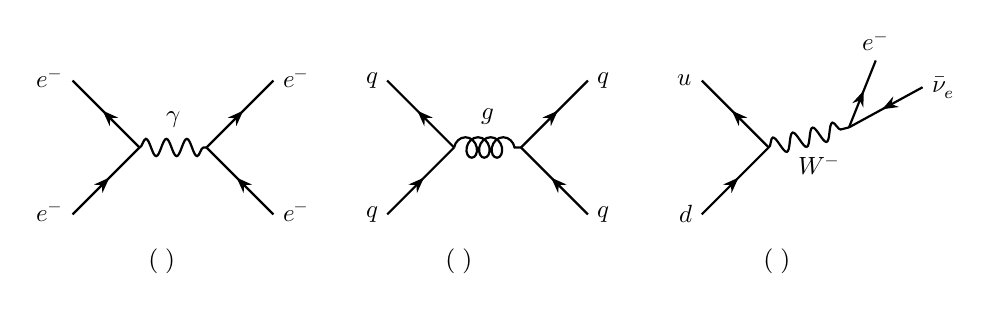
\begin{tikzpicture}[scale=0.85, photon/.style={decorate, decoration={snake, amplitude=1.1mm, segment length=2.6mm}, thick},
  gluon/.style={decorate, decoration={coil, amplitude=1.3mm, segment length=1.6mm, aspect=0.8}, thick},
  fermion/.style={thick, postaction={decorate}, decoration={markings, mark=at position 0.55 with {\arrow{Stealth[length=2mm]}}}}]
  % (a) e e рассеяние
  \begin{scope}
   \draw[fermion] (0,0) -- (1,1); \draw[fermion] (1,1) -- (0,2);
   \draw[fermion] (3,0) -- (2,1); \draw[fermion] (2,1) -- (3,2);
   \draw[photon] (1,1) -- (2,1);
   \node[left, font=\small] at (0,0) {$e^-$}; \node[left, font=\small] at (0,2) {$e^-$};
   \node[right, font=\small] at (3,0) {$e^-$}; \node[right, font=\small] at (3,2) {$e^-$};
   \node[above, font=\small] at (1.5,1.15) {$\gamma$};
   \node[font=\small] at (1.5,-0.7) {(а) ЭМ};
  \end{scope}
  % (b) q q рассеяние глюоном
  \begin{scope}[xshift=4.7cm]
   \draw[fermion] (0,0) -- (1,1); \draw[fermion] (1,1) -- (0,2);
   \draw[fermion] (3,0) -- (2,1); \draw[fermion] (2,1) -- (3,2);
   \draw[gluon] (1,1) -- (2,1);
   \node[left, font=\small] at (0,0) {$q$}; \node[left, font=\small] at (0,2) {$q$};
   \node[right, font=\small] at (3,0) {$q$}; \node[right, font=\small] at (3,2) {$q$};
   \node[above, font=\small] at (1.5,1.2) {$g$};
   \node[font=\small] at (1.5,-0.7) {(б) сильное};
  \end{scope}
  % (c) бета-распад нейтрона
  \begin{scope}[xshift=9.4cm]
   \draw[fermion] (0,0) -- (1,1); \draw[fermion] (1,1) -- (0,2);
   \draw[photon] (1,1) -- (2.2,1.3);
   \draw[fermion] (2.2,1.3) -- (2.6,2.3);
   \draw[fermion] (3.3,1.9) -- (2.2,1.3);
   \node[left, font=\small] at (0,0) {$d$}; \node[left, font=\small] at (0,2) {$u$};
   \node[above, font=\small] at (2.6,2.3) {$e^-$}; \node[right, font=\small] at (3.3,1.9) {$\bar\nu_e$};
   \node[below, font=\small] at (1.75,1.0) {$W^-$};
   \node[font=\small] at (1.5,-0.7) {(в) слабое};
  \end{scope}
\end{tikzpicture}
\caption{Диаграммы Фейнмана (время — снизу вверх): (а) рассеяние электронов обменом фотоном;
(б) рассеяние кварков обменом глюоном; (в) слабый распад $d\to u+e^-+\bar\nu_e$, лежащий в основе
бета-распада нейтрона (стрелка, направленная против времени, — античастица).}
\label{fig:14:feyn}
\end{figure}

\subsection{Фермионы: лептоны и кварки}

Фермионы со спином $\frac12$ образуют три поколения (семейства), одинаковые по зарядам и взаимодействиям,
но различающиеся массами.

\begin{table}[htbp]
\centering
\small
\caption{Фундаментальные фермионы Стандартной модели (массы — в единицах $c^{-2}$, приближённо).}
\label{tab:14:fermions}
\begin{tabular}{@{}lcccc@{}}
\toprule
& I поколение & II поколение & III поколение & Заряд $Q/e$ \\
\midrule
\multirow{2}{*}{Кварки}
 & $u$ — 2,2 МэВ & $c$ — 1,27 ГэВ & $t$ — 173 ГэВ & $+\tfrac23$ \\
 & $d$ — 4,7 МэВ & $s$ — 95 МэВ & $b$ — 4,18 ГэВ & $-\tfrac13$ \\
\midrule
\multirow{2}{*}{Лептоны}
 & $e^-$ — 0,511 МэВ & $\mu^-$ — 105,7 МэВ & $\tau^-$ — 1777 МэВ & $-1$ \\
 & $\nu_e$ & $\nu_\mu$ & $\nu_\tau$ & $0$ \\
\bottomrule
\end{tabular}
\end{table}

\paragraph{Лептоны} не участвуют в сильном взаимодействии. Заряженные лептоны $e,\mu,\tau$ участвуют в
электромагнитном и слабом взаимодействиях; $\mu$ и $\tau$ нестабильны ($\tau_\mu=2{,}2$~мкс, $\tau_\tau=2{,}9\cdot10^{-13}$~с).
Нейтрино — нейтральные, участвуют только в слабом взаимодействии; их массы ненулевые (доказано
наблюдением нейтринных осцилляций; Нобелевская премия 2015), но очень малы — меньше $\sim1$~эВ. Каждому
поколению приписывают лептонное число ($L_e$, $L_\mu$, $L_\tau$): $+1$ для лептона, $-1$ для антилептона.

\paragraph{Кварки} имеют дробный электрический заряд ($+\frac23e$ или $-\frac13e$), барионное число $\frac13$ и
дополнительное квантовое число — \emph{цвет} (три значения: «красный», «зелёный», «синий»). В свободном
состоянии не наблюдаются (конфайнмент): существуют только бесцветные комбинации — адроны (\tref{t:15}).
Шесть типов кварков называют \emph{ароматами}: $u,d,s,c,b,t$. Массы кварков указаны условно: лёгкие кварки
нельзя «взвесить» в свободном состоянии; их массы определяются косвенно.

\subsection{Переносчики взаимодействий}

\begin{itemize}
 \item \textbf{Фотон} $\gamma$: спин 1, масса 0, заряда нет. Взаимодействует с электрическим зарядом.
 \item \textbf{$W^\pm$, $Z^0$}: спин 1, массы $80{,}4$ и $91{,}2$~ГэВ; открыты в ЦЕРН в 1983~г. (К.~Руббиа, С.~ван~дер~Мер).
       $W^\pm$ меняют аромат фермиона (заряженные токи), $Z^0$ — нет (нейтральные токи, открыты в 1973~г.).
 \item \textbf{Глюоны} $g$: спин 1, масса 0, электрически нейтральны, но несут цвет (8 цветовых комбинаций);
       поэтому глюоны взаимодействуют друг с другом — это принципиальное отличие КХД от КЭД (\tref{t:15}).
\end{itemize}

\subsection{Бозон Хиггса}

Калибровочная симметрия требует, чтобы переносчики были безмассовыми, а слабые бозоны массивны.
Противоречие разрешается \emph{механизмом Хиггса} (Браут, Энглер, Хиггс, 1964): пространство заполнено
скалярным полем, имеющим ненулевое вакуумное среднее $v\approx246$~ГэВ. Взаимодействие с ним даёт массы:
\begin{itemize}
 \item $W^\pm$ и $Z^0$ — через спонтанное нарушение электрослабой симметрии ($M_W=\frac12gv$, $M_Z=M_W/\cos\theta_W$);
       фотон остаётся безмассовым;
 \item фермионам — через юкавские взаимодействия: $m_f=y_fv/\sqrt2$, поэтому константа связи фермиона с
       бозоном Хиггса пропорциональна его массе.
\end{itemize}
Квант этого поля — \emph{бозон Хиггса} $H$: спин 0, электрически нейтрален, масса $\approx125$~ГэВ. Открыт в
2012~г. на Большом адронном коллайдере (эксперименты ATLAS и CMS); Нобелевская премия 2013~г.
(Энглер, Хиггс). Он распадается преимущественно в пары $b\bar b$, а также $WW^*$, $\gamma\gamma$, $ZZ^*$ и др.
Механизм Хиггса не объясняет основную часть массы обычного вещества: масса протона ($938$~МэВ)
определяется энергией глюонного поля и движения кварков (КХД), а не массами $u$ и $d$ кварков ($\sim10$~МэВ в сумме).

\subsection{Законы сохранения}

\begin{center}
\small
\begin{tabular}{@{}lcccc@{}}
\toprule
Величина & Сильное & ЭМ & Слабое \\
\midrule
энергия, импульс, момент импульса, электрический заряд & да & да & да \\
барионное число $B$ & да & да & да \\
лептонные числа $L_e,L_\mu,L_\tau$ & да & да & да$^{*}$ \\
аромат (странность $S$, очарование, \dots) & да & да & нет \\
пространственная чётность $P$ & да & да & нет \\
\bottomrule
\end{tabular}

{\footnotesize $^{*}$ В процессах взаимодействия; нейтринные осцилляции нарушают сохранение отдельных $L_e,L_\mu,L_\tau$,
сохраняя полное $L$.}
\end{center}
Пример применения: распад $p\to e^++\gamma$ разрешён зарядом и энергией, но запрещён сохранением $B$ и $L$;
экспериментально $\tau_p>10^{34}$~лет.

\section{Математические выводы}

\begin{derivation}[label=der:14:yukawa]{радиус обменного взаимодействия}
\emph{Допущения:} оценка по порядку величины; покоящийся нуклон (или другая частица) испускает
виртуальный квант массы $M$.

В начальном состоянии энергия $E_0=m_Nc^2$. В промежуточном состоянии есть нуклон и квант с энергией
не менее $Mc^2$, т.\,е. закон сохранения энергии нарушен на $\Delta E\ge Mc^2$. Соотношение неопределённостей
$\Delta E\,\Delta t\sim\hbar$ разрешает такое состояние на время $\Delta t\sim\hbar/Mc^2$. Даже двигаясь со скоростью,
близкой к $c$, квант удаляется не более чем на
\[
  r_0\sim c\Delta t=\frac{\hbar}{Mc}.
\]
\emph{Размерность:} $[\hbar/Mc]=\text{эрг}\cdot\text{с}/(\text{г}\cdot\text{см}/\text{с})=\text{см}$.
\emph{Численно:} $\hbar c=197$~МэВ$\cdot$фм; для $\pi$-мезона ($139{,}6$~МэВ) $r_0=1{,}41$~фм — радиус ядерных
сил; для $W$ ($80\,400$~МэВ) — $2{,}5\cdot10^{-3}$~фм; для фотона ($M=0$) $r_0=\infty$.

\emph{Потенциал Юкавы.} Статическое поле массивного скалярного кванта удовлетворяет уравнению
$(\nabla^2-1/r_0^2)\phi=-4\pi g\delta(\vect r)$ (аналог уравнения Пуассона), решение которого
$\phi=g\,\ee^{-r/r_0}/r$. При $r_0\to\infty$ получаем кулоновский потенциал.
\end{derivation}

\begin{derivation}[label=der:14:compare]{сравнение интенсивностей взаимодействий}
\emph{Электромагнитное против гравитационного} для двух протонов:
\[
  \frac{F_{\text{эм}}}{F_{\text{гр}}}=\frac{e^2}{Gm_p^2}=\frac{(4{,}8\cdot10^{-10})^2}{6{,}67\cdot10^{-8}\cdot(1{,}67\cdot10^{-24})^2}\approx1{,}2\cdot10^{36}.
\]
Отношение не зависит от расстояния (обе силы $\propto1/r^2$). Гравитация в микромире пренебрежимо мала;
в макромире она доминирует, потому что тела электрически нейтральны, а «гравитационный заряд» (масса) всегда
положителен и складывается.

\emph{Слабое против электромагнитного.} Безразмерная мера слабого взаимодействия при энергии $E$:
$G_FE^2/(\hbar c)^3$. При $E\sim m_pc^2\approx1$~ГэВ это $\approx1{,}2\cdot10^{-5}$, тогда как $\alpha\approx7\cdot10^{-3}$. Константа
слабой связи $g$ сама по себе не мала ($g^2/4\pi\hbar c\approx1/30$); малость обусловлена множителем
$(E/M_Wc^2)^2$ — слабость «кажущаяся», связанная с массивностью переносчика:
$G_F/\sqrt2=g^2/8M_W^2$ (в системе $\hbar=c=1$).
\end{derivation}

\begin{derivation}[label=der:14:charges]{проверка зарядов в Стандартной модели}
Сумма электрических зарядов всех фермионов одного поколения с учётом трёх цветов кварков:
\[
  \underbrace{(-1)}_{e}+\underbrace{0}_{\nu}+3\Bigl(\underbrace{\tfrac23}_{u}+\underbrace{(-\tfrac13)}_{d}\Bigr)=-1+3\cdot\tfrac13=0 .
\]
Это условие сокращения аномалий, необходимое для внутренней согласованности (перенормируемости) теории;
оно связывает число цветов с дробностью зарядов кварков и указывает на глубокую связь лептонов и кварков.
\end{derivation}

\section{Итоговые формулы}

\keyformula{r_0\sim\frac{\hbar}{Mc},\qquad U(r)\propto-\frac{g^2}{r}\ee^{-r/r_0}}
 {$M$ — масса переносчика, $g$ — константа связи, $r_0$ — радиус действия.}
 {оценка по порядку величины; статический предел.}
 {радиус взаимодействия по массе переносчика и наоборот (пион, $W$).}

\keyformula{\alpha=\frac{e^2}{\hbar c}\approx\frac{1}{137},\quad \alpha_s\sim1\ (\text{при}\sim1\ \text{ГэВ}),\quad \frac{G_F}{(\hbar c)^3}=1{,}166\cdot10^{-5}\ \text{ГэВ}^{-2}}
 {$\alpha$, $\alpha_s$ — константы электромагнитной и сильной связи; $G_F$ — постоянная Ферми.}
 {значения зависят от энергии (бегущие константы).}
 {сравнение интенсивностей взаимодействий и времён процессов.}

\keyformula{m_f=\frac{y_fv}{\sqrt2},\quad M_W=\frac{gv}{2},\quad M_Z=\frac{M_W}{\cos\theta_W},\quad v\approx246\ \text{ГэВ}}
 {$y_f$ — юкавская константа фермиона, $g$ — константа $SU(2)$, $\theta_W$ — угол Вайнберга ($\sin^2\theta_W\approx0{,}23$).}
 {Стандартная модель, $\hbar=c=1$ (для справки).}
 {происхождение масс $W$, $Z$ и фермионов.}

\section{Физическая интерпретация}

\textbf{Структура.} Вещество состоит из фермионов первого поколения ($u$, $d$, $e$); второе и третье поколения
нестабильны и рождаются в столкновениях высоких энергий. Число поколений с лёгкими нейтрино равно трём — это
установлено по ширине распада $Z^0$ (LEP, 1989--2000): $N_\nu=2{,}98\pm0{,}01$.

\textbf{Масса и радиус.} Связь $r_0=\hbar/Mc$ объясняет, почему дальнодействующие силы (электромагнитная,
гравитационная) имеют безмассовых переносчиков. Сильное взаимодействие короткодействующее по другой причине:
глюоны безмассовы, но из-за конфайнмента цветные объекты не распространяются дальше $\sim1$~фм.

\textbf{Экспериментальный статус.} Предсказания СМ подтверждены с высокой точностью (аномальный магнитный момент
электрона, свойства $W$ и $Z$, сечения процессов КХД). За её пределами остаются гравитация, тёмная материя и
тёмная энергия, массы нейтрино и преобладание вещества над антивеществом.

\section{Что необходимо знать на экзамене}

\begin{examcheck}
\checkhead{Определения}
\begin{itemize}
 \item фундаментальная частица; лептоны, кварки (ароматы, цвет), поколения; переносчики; античастицы;
 \item четыре взаимодействия: кто участвует, переносчики, радиусы, относительная сила.
\end{itemize}
\checkhead{Формулы и числа}
\begin{itemize}
 \item $r_0\sim\hbar/Mc$; потенциал Юкавы; $\hbar c=197$~МэВ$\cdot$фм;
 \item $\alpha\approx1/137$, $\alpha_s\sim1$, $G_F$; $M_W\approx80$~ГэВ, $M_Z\approx91$~ГэВ, $M_H\approx125$~ГэВ;
 \item заряды кварков $+\frac23$, $-\frac13$; массы $e,\mu,\tau$.
\end{itemize}
\checkhead{Выводы}
\begin{itemize}
 \item оценка радиуса обменного взаимодействия (пион, $W$-бозон);
 \item сравнение гравитационного и электромагнитного взаимодействий; «кажущаяся» слабость слабого взаимодействия.
\end{itemize}
\checkhead{Интерпретации}
\begin{itemize}
 \item роль бозона Хиггса (массы $W$, $Z$, фермионов) и почему масса протона — не от Хиггса;
 \item законы сохранения ($B$, $L$, аромат, чётность) и их нарушение слабым взаимодействием; ограничения СМ.
\end{itemize}
\end{examcheck}

% ======================================================================
\chapter[Кварковая структура адронов. Квантовая хромодинамика]%
        {Кварковая структура адронов. Сильное взаимодействие и КХД}
\label{t:15}
% ======================================================================

\begin{qbox}
\textbf{Билет 15.} Кварковая структура адронов — мезоны, барионы. Сильное взаимодействие,
квантовая хромодинамика.
\end{qbox}

\section{Содержание билета}

\textbf{Подтемы:}
\begin{enumerate}
 \item адроны; кварковая модель: мезоны ($q\bar q$) и барионы ($qqq$); квантовые числа и их проверка;
 \item цвет: проблема $\Delta^{++}$ и $\Omega^-$, бесцветность адронов, экспериментальная проверка числа цветов (отношение $R$);
 \item экспериментальные свидетельства кварков: глубоконеупругое рассеяние, струи;
 \item квантовая хромодинамика: глюоны, самодействие, асимптотическая свобода, конфайнмент, потенциал кварк--антикварк;
 \item сильное взаимодействие нуклонов как «остаточное» цветовое; происхождение масс адронов.
\end{enumerate}

\textbf{Необходимые понятия:} Стандартная модель, кварки и переносчики (\tref{t:14}); принцип Паули
(\tref{t:13}); законы сохранения зарядов; спин и сложение моментов.

\section{Определения и физические принципы}

\begin{definition}[адроны]
\emph{Адроны} — частицы, участвующие в сильном взаимодействии. Делятся на \emph{мезоны} (целый спин,
барионное число $B=0$) и \emph{барионы} (полуцелый спин, $B=1$; антибарионы — $B=-1$). Лёгчайшие барионы —
нуклоны (протон и нейтрон), лёгчайшие мезоны — $\pi$-мезоны.
\end{definition}

\begin{principle}{Кварковая модель (Гелл-Ман, Цвейг, 1964)}
Мезоны — связанные состояния кварка и антикварка ($q\bar q'$), барионы — трёх кварков ($qqq$).
Кварки имеют спин $\frac12$, барионное число $\frac13$, электрический заряд $+\frac23e$ ($u,c,t$) или $-\frac13e$ ($d,s,b$).
Квантовые числа адрона — суммы квантовых чисел составляющих (с учётом орбитального движения для спина и чётности).
\end{principle}

\begin{definition}[цвет и квантовая хромодинамика]
\emph{Цвет} — квантовое число кварков, принимающее три значения ($r,g,b$); антикварки несут антицвета.
\emph{Квантовая хромодинамика} (КХД) — калибровочная теория сильного взаимодействия с группой $SU(3)$:
кварки взаимодействуют обменом восемью безмассовыми глюонами, которые сами несут цвет.
Наблюдаемые адроны — цветовые синглеты («бесцветны»).
\end{definition}

\emph{Физический смысл.} Сильное взаимодействие нуклонов в ядре (\tref{t:17}) — не фундаментальное, а
«остаточное» проявление цветового взаимодействия кварков, подобно ван-дер-ваальсовым силам между
нейтральными атомами как остатку электромагнитных сил.

\emph{Область применимости.} Кварковая модель с «составляющими» кварками качественно описывает спектр и
квантовые числа адронов. Теория возмущений КХД применима лишь при больших передачах импульса
($Q\gg1$~ГэВ), где $\alpha_s\ll1$; явления на масштабе $\sim1$~фм (массы адронов, конфайнмент) требуют
непертурбативных методов (решёточная КХД).

\section{Основная теория}

\subsection{Проблема: систематика адронов}

К началу 1960-х годов было известно множество адронов. Группировка частиц с одинаковыми спином и чётностью
в координатах «проекция изоспина -- странность» дала правильные фигуры — октеты и декуплет («восьмеричный
путь», Гелл-Ман, Нееман, 1961). Такие мультиплеты естественно возникают, если адроны составлены из трёх
лёгких кварков $u,d,s$ (\emph{странность} $S=-1$ для $s$-кварка, $+1$ для $\bar s$). Предсказание по декуплету
бариона $\Omega^-$ (масса $\approx1680$~МэВ, $S=-3$) и его открытие в 1964~г. (масса 1672~МэВ) стало триумфом
модели.

\subsection{Мезоны}

Мезон $q\bar q'$: $B=\frac13-\frac13=0$; спины кварков $\frac12\otimes\frac12$ дают $S=0$ или $1$; при нулевом
орбитальном моменте — псевдоскалярные ($J=0$) и векторные ($J=1$) мезоны.
\begin{center}
\small
\begin{tabular}{@{}lllll@{}}
\toprule
Мезон & Состав & $Q/e$ & $J$ & Масса, МэВ \\
\midrule
$\pi^+$, $\pi^-$ & $u\bar d$, $d\bar u$ & $+1$, $-1$ & 0 & 139,6 \\
$\pi^0$ & $(u\bar u-d\bar d)/\sqrt2$ & 0 & 0 & 135,0 \\
$K^+$, $K^0$ & $u\bar s$, $d\bar s$ & $+1$, 0 & 0 & 493,7; 497,6 \\
$\rho^+$ & $u\bar d$ & $+1$ & 1 & 775 \\
$J/\psi$ & $c\bar c$ & 0 & 1 & 3097 \\
$\Upsilon$ & $b\bar b$ & 0 & 1 & 9460 \\
\bottomrule
\end{tabular}
\end{center}
Открытие узкого резонанса $J/\psi$ в 1974~г. («ноябрьская революция») доказало существование $c$-кварка;
$\Upsilon$ (1977) — $b$-кварка; $t$-кварк открыт в 1995~г. на Тэватроне (он распадается раньше, чем успевает
образовать адрон).

\subsection{Барионы}

Барион $qqq$: $B=1$; спины трёх кварков дают $J=\frac12$ или $\frac32$ (при нулевых орбитальных моментах).
\begin{center}
\small
\begin{tabular}{@{}lllll@{}}
\toprule
Барион & Состав & $Q/e$ & $J$ & Масса, МэВ \\
\midrule
$p$ & $uud$ & $+1$ & $\frac12$ & 938,3 \\
$n$ & $udd$ & 0 & $\frac12$ & 939,6 \\
$\Lambda^0$ & $uds$ & 0 & $\frac12$ & 1116 \\
$\Sigma^+$ & $uus$ & $+1$ & $\frac12$ & 1189 \\
$\Delta^{++}$ & $uuu$ & $+2$ & $\frac32$ & 1232 \\
$\Omega^-$ & $sss$ & $-1$ & $\frac32$ & 1672 \\
\bottomrule
\end{tabular}
\end{center}
Проверка зарядов (вывод~\ref{der:15:charges}): $p$: $\frac23+\frac23-\frac13=1$; $n$: $\frac23-\frac13-\frac13=0$;
$\Delta^{++}$: $3\cdot\frac23=2$; $\Omega^-$: $3\cdot(-\frac13)=-1$. Нет адронов с дробным зарядом и нет
адронов из двух кварков — модель объясняет, почему.

\begin{figure}[htbp]
\centering
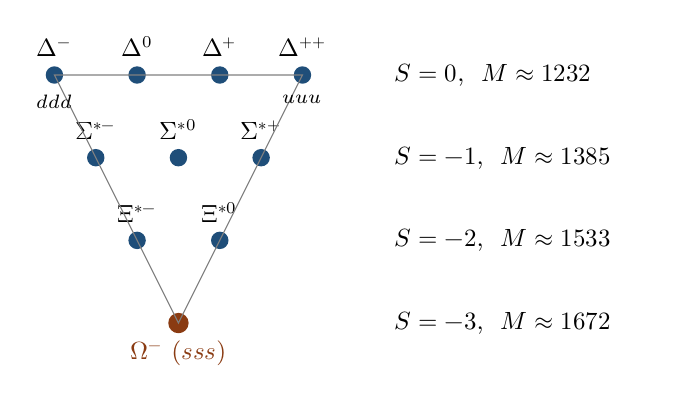
\begin{tikzpicture}[scale=1.05]
  \foreach \x/\lab in {0/{$\Delta^-$},1/{$\Delta^0$},2/{$\Delta^+$},3/{$\Delta^{++}$}} { \fill[accent] (\x,0) circle (3pt); \node[above, font=\small] at (\x,0.1) {\lab}; }
  \foreach \x/\lab in {0.5/{$\Sigma^{*-}$},1.5/{$\Sigma^{*0}$},2.5/{$\Sigma^{*+}$}} { \fill[accent] (\x,-1) circle (3pt); \node[above, font=\small] at (\x,-0.9) {\lab}; }
  \foreach \x/\lab in {1/{$\Xi^{*-}$},2/{$\Xi^{*0}$}} { \fill[accent] (\x,-2) circle (3pt); \node[above, font=\small] at (\x,-1.9) {\lab}; }
  \fill[keycol] (1.5,-3) circle (3.5pt); \node[below, font=\small, keycol] at (1.5,-3.1) {$\Omega^-$ ($sss$)};
  \draw[gray] (0,0) -- (3,0) -- (1.5,-3) -- cycle;
  \foreach \y/\S/\m in {0/0/1232,-1/{-1}/1385,-2/{-2}/1533,-3/{-3}/1672} {
     \node[font=\small, anchor=west] at (4.0,\y) {$S=\S$, \ $M\approx\m$~МэВ};
  }
  \node[font=\scriptsize, below] at (0,-0.12) {$ddd$};
  \node[font=\scriptsize, below] at (3,-0.12) {$uuu$};
\end{tikzpicture}
\caption{Барионный декуплет $J=\frac32$. Каждый шаг вниз — замена $u$ или $d$ кварка на $s$ и увеличение массы
примерно на 150~МэВ; эквидистантность позволила предсказать массу $\Omega^-$.}
\label{fig:15:decuplet}
\end{figure}

\subsection{Цвет}

\paragraph{Проблема.} $\Delta^{++}=uuu$ со спином $\frac32$ и $L=0$: пространственная функция симметрична (основное
состояние), спиновая — тоже (все три спина параллельны), ароматная — тоже (три $u$). Полная функция трёх
тождественных фермионов оказывается симметричной — противоречие с принципом Паули. То же для $\Omega^-=sss$.

\paragraph{Решение} (Боголюбов, Струминский, Тавхелидзе; Хан, Намбу, 1965): кварки несут дополнительное
квантовое число с тремя значениями — цвет; волновая функция бариона антисимметрична по цвету:
\[
  \Psi_{\text{цвет}}=\frac{1}{\sqrt6}\sum_{ijk}\varepsilon_{ijk}\,q_iq_jq_k ,
\]
и полная функция (пространство $\times$ спин $\times$ аромат $\times$ цвет) становится антисимметричной. Мезон —
$\frac{1}{\sqrt3}(r\bar r+g\bar g+b\bar b)$. Обе комбинации инвариантны относительно цветовых преобразований
(цветовые синглеты). \emph{Гипотеза конфайнмента}: в природе наблюдаются только бесцветные состояния. Это
объясняет, почему существуют $q\bar q$ и $qqq$ (а также экзотические тетра- и пентакварки, обнаруженные в 2000--2010-х годах), но
не $qq$ или одиночные кварки.

\paragraph{Экспериментальная проверка числа цветов.} Отношение сечений (вывод~\ref{der:15:R})
\begin{equation}\label{eq:15:R}
  R=\frac{\sigma(e^+e^-\to\text{адроны})}{\sigma(e^+e^-\to\mu^+\mu^-)}=N_c\sum_qQ_q^2
\end{equation}
при энергиях, где рождаются $u,d,s$, равно $N_c\cdot\frac23$, выше порога $c\bar c$ — $N_c\cdot\frac{10}{9}$, выше $b\bar b$ —
$N_c\cdot\frac{11}{9}$. Измерения дают $R\approx2$, $\frac{10}{3}$, $\frac{11}{3}$ (с небольшой поправкой КХД $1+\alpha_s/\pi$), т.\,е.
$N_c=3$. Число цветов подтверждается также шириной распада $\pi^0\to2\gamma$ (амплитуда $\propto N_c$).

\subsection{Экспериментальные свидетельства кварков}

\begin{enumerate}
 \item \textbf{Глубоконеупругое рассеяние электронов на протонах} (SLAC, 1968; Нобелевская премия 1990): при больших
       передачах импульса сечение ведёт себя как при рассеянии на \emph{точечных} частицах со спином $\frac12$
       («партонах») — аналог опыта Резерфорда для протона. Выяснилось также, что кварки несут лишь около
       половины импульса протона; остальное — глюоны.
 \item \textbf{Адронные струи.} В $e^+e^-$-аннигиляции рождённые кварк и антикварк превращаются в два узких пучка адронов
       (струи), угловое распределение которых соответствует спину $\frac12$. Трёхструйные события (DESY, 1979) —
       испускание жёсткого глюона: прямое наблюдение глюона.
 \item \textbf{Спектроскопия} кваркония ($c\bar c$, $b\bar b$) — система уровней, подобная позитронию, хорошо описываемая
       потенциалом~\eqref{eq:15:V}.
\end{enumerate}

\subsection{Квантовая хромодинамика}

\paragraph{Глюоны.} Кварк при испускании глюона может менять цвет ($r\to g$), поэтому глюон несёт пару «цвет--антицвет»;
из $3\times3=9$ комбинаций одна (синглет $(r\bar r+g\bar g+b\bar b)/\sqrt3$) не меняет цвета и не входит в теорию, остаётся
$8$ глюонов. Глюоны цветные и взаимодействуют друг с другом (вершины $ggg$ и $gggg$) — в этом главное отличие
от фотона, который не заряжен.

\paragraph{Асимптотическая свобода.} Эффективная константа связи зависит от передаваемого импульса $Q$
(«бегущая константа»). В КЭД заряд экранируется виртуальными парами, и $\alpha$ медленно растёт с энергией. В КХД
самодействие глюонов приводит к \emph{антиэкранировке}, и $\alpha_s$ убывает (Гросс, Вильчек, Политцер, 1973;
Нобелевская премия 2004). В однопетлевом приближении (без вывода)
\begin{equation}\label{eq:15:alphas}
  \alpha_s(Q^2)=\frac{12\pi}{(33-2n_f)\ln(Q^2/\Lambda^2)},
\end{equation}
где $n_f$ — число активных ароматов, $\Lambda\approx0{,}2$--$0{,}3$~ГэВ. Значения: $\alpha_s(M_Zc)\approx0{,}118$, при $Q\sim1$~ГэВ
$\alpha_s\sim0{,}5$. На малых расстояниях кварки почти свободны (что и видно в глубоконеупругом рассеянии), на расстояниях
$\sim\hbar/\Lambda\sim1$~фм взаимодействие становится сильным.

\paragraph{Конфайнмент.} Феноменологический потенциал кварк--антикварк:
\begin{equation}\label{eq:15:V}
  V(r)=-\frac43\frac{\alpha_s\hbar c}{r}+\kappa r,\qquad \kappa\approx0{,}9\text{--}1\ \text{ГэВ/фм}.
\end{equation}
На малых $r$ — кулоноподобное притяжение (обмен одним глюоном; множитель $\frac43$ — цветовой), на больших —
линейно растущий потенциал: силовые линии глюонного поля собираются в узкую «трубку» (струну) с постоянной
энергией на единицу длины, и сила $\approx\kappa\approx16$~т не убывает с расстоянием. При растяжении струны на
$\sim1$--$1{,}5$~фм её энергия становится достаточной для рождения пары $q\bar q$, струна рвётся, и образуются два
бесцветных адрона — изолированный кварк не появляется (рис.~\ref{fig:15:V}). Этот процесс (адронизация) порождает струи.

\begin{figure}[htbp]
\centering
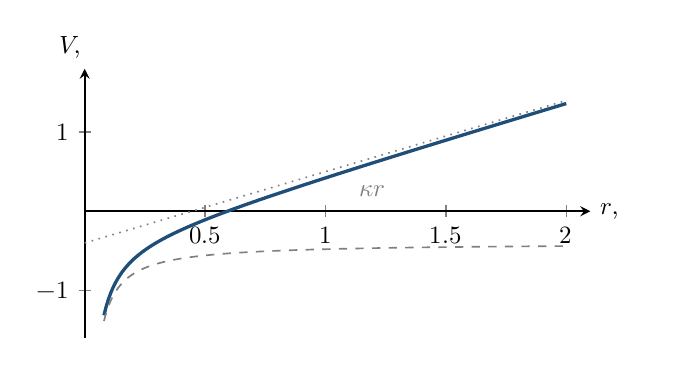
\begin{tikzpicture}
\begin{axis}[width=0.66\linewidth, height=5.0cm, axis lines=middle, xlabel={$r$, фм}, ylabel={$V$, ГэВ},
   xmin=0, xmax=2.1, ymin=-1.6, ymax=1.8, samples=200,
   xlabel style={at={(ticklabel* cs:1)}, anchor=west}, ylabel style={at={(ticklabel* cs:1)}, anchor=south}]
  \addplot[very thick, accent, domain=0.08:2.0] {-4/3*0.3*0.1973/x + 0.9*x - 0.4};
  \addplot[gray, dashed, domain=0.08:2.0] {-4/3*0.3*0.1973/x - 0.4};
  \addplot[gray, dotted, domain=0:2.0] {0.9*x-0.4};
  \node[font=\small, gray, anchor=west] at (axis cs:1.15,-0.85) {кулоновская часть};
  \node[font=\small, gray, anchor=west] at (axis cs:1.1,0.25) {$\kappa r$};
\end{axis}
\end{tikzpicture}
\caption{Потенциал кварк--антикварк~\eqref{eq:15:V} при $\alpha_s=0{,}3$, $\kappa=0{,}9$~ГэВ/фм (начало отсчёта энергии
выбрано произвольно). На больших расстояниях энергия растёт линейно — конфайнмент.}
\label{fig:15:V}
\end{figure}

\paragraph{Происхождение масс адронов.} Суммарная масса токовых кварков протона $2m_u+m_d\approx9$~МэВ — около 1\,\% его массы.
Остальное — энергия глюонного поля и кинетическая энергия кварков, локализованных в области $\sim1$~фм
($p\sim\hbar/R\sim200$--$300$~МэВ$/c$). В модели составляющих кварков им приписывают «эффективные» массы $\sim300$~МэВ
($u,d$) и $\sim500$~МэВ ($s$); это объясняет, например, $M_\Lambda-M_p\approx180$~МэВ.

\paragraph{Ядерные силы.} Нуклоны бесцветны, поэтому между ними действуют лишь остаточные силы на расстояниях, где
их кварковые облака перекрываются. На расстояниях $\sim1$--$2$~фм притяжение эффективно описывается обменом пионами
(лёгчайшими $q\bar q$ состояниями), радиус $\hbar/m_\pi c\approx1{,}4$~фм (\tref{t:14}).

\section{Математические выводы}

\begin{derivation}[label=der:15:charges]{квантовые числа адронов из кварков}
Используем аддитивность: $Q=\sum Q_q$, $B=\sum B_q$ ($B_q=\frac13$, $B_{\bar q}=-\frac13$), $S=-(N_s-N_{\bar s})$.

$\pi^+=u\bar d$: $Q=\frac23+\frac13=1$, $B=0$, $S=0$. \quad $K^+=u\bar s$: $Q=\frac23+\frac13=1$, $S=+1$.

$\Lambda=uds$: $Q=\frac23-\frac13-\frac13=0$, $B=1$, $S=-1$. \quad $\Omega^-=sss$: $Q=-1$, $B=1$, $S=-3$.

\emph{Спины.} Сложение трёх спинов $\frac12$: $\frac12\otimes\frac12\otimes\frac12=\frac32\oplus\frac12\oplus\frac12$; при $L=0$ барионы имеют
$J=\frac12$ (октет) или $\frac32$ (декуплет). Два спина: $\frac12\otimes\frac12=1\oplus0$ — мезоны $J=0$ и $1$.

\emph{Почему $\Delta^{++}$ требует цвета:} спин $\frac32$ означает $m_s=+\frac12$ у всех трёх кварков (в состоянии $J_z=\frac32$),
ароматы одинаковы, $L=0$ — функция без цвета симметрична по всем перестановкам, что запрещено для фермионов.
\end{derivation}

\begin{derivation}[label=der:15:R]{отношение $R$ и число цветов}
\emph{Допущения:} энергия $\sqrt s$ много больше масс рождающихся кварков, но ниже порога $Z^0$; аннигиляция идёт через
виртуальный фотон; поправки КХД отброшены.

Сечение $e^+e^-\to\gamma^*\to f\bar f$ для точечного фермиона с зарядом $Q_fe$ пропорционально квадрату заряда
(амплитуда $\propto eQ_fe$): $\sigma(f\bar f)=Q_f^2\,\sigma(\mu^+\mu^-)$, $\sigma(\mu^+\mu^-)=\dfrac{4\pi\alpha^2(\hbar c)^2}{3s}$.
Кварк каждого аромата рождается в $N_c$ цветовых вариантах, а адронизация происходит с вероятностью 1:
\[
  R=\frac{\sum_q N_c\,Q_q^2\,\sigma(\mu\mu)}{\sigma(\mu\mu)}=N_c\sum_qQ_q^2 .
\]
Для $u,d,s$: $\sum Q^2=\frac49+\frac19+\frac19=\frac23$; с $c$: $+\frac49=\frac{10}9$; с $b$: $+\frac19=\frac{11}9$. При $N_c=3$:
$R=2$; $\frac{10}{3}\approx3{,}3$; $\frac{11}{3}\approx3{,}7$, что согласуется с опытом. При $N_c=1$ было бы $R=\frac23$, $\frac{10}9$, $\frac{11}9$ —
втрое меньше наблюдаемого.
\end{derivation}

\begin{derivation}[label=der:15:string]{оценка расстояния разрыва струны}
Энергия струны длины $r$ равна $\kappa r$. Рождение лёгкой пары $q\bar q$ (с образованием двух мезонов) энергетически
выгодно, когда $\kappa r\gtrsim2m_{\text{эфф}}c^2$, где $m_{\text{эфф}}c^2\sim0{,}3$--$0{,}5$~ГэВ (масса составляющего кварка или
порядок массы лёгкого адрона). Отсюда $r\gtrsim2\cdot(0{,}3\text{--}0{,}5)/0{,}9$~фм $\approx0{,}7$--$1{,}1$~фм — масштаб размеров адронов.
Сила натяжения: $\kappa=1\ \text{ГэВ/фм}=1{,}6\cdot10^{-10}\ \text{Дж}/10^{-15}\ \text{м}=1{,}6\cdot10^{5}$~Н $\approx16$~тонн-силы.
\end{derivation}

\begin{derivation}[label=der:15:af]{масштаб $\Lambda$ и размер адронов}
По~\eqref{eq:15:alphas} $\alpha_s\to\infty$ при $Q\to\Lambda$: теория возмущений перестаёт работать на масштабе импульсов
$\sim\Lambda\approx0{,}2$--$0{,}3$~ГэВ$/c$, т.\,е. на расстояниях $r\sim\hbar/\Lambda=\hbar c/(\Lambda c)\approx197/250\ \text{фм}\approx0{,}8$~фм. Это
естественный размер адронов: КХД содержит размерный масштаб, возникающий из безразмерной константы
благодаря её «бегу» (размерная трансмутация).
\end{derivation}

\section{Итоговые формулы}

\keyformula{\text{мезон}=q\bar q',\quad \text{барион}=qqq,\quad Q_u=+\tfrac23,\ Q_d=Q_s=-\tfrac13,\quad B_q=\tfrac13}
 {$Q$ — заряд в единицах $e$, $B$ — барионное число.}
 {кварковая модель; квантовые числа аддитивны.}
 {состав и квантовые числа адронов; проверка законов сохранения в реакциях.}

\keyformula{R=\frac{\sigma(e^+e^-\to\text{адроны})}{\sigma(e^+e^-\to\mu^+\mu^-)}=N_c\sum_qQ_q^2}
 {$N_c$ — число цветов, сумма по ароматам, рождение которых энергетически доступно.}
 {энергии много выше порогов кварков и ниже $M_Z$; низший порядок по $\alpha_s$.}
 {экспериментальное определение $N_c=3$ и зарядов кварков.}

\keyformula{\alpha_s(Q^2)=\frac{12\pi}{(33-2n_f)\ln(Q^2/\Lambda^2)},\qquad V(r)=-\frac43\frac{\alpha_s\hbar c}{r}+\kappa r}
 {$n_f$ — число активных ароматов, $\Lambda\approx0{,}2$--$0{,}3$~ГэВ, $\kappa\approx1$~ГэВ/фм.}
 {первая формула — однопетлевое приближение при $Q\gg\Lambda$; вторая — феноменологическая.}
 {асимптотическая свобода и конфайнмент; спектры кваркония.}

\section{Физическая интерпретация}

\textbf{Два режима одного взаимодействия.} На малых расстояниях ($\ll1$~фм) кварки ведут себя почти как свободные
(асимптотическая свобода — партонная картина глубоконеупругого рассеяния), на больших — притяжение растёт
(конфайнмент). Поэтому кварки «видны» в столкновениях высоких энергий, но никогда не вылетают поодиночке.

\textbf{Сравнение с КЭД.} Структура теорий подобна (калибровочные бозоны со спином 1), но цветной заряд глюонов
меняет знак «бега» константы. В КЭД нет конфайнмента: электрон и позитрон можно разделить.

\textbf{Иерархия масштабов.} Сильные распады ($\Delta\to N\pi$) идут за $\sim10^{-23}$~с ($\Gamma\approx120$~МэВ). Слабые распады
странных частиц ($\Lambda\to p\pi^-$) — за $\sim10^{-10}$~с, потому что сильное взаимодействие сохраняет странность, а
изменить аромат может лишь слабое (\tref{t:16}).

\section{Что необходимо знать на экзамене}

\begin{examcheck}
\checkhead{Определения}
\begin{itemize}
 \item адроны, мезоны, барионы; кварковый состав $p,n,\pi^\pm,\pi^0,K^+,\Lambda,\Delta^{++},\Omega^-$;
 \item цвет, цветовой синглет, конфайнмент, асимптотическая свобода, глюоны (8, цветные).
\end{itemize}
\checkhead{Формулы}
\begin{itemize}
 \item заряды и барионные числа кварков; $R=N_c\sum Q_q^2$;
 \item $V(r)=-\frac43\alpha_s\hbar c/r+\kappa r$; качественный вид $\alpha_s(Q^2)$ (убывает логарифмически).
\end{itemize}
\checkhead{Выводы}
\begin{itemize}
 \item проверка зарядов и спинов адронов; проблема $\Delta^{++}$ и её решение цветом;
 \item вычисление $R$ для $u,d,s$ / $+c$ / $+b$ и вывод $N_c=3$.
\end{itemize}
\checkhead{Интерпретации}
\begin{itemize}
 \item эксперименты: глубоконеупругое рассеяние, струи, $J/\psi$; предсказание $\Omega^-$;
 \item почему одиночные кварки не наблюдаются (разрыв струны); откуда масса протона; ядерные силы как остаточные.
\end{itemize}
\end{examcheck}

% ======================================================================
\chapter[Слабое взаимодействие. \texorpdfstring{$W^\pm$, $Z^0$}{W±, Z0} бозоны. Слабые распады]%
        {Слабое взаимодействие. \texorpdfstring{$W^\pm$, $Z^0$}{W±, Z0} бозоны. Слабые распады}
\label{t:16}
% ======================================================================

\begin{qbox}
\textbf{Билет 16.} Слабое взаимодействие. $W^\pm$, $Z^0$ бозоны, слабые распады лептонов и адронов.
\end{qbox}

\section{Содержание билета}

\textbf{Подтемы:}
\begin{enumerate}
 \item общие свойства слабого взаимодействия: универсальность, малый радиус, изменение аромата, нарушение чётности;
 \item переносчики $W^\pm$ и $Z^0$: заряженные и нейтральные токи, массы, открытие; теория Ферми и её связь с массой $W$;
 \item электрослабое объединение (качественно);
 \item слабые распады лептонов: распад мюона и $\tau$-лептона, закон Сарджента;
 \item слабые распады адронов: $\beta$-распад нейтрона, распады $\pi$, $K$, $\Lambda$; угол Кабиббо;
 \item законы сохранения и их нарушения в слабых процессах.
\end{enumerate}

\textbf{Необходимые понятия:} Стандартная модель и обменный механизм (\tref{t:14}); кварковый состав
адронов (\tref{t:15}); спиральность; время жизни и ширина (\tref{t:02}).

\section{Определения и физические принципы}

\begin{definition}[слабое взаимодействие]
Фундаментальное взаимодействие, в котором участвуют все лептоны и кварки; единственное, способное
изменять аромат фермионов ($d\to u$, $\mu\to\nu_\mu$, $s\to u$). Переносчики — массивные векторные бозоны $W^+$, $W^-$
($M_W=80{,}4$~ГэВ) и $Z^0$ ($M_Z=91{,}2$~ГэВ).
\end{definition}

\begin{definition}[заряженные и нейтральные токи]
\emph{Заряженный ток} — процесс с обменом $W^\pm$: заряд лептона или кварка меняется на единицу ($e^-\leftrightarrow\nu_e$,
$d\leftrightarrow u$). \emph{Нейтральный ток} — обмен $Z^0$: фермион остаётся тем же ($\nu_\mu e^-\to\nu_\mu e^-$).
Нейтральные токи с изменением аромата (например, $s\to d$ через $Z^0$) в низшем порядке отсутствуют.
\end{definition}

\begin{definition}[спиральность]
Проекция спина на направление импульса, $h=\vect s\cdot\vect p/|\vect p|$ (в единицах $\hbar$). Левая спиральность — $h=-\frac12$.
В заряженных токах участвуют только левые (по киральности) фермионы и правые антифермионы; для безмассовых
частиц это совпадает со спиральностью: нейтрино левые, антинейтрино правые.
\end{definition}

\emph{Физический смысл.} Слабое взаимодействие отвечает за процессы, недоступные сильному и
электромагнитному: бета-распад, распады мюона, пионов, странных частиц, термоядерный $pp$-цикл на Солнце
($p+p\to d+e^++\nu_e$), рассеяние нейтрино.

\emph{Область применимости описания.} При энергиях $E\ll M_Wc^2$ взаимодействие эффективно точечное (теория
Ферми с константой $G_F$). При $E\sim M_Wc^2$ необходимо явное описание обмена $W$, $Z$ в рамках электрослабой теории.

\section{Основная теория}

\subsection{Проблема и история}

Бета-распад с непрерывным спектром электронов привёл к гипотезе нейтрино (Паули, 1930) и к первой теории
слабого взаимодействия (Ферми, 1934): четыре фермиона взаимодействуют в одной точке с константой
$G_F$. Теория описывала распады, но предсказывала неограниченный рост сечений с энергией ($\sigma\propto G_F^2E^2$),
что недопустимо физически (нарушение унитарности при $E\sim300$~ГэВ). Решение — переносчик конечной массы:
при $E\ll Mc^2$ взаимодействие выглядит точечным, а при больших энергиях рост сечений прекращается.

\subsection{Свойства слабого взаимодействия}

\begin{enumerate}
 \item \textbf{Малый радиус:} $r_W=\hbar/M_Wc\approx2{,}5\cdot10^{-3}$~фм (\tref{t:14}).
 \item \textbf{«Слабость» при низких энергиях:} амплитуда обмена $W$ пропорциональна $g^2/(q^2-M_W^2c^2)$; при
       $q^2\ll M_W^2c^2$ это константа $\propto g^2/M_W^2$, т.\,е. точечное взаимодействие с
       \begin{equation}\label{eq:16:GF}
         \frac{G_F}{\sqrt2}=\frac{g^2}{8M_W^2}\quad(\hbar=c=1),\qquad \frac{G_F}{(\hbar c)^3}=1{,}166\cdot10^{-5}\ \text{ГэВ}^{-2}.
       \end{equation}
       Сама константа $g$ сравнима с электрическим зарядом ($e=g\sin\theta_W$, $\sin^2\theta_W\approx0{,}23$).
 \item \textbf{Универсальность:} лептоны и кварки (с учётом смешивания) взаимодействуют с $W$ с одной константой.
 \item \textbf{Изменение аромата} — только через $W^\pm$; поэтому лёгчайшие частицы каждого аромата
       ($\mu$, $\pi^\pm$, $K$, $\Lambda$, нейтрон) распадаются только слабо и живут долго.
 \item \textbf{Нарушение чётности ($P$) и зарядового сопряжения ($C$)}, слабое нарушение $CP$.
\end{enumerate}

\paragraph{Нарушение чётности.} Т.~Ли и Ч.~Янг (1956) указали, что сохранение чётности в слабых процессах не
проверено. В опыте Ц.~Ву (1957) ядра $^{60}$Co поляризовались магнитным полем при $T\approx0{,}01$~К; электроны
бета-распада вылетали преимущественно \emph{против} спина ядра. При зеркальном отражении импульс (полярный вектор) меняет
знак, а спин (аксиальный вектор) — нет, поэтому зеркальный процесс имел бы преимущественный вылет \emph{по} спину.
Асимметрия $\avg{\vect J\cdot\vect p_e}\neq0$ доказывает, что слабое взаимодействие различает правое и левое. Опыт Гольдхабера
(1958) показал, что нейтрино имеет левую спиральность.

\subsection{Переносчики \texorpdfstring{$W^\pm$ и $Z^0$}{W± и Z0}. Электрослабое объединение}

В электрослабой теории (Глэшоу, Вайнберг, Салам; Нобелевская премия 1979) электромагнитное и слабое
взаимодействия — проявления единого взаимодействия с группой $SU(2)_L\times U(1)_Y$. Четыре калибровочных бозона
после нарушения симметрии механизмом Хиггса (\tref{t:14}) становятся $W^\pm$, $Z^0$ (массивные) и фотоном (безмассовым).
Связь масс и констант:
\begin{equation}\label{eq:16:ew}
  e=g\sin\theta_W,\qquad M_Z=\frac{M_W}{\cos\theta_W},\qquad
  M_W^2=\frac{\sqrt2\,g^2}{8G_F}=\frac{\pi\alpha}{\sqrt2G_F\sin^2\theta_W}.
\end{equation}
Подстановка $\alpha$, $G_F$ и $\sin^2\theta_W\approx0{,}23$ (измеренного по нейтральным токам) даёт $M_W\approx78$~ГэВ (без учёта радиационных
поправок) — предсказание, подтверждённое открытием $W$ и $Z$ в ЦЕРН (1983) на $p\bar p$-коллайдере: $W$ — по
распадам $W\to e\nu$, $Z$ — по парам $e^+e^-$, $\mu^+\mu^-$. Нейтральные токи впервые наблюдались в 1973~г. (камера Gargamelle,
рассеяние $\bar\nu_\mu e^-\to\bar\nu_\mu e^-$ и $\nu N\to\nu X$).

Свойства: $W$ распадается на $\ell\nu$ (по $\approx11\,\%$ на каждый лептон) и $q\bar q'$; полная ширина $\Gamma_W\approx2{,}1$~ГэВ,
время жизни $\sim3\cdot10^{-25}$~с. Ширина $Z^0$ ($\Gamma_Z=2{,}50$~ГэВ) включает распады в $\nu\bar\nu$; её измерение на LEP показало,
что существует ровно три типа лёгких нейтрино.

\subsection{Слабые распады лептонов}

\paragraph{Распад мюона:}
\begin{equation}\label{eq:16:mu}
  \mu^-\to e^-+\bar\nu_e+\nu_\mu,\qquad \tau_\mu=2{,}197\ \text{мкс}.
\end{equation}
Сохраняются заряд, $L_\mu$ ($1=1$) и $L_e$ ($0=1-1$). Процесс — чисто лептонный, без сильных эффектов, поэтому вычисляется
точно (без вывода):
\begin{equation}\label{eq:16:Gmu}
  \Gamma_\mu=\frac{\hbar}{\tau_\mu}=\frac{G_F^2(m_\mu c^2)^5}{192\pi^3(\hbar c)^6}.
\end{equation}
Именно из $\tau_\mu$ определяется $G_F$. Зависимость $\Gamma\propto G_F^2m^5$ («закон Сарджента») получается из соображений
размерности (вывод~\ref{der:16:sargent}).

\paragraph{Распады $\tau$-лептона.} $\tau^-$ тяжелее и может распадаться на $e\bar\nu_e\nu_\tau$, $\mu\bar\nu_\mu\nu_\tau$ и адроны+$\nu_\tau$.
Проверка универсальности (вывод~\ref{der:16:tau}): по $\tau_\mu$, отношению масс и доле распада $\tau\to e\bar\nu\nu$ ($\approx17{,}8\,\%$)
предсказывается $\tau_\tau\approx2{,}9\cdot10^{-13}$~с — в согласии с опытом.

\subsection{Слабые распады адронов}

На кварковом уровне все заряженно-токовые распады адронов — превращения $d\to u+e^-+\bar\nu_e$, $s\to u+\dots$ через
виртуальный $W^-$ (рис.~\ref{fig:16:decays}).

\begin{enumerate}
 \item \textbf{Бета-распад нейтрона:} $n\to p+e^-+\bar\nu_e$ ($udd\to uud$, т.\,е. $d\to ue^-\bar\nu_e$). $Q=0{,}782$~МэВ, $\tau_n\approx880$~с.
       Огромное время жизни при той же константе — следствие малого энерговыделения ($\Gamma\propto Q^5$).
 \item \textbf{Распад пиона:} $\pi^+\to\mu^++\nu_\mu$ ($u\bar d\to W^+\to\mu^+\nu_\mu$), $\tau=2{,}6\cdot10^{-8}$~с. Канал $\pi^+\to e^+\nu_e$
       энергетически выгоднее, но подавлен в $\approx8\cdot10^3$ раз: пион имеет спин 0, поэтому заряженный лептон и нейтрино
       вылетают с противоположными импульсами и одинаковыми спиральностями; нейтрино левое, значит $\ell^+$ тоже
       должен быть левым, что для антилептона возможно лишь с амплитудой $\propto m_\ell/E$. Подавление $\propto m_e^2$ —
       прямое проявление $V\!-\!A$ структуры (только левые токи).
 \item \textbf{Распад $\pi^0\to2\gamma$} ($\tau=8\cdot10^{-17}$~с) — электромагнитный, для сравнения.
 \item \textbf{Распады странных частиц:} $K^+\to\mu^+\nu_\mu$ ($\tau=1{,}24\cdot10^{-8}$~с), $\Lambda\to p+\pi^-$ ($\tau=2{,}6\cdot10^{-10}$~с) —
       $s\to u$, странность меняется на $\Delta S=1$. Сильное взаимодействие сохраняет странность, поэтому странные частицы
       рождаются парами быстро (сильно, $\pi^-p\to\Lambda K^0$), а распадаются медленно (слабо).
\end{enumerate}

\paragraph{Смешивание кварков (угол Кабиббо).} $W$ связывает $u$ не с $d$, а с комбинацией
$d'=d\cos\theta_C+s\sin\theta_C$, $\theta_C\approx13^\circ$. Поэтому процессы с изменением странности ($s\to u$) подавлены
множителем $\sin^2\theta_C\approx0{,}05$ по сравнению с $d\to u$. Обобщение на три поколения — матрица
Кабиббо--Кобаяси--Маскавы; её комплексная фаза ответственна за нарушение $CP$ (наблюдается в распадах $K$- и $B$-мезонов).

\begin{figure}[htbp]
\centering
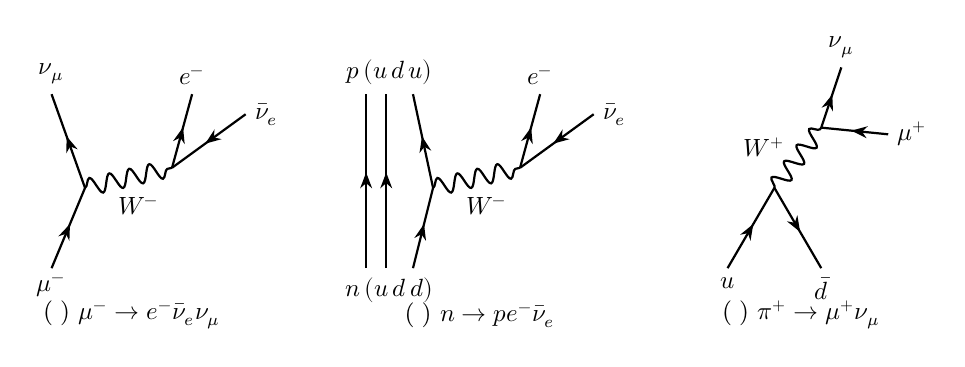
\begin{tikzpicture}[scale=0.85, photon/.style={decorate, decoration={snake, amplitude=1.1mm, segment length=2.6mm}, thick},
  fermion/.style={thick, postaction={decorate}, decoration={markings, mark=at position 0.55 with {\arrow{Stealth[length=2mm]}}}}]
  % распад мюона
  \begin{scope}
   \draw[fermion] (0.5,0) -- (1,1.2); \draw[fermion] (1,1.2) -- (0.5,2.6);
   \draw[photon] (1,1.2) -- (2.3,1.5);
   \draw[fermion] (2.3,1.5) -- (2.6,2.6);
   \draw[fermion] (3.4,2.3) -- (2.3,1.5);
   \node[below, font=\small] at (0.5,0) {$\mu^-$}; \node[above, font=\small] at (0.5,2.6) {$\nu_\mu$};
   \node[above, font=\small] at (2.6,2.6) {$e^-$}; \node[right, font=\small] at (3.4,2.3) {$\bar\nu_e$};
   \node[below, font=\small] at (1.8,1.2) {$W^-$};
   \node[font=\small] at (1.7,-0.7) {(а) $\mu^-\to e^-\bar\nu_e\nu_\mu$};
  \end{scope}
  % распад нейтрона
  \begin{scope}[xshift=5.2cm]
   \draw[fermion] (0.0,0) -- (0.0,2.6); \draw[fermion] (0.3,0) -- (0.3,2.6);
   \draw[fermion] (0.7,0) -- (1.0,1.2); \draw[fermion] (1.0,1.2) -- (0.7,2.6);
   \draw[photon] (1.0,1.2) -- (2.3,1.5);
   \draw[fermion] (2.3,1.5) -- (2.6,2.6);
   \draw[fermion] (3.4,2.3) -- (2.3,1.5);
   \node[below, font=\small] at (0.35,0) {$n\,(u\,d\,d)$}; \node[above, font=\small] at (0.35,2.6) {$p\,(u\,d\,u)$};
   \node[above, font=\small] at (2.6,2.6) {$e^-$}; \node[right, font=\small] at (3.4,2.3) {$\bar\nu_e$};
   \node[below, font=\small] at (1.8,1.2) {$W^-$};
   \node[font=\small] at (1.7,-0.7) {(б) $n\to pe^-\bar\nu_e$};
  \end{scope}
  % распад пиона
  \begin{scope}[xshift=10.4cm]
   \draw[fermion] (0.2,0) -- (0.9,1.2);
   \draw[fermion] (0.9,1.2) -- (1.6,0);
   \draw[photon] (0.9,1.2) -- (1.6,2.1);
   \draw[fermion] (2.6,2.0) -- (1.6,2.1);
   \draw[fermion] (1.6,2.1) -- (1.9,3.0);
   \node[below, font=\small] at (0.2,0) {$u$}; \node[below, font=\small] at (1.6,0) {$\bar d$};
   \node[right, font=\small] at (2.6,2.0) {$\mu^+$}; \node[above, font=\small] at (1.9,3.0) {$\nu_\mu$};
   \node[left, font=\small] at (1.2,1.8) {$W^+$};
   \node[font=\small] at (1.3,-0.7) {(в) $\pi^+\to\mu^+\nu_\mu$};
  \end{scope}
\end{tikzpicture}
\caption{Диаграммы слабых распадов (время — снизу вверх): (а) распад мюона; (б) бета-распад нейтрона на кварковом уровне
($d\to u$, кварки-«наблюдатели» не участвуют); (в) распад $\pi^+$ — аннигиляция $u\bar d$ в виртуальный $W^+$.}
\label{fig:16:decays}
\end{figure}

\subsection{Законы сохранения в слабых процессах}

Сохраняются: энергия, импульс, момент, электрический заряд, барионное число, лептонные числа $L_e$, $L_\mu$, $L_\tau$
(в процессах; нейтринные осцилляции их смешивают). Нарушаются: аромат кварков (странность, очарование и др.),
чётность $P$, зарядовое сопряжение $C$, (слабо) $CP$. Пример запрещённого процесса: $\mu^-\to e^-+\gamma$ (нарушает
$L_e$ и $L_\mu$); экспериментальная доля таких распадов меньше $10^{-12}$.

\section{Математические выводы}

\begin{derivation}[label=der:16:sargent]{закон Сарджента $\Gamma\propto G_F^2E^5$ из размерности}
\emph{Допущения:} энерговыделение $E_0$ (для мюона $E_0\approx m_\mu c^2$) много больше масс продуктов; амплитуда
пропорциональна $G_F$ (низшего порядка), значит ширина $\Gamma\propto G_F^2$.

В единицах $\hbar=c=1$ размерность $[G_F]=\text{энергия}^{-2}$, $[\Gamma]=\text{энергия}$. Единственный оставшийся масштаб — $E_0$.
Следовательно,
\[
  \Gamma=C\,G_F^2E_0^5\qquad(\text{размерность: }E^{-4}\cdot E^5=E).
\]
Безразмерный коэффициент $C$ определяется фазовым объёмом трёх частиц; для распада мюона $C=1/(192\pi^3)$.
Восстанавливая $\hbar$ и $c$: $\Gamma=\dfrac{G_F^2E_0^5}{192\pi^3(\hbar c)^6}$, $\tau=\hbar/\Gamma$.

\emph{Численная проверка для мюона:}
$G_F^2(m_\mu c^2)^5=(1{,}166\cdot10^{-5}\ \text{ГэВ}^{-2})^2\cdot(0{,}10566\ \text{ГэВ})^5=1{,}36\cdot10^{-10}\cdot1{,}316\cdot10^{-5}\ \text{ГэВ}=1{,}79\cdot10^{-15}$~ГэВ;
делим на $192\pi^3=5953$: $\Gamma=3{,}0\cdot10^{-19}$~ГэВ $=3{,}0\cdot10^{-10}$~эВ. Тогда
$\tau=\hbar/\Gamma=6{,}58\cdot10^{-16}\ \text{эВ}\cdot\text{с}/3{,}0\cdot10^{-10}\ \text{эВ}=2{,}2\cdot10^{-6}$~с — совпадает с измеренным временем жизни.
\end{derivation}

\begin{derivation}[label=der:16:tau]{время жизни $\tau$-лептона по универсальности}
Ширина канала $\tau\to e\bar\nu_e\nu_\tau$ вычисляется по той же формуле, что и для мюона, с заменой $m_\mu\to m_\tau$:
$\Gamma(\tau\to e\nu\bar\nu)=\Gamma_\mu(m_\tau/m_\mu)^5$. Если доля этого канала $B_e\approx0{,}178$, то полная ширина
$\Gamma_\tau=\Gamma(\tau\to e\nu\bar\nu)/B_e$, и
\begin{align*}
  \tau_\tau&=\tau_\mu\Bigl(\frac{m_\mu}{m_\tau}\Bigr)^5B_e
  =2{,}197\cdot10^{-6}\ \text{с}\cdot\Bigl(\frac{105{,}66}{1776{,}9}\Bigr)^5\cdot0{,}178\\
  &=2{,}197\cdot10^{-6}\cdot7{,}47\cdot10^{-7}\cdot0{,}178\ \text{с}\approx2{,}9\cdot10^{-13}\ \text{с}.
\end{align*}
Измеренное значение $2{,}90\cdot10^{-13}$~с. Согласие подтверждает лептонную универсальность: $\tau$ и $\mu$ взаимодействуют с
$W$ одинаково. Доля $B_e$ сама объясняется подсчётом каналов: $e\nu\nu$, $\mu\nu\nu$ и $d\bar u$ в трёх цветах — всего
$\approx5$ равноправных каналов, $B_e\approx1/5$.
\end{derivation}

\begin{derivation}[label=der:16:neutron]{оценка времени жизни нейтрона по закону Сарджента}
Сравним с мюоном, считая матричный элемент того же порядка: $\tau_n/\tau_\mu\sim(m_\mu c^2/Q_n)^5$ (с точностью до
множителей фазового объёма, которые для $Q\sim m_ec^2$ отличаются заметно). $(105{,}7/0{,}78)^5\approx(135)^5\approx4{,}5\cdot10^{10}$,
т.\,е. $\tau_n\sim4{,}5\cdot10^{10}\cdot2{,}2\cdot10^{-6}$~с $\sim10^5$~с. Реальное значение 880~с: при $Q\sim m_ec^2$ электрон
нерелятивистский, и закон $Q^5$ лишь грубая оценка; но порядок «очень долго по сравнению с мюоном» объясняется именно малым
энерговыделением. Главный вывод: \emph{время жизни слабых распадов определяется прежде всего энерговыделением}.
\end{derivation}

\begin{derivation}[label=der:16:pion]{кинематика распада $\pi^+\to\mu^+\nu_\mu$}
Пион покоится; продукты разлетаются с равными по модулю импульсами $p$. Сохранение энергии ($m_\nu\approx0$):
\begin{gather*}
  m_\pi c^2=\sqrt{p^2c^2+m_\mu^2c^4}+pc\quad\Longrightarrow\\
  pc=\frac{(m_\pi^2-m_\mu^2)c^2}{2m_\pi}=\frac{139{,}57^2-105{,}66^2}{2\cdot139{,}57}\ \text{МэВ}=29{,}8\ \text{МэВ}.
\end{gather*}
Кинетическая энергия мюона $T_\mu=\sqrt{p^2c^2+m_\mu^2c^4}-m_\mu c^2=4{,}1$~МэВ — моноэнергетический мюон (двухчастичный распад).
Спины: $J_\pi=0$, импульсы противоположны, значит проекции спинов $\mu^+$ и $\nu_\mu$ на свои импульсы одинаковы: левое $\nu_\mu$
требует левого $\mu^+$ — отсюда полная поляризация мюонов от распада пионов.
\end{derivation}

\section{Итоговые формулы}

\keyformula{\frac{G_F}{\sqrt2}=\frac{g^2}{8M_W^2},\qquad \frac{G_F}{(\hbar c)^3}=1{,}166\cdot10^{-5}\ \text{ГэВ}^{-2},\qquad M_Z=\frac{M_W}{\cos\theta_W}}
 {$g$ — константа слабой связи, $\theta_W$ — угол Вайнберга ($\sin^2\theta_W\approx0{,}23$); в первой формуле $\hbar=c=1$.}
 {энергии $\ll M_Wc^2$ (эффективная теория Ферми).}
 {связь константы Ферми с массой переносчика; «слабость» как следствие большой $M_W$.}

\keyformula{\Gamma_\mu=\frac{G_F^2(m_\mu c^2)^5}{192\pi^3(\hbar c)^6},\qquad \Gamma\propto G_F^2E_0^5}
 {$\Gamma=\hbar/\tau$ — ширина, $E_0$ — энерговыделение.}
 {$E_0\gg$ масс продуктов; низший порядок по $G_F$.}
 {время жизни мюона, $\tau$-лептона; оценки времён бета-распадов.}

\keyformula{\mu^-\to e^-\bar\nu_e\nu_\mu,\quad n\to pe^-\bar\nu_e,\quad \pi^+\to\mu^+\nu_\mu,\quad \Lambda\to p\pi^-}
 {$\tau_\mu=2{,}2$~мкс, $\tau_n\approx880$~с, $\tau_{\pi^\pm}=2{,}6\cdot10^{-8}$~с, $\tau_\Lambda=2{,}6\cdot10^{-10}$~с.}
 {сохраняются $Q$, $B$, $L_e$, $L_\mu$; странность меняется на 1 (для $\Lambda$).}
 {типичные слабые распады; проверка законов сохранения.}

\section{Физическая интерпретация}

\textbf{Почему «слабое».} Константа $g$ не мала, но при энергиях $E\ll M_Wc^2$ виртуальный $W$ сильно «вне массовой
поверхности», и амплитуда подавлена множителем $(E/M_Wc^2)^2$. При энергиях LHC слабое взаимодействие по силе
сопоставимо с электромагнитным.

\textbf{Шкала времён жизни.} При одной константе времена слабых распадов различаются на 13 порядков (от
$3\cdot10^{-13}$~с для $\tau$ до 880~с для нейтрона) — из-за степени $E_0^5$ и подавлений (Кабиббо, спиральность).

\textbf{Асимметрия природы.} Нарушение $P$ и $C$ означает, что «зеркальный мир» и «мир из антивещества» по отдельности
физически отличимы от нашего; нарушение $CP$ — одно из условий (Сахаров, 1967) возникновения барионной асимметрии
Вселенной, хотя величины $CP$-нарушения в СМ для её объяснения недостаточно.

\section{Что необходимо знать на экзамене}

\begin{examcheck}
\checkhead{Определения}
\begin{itemize}
 \item слабое взаимодействие: участники, переносчики $W^\pm$, $Z^0$ (массы, спин 1), заряженные и нейтральные токи;
 \item спиральность; нарушение чётности (опыт Ву); угол Кабиббо; лептонные числа.
\end{itemize}
\checkhead{Формулы}
\begin{itemize}
 \item $r_W=\hbar/M_Wc$; $G_F/\sqrt2=g^2/8M_W^2$; $M_Z=M_W/\cos\theta_W$;
 \item $\Gamma\propto G_F^2E_0^5$ (закон Сарджента), $\tau_\tau=\tau_\mu(m_\mu/m_\tau)^5B_e$.
\end{itemize}
\checkhead{Выводы}
\begin{itemize}
 \item закон Сарджента из размерности и численная проверка для мюона;
 \item время жизни $\tau$-лептона по универсальности; кинематика $\pi\to\mu\nu$ и спиральное подавление $\pi\to e\nu$.
\end{itemize}
\checkhead{Интерпретации}
\begin{itemize}
 \item кварковые диаграммы распадов $n$, $\pi^+$, $\Lambda$; почему странные частицы рождаются быстро, а распадаются медленно;
 \item электрослабое объединение и открытие $W$, $Z$, нейтральных токов; три поколения нейтрино по ширине $Z$.
\end{itemize}
\end{examcheck}

% ======================================================================
\chapter[Атомное ядро. Радиус ядра. Формула Вайцзеккера]%
        {Атомное ядро. Радиус ядра. Формула Вайцзеккера}
\label{t:17}
% ======================================================================

\begin{qbox}
\textbf{Билет 17.} Атомное ядро, зависимость радиуса от массового числа. Формула Вайцзеккера
для энергии связи ядра.
\end{qbox}

\section{Содержание билета}

\textbf{Подтемы:}
\begin{enumerate}
 \item состав ядра, обозначения, изотопы/изобары/изотоны; свойства ядерных сил;
 \item размеры ядер: методы измерения, закон $R=r_0A^{1/3}$, распределение плотности, постоянство плотности;
 \item дефект массы и энергия связи; удельная энергия связи и её зависимость от $A$;
 \item капельная модель и полуэмпирическая формула Вайцзеккера: смысл и обоснование каждого члена;
 \item следствия: долина стабильности, энергетика деления и синтеза.
\end{enumerate}

\textbf{Необходимые понятия:} $E=mc^2$; электростатическая энергия заряженного шара; газ Ферми
(\tref{t:04}: число состояний в фазовом объёме; \tref{t:13}: принцип Паули); сильное взаимодействие (\tref{t:15}).

\section{Определения и физические принципы}

\begin{definition}[ядро]
Атомное ядро — связанная система $Z$ протонов и $N$ нейтронов (нуклонов); $A=Z+N$ — массовое число.
Обозначение $\nuc{X}{A}{Z}$ (например, $\nuc{U}{238}{92}$). \emph{Изотопы} — одинаковые $Z$, \emph{изобары} — одинаковые $A$,
\emph{изотоны} — одинаковые $N$.
\end{definition}

\begin{definition}[энергия связи]
Энергия, необходимая для разделения ядра на свободные нуклоны:
\begin{equation}\label{eq:17:Eb}
  E_{\text{св}}(A,Z)=\bigl[Zm_p+Nm_n-M_{\text{я}}(A,Z)\bigr]c^2=\bigl[ZM(\nucl{H}{1})+Nm_n-M_{\text{ат}}(A,Z)\bigr]c^2,
\end{equation}
где во втором выражении использованы массы нейтральных атомов (массы электронов сокращаются; разностью
энергий связи электронов пренебрегаем). Величина $\Delta M=E_{\text{св}}/c^2$ — \emph{дефект массы};
$\varepsilon=E_{\text{св}}/A$ — \emph{удельная энергия связи}.
\end{definition}

\begin{definition}[свойства ядерных сил]
Ядерные силы — сильное (остаточное цветовое) взаимодействие нуклонов: (1) короткодействующие, радиус
$\sim1{,}5$--$2$~фм; (2) притягивающие на расстояниях $\sim1$~фм и отталкивающие на расстояниях $\lesssim0{,}5$~фм (кор);
(3) зарядово-независимые ($pp\approx nn\approx np$); (4) спин-зависимые и нецентральные; (5) обладают свойством
\emph{насыщения}: нуклон взаимодействует лишь с ближайшими соседями.
\end{definition}

\emph{Область применимости.} Формула Вайцзеккера — полуэмпирическая (капельная модель); она хорошо описывает
энергии связи средних и тяжёлых ядер (точность порядка 1\,\% и лучше), но не воспроизводит оболочечные эффекты
(магические числа 2, 8, 20, 28, 50, 82, 126) и неприменима к самым лёгким ядрам.

\section{Основная теория}

\subsection{Размеры ядер}

\paragraph{Методы.}
\begin{enumerate}
 \item \textbf{Рассеяние $\alpha$-частиц} (Резерфорд): отклонения от формулы Резерфорда при больших энергиях и углах
       начинаются, когда частица подходит к ядру на расстояние действия ядерных сил.
 \item \textbf{Рассеяние быстрых электронов} (Хофштадтер, 1950-е; Нобелевская премия 1961): электроны с $\lambda\sim1$~фм
       (энергии сотни МэВ) не чувствуют ядерных сил; дифракционная картина даёт распределение \emph{заряда} в ядре.
 \item \textbf{Мюонные атомы} (\tref{t:03}): уровни мюона, проводящего часть времени внутри ядра, сдвинуты относительно
       точечного ядра.
 \item \textbf{Зеркальные ядра} (вывод~\ref{der:17:mirror}): разность энергий связи пар ($\nucl{N}{15}$--$\nucl{O}{15}$ и др.) обусловлена
       кулоновской энергией и даёт $R$.
 \item \textbf{Рассеяние нейтронов} и времена жизни $\alpha$-распада — радиус действия ядерных сил.
\end{enumerate}

\paragraph{Результат.} Все методы дают
\begin{equation}\label{eq:17:R}
  R=r_0A^{1/3},\qquad r_0\approx1{,}2\ \text{фм (по распределению заряда)},\quad 1{,}3\text{--}1{,}4\ \text{фм (по ядерным силам)}.
\end{equation}
Различие связано с тем, что ядерные силы действуют на некотором расстоянии за пределами распределения
нуклонов. Объём ядра пропорционален числу нуклонов: $V=\frac43\pi r_0^3A$, т.\,е. \emph{плотность ядерного вещества
одинакова для всех ядер} (вывод~\ref{der:17:density}):
\[
  n\approx\frac{3}{4\pi r_0^3}\approx0{,}14\text{--}0{,}17\ \text{фм}^{-3},\qquad \rho\approx2{,}3\cdot10^{14}\ \text{г/см}^3.
\]
Это прямое следствие насыщения ядерных сил и отталкивания на малых расстояниях: нуклоны «упакованы» как молекулы
в капле жидкости.

\paragraph{Распределение плотности} (из рассеяния электронов) описывается распределением Ферми
\begin{equation}\label{eq:17:fermi}
  \rho(r)=\frac{\rho_0}{1+\exp\bigl((r-c)/a\bigr)},\qquad c\approx1{,}07A^{1/3}\ \text{фм},\quad a\approx0{,}55\ \text{фм}:
\end{equation}
почти постоянная плотность в центре и размытый поверхностный слой толщиной $t\approx4{,}4a\approx2{,}4$~фм (спад
от 90 до 10\,\% $\rho_0$) — одинаковой для всех ядер (рис.~\ref{fig:17:fermi}).

\begin{figure}[htbp]
\centering
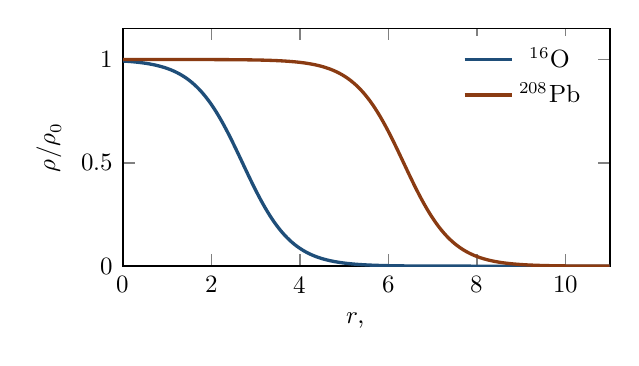
\begin{tikzpicture}
\begin{axis}[width=0.64\linewidth, height=4.6cm, xlabel={$r$, фм}, ylabel={$\rho/\rho_0$}, xmin=0, xmax=11, ymin=0, ymax=1.15,
   samples=200, legend style={font=\small, draw=none}, legend pos=north east]
  \addplot[very thick, accent, domain=0:11] {1/(1+exp((x-1.07*16^(1/3))/0.55))};
  \addlegendentry{$^{16}$O}
  \addplot[very thick, keycol, domain=0:11] {1/(1+exp((x-1.07*208^(1/3))/0.55))};
  \addlegendentry{$^{208}$Pb}
\end{axis}
\end{tikzpicture}
\caption{Распределение Ферми~\eqref{eq:17:fermi} для лёгкого и тяжёлого ядер (расчёт по формуле с $c=1{,}07A^{1/3}$~фм,
$a=0{,}55$~фм). Центральная плотность одинакова, толщина поверхностного слоя одинакова.}
\label{fig:17:fermi}
\end{figure}

\subsection{Энергия связи. Удельная энергия связи}

Примеры: дейтрон — $2{,}22$~МэВ ($1{,}11$~МэВ/нуклон); $\nucl{He}{4}$ — $28{,}3$~МэВ ($7{,}07$~МэВ/нуклон); $\nucl{Fe}{56}$ — $8{,}79$~МэВ/нуклон;
$\nucl{U}{238}$ — $7{,}57$~МэВ/нуклон. Основные закономерности:
\begin{itemize}
 \item для $A\gtrsim20$ удельная энергия связи почти постоянна, $\varepsilon\approx7{,}5$--$8{,}8$~МэВ, т.\,е. $E_{\text{св}}\propto A$ —
       ещё одно проявление насыщения (если бы каждый нуклон взаимодействовал со всеми, было бы $E_{\text{св}}\propto A^2$);
 \item максимум $\varepsilon$ в области железа--никеля ($A\approx56$--$62$); слева — рост, справа — плавный спад;
 \item у лёгких ядер $\varepsilon$ меньше и испытывает скачки (особо устойчивы $\nucl{He}{4}$, $\nucl{C}{12}$, $\nucl{O}{16}$).
\end{itemize}
Энергия связи — около 1\,\% энергии покоя ядра ($8\MeV/939\MeV$), тогда как в атоме — $\sim10^{-8}$.

\subsection{Капельная модель и формула Вайцзеккера}

Постоянство плотности и насыщение сил делают ядро похожим на каплю несжимаемой заряженной жидкости. Энергия связи
складывается из вкладов, каждый из которых имеет ясную физическую природу (К.~Вайцзеккер, 1935):
\begin{equation}\label{eq:17:SEMF}
  \boxed{E_{\text{св}}(A,Z)=a_VA-a_SA^{2/3}-a_C\frac{Z^2}{A^{1/3}}-a_A\frac{(A-2Z)^2}{A}+\delta(A,Z)}
\end{equation}
\begin{enumerate}
 \item \textbf{Объёмная энергия} $a_VA$: каждый нуклон связан с фиксированным числом соседей (насыщение) и даёт
       одинаковый вклад; $E\propto V\propto A$.
 \item \textbf{Поверхностная энергия} $-a_SA^{2/3}$: нуклоны на поверхности имеют меньше соседей и связаны слабее; поправка
       пропорциональна площади $4\pi R^2\propto A^{2/3}$ (аналог поверхностного натяжения). Относительно наиболее важна для лёгких ядер.
 \item \textbf{Кулоновская энергия} $-a_CZ^2/A^{1/3}$: электростатическое отталкивание протонов, равномерно распределённых по шару
       радиуса $R=r_0A^{1/3}$: $E_C=\frac35\frac{Z^2e^2}{R}$ (вывод~\ref{der:17:coulomb}); $a_C=\frac{3e^2}{5r_0}\approx0{,}7$~МэВ. (Иногда пишут
       $Z(Z-1)$, исключая самодействие протона.) Определяет спад $\varepsilon$ у тяжёлых ядер.
 \item \textbf{Энергия симметрии (асимметрии)} $-a_A(N-Z)^2/A$: при заданном $A$ энергетически выгодно $N=Z$. Причина —
       принцип Паули: протоны и нейтроны заполняют отдельные системы уровней, и избыток частиц одного сорта
       вынужден занимать более высокие уровни (вывод~\ref{der:17:asym}). Форма $(N-Z)^2/A$ следует из модели газа Ферми.
 \item \textbf{Энергия спаривания} $\delta$: нуклоны одного сорта образуют пары с противоположными спинами, что дополнительно
       выгодно:
       \[
         \delta=\begin{cases}+a_PA^{-3/4}, & Z,N\ \text{чётные (чётно-чётные ядра)},\\ 0, & A\ \text{нечётное},\\ -a_PA^{-3/4}, & Z,N\ \text{нечётные}.\end{cases}
       \]
       Поэтому стабильные нечётно-нечётные ядра почти отсутствуют (лишь $\nucl{H}{2}$, $\nucl{Li}{6}$, $\nucl{B}{10}$, $\nucl{N}{14}$).
\end{enumerate}
Один из распространённых наборов коэффициентов (подбираются по экспериментальным массам; разные авторы дают немного
различающиеся значения):
\begin{equation}\label{eq:17:coef}
  a_V=15{,}75,\quad a_S=17{,}8,\quad a_C=0{,}711,\quad a_A=23{,}7,\quad a_P=34\ \ \text{(МэВ)}.
\end{equation}
Проверка для $\nucl{Fe}{56}$ и $\nucl{U}{238}$ — в выводе~\ref{der:17:check}. Вклады членов в $\varepsilon(A)$ показаны на рис.~\ref{fig:17:BA}.

\begin{figure}[htbp]
\centering
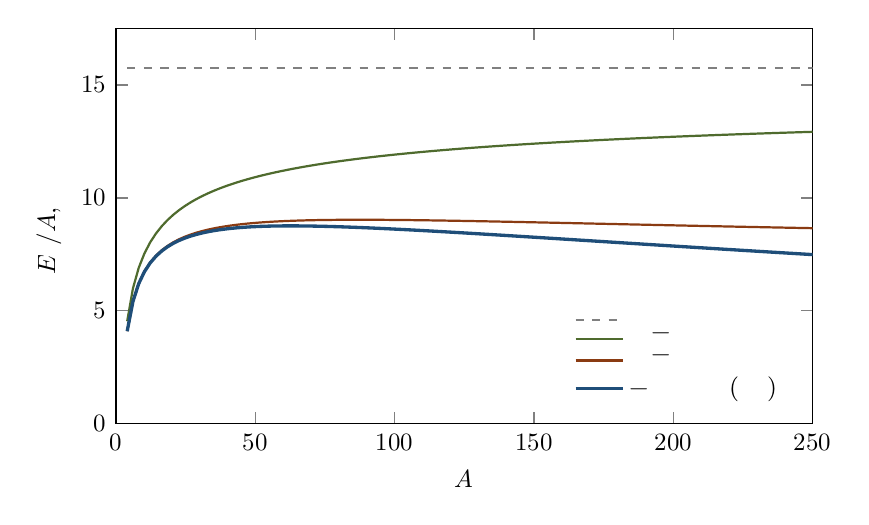
\begin{tikzpicture}
\begin{axis}[width=0.86\linewidth, height=6.6cm, xlabel={$A$}, ylabel={$E_{\text{св}}/A$, МэВ}, xmin=0, xmax=250, ymin=0, ymax=17.5,
   samples=120, legend style={font=\small, draw=none, fill=white, fill opacity=0.85, text opacity=1}, legend pos=south east,
   declare function={Z0(\A)=\A/(1.98+0.0149*\A^(2/3));}]
  \addplot[gray, thick, dashed, domain=4:250] {15.75};
  \addlegendentry{объёмный член}
  \addplot[dercol, thick, domain=4:250] {15.75-17.8*x^(-1/3)};
  \addlegendentry{$-$ поверхность}
  \addplot[keycol, thick, domain=4:250] {15.75-17.8*x^(-1/3)-0.711*Z0(x)^2/x^(4/3)};
  \addlegendentry{$-$ кулоновский}
  \addplot[accent, very thick, domain=4:250] {15.75-17.8*x^(-1/3)-0.711*Z0(x)^2/x^(4/3)-23.7*(x-2*Z0(x))^2/x^2};
  \addlegendentry{$-$ симметрия (итог)}
\end{axis}
\end{tikzpicture}
\caption{Удельная энергия связи по формуле Вайцзеккера (без члена спаривания) вдоль долины стабильности $Z=Z_0(A)$
и вклады отдельных членов (расчёт по коэффициентам~\eqref{eq:17:coef}). Максимум $\approx8{,}8$~МэВ при $A\approx60$;
для лёгких ядер формула неточна.}
\label{fig:17:BA}
\end{figure}

\subsection{Следствия формулы Вайцзеккера}

\paragraph{Долина стабильности.} Масса ядра при фиксированном $A$ — парабола по $Z$ (вывод~\ref{der:17:valley}); её минимум
\begin{equation}\label{eq:17:Z0}
  Z_0(A)\approx\frac{A}{1{,}98+0{,}015A^{2/3}}.
\end{equation}
Для лёгких ядер $Z_0\approx A/2$ ($N\approx Z$), для тяжёлых кулоновское отталкивание сдвигает стабильность к избытку
нейтронов ($\nucl{U}{238}$: $Z_0\approx93$, реально $Z=92$, $N/Z\approx1{,}6$). Ядра выше и ниже долины испытывают бета-распады
(\tref{t:20}).

\paragraph{Энергетика деления и синтеза.} Из хода $\varepsilon(A)$: при делении тяжёлого ядра ($\varepsilon\approx7{,}6$~МэВ) на два средних
($\varepsilon\approx8{,}5$~МэВ) выделяется $\approx0{,}9\cdot236\approx200$~МэВ; при синтезе лёгких ядер ($\nucl{H}{2}+\nucl{H}{3}\to\nucl{He}{4}+n$) —
$17{,}6$~МэВ, т.\,е. больше на нуклон. Деление энергетически выгодно, когда кулоновская энергия велика по сравнению с
поверхностной; параметр делимости $Z^2/A$: при $Z^2/A\gtrsim2a_S/a_C\approx50$ ядро неустойчиво к делению мгновенно.

\paragraph{Альфа-распад} энергетически возможен для $A\gtrsim150$ (\tref{t:19}): энергия связи $\alpha$-частицы ($28{,}3$~МэВ)
превышает $4\varepsilon$ тяжёлого ядра.

\section{Математические выводы}

\begin{derivation}[label=der:17:density]{плотность ядерного вещества}
Число нуклонов в единице объёма:
\[
  n=\frac{A}{\frac43\pi R^3}=\frac{A}{\frac43\pi r_0^3A}=\frac{3}{4\pi r_0^3}=\frac{3}{4\pi(1{,}2\ \text{фм})^3}\approx0{,}14\ \text{фм}^{-3}
\]
— от $A$ не зависит. Массовая плотность $\rho=nm_N=0{,}14\cdot10^{39}\ \text{см}^{-3}\cdot1{,}67\cdot10^{-24}\ \text{г}\approx2{,}3\cdot10^{14}$~г/см$^3$
(центральная плотность из~\eqref{eq:17:fermi} немного выше, $\approx0{,}16$~фм$^{-3}$). Среднее расстояние между нуклонами
$n^{-1/3}\approx1{,}9$~фм — порядка радиуса ядерных сил.
\end{derivation}

\begin{derivation}[label=der:17:coulomb]{кулоновская энергия равномерно заряженного шара}
Соберём шар радиуса $R$ с зарядом $Q$ послойно. Когда уже собран шар радиуса $r$ с зарядом $q(r)=Q r^3/R^3$, доставка из
бесконечности слоя $\dd q=3Qr^2\dd r/R^3$ требует работы $\dd W=q(r)\,\dd q/r$. Тогда
\[
  E_C=\int_0^R\frac{q(r)}{r}\dd q=\int_0^R\frac{Qr^3}{R^3r}\cdot\frac{3Qr^2}{R^3}\dd r=\frac{3Q^2}{R^6}\int_0^Rr^4\dd r=\frac35\frac{Q^2}{R}.
\]
При $Q=Ze$, $R=r_0A^{1/3}$: $E_C=\dfrac{3e^2}{5r_0}\dfrac{Z^2}{A^{1/3}}$, т.\,е. $a_C=\dfrac{3}{5}\dfrac{e^2}{r_0}=0{,}6\cdot\dfrac{1{,}44\ \text{МэВ}\cdot\text{фм}}{1{,}2\ \text{фм}}=0{,}72$~МэВ —
в согласии с эмпирическим $0{,}71$~МэВ.
\end{derivation}

\begin{derivation}[label=der:17:asym]{энергия симметрии в модели газа Ферми}
\emph{Допущения:} нуклоны — свободные фермионы со спином $\frac12$ в объёме $V$ ядра; протоны и нейтроны — две независимые
системы; учитывается только кинетическая энергия.

\emph{Шаг 1.} Число состояний с импульсом меньше $p_F$: $2\cdot V\cdot\frac43\pi p_F^3/(2\pi\hbar)^3$ (множитель 2 — спин). Приравняв числу
частиц $N$: $p_F=\hbar(3\pi^2N/V)^{1/3}$, $\varepsilon_F=p_F^2/2m$.

\emph{Шаг 2.} Средняя кинетическая энергия частицы $\frac35\varepsilon_F$, полная $E=\frac35N\varepsilon_F\propto N^{5/3}/V^{2/3}$. Для двух сортов:
\[
  E_{\text{кин}}=C\,\frac{N^{5/3}+Z^{5/3}}{A^{2/3}},\qquad C=\frac35\frac{\hbar^2}{2m}\Bigl(\frac{3\pi^2}{\frac43\pi r_0^3}\Bigr)^{2/3}\quad(V\propto A).
\]
\emph{Шаг 3.} Положим $N=\frac A2(1+\eta)$, $Z=\frac A2(1-\eta)$, $\eta=(N-Z)/A$. Разложение до $\eta^2$:
$(1\pm\eta)^{5/3}\approx1\pm\frac53\eta+\frac59\eta^2$, поэтому
\[
  N^{5/3}+Z^{5/3}=\Bigl(\frac A2\Bigr)^{5/3}\Bigl(2+\frac{10}{9}\eta^2\Bigr).
\]
\emph{Шаг 4.} Отсюда $E_{\text{кин}}=E_0\bigl(1+\frac59\eta^2\bigr)$, где $E_0=\frac35A\varepsilon_F^{(0)}$ — энергия симметричного ядра ($\varepsilon_F^{(0)}$ —
энергия Ферми при $N=Z$). Добавка
\[
  \Delta E=\frac35A\varepsilon_F^{(0)}\cdot\frac59\eta^2=\frac{\varepsilon_F^{(0)}}{3}\frac{(N-Z)^2}{A}.
\]
При $\varepsilon_F^{(0)}\approx37$~МэВ кинетический вклад $\approx12$~МэВ — около половины эмпирического $a_A$; остальное даёт зависимость
ядерного взаимодействия от изоспина ($np$-притяжение сильнее). Главное — модель объясняет \emph{форму} $(N-Z)^2/A$.
\end{derivation}

\begin{derivation}[label=der:17:valley]{долина стабильности}
Масса атома $M(A,Z)c^2=Zm_{\mathrm H}c^2+(A-Z)m_nc^2-E_{\text{св}}(A,Z)$ (с массой атома водорода). При фиксированном $A$:
\[
  \pdiff{M}{Z}c^2=(m_{\mathrm H}-m_n)c^2+\frac{2a_CZ}{A^{1/3}}-\frac{4a_A(A-2Z)}{A}=0 .
\]
Решая относительно $Z$, с $(m_n-m_{\mathrm H})c^2=0{,}78$~МэВ:
\[
  Z_0=\frac{4a_A+0{,}78}{\dfrac{8a_A}{A}+\dfrac{2a_C}{A^{1/3}}}=\frac{A}{\dfrac{8a_A}{4a_A+0{,}78}+\dfrac{2a_C}{4a_A+0{,}78}A^{2/3}}
  =\frac{A}{1{,}98+0{,}0149A^{2/3}}.
\]
Поскольку $M$ квадратична по $Z$, изобары лежат на параболе $M(Z)=M(Z_0)+\frac12\bigl(\frac{8a_A}{A}+\frac{2a_C}{A^{1/3}}\bigr)(Z-Z_0)^2/c^2$
(плюс член спаривания).
\end{derivation}

\begin{derivation}[label=der:17:mirror]{радиус по зеркальным ядрам}
Зеркальные ядра (например, $\nucl{N}{15}$: $Z=7$, $N=8$ и $\nucl{O}{15}$: $Z=8$, $N=7$) отличаются заменой $p\leftrightarrow n$. Из-за
зарядовой независимости ядерные энергии одинаковы, и разность энергий связи равна разности кулоновских:
\[
  \Delta E_C=\frac35\frac{e^2}{R}\bigl[Z^2-(Z-1)^2\bigr]=\frac35\frac{e^2}{R}(2Z-1).
\]
Измерив $\Delta E_C$ (по энергии $\beta^+$-распада $Z\to Z-1$ с учётом $m_n-m_p$), находим $R$. Результат согласуется с $r_0\approx1{,}2$--$1{,}3$~фм.
\end{derivation}

\begin{derivation}[label=der:17:check]{численная проверка формулы}
\emph{$\nucl{Fe}{56}$} ($Z=26$, $A^{1/3}=3{,}826$, $A^{2/3}=14{,}64$, чётно-чётное):
$15{,}75\cdot56=882{,}0$; $17{,}8\cdot14{,}64=260{,}6$; $0{,}711\cdot676/3{,}826=125{,}6$; $23{,}7\cdot16/56=6{,}8$; $\delta=34/56^{3/4}=1{,}7$.
$E_{\text{св}}\approx882{,}0-260{,}6-125{,}6-6{,}8+1{,}7=490{,}7$~МэВ, $\varepsilon\approx8{,}76$~МэВ (опыт: 492,3~МэВ; 8,79).

\emph{$\nucl{U}{238}$} ($Z=92$, $A^{1/3}=6{,}197$, $A^{2/3}=38{,}40$): $3748{,}5-683{,}5-971{,}1-290{,}4+0{,}6=1804$~МэВ, $\varepsilon\approx7{,}58$~МэВ
(опыт: 7,57). Пять параметров описывают энергии связи сотен ядер с точностью $\sim0{,}5$--$1\,\%$.
\end{derivation}

\section{Итоговые формулы}

\keyformula{R=r_0A^{1/3},\qquad r_0\approx1{,}2\text{--}1{,}4\ \text{фм},\qquad n=\frac{3}{4\pi r_0^3}\approx0{,}15\ \text{фм}^{-3}}
 {$A$ — массовое число; $n$ — концентрация нуклонов.}
 {все ядра, кроме самых лёгких; $r_0$ зависит от метода (заряд или ядерные силы).}
 {размер ядра; постоянство ядерной плотности.}

\keyformula{E_{\text{св}}=\bigl[Zm_{\mathrm H}+Nm_n-M_{\text{ат}}\bigr]c^2}
 {$m_{\mathrm H}$ — масса атома водорода, $M_{\text{ат}}$ — масса атома.}
 {точно (с пренебрежением разностью электронных энергий связи).}
 {энергия связи по таблицам масс; энерговыделение реакций.}

\keyformula{E_{\text{св}}=a_VA-a_SA^{2/3}-a_C\frac{Z^2}{A^{1/3}}-a_A\frac{(A-2Z)^2}{A}+\delta}
 {$a_V\approx15{,}8$, $a_S\approx17{,}8$, $a_C\approx0{,}71$, $a_A\approx23{,}7$~МэВ; $\delta=\pm34A^{-3/4}$~МэВ или 0.}
 {средние и тяжёлые ядра; без оболочечных поправок.}
 {энергии связи, массы, долина стабильности, энергии $\alpha$- и $\beta$-распадов, деления.}

\keyformula{a_C=\frac35\frac{e^2}{r_0},\qquad Z_0\approx\frac{A}{1{,}98+0{,}015A^{2/3}}}
 {$e^2=1{,}44$~МэВ$\cdot$фм; $Z_0$ — заряд наиболее стабильного изобара.}
 {капельная модель.}
 {связь коэффициента с радиусом; положение стабильных ядер.}

\section{Физическая интерпретация}

\textbf{Насыщение.} Пропорциональность $V\propto A$ и $E_{\text{св}}\propto A$ — два независимых проявления того, что ядерные силы
короткодействующие и насыщаются; без отталкивания на малых расстояниях ядро сжималось бы с ростом $A$.

\textbf{Конкуренция членов.} Поверхностный член уменьшает $\varepsilon$ у лёгких ядер, кулоновский — у тяжёлых; отсюда максимум
около железа. Это определяет и источники ядерной энергии (деление тяжёлых, синтез лёгких), и конечный продукт
звёздного нуклеосинтеза (железный пик). Существование тяжёлых ядер ограничено кулоновским отталкиванием (деление,
$\alpha$-распад).

\textbf{Ограничения модели.} Отклонения от формулы Вайцзеккера на несколько МэВ вблизи магических чисел указывают на
оболочечную структуру ядра — нуклоны движутся в общем потенциале почти независимо, как электроны в атоме.

\section{Что необходимо знать на экзамене}

\begin{examcheck}
\checkhead{Определения}
\begin{itemize}
 \item состав ядра, изотопы/изобары/изотоны; свойства ядерных сил (насыщение!);
 \item дефект массы, энергия связи, удельная энергия связи.
\end{itemize}
\checkhead{Формулы}
\begin{itemize}
 \item $R=r_0A^{1/3}$, $r_0\approx1{,}2$~фм; $n\approx0{,}15$~фм$^{-3}$; распределение Ферми (качественно);
 \item формула Вайцзеккера со всеми пятью членами и порядками коэффициентов; $Z_0(A)$.
\end{itemize}
\checkhead{Выводы}
\begin{itemize}
 \item постоянство плотности из $R\propto A^{1/3}$; кулоновская энергия шара $\frac35Q^2/R$ и оценка $a_C$;
 \item форма энергии симметрии из газа Ферми; долина стабильности; (желательно) метод зеркальных ядер.
\end{itemize}
\checkhead{Интерпретации}
\begin{itemize}
 \item физический смысл каждого члена; ход кривой $\varepsilon(A)$ и максимум у Fe;
 \item энергия деления ($\sim200$~МэВ) и синтеза; почему тяжёлые ядра нейтроноизбыточны; методы измерения $R$.
\end{itemize}
\end{examcheck}

% ======================================================================
\chapter[Радиоактивность. Закон распада. Вековое уравнение]%
        {Ядерная радиоактивность. Закон радиоактивного распада. Вековое уравнение}
\label{t:18}
% ======================================================================

\begin{qbox}
\textbf{Билет 18.} Ядерная радиоактивность. Закон радиоактивного распада, константа распада,
период полураспада, среднее время жизни, вековое уравнение.
\end{qbox}

\section{Содержание билета}

\textbf{Подтемы:}
\begin{enumerate}
 \item явление радиоактивности, виды распадов, их общие свойства;
 \item закон радиоактивного распада: вывод из статистической гипотезы, постоянная распада;
 \item период полураспада, среднее время жизни и связь между ними; активность и её единицы;
 \item последовательные распады (цепочки): решение уравнений, вековое (секулярное) и подвижное равновесие; вековое уравнение;
 \item применения: радиоактивные семейства, датирование, определение больших периодов полураспада.
\end{enumerate}

\textbf{Необходимые понятия:} энергия связи и стабильность ядер (\tref{t:17}); вероятность, распределение
Пуассона; линейные дифференциальные уравнения первого порядка; ширина уровня и время жизни (\tref{t:02}).

\section{Определения и физические принципы}

\begin{definition}[радиоактивность]
Самопроизвольное (спонтанное) превращение неустойчивых атомных ядер в другие ядра, сопровождающееся испусканием
частиц или излучения. Основные виды: $\alpha$-распад (испускание ядра $\nucl{He}{4}$), $\beta$-распад ($\beta^-$, $\beta^+$, электронный
захват), $\gamma$-излучение (переход ядра между уровнями), спонтанное деление; реже — испускание протонов, кластеров.
\end{definition}

\begin{definition}[постоянная распада]
\emph{Постоянная распада} $\lambda$ — вероятность распада одного ядра в единицу времени: вероятность распасться за малый
интервал $\dd t$ равна $\lambda\,\dd t$. Размерность $[\lambda]=\text{с}^{-1}$.
\end{definition}

\begin{definition}[период полураспада, среднее время жизни, активность]
\emph{Период полураспада} $T_{1/2}$ — время, за которое распадается половина имеющихся ядер. \emph{Среднее время жизни}
$\tau$ — среднее значение времени существования ядра до распада. \emph{Активность} $\mathcal A$ — число распадов в единицу
времени: $\mathcal A=-\dd N/\dd t=\lambda N$. Единицы: беккерель (1~Бк $=1$ распад/с) и кюри (1~Ки $=3{,}7\cdot10^{10}$~Бк —
примерно активность 1~г $\nucl{Ra}{226}$).
\end{definition}

\emph{Физический смысл.} Радиоактивный распад — квантовый переход из квазистационарного состояния; момент распада
отдельного ядра принципиально непредсказуем, определена лишь вероятность. Постоянная $\lambda$ — свойство ядра:
она не зависит от времени существования ядра (ядра «не стареют»), от температуры, давления, химического состояния
(за исключением слабой зависимости для электронного захвата и внутренней конверсии, где важна плотность электронов
у ядра, — эффекты порядка $10^{-3}$).

\emph{Область применимости закона.} Экспоненциальный закон описывает поведение большого числа ядер в среднем; при
малых $N$ существенны флуктуации (распределение Пуассона, относительная погрешность $1/\sqrt{N_{\text{расп}}}$).

\section{Основная теория}

\subsection{Открытие и виды распадов}

А.~Беккерель (1896) обнаружил излучение солей урана; М.~и П.~Кюри открыли полоний и радий; Э.~Резерфорд разделил
излучение на $\alpha$, $\beta$, $\gamma$ по отклонению в магнитном поле и установил (вместе с Ф.~Содди, 1902), что радиоактивность —
превращение одних элементов в другие. Правила смещения: при $\alpha$-распаде $(A,Z)\to(A-4,Z-2)$, при $\beta^-$-распаде
$(A,Z)\to(A,Z+1)$, при $\beta^+$-распаде и электронном захвате $(A,Z)\to(A,Z-1)$, при $\gamma$-переходе $A$ и $Z$ не меняются.

Периоды полураспада лежат в огромном диапазоне: от $\sim10^{-22}$~с до $\gtrsim10^{24}$~лет ($\nucl{Te}{128}$, двойной бета-распад).
Причины: экспоненциальная зависимость вероятности туннелирования для $\alpha$-распада (\tref{t:19}), сильная зависимость
от энергии ($\propto Q^5$) и правил отбора для $\beta$-распада (\tref{t:20}).

\subsection{Закон радиоактивного распада}

Из определения постоянной распада (вывод~\ref{der:18:law}):
\begin{equation}\label{eq:18:law}
  \diff{N}{t}=-\lambda N\quad\Longrightarrow\quad N(t)=N_0\,\ee^{-\lambda t}=N_0\,2^{-t/T_{1/2}} .
\end{equation}
Связь характерных времён (вывод~\ref{der:18:tau}):
\begin{equation}\label{eq:18:times}
  T_{1/2}=\frac{\ln2}{\lambda}\approx\frac{0{,}693}{\lambda},\qquad \tau=\frac1\lambda,\qquad T_{1/2}=\tau\ln2 .
\end{equation}
За время $\tau$ число ядер уменьшается в $\ee$ раз. Активность убывает по тому же закону: $\mathcal A(t)=\lambda N_0\ee^{-\lambda t}$.
Измеряя $\mathcal A$ в разные моменты, определяют $\lambda$ по наклону прямой $\ln\mathcal A(t)$ (для коротких периодов); для
очень больших $T_{1/2}$ используют $\lambda=\mathcal A/N$ при известном числе ядер.

\paragraph{Связь с шириной уровня.} Квазистационарное состояние со временем жизни $\tau$ имеет энергетическую ширину
$\Gamma=\hbar/\tau=\hbar\lambda$; $|\Psi|^2\propto\ee^{-t/\tau}$. Это связывает закон распада с соотношением энергия--время (\tref{t:02}).

\paragraph{Несколько каналов распада.} Если ядро распадается несколькими способами с постоянными $\lambda_i$, то полная
постоянная $\lambda=\sum_i\lambda_i$ (вероятности несовместных событий складываются), а доля канала $i$ (коэффициент
ветвления) равна $\lambda_i/\lambda$. Время жизни определяется полной $\lambda$.

\begin{figure}[htbp]
\centering
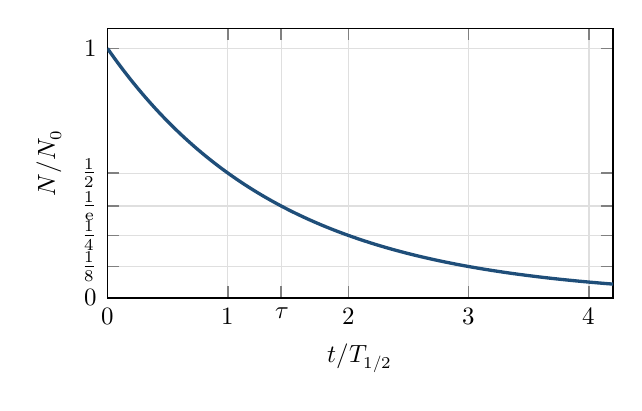
\begin{tikzpicture}
\begin{axis}[width=0.66\linewidth, height=5.0cm, xlabel={$t/T_{1/2}$}, ylabel={$N/N_0$}, xmin=0, xmax=4.2, ymin=0, ymax=1.08,
   samples=150, xtick={0,1,1.4427,2,3,4}, xticklabels={$0$,$1$,$\tau$,$2$,$3$,$4$}, ytick={0,0.125,0.25,0.3679,0.5,1},
   yticklabels={$0$,$\frac18$,$\frac14$,$\frac1{\ee}$,$\frac12$,$1$}, grid=major, grid style={gray!25}]
  \addplot[very thick, accent, domain=0:4.2] {2^(-x)};
\end{axis}
\end{tikzpicture}
\caption{Закон радиоактивного распада $N/N_0=2^{-t/T_{1/2}}$. Отмечены период полураспада и среднее время жизни
$\tau=T_{1/2}/\ln2\approx1{,}44\,T_{1/2}$.}
\label{fig:18:decay}
\end{figure}

\subsection{Последовательные распады}

Пусть материнское ядро 1 распадается в дочернее 2, которое тоже радиоактивно: $1\xrightarrow{\lambda_1}2\xrightarrow{\lambda_2}3$.
Система уравнений
\begin{equation}\label{eq:18:chain}
  \diff{N_1}{t}=-\lambda_1N_1,\qquad \diff{N_2}{t}=\lambda_1N_1-\lambda_2N_2 .
\end{equation}
Первое слагаемое во втором уравнении — образование дочерних ядер, второе — их распад. При $N_2(0)=0$
(вывод~\ref{der:18:chain})
\begin{equation}\label{eq:18:N2}
  N_2(t)=N_{10}\frac{\lambda_1}{\lambda_2-\lambda_1}\Bigl(\ee^{-\lambda_1t}-\ee^{-\lambda_2t}\Bigr).
\end{equation}
Число дочерних ядер сначала растёт, достигает максимума при $t_m=\dfrac{\ln(\lambda_2/\lambda_1)}{\lambda_2-\lambda_1}$ (в этот момент
$\lambda_1N_1=\lambda_2N_2$ — активности равны), а затем поведение зависит от соотношения постоянных.

\paragraph{1. Вековое (секулярное) равновесие: $\lambda_1\ll\lambda_2$} ($T_1\gg T_2$). При $t\gg\tau_2$ в~\eqref{eq:18:N2} $\ee^{-\lambda_2t}\to0$,
$\lambda_2-\lambda_1\approx\lambda_2$, и $N_2\approx(\lambda_1/\lambda_2)N_1$. Получаем \emph{вековое уравнение}
\begin{equation}\label{eq:18:secular}
  \boxed{\lambda_1N_1=\lambda_2N_2}\qquad\Longleftrightarrow\qquad \frac{N_1}{T_1}=\frac{N_2}{T_2},\qquad \mathcal A_1=\mathcal A_2 .
\end{equation}
Активности материнского и дочернего нуклидов равны: дочерних ядер образуется столько же, сколько распадается.
Равновесие устанавливается за несколько $T_2$ и сохраняется сколь угодно долго (на масштабах $\ll T_1$) — отсюда
название «вековое».

\paragraph{2. Подвижное (переходное) равновесие: $\lambda_1<\lambda_2$, но сравнимы.} При $t\gg1/(\lambda_2-\lambda_1)$
$N_2/N_1\to\lambda_1/(\lambda_2-\lambda_1)$ — постоянное отношение; активность дочернего нуклида больше материнской:
$\mathcal A_2/\mathcal A_1=\lambda_2/(\lambda_2-\lambda_1)>1$, и оба спадают с периодом материнского.

\paragraph{3. Нет равновесия: $\lambda_1>\lambda_2$.} Материнский нуклид быстро распадается, затем остаются только дочерние
ядра, распадающиеся со своим периодом.

\paragraph{Цепочка из многих звеньев.} Для $1\to2\to\dots\to k$ при $\lambda_1\ll\lambda_i$ ($i\ge2$) через время, большое по сравнению
со всеми $T_i$ ($i\ge2$), устанавливается равновесие всего семейства:
\begin{equation}\label{eq:18:family}
  \lambda_1N_1=\lambda_2N_2=\dots=\lambda_kN_k .
\end{equation}

\begin{figure}[htbp]
\centering
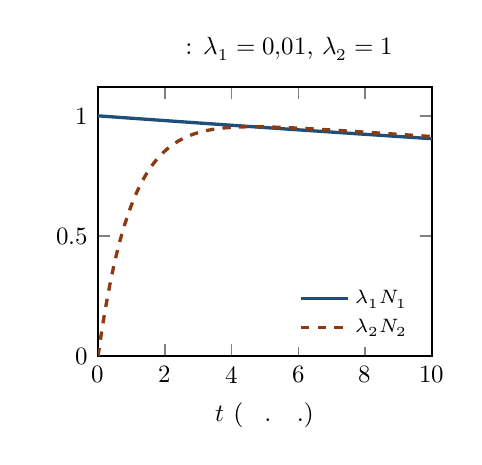
\begin{tikzpicture}
\begin{axis}[width=0.48\linewidth, height=5.0cm, xlabel={$t$ (отн. ед.)}, ylabel={активность}, xmin=0, xmax=10, ymin=0, ymax=1.12,
   samples=200, title={\small вековое: $\lambda_1=0{,}01$, $\lambda_2=1$}, legend style={font=\scriptsize, draw=none}, legend pos=south east]
  \addplot[very thick, accent, domain=0:10] {exp(-0.01*x)};
  \addlegendentry{$\lambda_1N_1$}
  \addplot[very thick, keycol, dashed, domain=0:10] {1/(1-0.01)*(exp(-0.01*x)-exp(-x))};
  \addlegendentry{$\lambda_2N_2$}
\end{axis}
\end{tikzpicture}\hfill
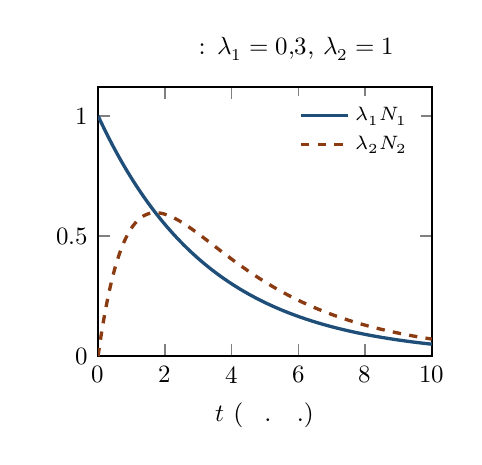
\begin{tikzpicture}
\begin{axis}[width=0.48\linewidth, height=5.0cm, xlabel={$t$ (отн. ед.)}, ylabel={активность}, xmin=0, xmax=10, ymin=0, ymax=1.12,
   samples=200, title={\small подвижное: $\lambda_1=0{,}3$, $\lambda_2=1$}, legend style={font=\scriptsize, draw=none}, legend pos=north east]
  \addplot[very thick, accent, domain=0:10] {exp(-0.3*x)};
  \addlegendentry{$\lambda_1N_1$}
  \addplot[very thick, keycol, dashed, domain=0:10] {1/(1-0.3)*(exp(-0.3*x)-exp(-x))};
  \addlegendentry{$\lambda_2N_2$}
\end{axis}
\end{tikzpicture}
\caption{Активности материнского и дочернего нуклидов (расчёт по~\eqref{eq:18:N2}, $N_2(0)=0$, активности в единицах
$\lambda_1N_{10}$). Слева — установление векового равновесия $\lambda_1N_1=\lambda_2N_2$; справа — подвижное равновесие,
при котором активность дочернего нуклида превышает материнскую.}
\label{fig:18:chain}
\end{figure}

\subsection{Применения}

\paragraph{Радиоактивные семейства.} Тяжёлые природные нуклиды образуют четыре семейства, различающиеся остатком
от деления $A$ на 4 (при $\alpha$-распаде $A$ меняется на 4, при $\beta$-распаде не меняется): $4n$ (родоначальник $\nucl{Th}{232}$,
$T=1{,}4\cdot10^{10}$~лет), $4n+2$ ($\nucl{U}{238}$, $4{,}47\cdot10^9$~лет), $4n+3$ ($\nucl{U}{235}$, $7{,}0\cdot10^8$~лет), $4n+1$ ($\nucl{Np}{237}$,
$2{,}1\cdot10^6$~лет — в природе практически вымерло). Ряд урана заканчивается стабильным $\nucl{Pb}{206}$ после 8 $\alpha$- и
6 $\beta^-$-распадов. В урановой руде все члены ряда находятся в вековом равновесии.

\paragraph{Определение больших периодов полураспада.} Измерив отношение количеств двух членов ряда в равновесной руде и зная
период одного из них, находят период другого по~\eqref{eq:18:secular} (вывод~\ref{der:18:RaU}).

\paragraph{Датирование.} Радиоуглеродный метод: в живых организмах отношение $\nucl{C}{14}/\nucl{C}{12}$ поддерживается постоянным
за счёт обмена с атмосферой (где $\nucl{C}{14}$ образуется космическими лучами); после гибели $\nucl{C}{14}$ распадается с
$T_{1/2}=5730$~лет, и возраст
\begin{equation}\label{eq:18:dating}
  t=\frac{T_{1/2}}{\ln2}\ln\frac{\mathcal A_0}{\mathcal A}.
\end{equation}
Геологический возраст определяют по отношениям $\nucl{Pb}{206}/\nucl{U}{238}$, $\nucl{Ar}{40}/\nucl{K}{40}$ и др.

\section{Математические выводы}

\begin{derivation}[label=der:18:law]{закон радиоактивного распада}
\emph{Допущения:} (1) ядра распадаются независимо друг от друга; (2) вероятность распада ядра за время $\dd t$ равна $\lambda\dd t$ и не
зависит от того, сколько времени ядро уже существует; (3) $N$ велико.

За время $\dd t$ из $N$ ядер в среднем распадается $\dd N_{\text{расп}}=N\lambda\dd t$, поэтому изменение числа ядер
\[
  \dd N=-\lambda N\dd t\quad\Longrightarrow\quad\frac{\dd N}{N}=-\lambda\dd t\quad\Longrightarrow\quad\ln N=-\lambda t+\const .
\]
С начальным условием $N(0)=N_0$: $N(t)=N_0\ee^{-\lambda t}$.

\emph{Вероятностная форма.} Вероятность того, что отдельное ядро не распадётся до момента $t$: $P(t)$. По допущению (2)
$P(t+\dd t)=P(t)(1-\lambda\dd t)$, откуда $\dd P/\dd t=-\lambda P$ и $P(t)=\ee^{-\lambda t}$. Экспоненциальный закон — единственное
распределение времени жизни «без памяти»: $P(t+s\,|\,\text{дожило до }s)=P(t)$.
\end{derivation}

\begin{derivation}[label=der:18:tau]{период полураспада и среднее время жизни}
\emph{Период полураспада.} $N(T_{1/2})=N_0/2$: $\ee^{-\lambda T_{1/2}}=\frac12$ $\Rightarrow$ $T_{1/2}=\ln2/\lambda$.

\emph{Среднее время жизни.} Плотность вероятности распада в момент $t$: $w(t)=-\dd P/\dd t=\lambda\ee^{-\lambda t}$ (нормирована:
$\int_0^\infty w\dd t=1$). Среднее
\[
  \tau=\int_0^\infty t\,\lambda\ee^{-\lambda t}\dd t=\Bigl[-t\ee^{-\lambda t}\Bigr]_0^\infty+\int_0^\infty\ee^{-\lambda t}\dd t=0+\frac1\lambda=\frac1\lambda .
\]
Следовательно, $T_{1/2}=\tau\ln2\approx0{,}693\,\tau$. Эквивалентно: $\tau=\frac{1}{N_0}\int_0^\infty N(t)\dd t$ — «суммарное время жизни всех ядер,
делённое на их число».
\end{derivation}

\begin{derivation}[label=der:18:chain]{решение уравнений цепочки $1\to2\to3$}
\emph{Шаг 1.} $N_1=N_{10}\ee^{-\lambda_1t}$. Подставим во второе уравнение~\eqref{eq:18:chain}:
$\dot N_2+\lambda_2N_2=\lambda_1N_{10}\ee^{-\lambda_1t}$.

\emph{Шаг 2 (интегрирующий множитель $\ee^{\lambda_2t}$).}
\[
  \diff{}{t}\bigl(N_2\ee^{\lambda_2t}\bigr)=\lambda_1N_{10}\ee^{(\lambda_2-\lambda_1)t}
  \ \Rightarrow\
  N_2\ee^{\lambda_2t}=\frac{\lambda_1N_{10}}{\lambda_2-\lambda_1}\ee^{(\lambda_2-\lambda_1)t}+C .
\]
\emph{Шаг 3 (начальное условие $N_2(0)=0$):} $C=-\dfrac{\lambda_1N_{10}}{\lambda_2-\lambda_1}$, и
\[
  N_2(t)=\frac{\lambda_1N_{10}}{\lambda_2-\lambda_1}\Bigl(\ee^{-\lambda_1t}-\ee^{-\lambda_2t}\Bigr).
\]
\emph{Шаг 4 (максимум).} $\dot N_2=0$: $\lambda_1\ee^{-\lambda_1t}=\lambda_2\ee^{-\lambda_2t}$ $\Rightarrow$ $t_m=\dfrac{\ln(\lambda_2/\lambda_1)}{\lambda_2-\lambda_1}$.
В этот момент из~\eqref{eq:18:chain} $\lambda_1N_1=\lambda_2N_2$.

\emph{Шаг 5 (асимптотики).} Отношение активностей
\[
  \frac{\lambda_2N_2}{\lambda_1N_1}=\frac{\lambda_2}{\lambda_2-\lambda_1}\Bigl(1-\ee^{-(\lambda_2-\lambda_1)t}\Bigr)
  \xrightarrow[t\to\infty]{}\frac{\lambda_2}{\lambda_2-\lambda_1}\quad(\lambda_2>\lambda_1).
\]
При $\lambda_1\ll\lambda_2$ предел равен 1 — вековое равновесие~\eqref{eq:18:secular}. Предел $\lambda_1\to\lambda_2$ даёт
$N_2=\lambda_1N_{10}t\ee^{-\lambda_1t}$ (раскрытие неопределённости).

\emph{Вековое уравнение напрямую:} если $N_1$ практически постоянно на временах $\sim\tau_2$, то стационарное решение
второго уравнения~\eqref{eq:18:chain} ($\dot N_2=0$) — $\lambda_1N_1=\lambda_2N_2$; к нему решение приближается как $1-\ee^{-\lambda_2t}$.
\end{derivation}

\begin{derivation}[label=der:18:RaU]{отношение радия к урану в руде}
В равновесном ряду урана $\lambda_{\mathrm U}N_{\mathrm U}=\lambda_{\mathrm{Ra}}N_{\mathrm{Ra}}$, т.\,е.
\[
  \frac{N_{\mathrm{Ra}}}{N_{\mathrm U}}=\frac{T_{\mathrm{Ra}}}{T_{\mathrm U}}=\frac{1600\ \text{лет}}{4{,}47\cdot10^9\ \text{лет}}=3{,}6\cdot10^{-7}.
\]
В 1~т урана содержится $\approx10^6\cdot3{,}6\cdot10^{-7}\cdot\frac{226}{238}\approx0{,}34$~г радия. Наоборот, измерив отношение, можно найти неизвестный
период полураспада урана — время, недоступное прямому наблюдению за убыванием активности.

\emph{Активность 1~г радия:} $\lambda=\frac{0{,}693}{1600\cdot3{,}16\cdot10^7\ \text{с}}=1{,}37\cdot10^{-11}$~с$^{-1}$,
$N=\frac{6{,}02\cdot10^{23}}{226}=2{,}66\cdot10^{21}$, $\mathcal A=\lambda N=3{,}6\cdot10^{10}$~Бк $\approx1$~Ки.
\end{derivation}

\section{Итоговые формулы}

\keyformula{N(t)=N_0\ee^{-\lambda t},\qquad \mathcal A=-\diff Nt=\lambda N}
 {$\lambda$ — постоянная распада, $N_0$ — начальное число ядер, $\mathcal A$ — активность.}
 {большое число независимых ядер; $\lambda$ не зависит от времени.}
 {число ядер и активность в любой момент.}

\keyformula{T_{1/2}=\frac{\ln2}{\lambda},\qquad \tau=\frac1\lambda=\frac{T_{1/2}}{\ln2},\qquad \Gamma=\frac{\hbar}{\tau}}
 {$T_{1/2}$ — период полураспада, $\tau$ — среднее время жизни, $\Gamma$ — ширина уровня.}
 {экспоненциальный распад.}
 {пересчёт характерных времён; связь со спектральной шириной.}

\keyformula{N_2=N_{10}\frac{\lambda_1}{\lambda_2-\lambda_1}\bigl(\ee^{-\lambda_1t}-\ee^{-\lambda_2t}\bigr),\qquad \lambda_1N_1=\lambda_2N_2\ (\lambda_1\ll\lambda_2,\ t\gg\tau_2)}
 {индексы 1 и 2 — материнский и дочерний нуклиды; $N_2(0)=0$.}
 {вековое уравнение — при $T_1\gg T_2$ и времени наблюдения $\gg T_2$.}
 {накопление дочерних продуктов; равновесные отношения в рудах; определение больших $T_{1/2}$.}

\keyformula{t=\frac{T_{1/2}}{\ln2}\ln\frac{\mathcal A_0}{\mathcal A},\qquad \lambda=\sum_i\lambda_i}
 {$\mathcal A_0$ — начальная удельная активность, $\lambda_i$ — парциальные постоянные.}
 {известна начальная активность (радиоуглерод: равновесие с атмосферой).}
 {датирование; ветвление распадов.}

\section{Физическая интерпретация}

\textbf{Статистическая природа.} Экспоненциальный закон — следствие независимости распадов и отсутствия «памяти»;
он не означает, что каждое ядро живёт время $\tau$: время жизни отдельного ядра случайно и распределено
экспоненциально. Отклонения от экспоненты предсказываются квантовой механикой на очень малых и очень больших
временах, но на практике ничтожны.

\textbf{Равновесие как баланс потоков.} Вековое уравнение — аналог стационарного уровня жидкости в сосуде с притоком и
стоком: количество короткоживущего продукта устанавливается таким, чтобы скорость его распада равнялась скорости
образования. Поэтому короткоживущие нуклиды (радий, радон) присутствуют в природе, хотя их периоды много меньше
возраста Земли.

\textbf{Масштабы.} $T_{1/2}$ различаются на десятки порядков; при этом постоянная $\lambda$ — одна из наиболее стабильных величин:
она не меняется при изменении внешних условий в химически и физически доступных пределах, что делает распад
надёжными «часами».

\section{Что необходимо знать на экзамене}

\begin{examcheck}
\checkhead{Определения}
\begin{itemize}
 \item радиоактивность, виды распадов, правила смещения; постоянная распада, $T_{1/2}$, $\tau$, активность (Бк, Ки).
\end{itemize}
\checkhead{Формулы}
\begin{itemize}
 \item $N=N_0\ee^{-\lambda t}$; $T_{1/2}=\ln2/\lambda$; $\tau=1/\lambda$; $\mathcal A=\lambda N$; $\lambda=\sum\lambda_i$;
 \item решение для цепочки $N_2(t)$; вековое уравнение $\lambda_1N_1=\lambda_2N_2$; подвижное равновесие.
\end{itemize}
\checkhead{Выводы}
\begin{itemize}
 \item закон распада из гипотезы постоянной вероятности; $\tau=1/\lambda$ через интеграл;
 \item решение системы для $1\to2\to3$ интегрирующим множителем; три режима; $t_m$.
\end{itemize}
\checkhead{Интерпретации}
\begin{itemize}
 \item почему распад случаен и почему $\lambda$ не зависит от внешних условий;
 \item радиоактивные семейства ($4n$, $4n+1$, $4n+2$, $4n+3$); отношение Ra/U; радиоуглеродное датирование.
\end{itemize}
\end{examcheck}

% ======================================================================
\chapter[Альфа-распад. Закон Гейгера--Нэттола. Формула Гамова]%
        {Альфа-распад. Закон Гейгера--Нэттола и его вывод (формула Гамова)}
\label{t:19}
% ======================================================================

\begin{qbox}
\textbf{Билет 19.} Альфа-распад, закон Гейгера--Нэттола и его вывод (формула Гамова).
\end{qbox}

\section{Содержание билета}

\textbf{Подтемы:}
\begin{enumerate}
 \item альфа-распад: схема, энергия распада, условие энергетической возможности, спектр альфа-частиц;
 \item экспериментальные закономерности: узкий интервал энергий и огромный разброс периодов; закон Гейгера--Нэттола;
 \item парадокс кулоновского барьера и его разрешение туннельным эффектом;
 \item теория Гамова: модель, вычисление проницаемости кулоновского барьера, формула для постоянной распада;
 \item вывод закона Гейгера--Нэттола; численные оценки и границы применимости.
\end{enumerate}

\textbf{Необходимые понятия:} квазиклассическая формула для коэффициента прохождения (\tref{t:07});
закон распада (\tref{t:18}); энергия связи и формула Вайцзеккера (\tref{t:17}); $e^2=1{,}44$~МэВ$\cdot$фм.

\section{Определения и физические принципы}

\begin{definition}[альфа-распад]
Самопроизвольное испускание ядром $\alpha$-частицы (ядра $\nucl{He}{4}$):
\begin{equation}\label{eq:19:scheme}
  \nuc{X}{A}{Z}\ \to\ \nuc{Y}{A-4}{Z-2}+\nuc{He}{4}{2}.
\end{equation}
\emph{Энергия распада} (энерговыделение)
\begin{equation}\label{eq:19:Q}
  Q_\alpha=\bigl[M_{\text{ат}}(A,Z)-M_{\text{ат}}(A-4,Z-2)-M_{\text{ат}}(\nucl{He}{4})\bigr]c^2=E_{\text{св}}(\alpha)+E_{\text{св}}(A-4,Z-2)-E_{\text{св}}(A,Z).
\end{equation}
Распад возможен при $Q_\alpha>0$.
\end{definition}

\begin{principle}{Закон Гейгера--Нэттола}
Для ядер одного радиоактивного ряда (в современной форме — для чётно-чётных ядер с одинаковым $Z$) логарифм периода
полураспада линейно зависит от $Q_\alpha^{-1/2}$:
\begin{equation}\label{eq:19:GN}
  \lg T_{1/2}=a\,\frac{Z}{\sqrt{Q_\alpha}}+b ,
\end{equation}
где $Z$ — заряд дочернего ядра, $a\approx1{,}6$--$1{,}7$ (при $Q$ в МэВ), $b$ слабо зависит от $Z$. Исторически (1911) закон
формулировался как линейная связь $\lg\lambda$ и логарифма пробега $\alpha$-частиц в воздухе.
\end{principle}

\emph{Физический смысл.} Небольшое изменение энергии $\alpha$-частицы меняет время жизни на много порядков: при
$Q_\alpha$ от 4 до 9~МэВ периоды полураспада меняются от $10^{10}$ лет до долей микросекунды. Такая зависимость характерна
для туннельного прохождения барьера: $\lambda\propto\exp(-\text{const}\cdot Z/\sqrt Q)$.

\emph{Область применимости теории Гамова.} Одночастичная модель: $\alpha$-частица считается «готовой» внутри ядра
(вероятность её формирования — множитель порядка $10^{-1}$--$10^{-2}$), ядро сферическое, орбитальный момент вылетающей
частицы $l=0$ (центробежный барьер не учитывается), квазиклассическое приближение ($D\ll1$). Теория предсказывает
$T_{1/2}$ с точностью до 1--2 порядков — достаточно, чтобы объяснить разброс на 24 порядка.

\section{Основная теория}

\subsection{Энергетика альфа-распада}

\paragraph{Условие распада.} $\alpha$-частица очень сильно связана ($E_{\text{св}}=28{,}3$~МэВ, т.\,е. 7,07~МэВ/нуклон). Из~\eqref{eq:19:Q}
$Q_\alpha\approx E_{\text{св}}(\alpha)-4\varepsilon_{\text{эфф}}$, где $\varepsilon_{\text{эфф}}=\Delta E_{\text{св}}/\Delta A$ — энергия связи нуклонов, «отрываемых» от
тяжёлого ядра. Поскольку для $A\gtrsim60$ удельная энергия связи убывает с ростом $A$ (главным образом из-за кулоновского
отталкивания), для достаточно тяжёлых ядер $4\varepsilon_{\text{эфф}}<28{,}3$~МэВ. Формула Вайцзеккера даёт $Q_\alpha>0$ при $A\gtrsim150$;
практически заметный $\alpha$-распад наблюдается у ядер тяжелее свинца (а также у некоторых редкоземельных ядер,
например $\nucl{Sm}{147}$).

\paragraph{Распределение энергии.} Распад двухчастичный, поэтому $\alpha$-частицы \emph{моноэнергетичны} (вывод~\ref{der:19:Talpha}):
\begin{equation}\label{eq:19:Ta}
  T_\alpha=Q_\alpha\frac{M_Y}{M_Y+M_\alpha}\approx Q_\alpha\frac{A-4}{A},
\end{equation}
остальное ($\approx2\,\%$) уносит ядро отдачи. Если распад идёт и на возбуждённые уровни дочернего ядра, в спектре появляются
несколько линий (тонкая структура $\alpha$-спектра), а последующие $\gamma$-кванты уносят разность энергий. Типичные $T_\alpha=4$--$9$~МэВ.

\subsection{Парадокс кулоновского барьера}

Вне ядра на $\alpha$-частицу действует кулоновское отталкивание дочернего ядра, внутри — сильное притяжение
(рис.~\ref{fig:19:pot}). Высота кулоновского барьера при радиусе ядра $R$:
\begin{equation}\label{eq:19:barrier}
  U_B=\frac{2Ze^2}{R}.
\end{equation}
Для урана ($Z=90$, $R\approx9$~фм): $U_B\approx2\cdot90\cdot1{,}44/9\approx29$~МэВ. Опыты Резерфорда по рассеянию $\alpha$-частиц с энергией
$8{,}8$~МэВ на уране не обнаружили отклонений от кулоновского закона — барьер действительно выше 8,8~МэВ. Но сам $\nucl{U}{238}$
испускает $\alpha$-частицы с энергией лишь $4{,}2$~МэВ. Классически частица с энергией $T<U_B$ не может преодолеть барьер ни
изнутри, ни снаружи. Объяснение дали Г.~Гамов и независимо Р.~Гёрни и Э.~Кондон (1928): $\alpha$-частица \emph{туннелирует}
сквозь барьер. Это было первое применение квантовой механики к ядру.

\begin{figure}[htbp]
\centering
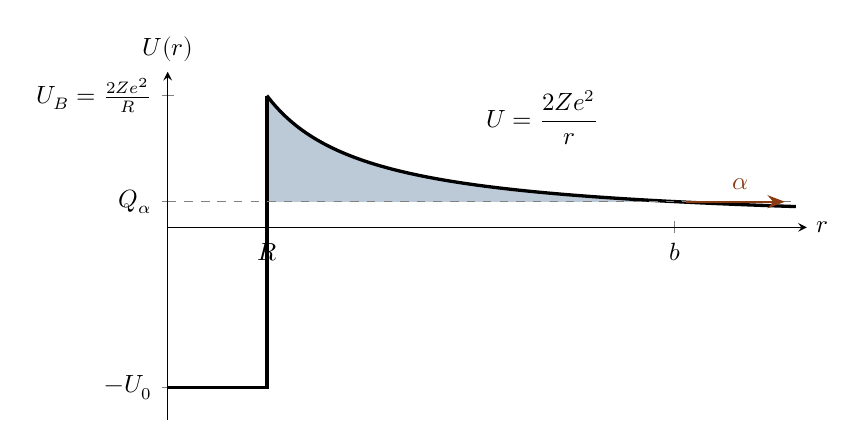
\begin{tikzpicture}
\begin{axis}[width=0.8\linewidth, height=6.0cm, axis lines=middle, xlabel={$r$}, ylabel={$U(r)$},
   xmin=0, xmax=58, ymin=-42, ymax=34, xtick={9,46}, xticklabels={$R$,$b$}, ytick={5.6,28.8,-35},
   yticklabels={$Q_\alpha$,$U_B=\frac{2Ze^2}{R}$,$-U_0$}, samples=200, clip=false,
   xlabel style={at={(ticklabel* cs:1)}, anchor=west}, ylabel style={at={(ticklabel* cs:1)}, anchor=south},
   yticklabel style={font=\small}]
  \addplot[very thick] coordinates {(0,-35) (9,-35) (9,28.8)};
  \addplot[very thick, domain=9:57, name path=C] {259.2/x};
  \addplot[gray, dashed, domain=0:57, name path=E] {5.6};
  \addplot[accent!30] fill between[of=C and E, soft clip={domain=9:46.3}];
  \node[font=\small, accent, anchor=west] at (axis cs:15,8.2) {туннелирование};
  \draw[->, keycol, thick] (axis cs:47,5.6) -- (axis cs:56,5.6);
  \node[font=\small, keycol, anchor=south] at (axis cs:52,6) {$\alpha$};
  \node[font=\small, anchor=west] at (axis cs:28,24) {$U=\dfrac{2Ze^2}{r}$};
  \node[font=\small, align=center] at (axis cs:4.5,-28) {ядерная\\яма};
\end{axis}
\end{tikzpicture}
\caption{Потенциальная энергия $\alpha$-частицы в поле дочернего ядра (модель Гамова): прямоугольная яма глубины $U_0$
при $r<R$ и кулоновский потенциал $2Ze^2/r$ при $r>R$. Под барьером закрашена область $R<r<b$, $b=2Ze^2/Q_\alpha$ —
внешняя точка поворота. Масштаб условный: для $\nucl{U}{238}$ $Q_\alpha\approx4{,}3$~МэВ, $U_B\approx29$~МэВ, $b\approx7R$.}
\label{fig:19:pot}
\end{figure}

\subsection{Теория Гамова}

\paragraph{Модель.} (1) $\alpha$-частица предсуществует в ядре и движется в потенциальной яме радиуса $R$, ударяясь о стенку с
частотой $\nu_0\approx v_{\text{вн}}/2R$; (2) при каждом ударе она проходит барьер с вероятностью $D$; (3) постоянная распада
\begin{equation}\label{eq:19:lambda}
  \lambda=\nu_0D .
\end{equation}
Оценка: скорость внутри ядра $v_{\text{вн}}\sim0{,}1c$ (кинетическая энергия $\sim Q+U_0\sim$ десятки МэВ), $R\sim10$~фм:
$\nu_0\sim3\cdot10^{22}\ \text{фм/с}\cdot0{,}1/(20\ \text{фм})\sim10^{21}$~с$^{-1}$.

\paragraph{Проницаемость барьера.} По квазиклассической формуле (\tref{t:07})
\[
  D\approx\exp\Bigl[-\frac2\hbar\int_R^b\sqrt{2m\Bigl(\frac{2Ze^2}{r}-Q\Bigr)}\,\dd r\Bigr],\qquad b=\frac{2Ze^2}{Q},
\]
где $m$ — приведённая масса $\alpha$-частицы и ядра ($\approx m_\alpha$), $Q\approx T_\alpha$. Вычисление интеграла
(вывод~\ref{der:19:gamow}) даёт \emph{формулу Гамова}
\begin{equation}\label{eq:19:Gamow}
  D\approx\exp\Bigl[-\frac{4\pi Ze^2}{\hbar v}+\frac{8}{\hbar}\sqrt{mZe^2R}\Bigr],\qquad v=\sqrt{\frac{2Q}{m}},
\end{equation}
где $v$ — скорость $\alpha$-частицы на бесконечности. Главный член $2\pi\eta=4\pi Ze^2/\hbar v$ («фактор Гамова») зависит только от
заряда и скорости; второй — поправка на конечный радиус ядра (барьер «срезан» при $r=R$).

\paragraph{Постоянная распада:}
\begin{equation}\label{eq:19:lnlambda}
  \ln\lambda=\ln\nu_0+\frac8\hbar\sqrt{mZe^2R}-\frac{4\pi Ze^2}{\hbar}\sqrt{\frac{m}{2Q}}\,.
\end{equation}

\subsection{Вывод закона Гейгера--Нэттола}

В~\eqref{eq:19:lnlambda} последний член зависит от энергии как $Z/\sqrt Q$, а первые два слабо (логарифмически или через $\sqrt{ZR}$)
зависят от $Z$ и $A$. Для ядер с близкими $Z$ и $A$ (один ряд, или фиксированное $Z$) они практически постоянны. Переходя к
$T_{1/2}=\ln2/\lambda$ и десятичным логарифмам:
\begin{equation}\label{eq:19:GNderived}
  \lg T_{1/2}=\frac{4\pi e^2}{\hbar\ln10}\sqrt{\frac m2}\cdot\frac{Z}{\sqrt Q}+b(Z,R)
  \approx1{,}7\,\frac{Z}{\sqrt{Q\,[\text{МэВ}]}}+b ,
\end{equation}
что и есть закон Гейгера--Нэттола~\eqref{eq:19:GN}, причём коэффициент $a$ выражен через фундаментальные константы
(вывод~\ref{der:19:coef}). Обратно: из сравнения экспериментальных $T_{1/2}$ с~\eqref{eq:19:lnlambda} получают радиусы ядер
$R\approx1{,}4$--$1{,}5\,A^{1/3}$~фм — один из первых методов их определения.

\begin{figure}[htbp]
\centering
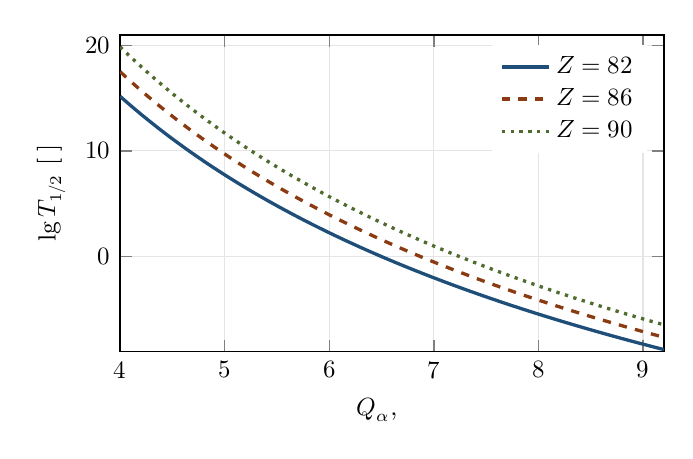
\begin{tikzpicture}
\begin{axis}[width=0.7\linewidth, height=5.6cm, xlabel={$Q_\alpha$, МэВ}, ylabel={$\lg T_{1/2}$ [с]}, xmin=4, xmax=9.2,
   ymin=-9, ymax=21, samples=100, grid=major, grid style={gray!20},
   legend style={font=\small, draw=none}, legend pos=north east,
   declare function={lgT(\Q,\Z)=(0.0917*\Z*43.17/sqrt(\Q)-2.97*sqrt(\Z*1.45*(2.5*\Z)^(1/3)))/2.3026-21.16;}]
  \addplot[very thick, accent, domain=4:9.2] {lgT(x,82)};
  \addlegendentry{$Z=82$}
  \addplot[very thick, keycol, dashed, domain=4:9.2] {lgT(x,86)};
  \addlegendentry{$Z=86$}
  \addplot[very thick, dercol, dotted, domain=4:9.2] {lgT(x,90)};
  \addlegendentry{$Z=90$}
\end{axis}
\end{tikzpicture}
\caption{Оценка периода полураспада по формуле Гамова~\eqref{eq:19:lnlambda} для разных зарядов дочернего ядра
($R=1{,}45A_Y^{1/3}$~фм, $A_Y\approx2{,}5Z$, $\nu_0=10^{21}$~с$^{-1}$; точность оценки — 1--2 порядка). Изменение $Q_\alpha$ вдвое
меняет $T_{1/2}$ более чем на 20 порядков.}
\label{fig:19:GN}
\end{figure}

\paragraph{Факторы, не учтённые простой теорией.} Вероятность образования $\alpha$-кластера в ядре (уменьшает $\lambda$ в 10--100 раз);
центробежный барьер $\hbar^2l(l+1)/2mr^2$ при вылете с $l\neq0$ (замедляет распад); деформация ядра (несферический барьер);
для нечётных ядер распады часто «затруднены» (структурные эффекты). Учёт этих факторов улучшает согласие до множителя
порядка единицы.

\section{Математические выводы}

\begin{derivation}[label=der:19:Talpha]{кинетическая энергия альфа-частицы}
Материнское ядро покоится. Законы сохранения (нерелятивистски, $Q\ll Mc^2$):
\[
  p_\alpha=p_Y\equiv p,\qquad T_\alpha+T_Y=\frac{p^2}{2M_\alpha}+\frac{p^2}{2M_Y}=Q .
\]
Отсюда $\dfrac{T_\alpha}{T_Y}=\dfrac{M_Y}{M_\alpha}$ и
\[
  T_\alpha=Q\frac{M_Y}{M_\alpha+M_Y}\approx Q\frac{A-4}{A},\qquad T_Y=Q\frac{4}{A}.
\]
Для $\nucl{U}{238}$ ($Q=4{,}27$~МэВ): $T_\alpha=4{,}20$~МэВ, $T_Y=0{,}07$~МэВ. Энергия отдачи $\sim70$~кэВ — много больше энергии
химических связей, поэтому дочерние атомы выбиваются из молекул (используется в радиохимии).
\end{derivation}

\begin{derivation}[label=der:19:gamow]{формула Гамова}
\emph{Допущения:} квазиклассика (показатель $\gg1$); $l=0$; барьер — чисто кулоновский при $r>R$; ядро отдачи бесконечно тяжёлое
($m$ — приведённая масса).

\emph{Шаг 1 (интеграл).} Обозначим $b=2Ze^2/Q$ — внешнюю точку поворота. Тогда $\frac{2Ze^2}{r}-Q=Q\bigl(\frac br-1\bigr)$ и
\[
  I\equiv\int_R^b\sqrt{2m\Bigl(\frac{2Ze^2}{r}-Q\Bigr)}\dd r=\sqrt{2mQ}\int_R^b\sqrt{\frac br-1}\,\dd r .
\]
\emph{Шаг 2 (замена $r=b\cos^2u$).} $\dd r=-2b\cos u\sin u\,\dd u$, $\sqrt{b/r-1}=\tg u$. Пределы: $r=b\to u=0$; $r=R\to u_0=\arccos\sqrt{R/b}$:
\[
  \int_R^b\sqrt{\frac br-1}\,\dd r=\int_0^{u_0}\tg u\cdot2b\cos u\sin u\,\dd u=2b\int_0^{u_0}\sin^2u\,\dd u
  =b\bigl[u-\sin u\cos u\bigr]_0^{u_0}.
\]
С $\cos u_0=\sqrt{x}$, $\sin u_0=\sqrt{1-x}$, $x=R/b$:
\[
  I=\sqrt{2mQ}\,b\Bigl[\arccos\sqrt{x}-\sqrt{x(1-x)}\Bigr].
\]
\emph{Шаг 3 (разложение при $x=R/b\ll1$).} Для урана $x\approx0{,}15$. $\arccos\sqrt x\approx\frac\pi2-\sqrt x$, $\sqrt{x(1-x)}\approx\sqrt x$:
\[
  I\approx\sqrt{2mQ}\,b\Bigl(\frac\pi2-2\sqrt{\frac Rb}\Bigr).
\]
\emph{Шаг 4 (подстановка $b$).}
\[
  \frac2\hbar\sqrt{2mQ}\,b\,\frac\pi2=\frac{\pi}{\hbar}\sqrt{2mQ}\frac{2Ze^2}{Q}=\frac{2\pi Ze^2}{\hbar}\sqrt{\frac{2m}{Q}}=\frac{4\pi Ze^2}{\hbar v},
  \quad v=\sqrt{\frac{2Q}{m}};
\]
\[
  \frac2\hbar\sqrt{2mQ}\,b\cdot2\sqrt{\frac Rb}=\frac4\hbar\sqrt{2mQ\,Rb}=\frac4\hbar\sqrt{2mQR\frac{2Ze^2}{Q}}=\frac8\hbar\sqrt{mZe^2R}.
\]
\emph{Итог:} $D=\exp(-2I/\hbar)\approx\exp\Bigl[-\dfrac{4\pi Ze^2}{\hbar v}+\dfrac8\hbar\sqrt{mZe^2R}\Bigr]$.

\emph{Размерности:} $[Ze^2/\hbar v]=\dfrac{\text{эрг}\cdot\text{см}}{\text{эрг}\cdot\text{с}\cdot\text{см}/\text{с}}=1$; $[\sqrt{me^2R}/\hbar]=\dfrac{\sqrt{\text{г}\cdot\text{эрг}\,\text{см}\cdot\text{см}}}{\text{эрг}\,\text{с}}=\dfrac{\text{г}\,\text{см}^2/\text{с}}{\text{г}\,\text{см}^2/\text{с}}=1$.
\end{derivation}

\begin{derivation}[label=der:19:coef]{коэффициент закона Гейгера--Нэттола}
В~\eqref{eq:19:lnlambda} член, зависящий от энергии: $-\dfrac{4\pi Ze^2}{\hbar c}\sqrt{\dfrac{mc^2}{2Q}}=-4\pi\alpha Z\sqrt{\dfrac{mc^2}{2Q}}$. С $mc^2\approx3727$~МэВ:
$\sqrt{mc^2/2}=43{,}2\ \text{МэВ}^{1/2}$, $4\pi\alpha\cdot43{,}2=0{,}0917\cdot43{,}2=3{,}96\ \text{МэВ}^{1/2}$. Тогда
\[
  \ln T_{1/2}=-\ln\lambda+\ln\ln2=3{,}96\frac{Z}{\sqrt{Q[\text{МэВ}]}}+\dots,\qquad
  \lg T_{1/2}=\frac{3{,}96}{2{,}303}\frac{Z}{\sqrt Q}+\dots=1{,}72\frac{Z}{\sqrt Q}+b .
\]
Эмпирический коэффициент $\approx1{,}6$--$1{,}7$ — хорошее согласие (с учётом приведённой массы $m\approx0{,}98m_\alpha$ теоретический
коэффициент $\approx1{,}70$).
\end{derivation}

\begin{derivation}[label=der:19:num]{численная оценка для $\nucl{U}{238}$ и сравнение с $\nucl{Po}{212}$}
\emph{$\nucl{U}{238}\to\nucl{Th}{234}$:} $Z=90$, $Q=4{,}27$~МэВ, $R\approx1{,}45\cdot234^{1/3}\approx8{,}9$~фм.
Первый член: $3{,}96\cdot90/\sqrt{4{,}27}\approx172$. Второй: $\dfrac{8}{\hbar c}\sqrt{mc^2\,Ze^2R}=\dfrac{8\sqrt{3727\cdot90\cdot1{,}44\cdot8{,}9}}{197{,}3}\approx84$.
$\ln D\approx-172+84=-88$, $D\approx4\cdot10^{-39}$. При $\nu_0\sim10^{21}$~с$^{-1}$: $\lambda\sim4\cdot10^{-18}$~с$^{-1}$,
$T_{1/2}\sim2\cdot10^{17}$~с $\sim5\cdot10^9$~лет (опыт: $4{,}47\cdot10^9$~лет). Совпадение по порядку отчасти удачно: изменение $R$ на 10\,\%
меняет второй член на $\approx4$, т.\,е. $T_{1/2}$ — в $\ee^4\approx50$ раз.

\emph{Сравнение:} $\nucl{Po}{212}\to\nucl{Pb}{208}$ ($Z=82$, $Q=8{,}95$~МэВ) имеет $Z/\sqrt Q=27{,}4$ против $43{,}6$ для $\nucl{Th}{232}$ ($Z=88$, $Q=4{,}08$~МэВ).
Разность $16{,}2$ даёт по главному члену $1{,}72\cdot16{,}2\approx28$ порядков; с учётом поправки на радиус — около 26. Опыт:
$T_{1/2}(\nucl{Th}{232})=1{,}4\cdot10^{10}$~лет $=4{,}4\cdot10^{17}$~с, $T_{1/2}(\nucl{Po}{212})=3\cdot10^{-7}$~с — различие в 24 порядка при различии энергий
лишь вдвое.
\end{derivation}

\section{Итоговые формулы}

\keyformula{Q_\alpha=\bigl[M(A,Z)-M(A-4,Z-2)-M(\nucl{He}{4})\bigr]c^2,\qquad T_\alpha\approx Q_\alpha\frac{A-4}{A}}
 {$M$ — массы атомов; $T_\alpha$ — кинетическая энергия $\alpha$-частицы.}
 {распад из основного состояния в основное.}
 {условие распада ($Q>0$), энергия линий $\alpha$-спектра.}

\keyformula{D\approx\exp\Bigl[-\frac{4\pi Ze^2}{\hbar v}+\frac8\hbar\sqrt{mZe^2R}\Bigr],\qquad \lambda=\nu_0D}
 {$Z$ — заряд дочернего ядра, $v=\sqrt{2Q/m}$, $m\approx m_\alpha$, $R$ — радиус ядра, $\nu_0\sim10^{21}$~с$^{-1}$.}
 {квазиклассика, $R\ll b=2Ze^2/Q$, $l=0$, предсуществование $\alpha$-частицы.}
 {постоянная $\alpha$-распада; радиусы ядер по периодам полураспада.}

\keyformula{\lg T_{1/2}=a\frac{Z}{\sqrt{Q_\alpha}}+b,\qquad a=\frac{4\pi\alpha}{\ln10}\sqrt{\frac{mc^2}{2}}\approx1{,}7\ \text{МэВ}^{1/2}}
 {$Q_\alpha$ в МэВ; $b$ слабо зависит от $Z$ и $R$.}
 {ядра с близкими $Z$, $A$; чётно-чётные ядра, $l=0$.}
 {закон Гейгера--Нэттола; экспоненциальная чувствительность к энергии.}

\section{Физическая интерпретация}

\textbf{Почему периоды так различны.} Показатель экспоненты $\sim\pi Ze^2\cdot2/\hbar v\sim100$; изменение энергии на 10\,\% меняет его на 5\,\%,
т.\,е. на несколько единиц — и $T_{1/2}$ на несколько порядков. Поэтому $\alpha$-активные ядра с $Q<4$~МэВ практически стабильны
($T\gg$ возраста Вселенной), а с $Q>9$~МэВ живут микросекунды. Узкий «наблюдаемый» интервал энергий $4$--$9$~МэВ — следствие
этой зависимости.

\textbf{Почему испускаются $\alpha$-частицы, а не протоны или $\nucl{C}{12}$.} Испускание отдельного нуклона обычно энергетически
запрещено ($Q<0$), а $\alpha$-частица очень сильно связана и даёт $Q>0$. Более тяжёлые кластеры ($\nucl{C}{14}$, $\nucl{Ne}{24}$) иногда
энергетически разрешены, но их барьер ($\propto Z_1Z_2$) и масса делают проницаемость ничтожной: кластерный распад наблюдается с
вероятностью $\sim10^{-9}$--$10^{-16}$ относительно $\alpha$-распада.

\textbf{Обращённый процесс.} Тот же фактор Гамова $\exp(-2\pi\eta)$ определяет вероятность сближения заряженных ядер при
термоядерных реакциях в звёздах: синтез при $kT\sim1$~кэВ $\ll$ кулоновского барьера ($\sim1$~МэВ) идёт только благодаря туннелированию.

\section{Что необходимо знать на экзамене}

\begin{examcheck}
\checkhead{Определения}
\begin{itemize}
 \item схема $\alpha$-распада, $Q_\alpha$, условие $Q_\alpha>0$; моноэнергетичность и тонкая структура спектра;
 \item закон Гейгера--Нэттола (формулировка, смысл коэффициентов).
\end{itemize}
\checkhead{Формулы}
\begin{itemize}
 \item $T_\alpha=Q(A-4)/A$; $U_B=2Ze^2/R$; $\lambda=\nu_0D$;
 \item $D\approx\exp[-4\pi Ze^2/\hbar v+(8/\hbar)\sqrt{mZe^2R}]$; $\lg T=aZ/\sqrt Q+b$, $a\approx1{,}7$.
\end{itemize}
\checkhead{Выводы}
\begin{itemize}
 \item парадокс барьера (рассеяние 8,8~МэВ vs испускание 4,2~МэВ) и его разрешение;
 \item вычисление интеграла Гамова (замена $r=b\cos^2u$, разложение при $R\ll b$);
 \item переход к закону Гейгера--Нэттола и оценка коэффициента $a$.
\end{itemize}
\checkhead{Интерпретации}
\begin{itemize}
 \item модель предсуществующей частицы и частоты ударов; неучтённые факторы (образование кластера, $l\neq0$, деформация);
 \item экспоненциальная чувствительность $T_{1/2}$ к $Q$ и $R$; связь с термоядерным синтезом.
\end{itemize}
\end{examcheck}

% ======================================================================
\chapter[Бета-распад ядер. Условия бета-распада]%
        {Бета-распад атомных ядер. Условия бета-распада}
\label{t:20}
% ======================================================================

\begin{qbox}
\textbf{Билет 20.} Бета-распад атомных ядер ($\beta^-$, $\beta^+$, $\mathrm E$-захват), условия бета-распада.
\end{qbox}

\noindent{\small «$\mathrm E$-захват» — электронный захват (захват ядром электрона атомной оболочки; чаще всего с K-оболочки, поэтому
используют и термин «K-захват»).}

\section{Содержание билета}

\textbf{Подтемы:}
\begin{enumerate}
 \item три типа бета-распада: $\beta^-$, $\beta^+$, электронный захват; их нуклонные и кварковые схемы;
 \item энергетические условия бета-распада через массы атомов; распад свободного нейтрона; почему свободный протон стабилен;
 \item непрерывный спектр электронов и гипотеза нейтрино; форма спектра; масса нейтрино; регистрация нейтрино;
 \item электронный захват: условия, сопровождающие явления, случаи «только захват»;
 \item изобарные параболы: бета-стабильность, ядра, распадающиеся обоими способами; времена жизни и правила отбора.
\end{enumerate}

\textbf{Необходимые понятия:} энергия связи и формула Вайцзеккера (\tref{t:17}); слабое взаимодействие (\tref{t:16});
закон распада (\tref{t:18}); фазовый объём (\tref{t:04}); плотность $s$-электронов в ядре (\tref{t:10}).

\section{Определения и физические принципы}

\begin{definition}[бета-распад]
Превращение ядра в изобар с зарядом, отличающимся на единицу, обусловленное слабым взаимодействием:
\begin{align}
  \beta^-:&\quad \nuc{X}{A}{Z}\to\nuc{Y}{A}{Z+1}+e^-+\bar\nu_e &&(n\to p+e^-+\bar\nu_e;\ d\to u+e^-+\bar\nu_e),\label{eq:20:bm}\\
  \beta^+:&\quad \nuc{X}{A}{Z}\to\nuc{Y}{A}{Z-1}+e^++\nu_e &&(p\to n+e^++\nu_e\ \text{в ядре}),\label{eq:20:bp}\\
  \text{E-захват}:&\quad e^-+\nuc{X}{A}{Z}\to\nuc{Y}{A}{Z-1}+\nu_e &&(p+e^-\to n+\nu_e).\label{eq:20:ec}
\end{align}
Массовое число $A$ не меняется; сохраняются электрический заряд, барионное и лептонное числа.
\end{definition}

\begin{definition}[энергия бета-распада]
$Q$ — суммарная кинетическая энергия продуктов, выраженная через массы \emph{атомов} $M(A,Z)$ (см. вывод~\ref{der:20:cond}):
\begin{align}
  Q_{\beta^-}&=\bigl[M(A,Z)-M(A,Z+1)\bigr]c^2, \label{eq:20:Qm}\\
  Q_{\beta^+}&=\bigl[M(A,Z)-M(A,Z-1)-2\mel\bigr]c^2, \label{eq:20:Qp}\\
  Q_{\text{EC}}&=\bigl[M(A,Z)-M(A,Z-1)\bigr]c^2-\varepsilon_i, \label{eq:20:Qec}
\end{align}
где $\varepsilon_i$ — энергия связи захватываемого электрона в оболочке $i$ (K, L,\,\dots). Распад возможен при $Q>0$.
\end{definition}

\emph{Физический смысл.} Бета-распад — способ, которым ядро с «неоптимальным» соотношением $N/Z$ приближается ко дну долины
стабильности (\tref{t:17}): нейтроноизбыточные ядра испытывают $\beta^-$-распад, протоноизбыточные — $\beta^+$-распад или захват.
Электрон и нейтрино не существуют в ядре заранее (электрон в ядре имел бы энергию $\gtrsim40$~МэВ, \tref{t:02}), а рождаются в
момент распада, как фотон при излучении атома.

\emph{Область применимости.} Энергетические условия — точные (с пренебрежением малыми разностями энергий связи атомных
электронов). Форма спектра в простейшей статистической теории — для разрешённых переходов и без учёта кулоновского
взаимодействия электрона с ядром (функции Ферми).

\section{Основная теория}

\subsection{Энергетические условия}

Условия $Q>0$ (вывод~\ref{der:20:cond}) в терминах масс атомов:
\begin{equation}\label{eq:20:conds}
\begin{aligned}
  \beta^-&:\quad M(A,Z)>M(A,Z+1);\\
  \beta^+&:\quad M(A,Z)>M(A,Z-1)+2\mel;\\
  \text{E-захват}&:\quad M(A,Z)>M(A,Z-1)+\varepsilon_i/c^2 .
\end{aligned}
\end{equation}
\textbf{Следствия.}
\begin{enumerate}
 \item Если $\beta^+$-распад возможен, то возможен и захват (условие для захвата слабее на $2\mel c^2=1{,}022$~МэВ); обратное неверно.
 \item При $0<[M(A,Z)-M(A,Z-1)]c^2<1{,}022$~МэВ возможен \emph{только электронный захват}. Пример: $\nucl{Be}{7}\to\nucl{Li}{7}$
       ($Q_{\text{EC}}=0{,}86$~МэВ, $T_{1/2}=53$~сут); $\nucl{Fe}{55}\to\nucl{Mn}{55}$ ($0{,}23$~МэВ).
 \item \textbf{Свободный нейтрон} распадается: $Q=(m_n-m_p-\mel)c^2=0{,}782$~МэВ, $\tau_n\approx880$~с (вывод~\ref{der:20:neutron}).
       \textbf{Свободный протон} стабилен: $m_p<m_n+\mel$. В ядре же протон может превратиться в нейтрон, если энергия связи
       дочернего ядра достаточно велика, т.\,е. энергия берётся из перестройки ядра. Аналогично нейтрон в стабильном ядре не
       распадается, если $M(A,Z+1)>M(A,Z)$.
\end{enumerate}

\subsection{Непрерывный спектр и нейтрино}

\paragraph{Проблема.} $\alpha$-частицы и $\gamma$-кванты моноэнергетичны, а электроны бета-распада имеют \emph{непрерывный} спектр от
нуля до максимальной энергии $T_{\max}\approx Q$ (рис.~\ref{fig:20:spectrum}). Начальное и конечное состояния ядер дискретны, поэтому
двухчастичный распад $X\to Y+e$ давал бы фиксированную энергию электрона. Калориметрические измерения (Эллис и Вустер,
1927) показали, что средняя энергия, выделяемая на один распад, равна среднему $\bar T_e\approx Q/3$, а не $Q$, — часть энергии
«исчезает». Кроме того, нарушался бы закон сохранения момента: например, $\nucl{C}{14}$ и $\nucl{N}{14}$ (чётное $A$) имеют целый спин, а
электрон — полуцелый.

\paragraph{Гипотеза Паули (1930).} Вместе с электроном испускается нейтральная, очень слабо взаимодействующая частица со спином
$\frac12$ и очень малой массой — нейтрино (название дал Ферми). Энергия $Q$ распределяется между тремя телами (электрон,
антинейтрино, ядро отдачи); поскольку ядро тяжёлое, оно почти не уносит энергии, и $T_e+E_\nu\approx Q$. Спектр электронов
непрерывен, а верхняя граница $T_{\max}=Q$ соответствует нулевой энергии нейтрино. Закон сохранения момента
выполняется: $\frac12+\frac12$ — целое.

\paragraph{Теория Ферми (1934).} Распад — превращение $n\to p$ с одновременным рождением пары $e^-\bar\nu$ в одной точке (контактное
слабое взаимодействие, константа $G_F$; на современном языке — обмен виртуальным $W^-$, \tref{t:16}). Вероятность распада
определяется «золотым правилом» $\dd\lambda=\frac{2\pi}{\hbar}|M_{fi}|^2\dd\rho$, где $\dd\rho$ — плотность конечных состояний. Для
разрешённых переходов $|M_{fi}|^2$ от энергии не зависит, и форма спектра определяется фазовым объёмом (вывод~\ref{der:20:spectrum}):
\begin{equation}\label{eq:20:spec}
  \frac{\dd N}{\dd T_e}\propto F(Z,E_e)\,p_eE_e\,(Q-T_e)^2 ,
\end{equation}
где $E_e=T_e+\mel c^2$, $p_e$ — импульс электрона, $F(Z,E_e)$ — функция Ферми, учитывающая притяжение электрона (отталкивание
позитрона) ядром: спектры $\beta^-$ сдвинуты к малым энергиям, $\beta^+$ — к большим.

\begin{figure}[htbp]
\centering
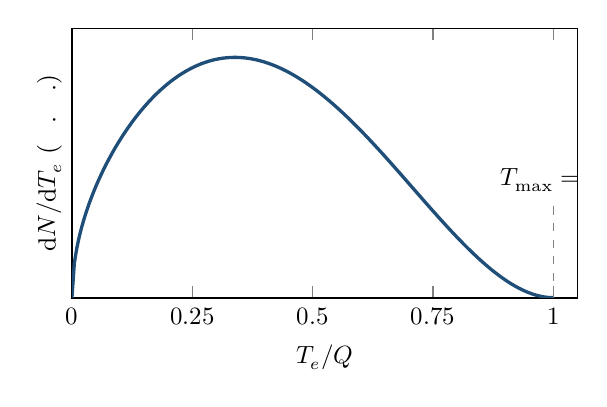
\begin{tikzpicture}
\begin{axis}[width=0.66\linewidth, height=5.0cm, xlabel={$T_e/Q$}, ylabel={$\dd N/\dd T_e$ (отн. ед.)}, xmin=0, xmax=1.05,
   ymin=0, ymax=1.12, samples=200, ytick=\empty, xtick={0,0.25,0.5,0.75,1}]
  \addplot[very thick, accent, domain=0:1] {sqrt(x^2+2*x*0.511)*(x+0.511)*(1-x)^2/0.2523};
  \draw[dashed, gray] (axis cs:1,0) -- (axis cs:1,0.4);
  \node[font=\small, anchor=south] at (axis cs:1,0.4) {$T_{\max}=Q$};
\end{axis}
\end{tikzpicture}
\caption{Форма спектра электронов разрешённого бета-распада по~\eqref{eq:20:spec} без кулоновской поправки
($F=1$), $Q=1$~МэВ. Спектр непрерывен и обрывается при $T_e=Q$; средняя энергия в этом расчёте $\approx0{,}4Q$ (кулоновское притяжение ядра сдвигает спектр $\beta^-$ к меньшим энергиям, и на опыте типично $\bar T_e\approx Q/3$).}
\label{fig:20:spectrum}
\end{figure}

\paragraph{Масса нейтрино.} Если $m_\nu\neq0$, то вблизи верхней границы $(Q-T_e)^2$ заменяется на $(Q-T_e)\sqrt{(Q-T_e)^2-m_\nu^2c^4}$, и
спектр обрывается при $T_e=Q-m_\nu c^2$. Исследование конца спектра трития ($\nucl{H}{3}\to\nucl{He}{3}+e^-+\bar\nu_e$, $Q=18{,}6$~кэВ —
малое $Q$ повышает долю событий у границы) даёт ограничение $m_\nu c^2<0{,}45$~эВ (эксперимент KATRIN). Для удобства анализа
строят \emph{график Кюри}: $\sqrt{N(T)/(pEF)}$ против $T$ — для $m_\nu=0$ и разрешённого перехода это прямая, пересекающая ось при $T=Q$.

\paragraph{Регистрация нейтрино.} Из-за малого сечения ($\sigma\sim10^{-43}$~см$^2$ при энергии $\sim$МэВ) нейтрино прямо
обнаружили лишь в 1956~г. (Ф.~Райнес, К.~Коуэн) у ядерного реактора — мощного источника антинейтрино — по реакции обратного
бета-распада $\bar\nu_e+p\to n+e^+$ (регистрировались совпадения сигнала аннигиляции позитрона и захвата нейтрона).

\subsection{Электронный захват}

Ядро захватывает электрон атомной оболочки, преимущественно с K-оболочки: плотность $s$-электронов в ядре максимальна
и растёт как $Z^3$ (\tref{t:10}). Продукты — ядро $(A,Z-1)$ и моноэнергетическое нейтрино (двухчастичное конечное состояние,
$E_\nu\approx Q_{\text{EC}}$). Сам процесс почти «невидим»; регистрируются сопровождающие явления: на место ушедшего K-электрона
переходят электроны внешних оболочек с испусканием характеристического рентгеновского излучения \emph{дочернего} атома или
оже-электронов. Захват конкурирует с $\beta^+$-распадом: для тяжёлых ядер и малых $Q$ он преобладает (кулоновский барьер
подавляет вылет позитрона, а плотность K-электронов велика). Так как скорость захвата пропорциональна плотности электронов
в ядре, она слегка (порядка $0{,}1\,\%$) зависит от химического окружения — единственный распространённый случай заметной
зависимости $\lambda$ от внешних условий.

\subsection{Изобарные параболы. Бета-стабильность}

Массы изобаров ($A$ фиксировано) по формуле Вайцзеккера — квадратичная функция $Z$ (\tref{t:17}):
\begin{equation}\label{eq:20:parab}
  M(A,Z)c^2=M_0(A)c^2+\frac{\beta(A)}{2}(Z-Z_0)^2-\delta,\qquad \beta(A)=\frac{8a_A}{A}+\frac{2a_C}{A^{1/3}}.
\end{equation}
\begin{itemize}
 \item \textbf{Нечётное $A$} ($\delta=0$): одна парабола. Ядра на левой ветви испытывают $\beta^-$-распад, на правой — $\beta^+$/захват,
       пока не достигнут минимума. Как правило, существует ровно \emph{один} бета-стабильный изобар.
 \item \textbf{Чётное $A$}: две параболы, сдвинутые на $2\delta$ — нижняя для чётно-чётных, верхняя для нечётно-нечётных ядер
       (рис.~\ref{fig:20:parabola}). Распады идут зигзагом между ними. Возможны два и даже три стабильных чётно-чётных изобара
       (их взаимное превращение требует двойного бета-распада, крайне медленного: $T\gtrsim10^{19}$ лет). Нечётно-нечётные ядра
       почти все нестабильны и часто распадаются \emph{обоими} способами: $\nucl{Cu}{64}$ ($\beta^-$ в $\nucl{Zn}{64}$ и $\beta^+$/захват в $\nucl{Ni}{64}$),
       $\nucl{K}{40}$ ($\beta^-$ в $\nucl{Ca}{40}$ — около 89\,\%, захват в $\nucl{Ar}{40}$ — около 11\,\%).
\end{itemize}

\begin{figure}[htbp]
\centering
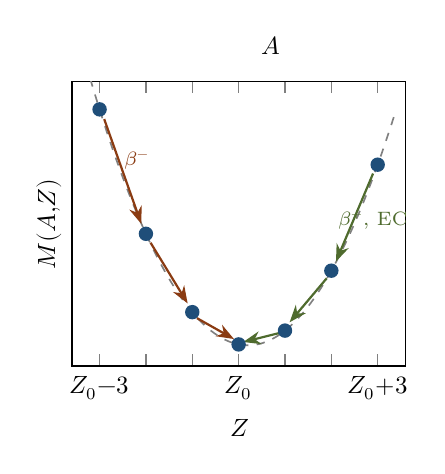
\begin{tikzpicture}
\begin{axis}[width=0.48\linewidth, height=5.2cm, xlabel={$Z$}, ylabel={$M(A,Z)$}, xmin=-3.6, xmax=3.6, ymin=-0.5, ymax=6.3,
   xtick={-3,...,3}, xticklabels={$Z_0{-}3$,,,$Z_0$,,,$Z_0{+}3$}, ytick=\empty, samples=100,
   title={\small нечётное $A$}]
  \addplot[gray, dashed, domain=-3.4:3.4] {0.55*(x-0.2)^2};
  \addplot[only marks, mark=*, mark size=2.3pt, accent] coordinates {(-3,5.632) (-2,2.662) (-1,0.792) (0,0.022) (1,0.352) (2,1.782) (3,4.312)};
  \draw[->, keycol, thick] (axis cs:-2.9,5.4) -- (axis cs:-2.1,2.9);
  \draw[->, keycol, thick] (axis cs:-1.9,2.45) -- (axis cs:-1.1,1.0);
  \draw[->, keycol, thick] (axis cs:-0.9,0.65) -- (axis cs:-0.1,0.15);
  \draw[->, dercol, thick] (axis cs:2.9,4.1) -- (axis cs:2.1,2.0);
  \draw[->, dercol, thick] (axis cs:1.9,1.6) -- (axis cs:1.1,0.55);
  \draw[->, dercol, thick] (axis cs:0.9,0.3) -- (axis cs:0.1,0.08);
  \node[font=\scriptsize, keycol] at (axis cs:-2.2,4.4) {$\beta^-$};
  \node[font=\scriptsize, dercol] at (axis cs:2.9,3.0) {$\beta^+$, EC};
\end{axis}
\end{tikzpicture}\hfill
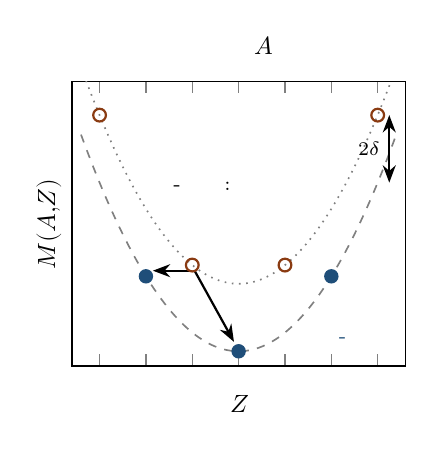
\begin{tikzpicture}
\begin{axis}[width=0.48\linewidth, height=5.2cm, xlabel={$Z$}, ylabel={$M(A,Z)$}, xmin=-3.6, xmax=3.6, ymin=-1.3, ymax=6.3,
   xtick={-3,...,3}, xticklabels={,,,,,,}, ytick=\empty, samples=100,
   title={\small чётное $A$}]
  \addplot[gray, dashed, domain=-3.4:3.4] {0.5*x^2-0.9};
  \addplot[gray, dotted, domain=-3.4:3.4] {0.5*x^2+0.9};
  \addplot[only marks, mark=*, mark size=2.3pt, accent] coordinates {(-2,1.1) (0,-0.9) (2,1.1)};
  \addplot[only marks, mark=o, mark size=2.3pt, keycol, thick] coordinates {(-3,5.4) (-1,1.4) (1,1.4) (3,5.4)};
  \draw[->, thick] (axis cs:-0.95,1.25) -- (axis cs:-0.1,-0.65);
  \draw[->, thick] (axis cs:-1.05,1.25) -- (axis cs:-1.85,1.25);
  \node[font=\scriptsize, align=center] at (axis cs:-1.2,3.2) {нечётно-нечётное:\\распад в обе стороны};
  \node[font=\scriptsize, accent] at (axis cs:2.3,-0.6) {чётно-чётные};
  \draw[<->] (axis cs:3.25,3.6) -- (axis cs:3.25,5.4) node[midway, left, font=\scriptsize] {$2\delta$};
\end{axis}
\end{tikzpicture}
\caption{Изобарные параболы (схема). Слева: нечётное $A$ — единственный стабильный изобар у дна параболы.
Справа: чётное $A$ — две параболы (чётно-чётные ядра — заполненные кружки, нечётно-нечётные — пустые), сдвинутые на $2\delta$;
нечётно-нечётное ядро может распадаться и с увеличением, и с уменьшением $Z$; стабильными могут оказаться несколько
чётно-чётных изобаров.}
\label{fig:20:parabola}
\end{figure}

\subsection{Времена жизни и правила отбора}

Периоды бета-распада — от миллисекунд до $10^{16}$ лет и более. Главные факторы: (1) энерговыделение — при $Q\gg\mel c^2$
$\lambda\propto Q^5$ (закон Сарджента, вывод~\ref{der:20:sargent}); (2) правила отбора. Электрон и нейтрино в разрешённых переходах
вылетают с $l=0$ (их длины волн $\gg R$), поэтому момент ядра может измениться лишь на их суммарный спин:
\emph{фермиевские} переходы (спины $e$ и $\nu$ антипараллельны) — $\Delta J=0$; \emph{гамов-теллеровские} (спины параллельны) —
$\Delta J=0,\pm1$ (кроме $0\to0$); чётность ядра не меняется. Переходы с $l\ge1$ — \emph{запрещённые}, они медленнее на порядки
(множитель $\sim(pR/\hbar)^{2l}$). Для сравнения переходов используют «приведённое время жизни» $fT_{1/2}$, где $f(Z,Q)$ —
интеграл по спектру (для разрешённых $\lg fT\approx3$--$6$).

\section{Математические выводы}

\begin{derivation}[label=der:20:cond]{энергетические условия через массы атомов}
\emph{Обозначения:} $M_{\text я}(Z)$ — масса ядра, $M(Z)=M_{\text я}(Z)+Z\mel-B_e(Z)/c^2$ — масса атома ($B_e$ — энергия связи электронов;
разностью $B_e(Z)-B_e(Z\pm1)$ — десятки эВ--кэВ — пренебрегаем). Масса нейтрино $\approx0$.

\emph{$\beta^-$:} $Q=[M_{\text я}(Z)-M_{\text я}(Z+1)-\mel]c^2$. Подставим $M_{\text я}(Z)=M(Z)-Z\mel$, $M_{\text я}(Z+1)=M(Z+1)-(Z+1)\mel$:
\[
  Q_{\beta^-}=\bigl[M(Z)-Z\mel-M(Z+1)+(Z+1)\mel-\mel\bigr]c^2=\bigl[M(Z)-M(Z+1)\bigr]c^2 .
\]
Масса испущенного электрона «компенсируется» лишним электроном в оболочке дочернего атома.

\emph{$\beta^+$:} $Q=[M_{\text я}(Z)-M_{\text я}(Z-1)-\mel]c^2$:
\[
  Q_{\beta^+}=\bigl[M(Z)-Z\mel-M(Z-1)+(Z-1)\mel-\mel\bigr]c^2=\bigl[M(Z)-M(Z-1)-2\mel\bigr]c^2 .
\]
Один $\mel$ — масса позитрона, второй — лишний электрон оболочки, который «освобождается» (дочерний атом имеет на один
электрон меньше нужного).

\emph{Захват:} начальное состояние — ядро $Z$ и один из его электронов; $Q=[M_{\text я}(Z)+\mel-M_{\text я}(Z-1)]c^2-\varepsilon_i$:
\[
  Q_{\text{EC}}=\bigl[M(Z)-Z\mel+\mel-M(Z-1)+(Z-1)\mel\bigr]c^2-\varepsilon_i=\bigl[M(Z)-M(Z-1)\bigr]c^2-\varepsilon_i .
\]
Таблицы содержат именно атомные массы, поэтому формулы~\eqref{eq:20:Qm}--\eqref{eq:20:Qec} удобны на практике.
\end{derivation}

\begin{derivation}[label=der:20:neutron]{распад нейтрона и стабильность протона}
$Q_n=(m_n-m_p-\mel)c^2=939{,}565-938{,}272-0{,}511=0{,}782$~МэВ $>0$ — нейтрон распадается.
Максимальная кинетическая энергия электрона $\approx0{,}782$~МэВ (отдача протона: при максимальном импульсе электрона
$pc=\sqrt{T(T+2\mel c^2)}\approx1{,}19$~МэВ протон получает $p^2/2m_p\approx0{,}75$~кэВ — пренебрежимо).

Для свободного протона: $Q=(m_p-m_n-\mel)c^2=-1{,}80$~МэВ $<0$ — распад $p\to ne^+\nu$ невозможен. Захват $p+e^-\to n+\nu$ (атом водорода):
$Q=(m_{\mathrm H}-m_n)c^2\approx-0{,}78$~МэВ — тоже невозможен. В ядрах эти процессы идут за счёт разности энергий связи:
$Q_{\beta^+}=Q_{\text{нукл}}+[E_{\text{св}}(Z-1)-E_{\text{св}}(Z)]$.
\end{derivation}

\begin{derivation}[label=der:20:spectrum]{форма бета-спектра из фазового объёма}
\emph{Допущения:} разрешённый переход ($|M_{fi}|$ не зависит от энергий); нейтрино безмассово; отдачей ядра пренебрегаем
(оно уносит импульс, но не энергию); кулоновское поле ядра не учитывается ($F=1$).

\emph{Шаг 1.} Число состояний электрона и нейтрино в объёме $V$ (\tref{t:04}):
$\dd n=\dfrac{V\,4\pi p_e^2\dd p_e}{(2\pi\hbar)^3}\cdot\dfrac{V\,4\pi p_\nu^2\dd p_\nu}{(2\pi\hbar)^3}$ (импульс ядра фиксирован законом сохранения).

\emph{Шаг 2.} Энергия сохраняется: $T_e+E_\nu=Q$, $E_\nu=p_\nu c$. При фиксированном $p_e$ плотность состояний на единицу полной
энергии получается заменой $\dd p_\nu=\dd E_\nu/c$: $\dd\rho\propto p_e^2\dd p_e\cdot p_\nu^2/c$, где $p_\nu=(Q-T_e)/c$.

\emph{Шаг 3.} Переход к переменной $T_e$: из $E_e^2=p_e^2c^2+\mel^2c^4$ $\Rightarrow$ $p_e\dd p_e=E_e\dd E_e/c^2=E_e\dd T_e/c^2$. Итого
\[
  \frac{\dd N}{\dd T_e}\propto p_e^2\frac{\dd p_e}{\dd T_e}(Q-T_e)^2=p_eE_e(Q-T_e)^2/c^2 .
\]
\emph{Анализ:} при $T_e\to0$ $\dd N/\dd T_e\propto p_e\to0$ (мало состояний электрона); при $T_e\to Q$ $\propto(Q-T_e)^2\to0$ (мало состояний
нейтрино). Максимум — в средней части спектра; при $Q=1$~МэВ и $F=1$ численное интегрирование даёт $\bar T_e\approx0{,}4Q$, а с учётом функции Ферми для $\beta^-$-распада — около $Q/3$.
\end{derivation}

\begin{derivation}[label=der:20:sargent]{закон Сарджента для бета-распада}
Полная вероятность $\lambda\propto\int_0^Q p_eE_e(Q-T_e)^2\dd T_e$. В ультрарелятивистском пределе $Q\gg\mel c^2$: $p_ec\approx E_e\approx T_e$:
\[
  \lambda\propto\int_0^QT^2(Q-T)^2\dd T=Q^5\int_0^1x^2(1-x)^2\dd x=Q^5\Bigl(\frac13-\frac24+\frac15\Bigr)=\frac{Q^5}{30}.
\]
Таким образом $\lambda\propto G_F^2Q^5$ — результат, согласующийся с размерным анализом для распада мюона (\tref{t:16}).
Удвоение энергии распада уменьшает время жизни в $\approx30$ раз. При $Q\lesssim\mel c^2$ электрон нерелятивистский, зависимость от $Q$ другая, и закон $Q^5$ даёт лишь грубую оценку.
\end{derivation}

\begin{derivation}[label=der:20:parab]{бета-стабильность и изобарная парабола}
Из~\eqref{eq:20:parab} при нечётном $A$ разность масс соседних изобаров
\[
  [M(Z)-M(Z+1)]c^2=\frac\beta2\bigl[(Z-Z_0)^2-(Z+1-Z_0)^2\bigr]=\beta\Bigl(Z_0-Z-\frac12\Bigr).
\]
$\beta^-$-распад $Z\to Z+1$ возможен при $Z<Z_0-\frac12$; аналогично $\beta^+$/захват $Z\to Z-1$ — при $Z>Z_0+\frac12$ (для захвата;
для $\beta^+$ — при большем удалении, с учётом $2\mel c^2$). Стабилен изобар с $|Z-Z_0|<\frac12$ — как правило, единственный.

При чётном $A$ для нечётно-нечётного ядра $Z$ оба соседа — чётно-чётные и лежат на параболе ниже на $2\delta$:
$[M(Z)-M(Z\pm1)]c^2=2\delta+\beta(\dots)$. Если $2\delta$ превышает разность ординат параболы, распад энергетически возможен в обе
стороны — так распадаются $\nucl{Cu}{64}$ и $\nucl{K}{40}$.
\end{derivation}

\section{Итоговые формулы}

\keyformula{Q_{\beta^-}=[M(Z)-M(Z+1)]c^2,\quad Q_{\beta^+}=[M(Z)-M(Z-1)-2\mel]c^2,\quad Q_{\text{EC}}=[M(Z)-M(Z-1)]c^2-\varepsilon_i}
 {$M$ — массы нейтральных атомов, $\varepsilon_i$ — энергия связи захватываемого электрона.}
 {пренебрегаем разностью энергий связи атомных электронов и массой нейтрино.}
 {энергетические условия и энерговыделение всех типов бета-распада.}

\keyformula{\frac{\dd N}{\dd T_e}\propto F(Z,E_e)\,p_eE_e(Q-T_e)^2,\qquad T_{\max}=Q-m_\nu c^2}
 {$T_e$, $E_e$, $p_e$ — кинетическая, полная энергия и импульс электрона; $F$ — функция Ферми.}
 {разрешённые переходы; отдача ядра пренебрежима.}
 {форма непрерывного спектра; масса нейтрино по концу спектра.}

\keyformula{n\to p+e^-+\bar\nu_e:\ Q=0{,}782\ \text{МэВ},\ \ \tau\approx880\ \text{с};\qquad \lambda\propto Q^5\ (Q\gg\mel c^2)}
 {$Q$ — энергия распада.}
 {закон Сарджента — для разрешённых переходов при больших $Q$.}
 {стабильность нуклонов; оценка относительных времён жизни.}

\keyformula{M(A,Z)c^2=M_0c^2+\frac\beta2(Z-Z_0)^2-\delta,\qquad Z_0\approx\frac{A}{1{,}98+0{,}015A^{2/3}}}
 {$\beta=8a_A/A+2a_C/A^{1/3}$, $\delta$ — энергия спаривания.}
 {капельная модель.}
 {какие изобары стабильны, направление бета-распада, двусторонние распады нечётно-нечётных ядер.}

\section{Физическая интерпретация}

\textbf{Роль бета-распада.} Сильное взаимодействие формирует ядро, но не может менять $N/Z$; это делает слабое взаимодействие.
Поэтому бета-распады медленные (от миллисекунд до миллиардов лет), а распределение стабильных ядер на плоскости $(N,Z)$ —
узкая долина, по склонам которой ядра «скатываются» бета-распадами.

\textbf{Нейтрино.} Непрерывный спектр — главный экспериментальный аргумент в пользу нейтрино. Оно уносит в среднем около
двух третей энергии распада, что важно для энергетики реакторов и звёзд (нейтринные потери).

\textbf{Сравнение трёх процессов.} $\beta^-$ — избыток нейтронов; $\beta^+$ и захват — избыток протонов, причём при $\Delta Mc^2<1{,}022$~МэВ
возможен только захват. Захват даёт моноэнергетические нейтрино и рентгеновское излучение дочернего атома; $\beta^+$ —
аннигиляционные $\gamma$-кванты по $0{,}511$~МэВ (основа позитронно-эмиссионной томографии).

\section{Что необходимо знать на экзамене}

\begin{examcheck}
\checkhead{Определения}
\begin{itemize}
 \item схемы $\beta^-$, $\beta^+$, E-захвата на уровне ядер, нуклонов и кварков; законы сохранения ($Q$, $B$, $L_e$, момент);
 \item непрерывный спектр, гипотеза нейтрино (энергия и момент), обнаружение нейтрино (Райнес--Коуэн).
\end{itemize}
\checkhead{Формулы}
\begin{itemize}
 \item условия распада через атомные массы: $M(Z)>M(Z+1)$; $M(Z)>M(Z-1)+2\mel$; $M(Z)>M(Z-1)+\varepsilon/c^2$;
 \item $Q_n=0{,}782$~МэВ; форма спектра $p_eE_e(Q-T_e)^2$; $\lambda\propto Q^5$; изобарная парабола.
\end{itemize}
\checkhead{Выводы}
\begin{itemize}
 \item переход от ядерных масс к атомным в условиях $\beta^\pm$ и захвата (откуда $2\mel$);
 \item форма спектра из фазового объёма; закон Сарджента (интеграл $Q^5/30$);
 \item бета-стабильность для нечётных и чётных $A$.
\end{itemize}
\checkhead{Интерпретации}
\begin{itemize}
 \item почему свободный протон стабилен, а в ядре возможен $\beta^+$-распад; случаи «только захват» ($\nucl{Be}{7}$);
 \item двусторонние распады ($\nucl{Cu}{64}$, $\nucl{K}{40}$); правила отбора Ферми и Гамова--Теллера; масса нейтрино по спектру трития.
\end{itemize}
\end{examcheck}


\end{document}
